\documentclass[../main.tex]{subfiles}

\begin{document}

\chapter{Results}

After the simulation ended, the displacement and stress results of the surface and volume meshes were exported as a .csv file. The surface mesh was utilized to gather statistics on the displacement of the part, to understand its overall deformation. The volume mesh was used to analyze the stress distribution within the component. R consisted of the node displacement and stress values. This information was then analyzed using R, and various plots were created using the ggplot library. 

The values that are most important for this study are the average values and the maximum values, as both of these could be taken to be different criteria to compare performances. Obviously, a part with lower average displacement or lower stress will be more desirable, but it is also important to consider maximum displacement and maximum stress as well, as a part with lower average displacement but with a few nodes with very high displacement could still be considered a failed component, as it is the portions with highest deformation that will need to be processed with additional machining, or cause high discomfort in patients. Additionally, regions of maximum stress should be considered because the stress at this regions might be greater than the ultimate stress of the material, causing the component to break and fail.


\section{Results of simple geometry simulations}

This section shows the results for the simple geometry simulations, composed of a cube, three triangles with different angles, and three cubes with fillets, as explained in Chapter \ref{ch:cad}.


The results of the analysis indicate that there is no apparent relationship between the hyperbolic angle or boundary conditions and the observed node displacements. The average node displacements for each topology and each project appear to be relatively stable, with no stark differences observed between the various topologies. The differences in node displacements between the topologies fall well within the uncertainty bounds of the convergence results, suggesting that the choice of topology does not have a significant impact on the overall structural behavior. These findings imply that the design parameters under investigation, such as the hyperbolic angle and boundary conditions, do not play a dominant role in driving the global structural response, at least within the range of values considered in this study. 

In addition to the node displacements, the analysis also examined the average node stress and maximum node stress for each topology and project. These stress metrics were found to follow a similar trend as the average node displacements, exhibiting relatively stable values across the different topologies with no clear relationship between topology and stress levels. The differences in both average and maximum node stresses between the various topologies fall within the uncertainty bounds of the convergence results, suggesting that the choice of topology does not have a significant impact on the overall stress state of the structure. This further reinforces the conclusion that the design parameters investigated, such as the hyperbolic angle and boundary conditions, do not play a dominant role in driving the global structural response in terms of both displacements and stresses. The consistent stress and displacement behavior across topologies indicates a level of robustness in the structural performance that may be advantageous for design applications where flexibility and insensitivity to specific design choices are desirable.

While the overall trends indicate a general stability in the average node displacements and stresses across the different topologies, the analysis also revealed some notable exceptions. Specifically, certain topologies were found to result in significantly higher maximum node displacements that could not be attributed solely to the uncertainty of the convergence results. This behavior was most pronounced in the 15\degree, 30\degree, and 45\degree triangle components, where some topologies exhibited much greater maximum displacements compared to others. The fillet components showed the most obvious differences, with variations in maximum nodal displacement of up to 0.2 mm between certain topologies. In contrast, the cube components did not display this trend as strongly, suggesting that the sensitivity to topology may be more pronounced in certain geometric configurations. These findings indicate that while the average structural response may be relatively insensitive to topology, the choice of topology can have a significant impact on the localized maximum displacements in specific regions of the structure. This information may be valuable for design optimization efforts that prioritize limiting peak displacements or stresses in critical areas.

One final note before finishing this section. When the parameters of geometry were varied according to the tables in Chapter \ref{ch:params}, some of the resulting topologies were very similar to each other, and others were deemed to be undesirable, due to very small thin supports. These repeated and faulty topologies were discarded and were not used for the manufacturing simulation. This resulted in different groups being used for each geometry study, as can be seen in the members of each graph.

Graphs summarizing these results are shown below. Figure \ref{fig:cuberesults} show the results for the cubic component. Figures \ref{fig:tri15_results}, \ref{fig:tri30_results}, and \ref{fig:tri45_results} show the results for all the triangular components, while Figures \ref{fig:20r_results}, \ref{fig:30r_results}, and \ref{fig:40r_results} show the results of the components with fillets. Each of the bars in the figures below represents a particular combination of parameters belonging to a topology resulting from the COMSOL simulation. Figure \ref{fig:key} explains what each x-axis label means. The parameters shown in the key are the same parameters explained in Table \ref{tab:params}.

\begin{figure}[h!]
  \centering
  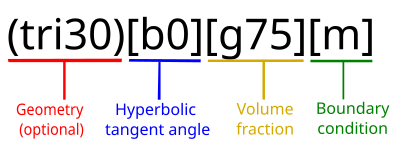
\includegraphics[width=0.5\textwidth]{key.png}
  \caption{Topology key explanation.}
  \label{fig:key}
  \end{figure}

\begin{figure}[h!]
  \centering 
  \begin{subfigure}[b]{0.45\textwidth}
    \centering 
    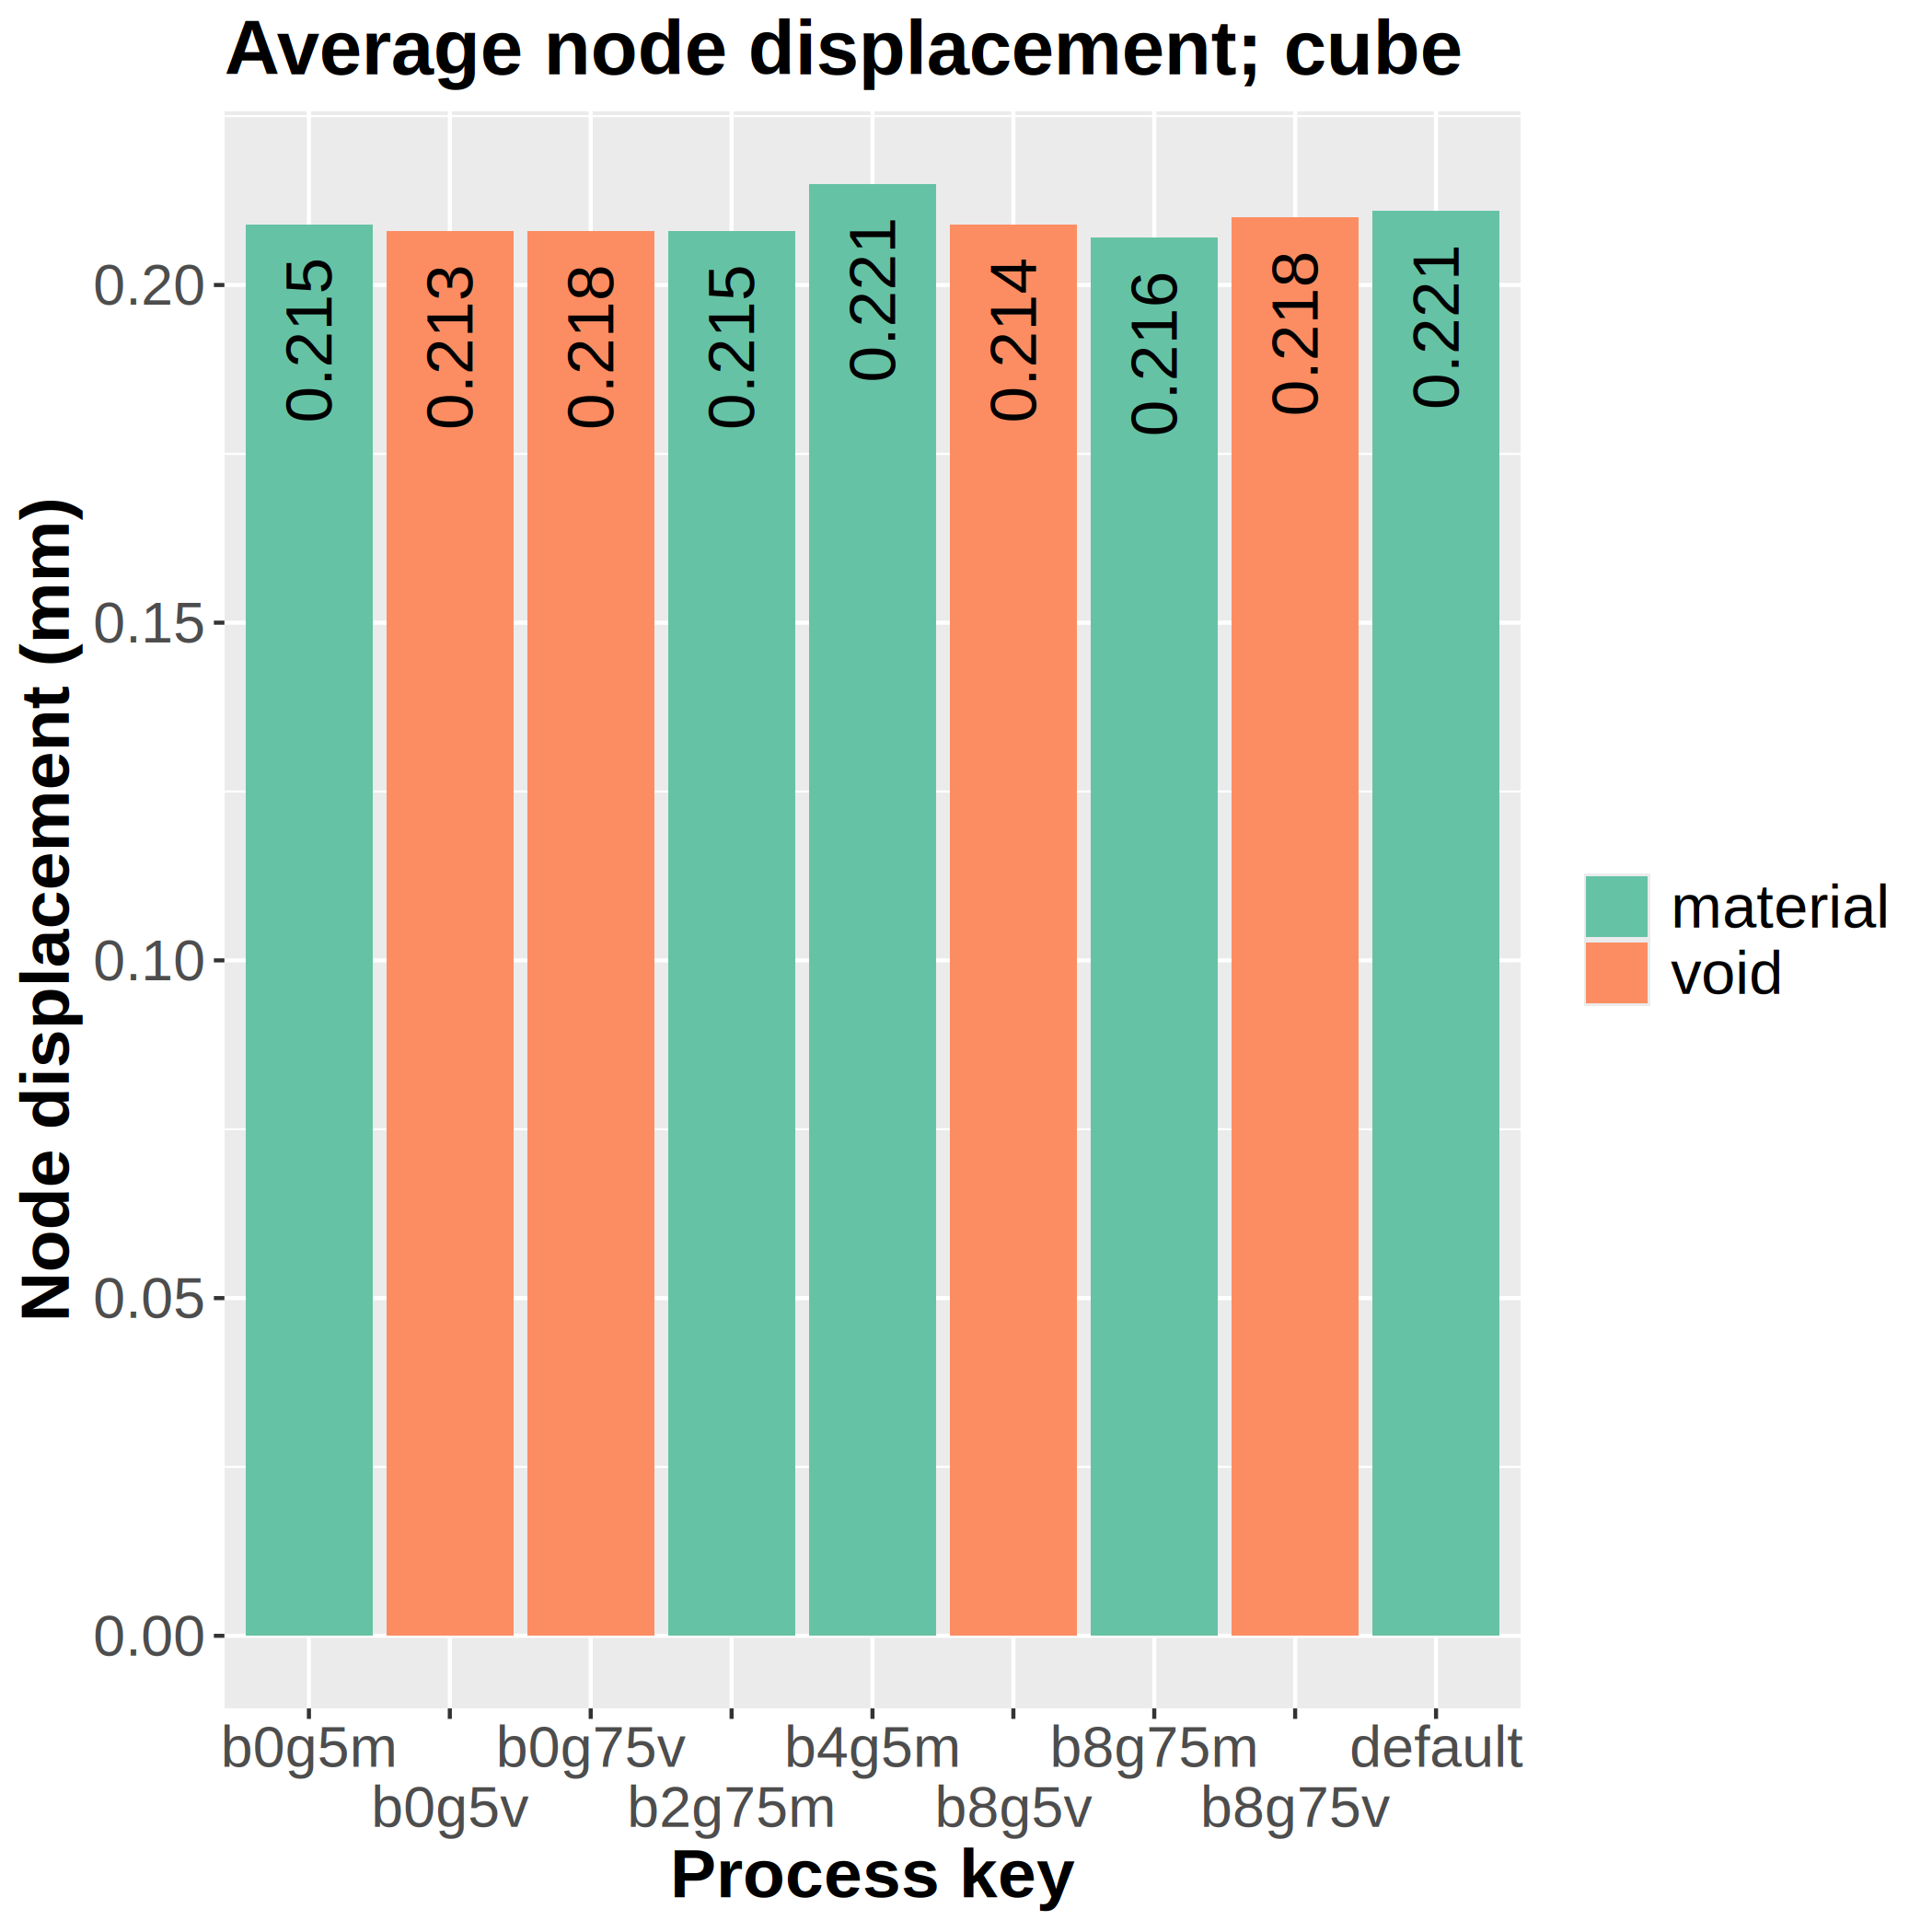
\includegraphics[width=\textwidth]{cube _disp3.png}
    \label{}
  \end{subfigure}
  \begin{subfigure}[b]{0.45\textwidth}
    \centering 
    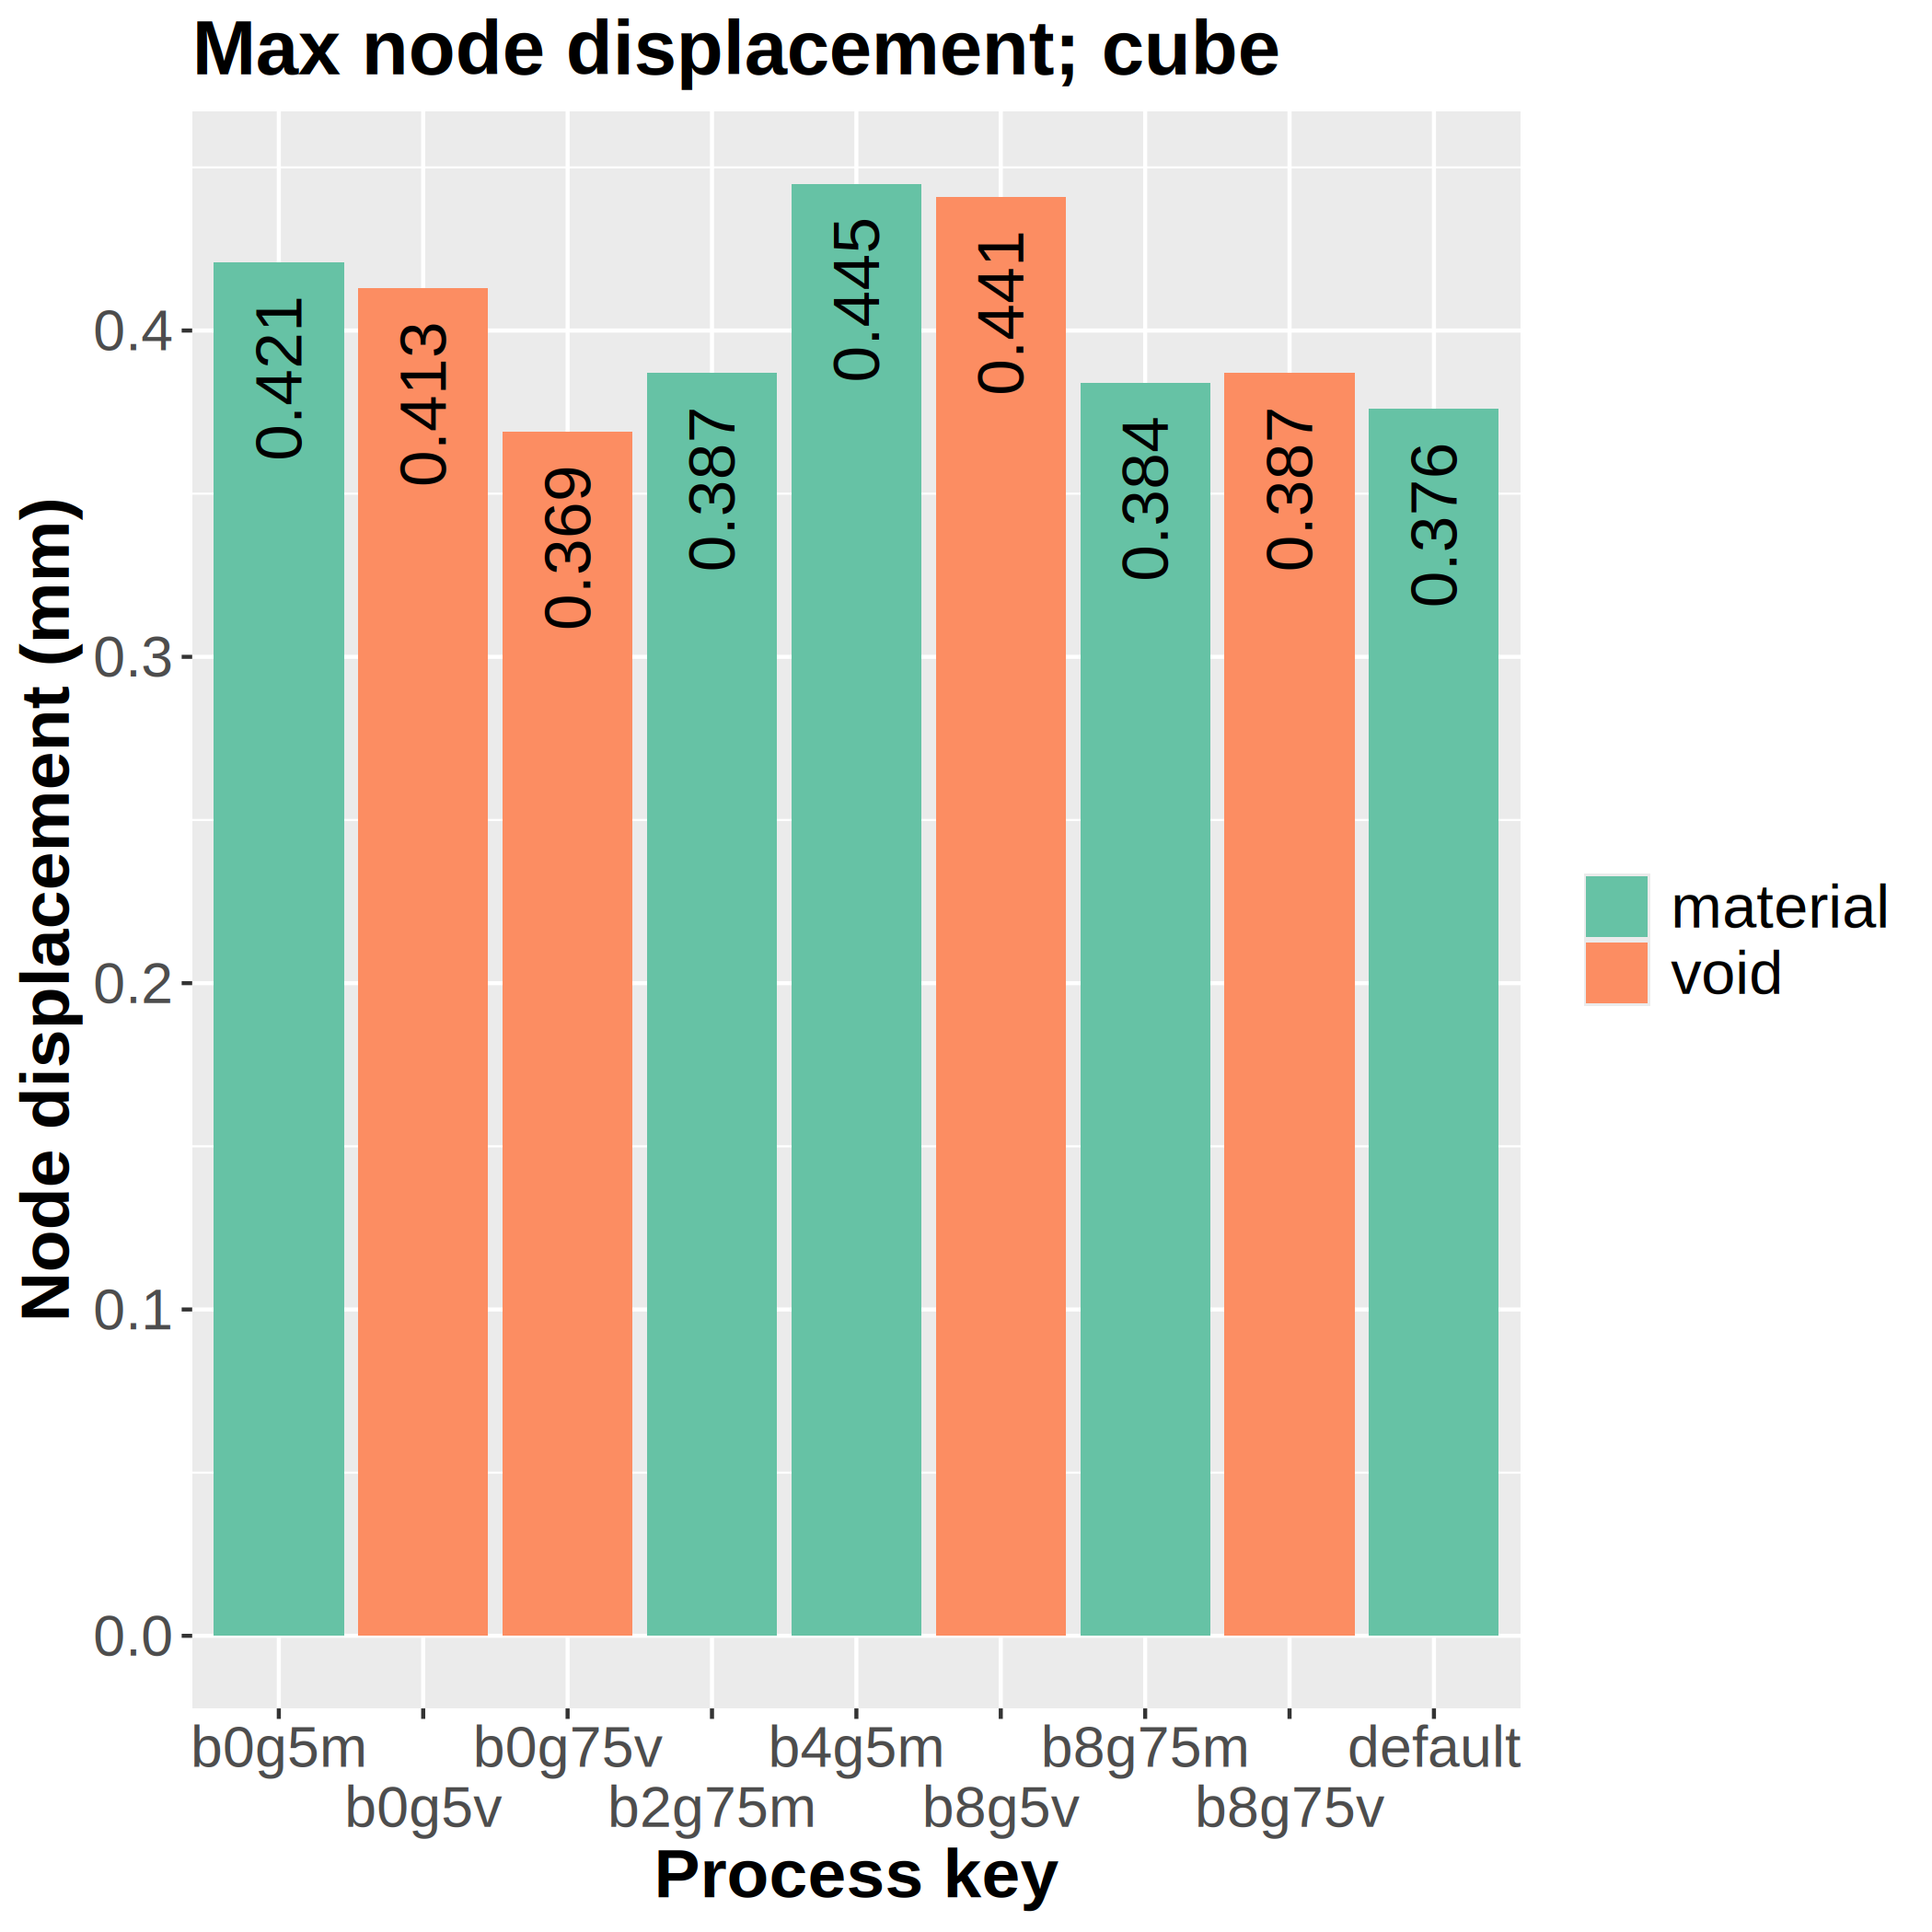
\includegraphics[width=\textwidth]{cube _dispmax3.png}
    \label{}
  \end{subfigure}
  \begin{subfigure}[b]{0.45\textwidth}
    \centering 
    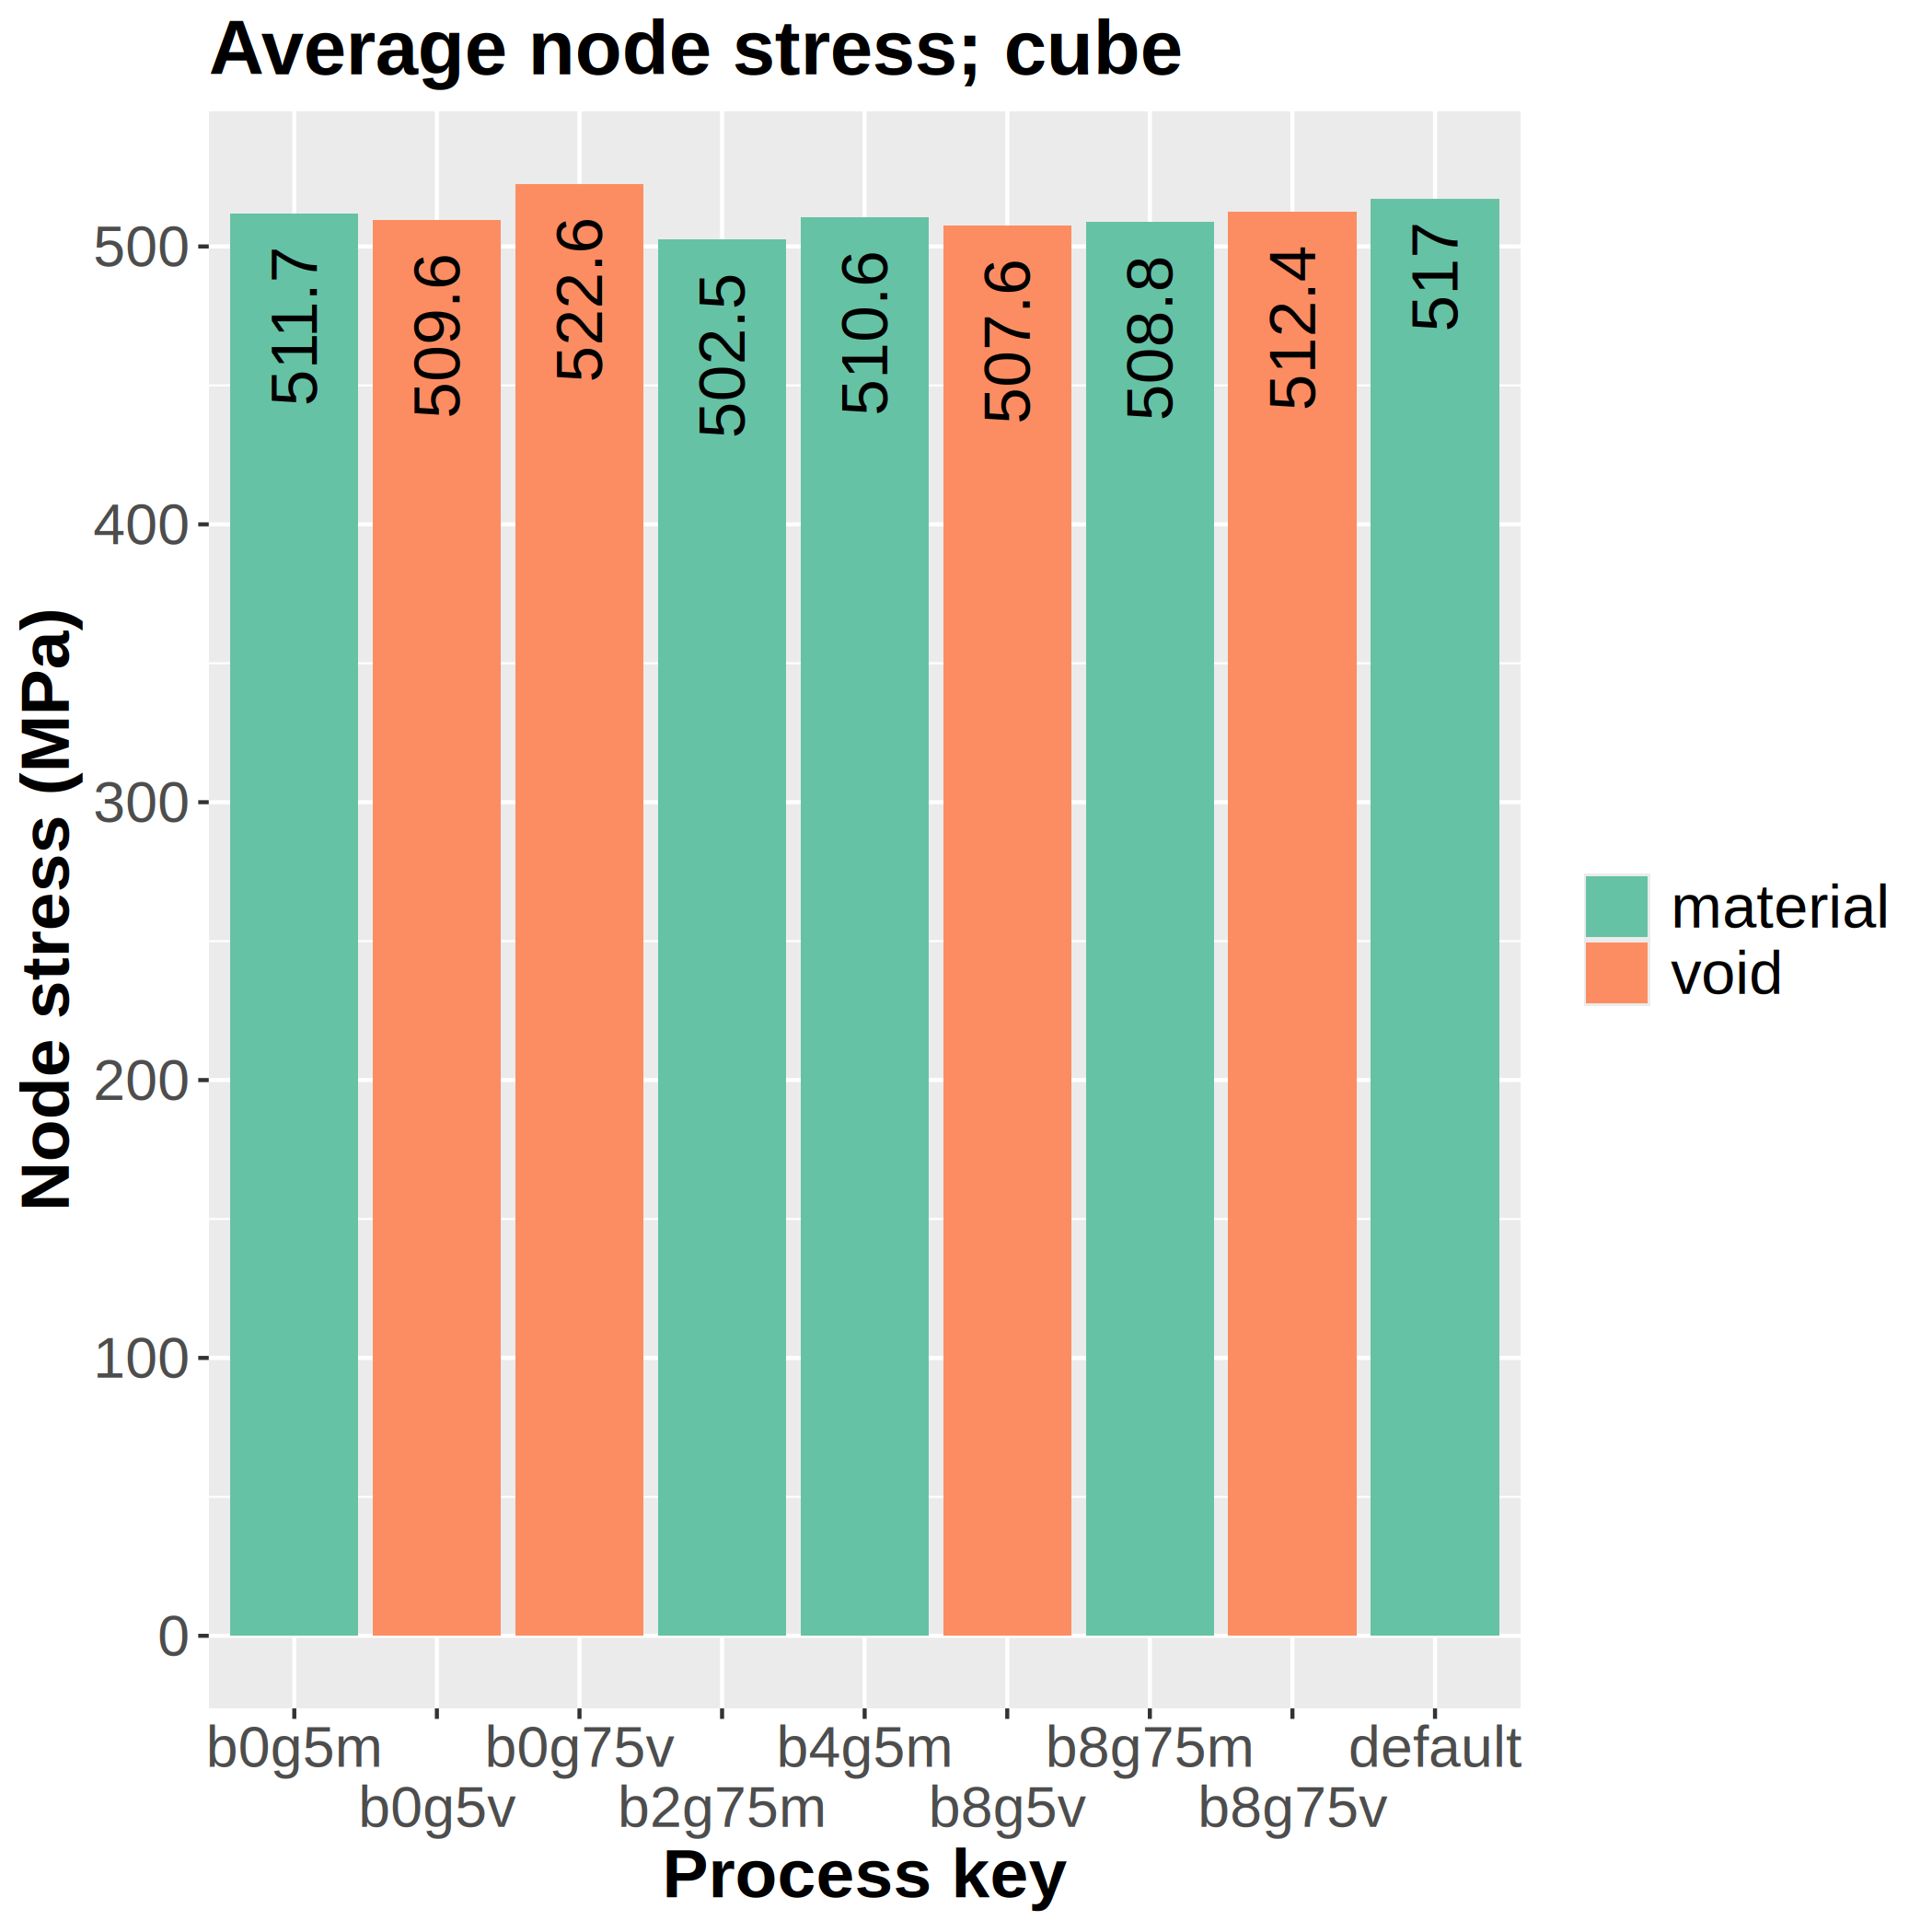
\includegraphics[width=\textwidth]{cube _stress3.png}
    \label{}
  \end{subfigure}
  \begin{subfigure}[b]{0.45\textwidth}
    \centering 
    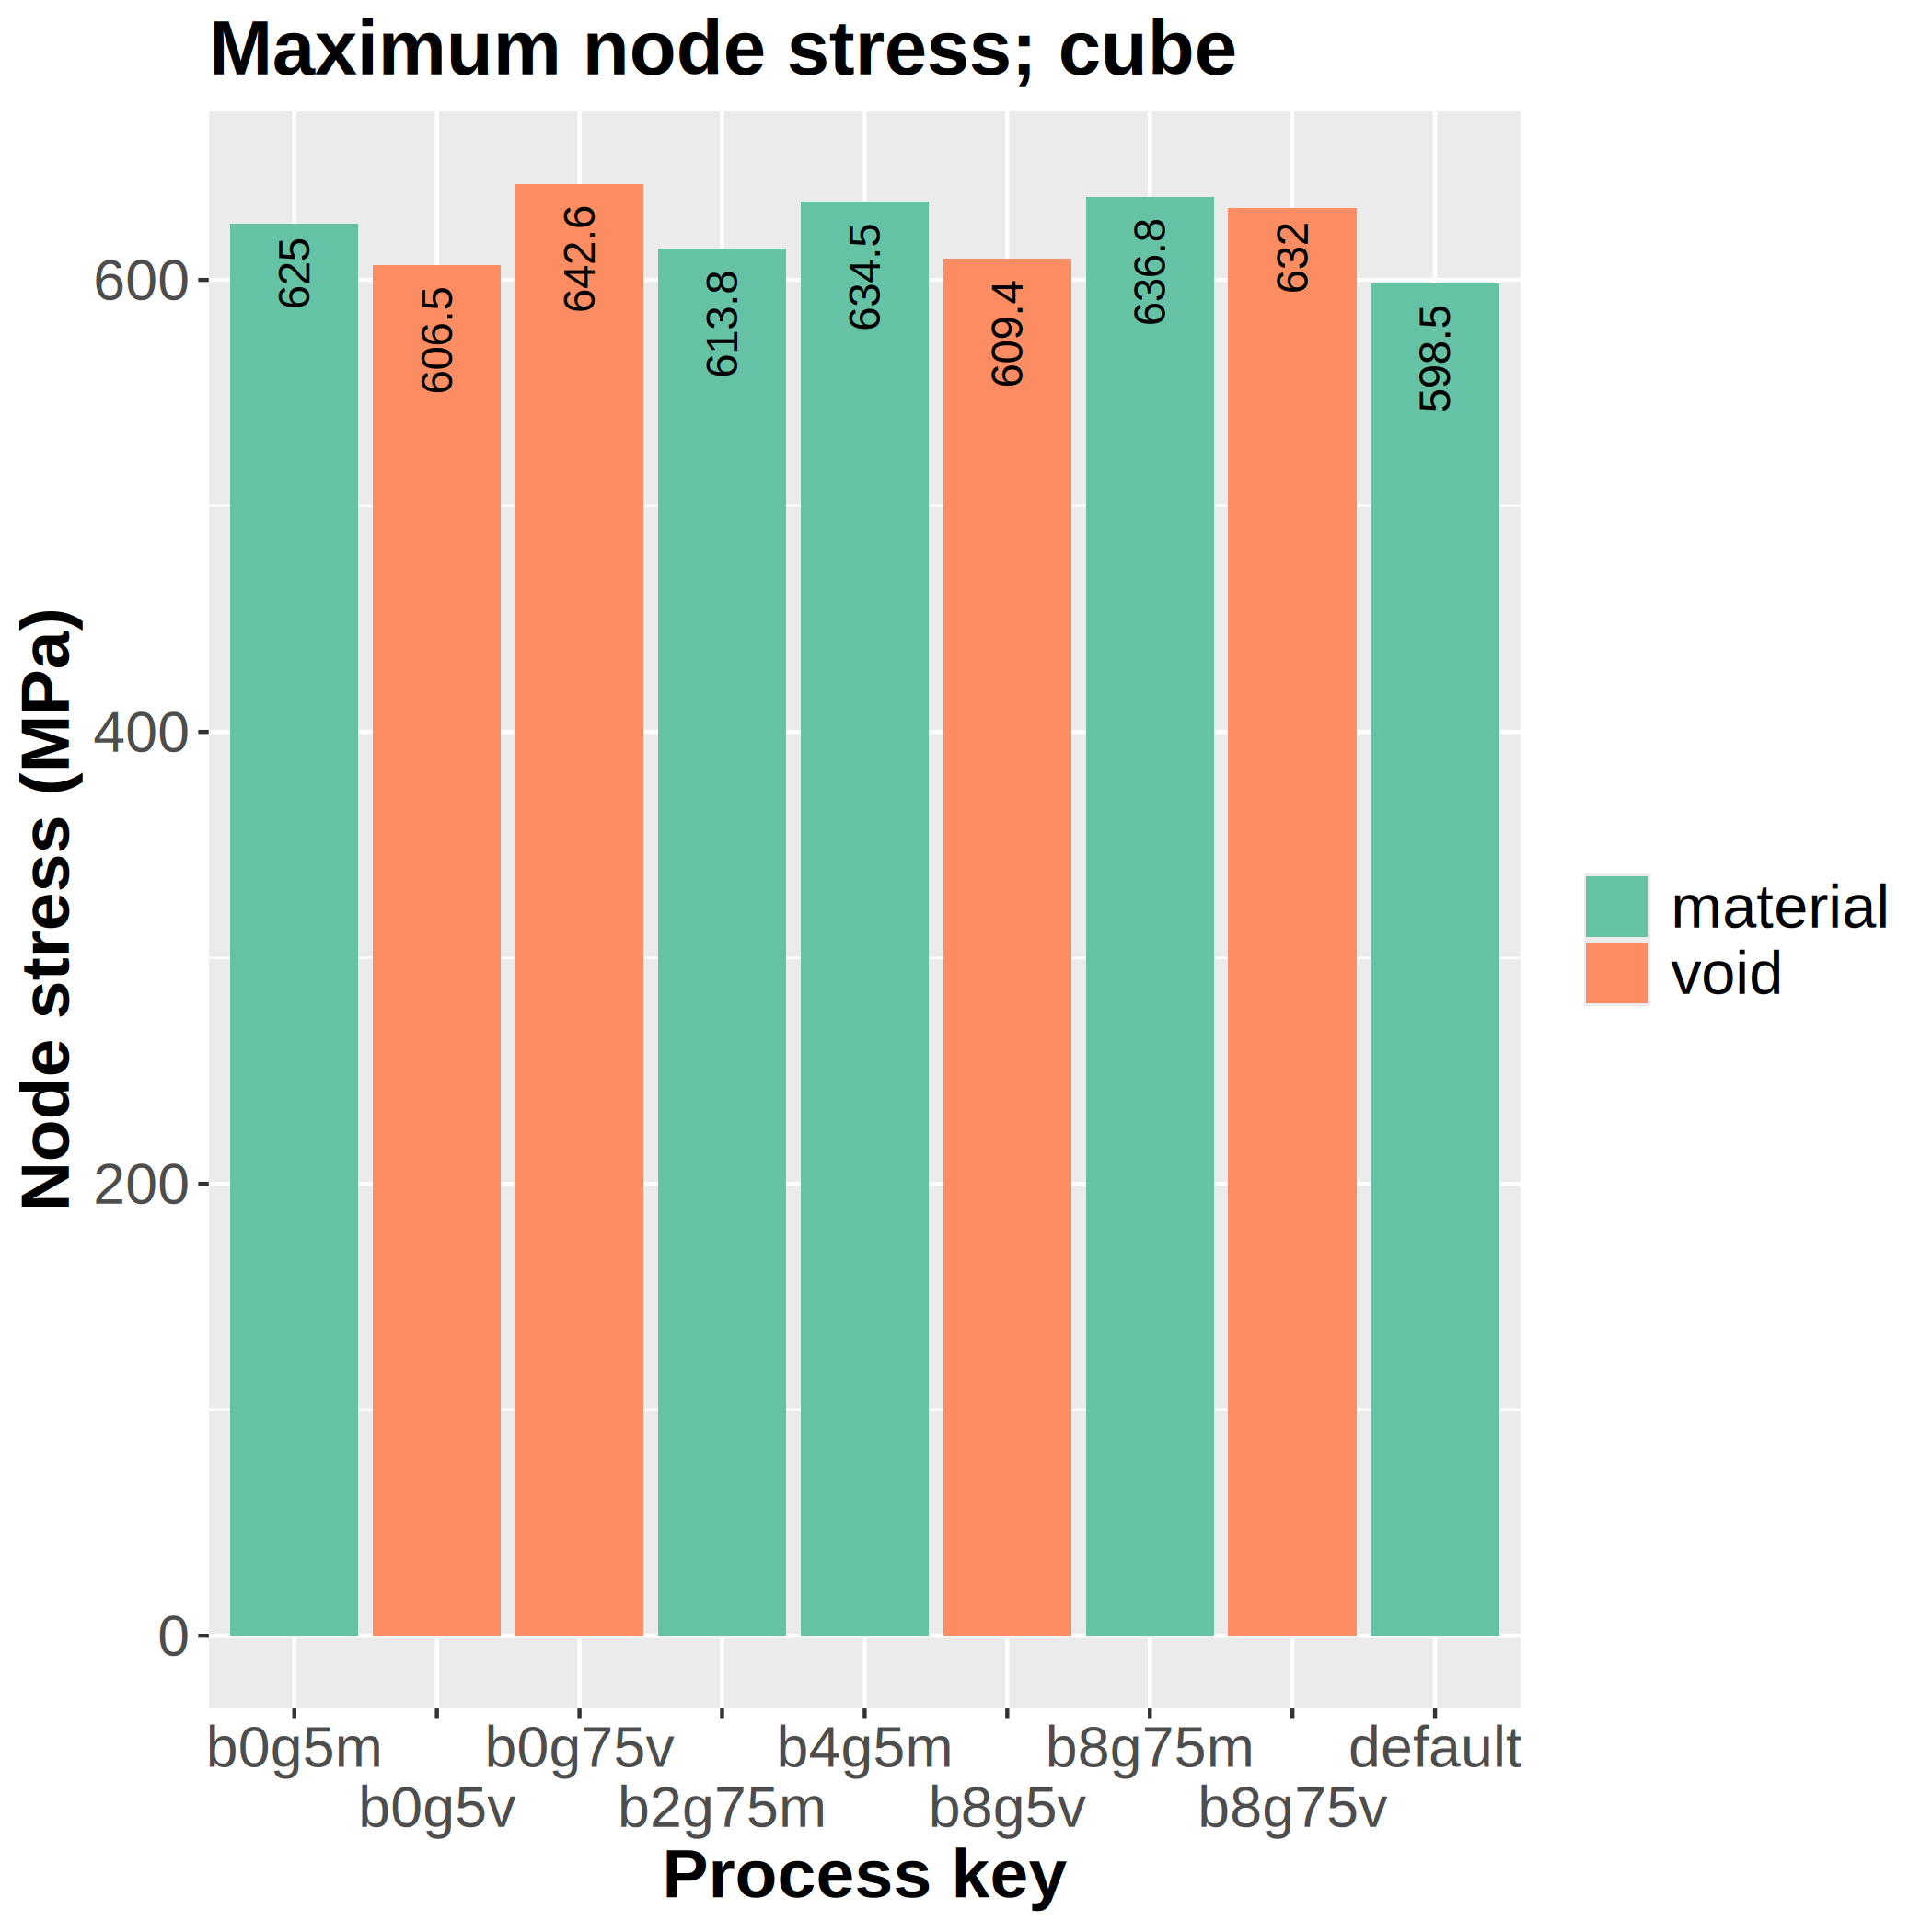
\includegraphics[width=\textwidth]{cube _stressmax3.png}
    \label{}
  \end{subfigure}
  \caption{Results of cube.}
  \label{fig:cuberesults}
\end{figure}

\begin{figure}[h!]
  \centering 
  \begin{subfigure}[b]{0.45\textwidth}
    \centering 
    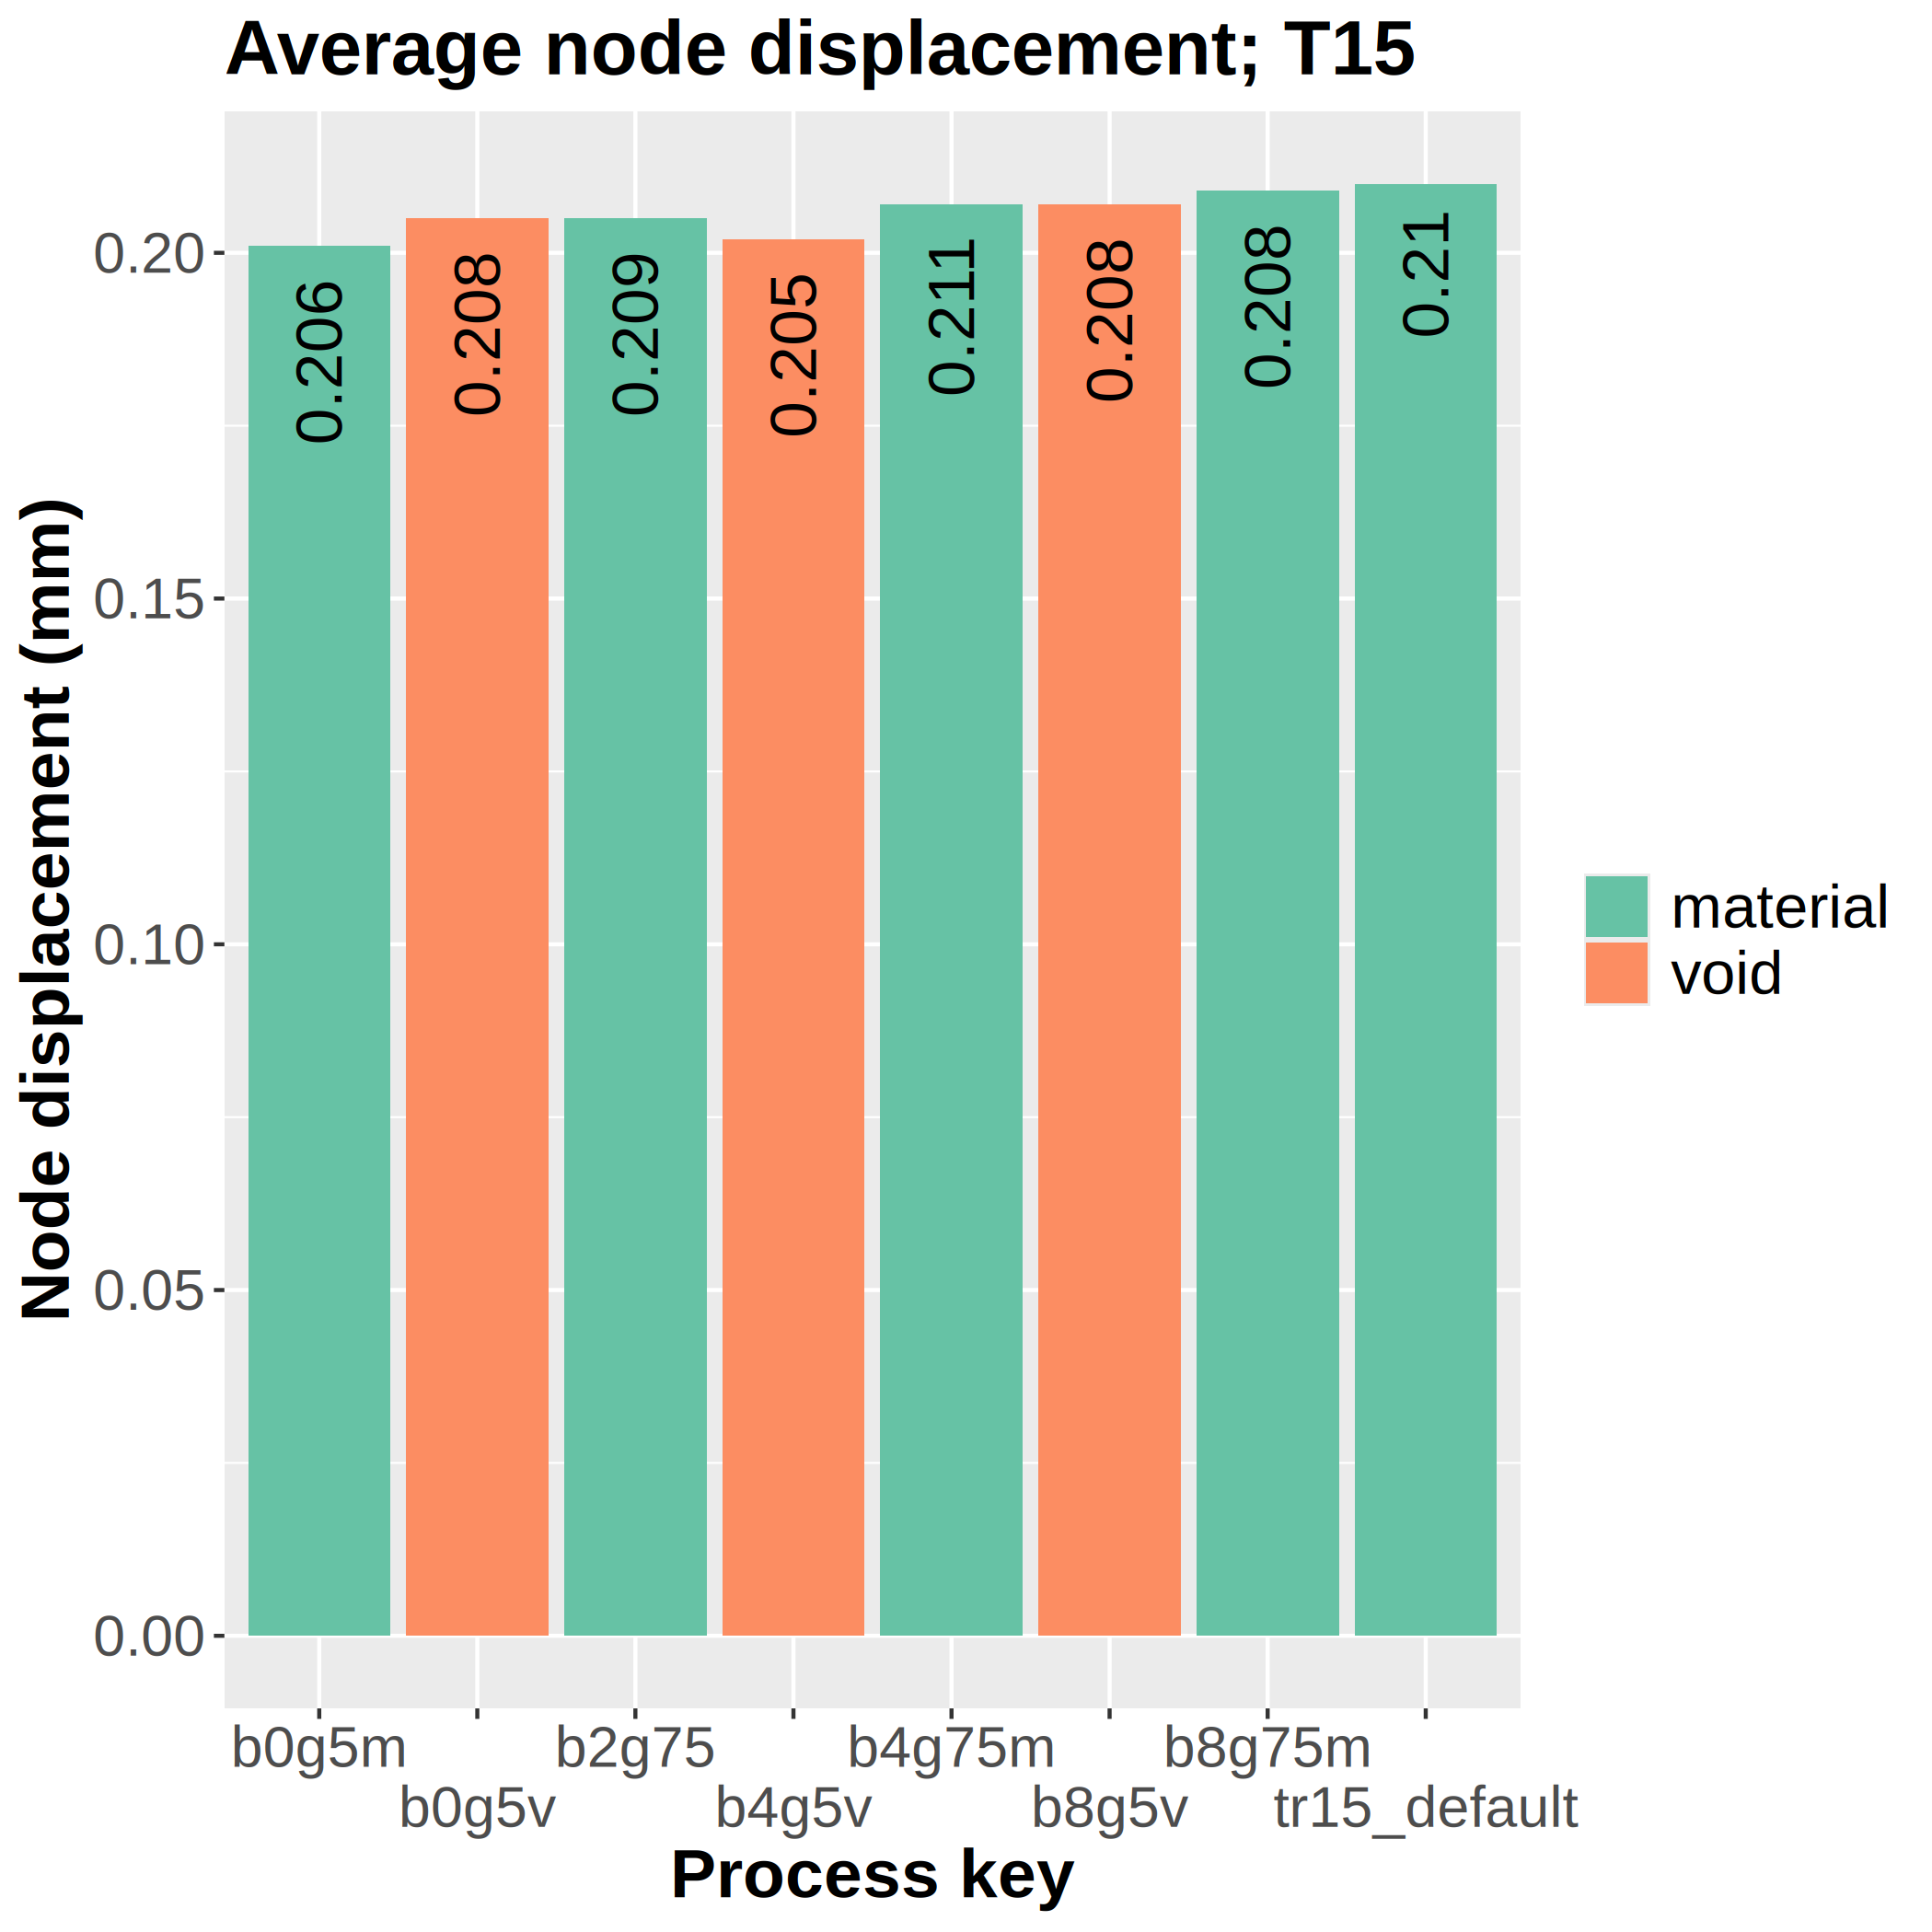
\includegraphics[width=\textwidth]{T15 _disp3.png}
    \label{}
  \end{subfigure}
  \begin{subfigure}[b]{0.45\textwidth}
    \centering 
    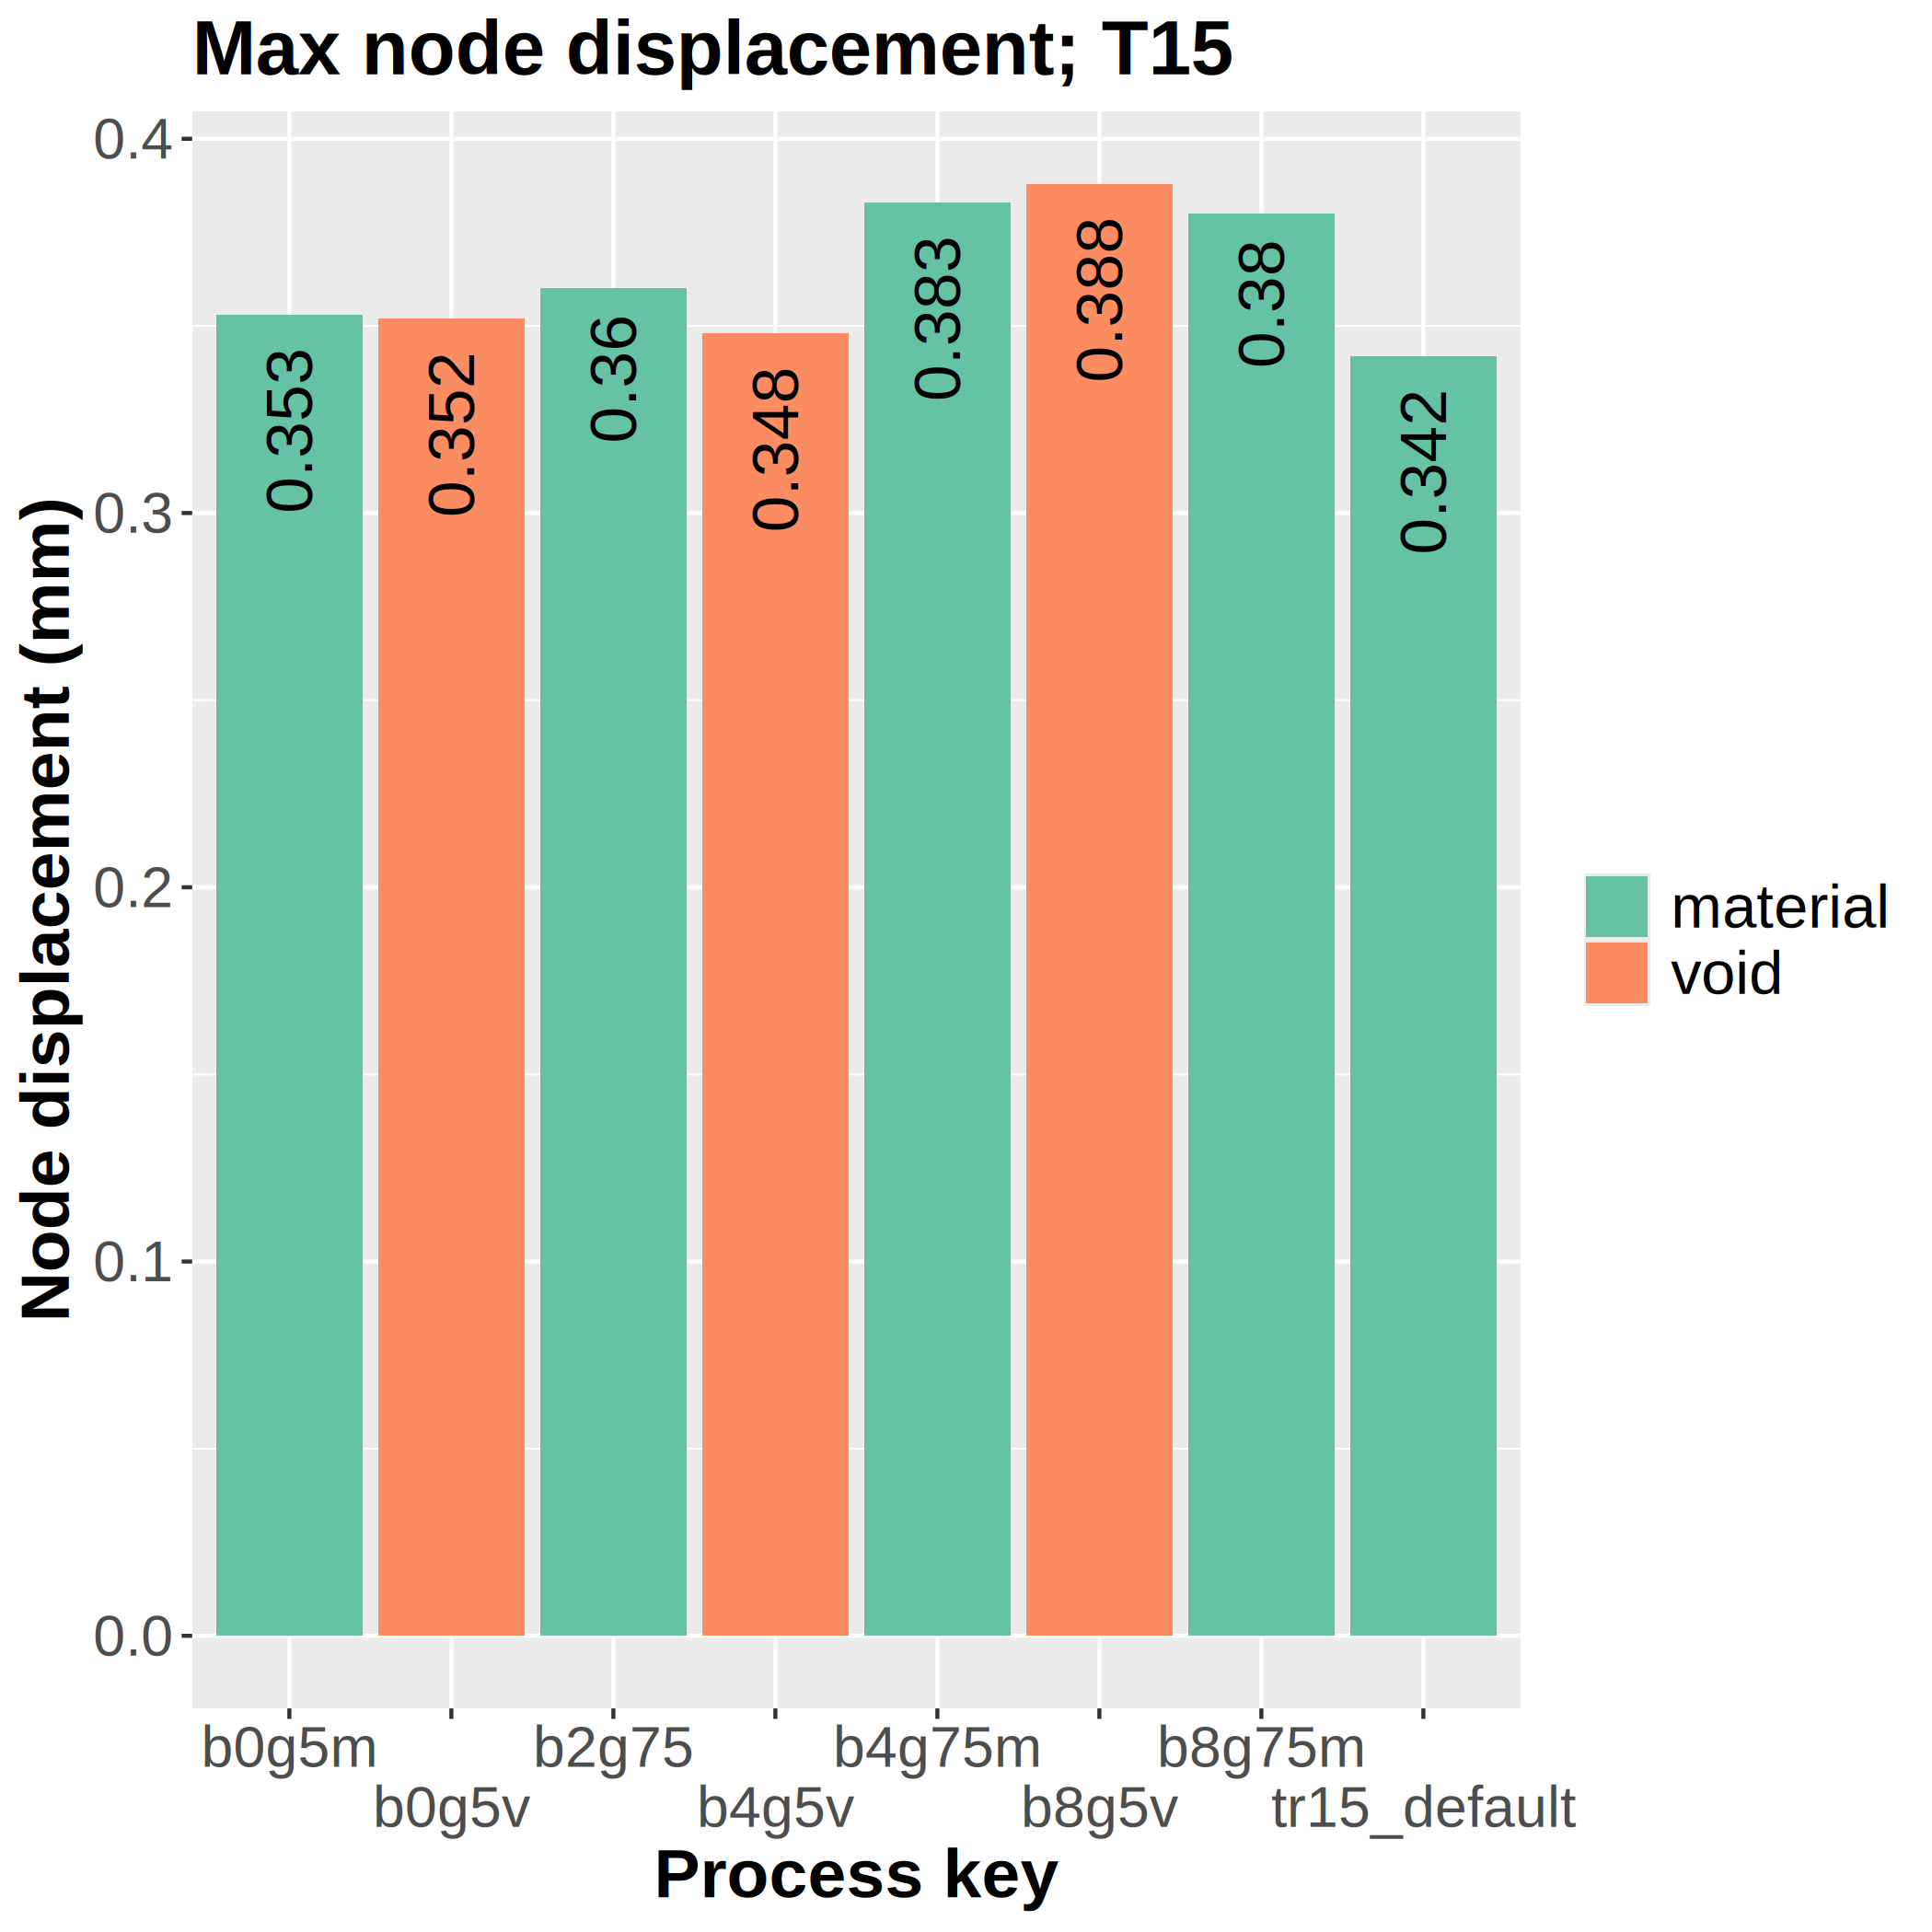
\includegraphics[width=\textwidth]{T15 _dispmax3.png}
    \label{}
  \end{subfigure}
  \begin{subfigure}[b]{0.45\textwidth}
    \centering 
    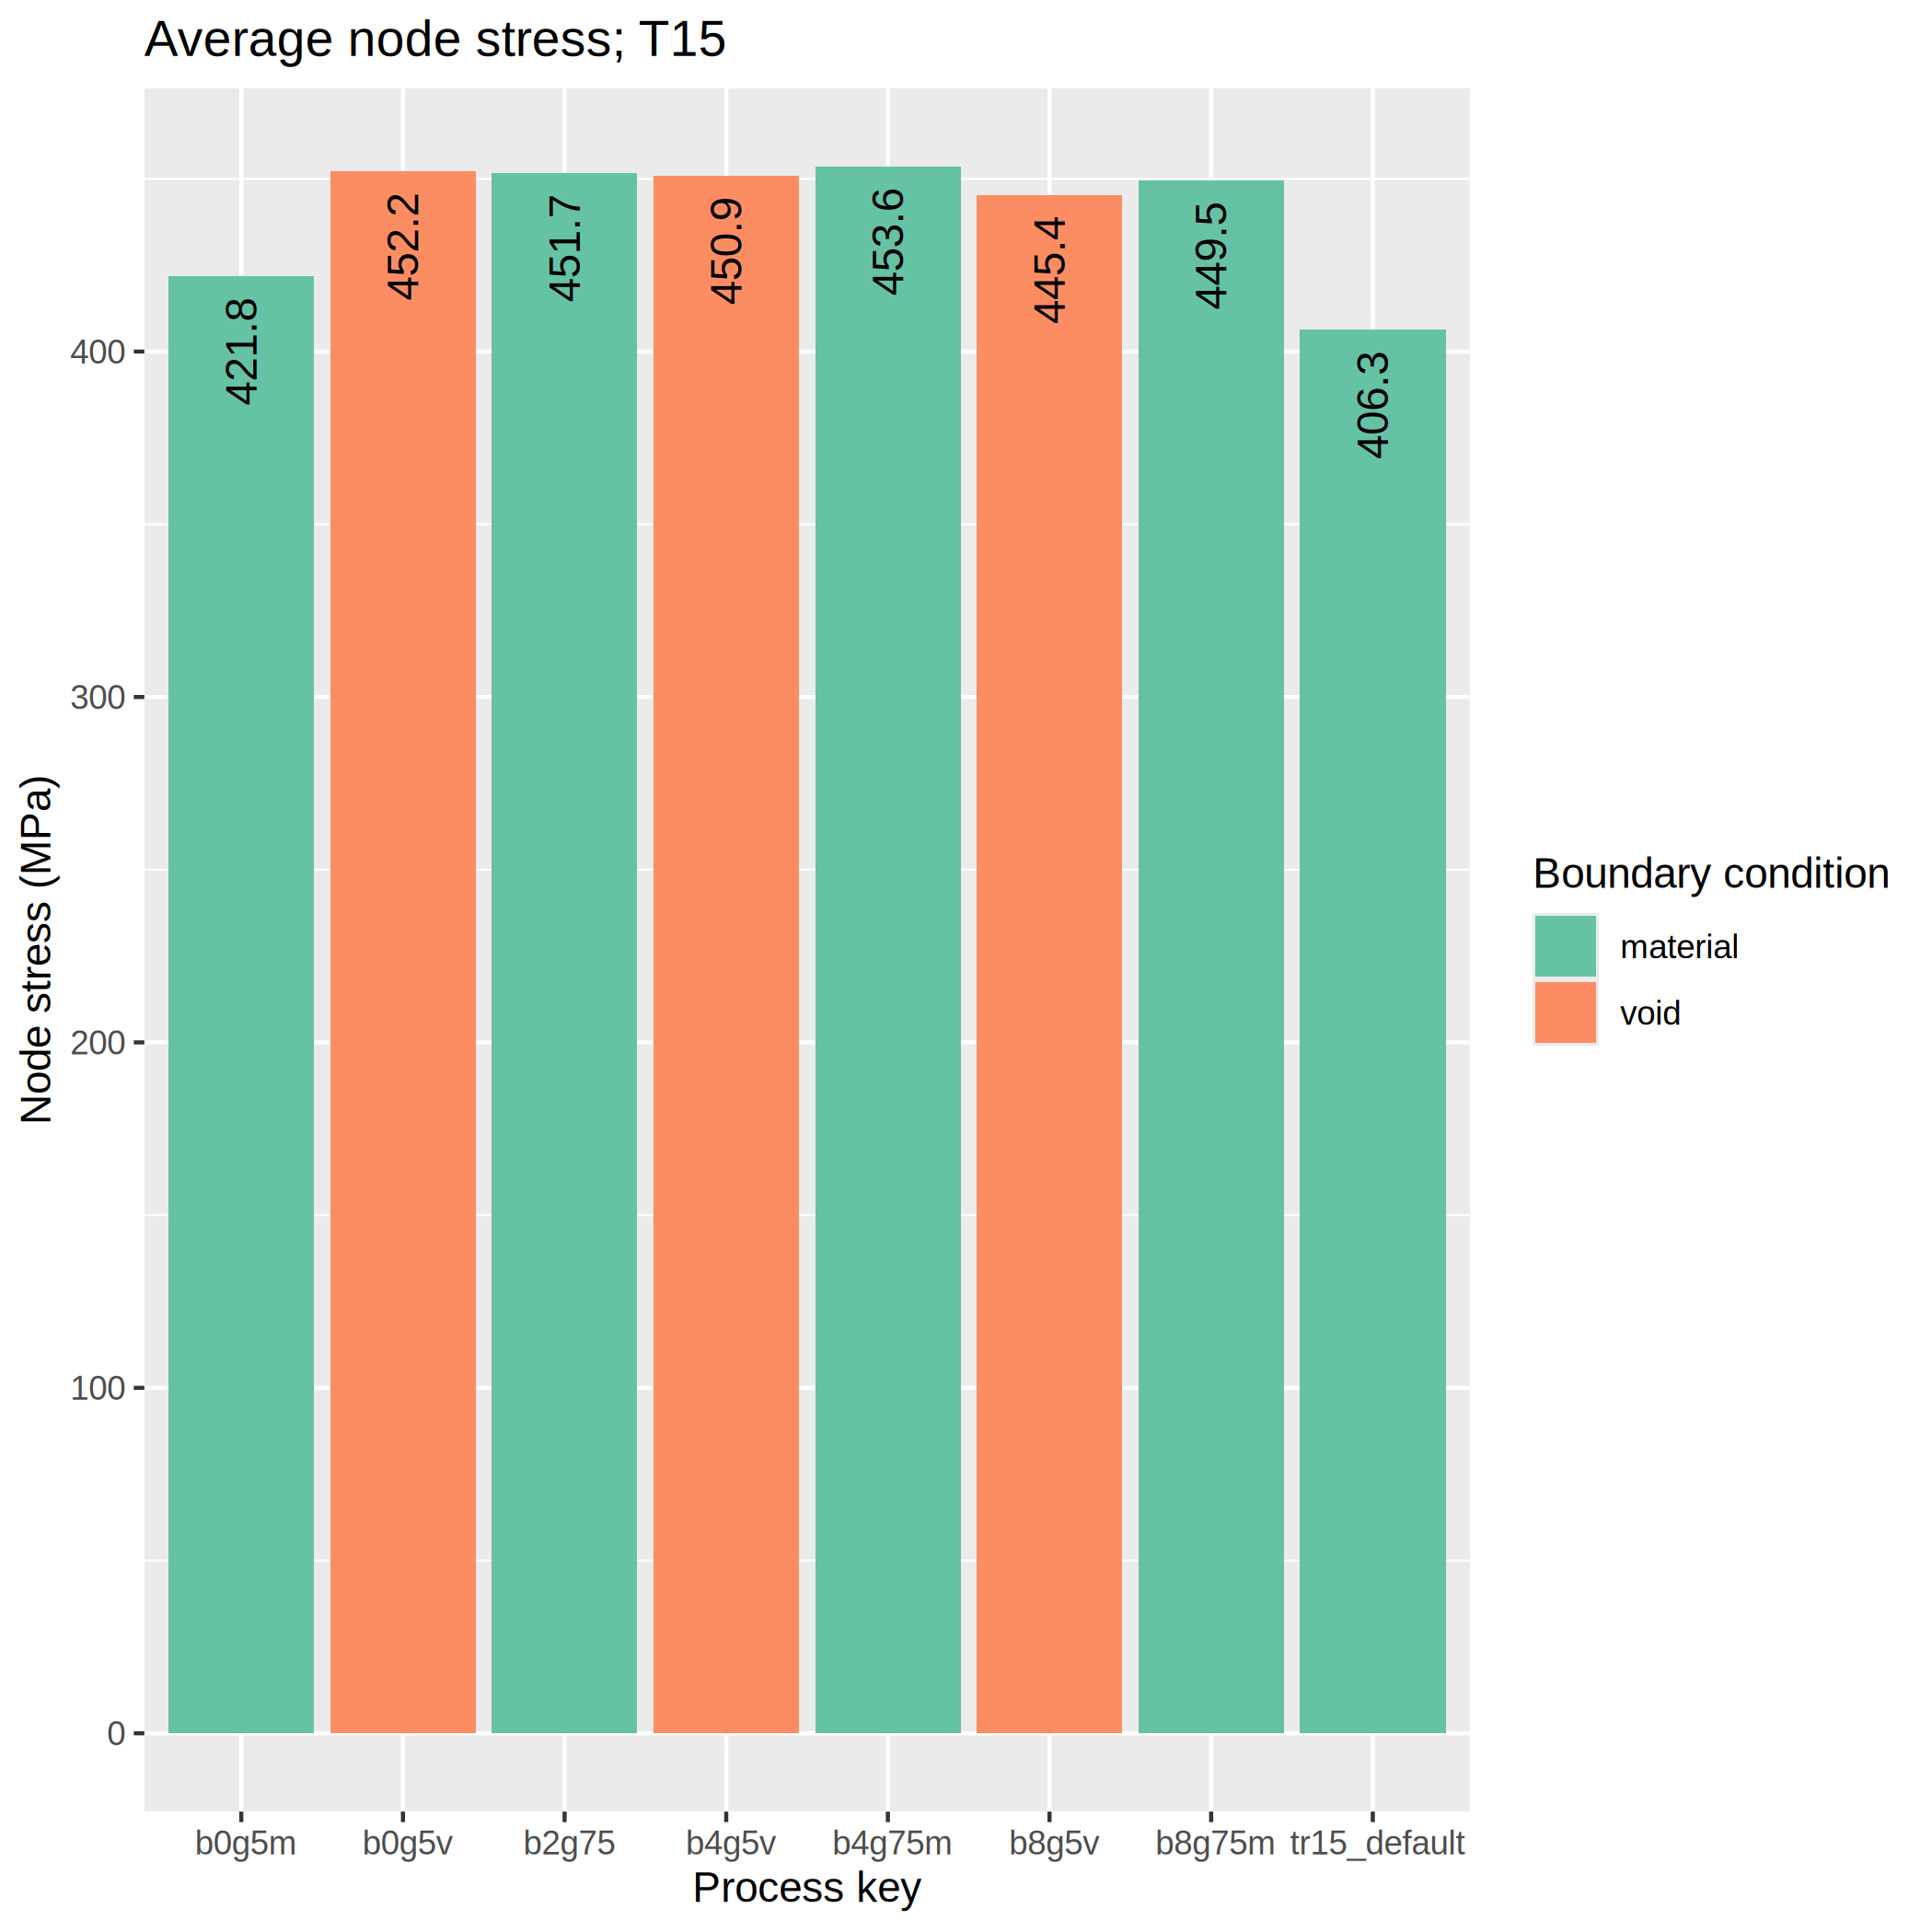
\includegraphics[width=\textwidth]{T15 _stress3.png}
    \label{}
  \end{subfigure}
  \begin{subfigure}[b]{0.45\textwidth}
    \centering 
    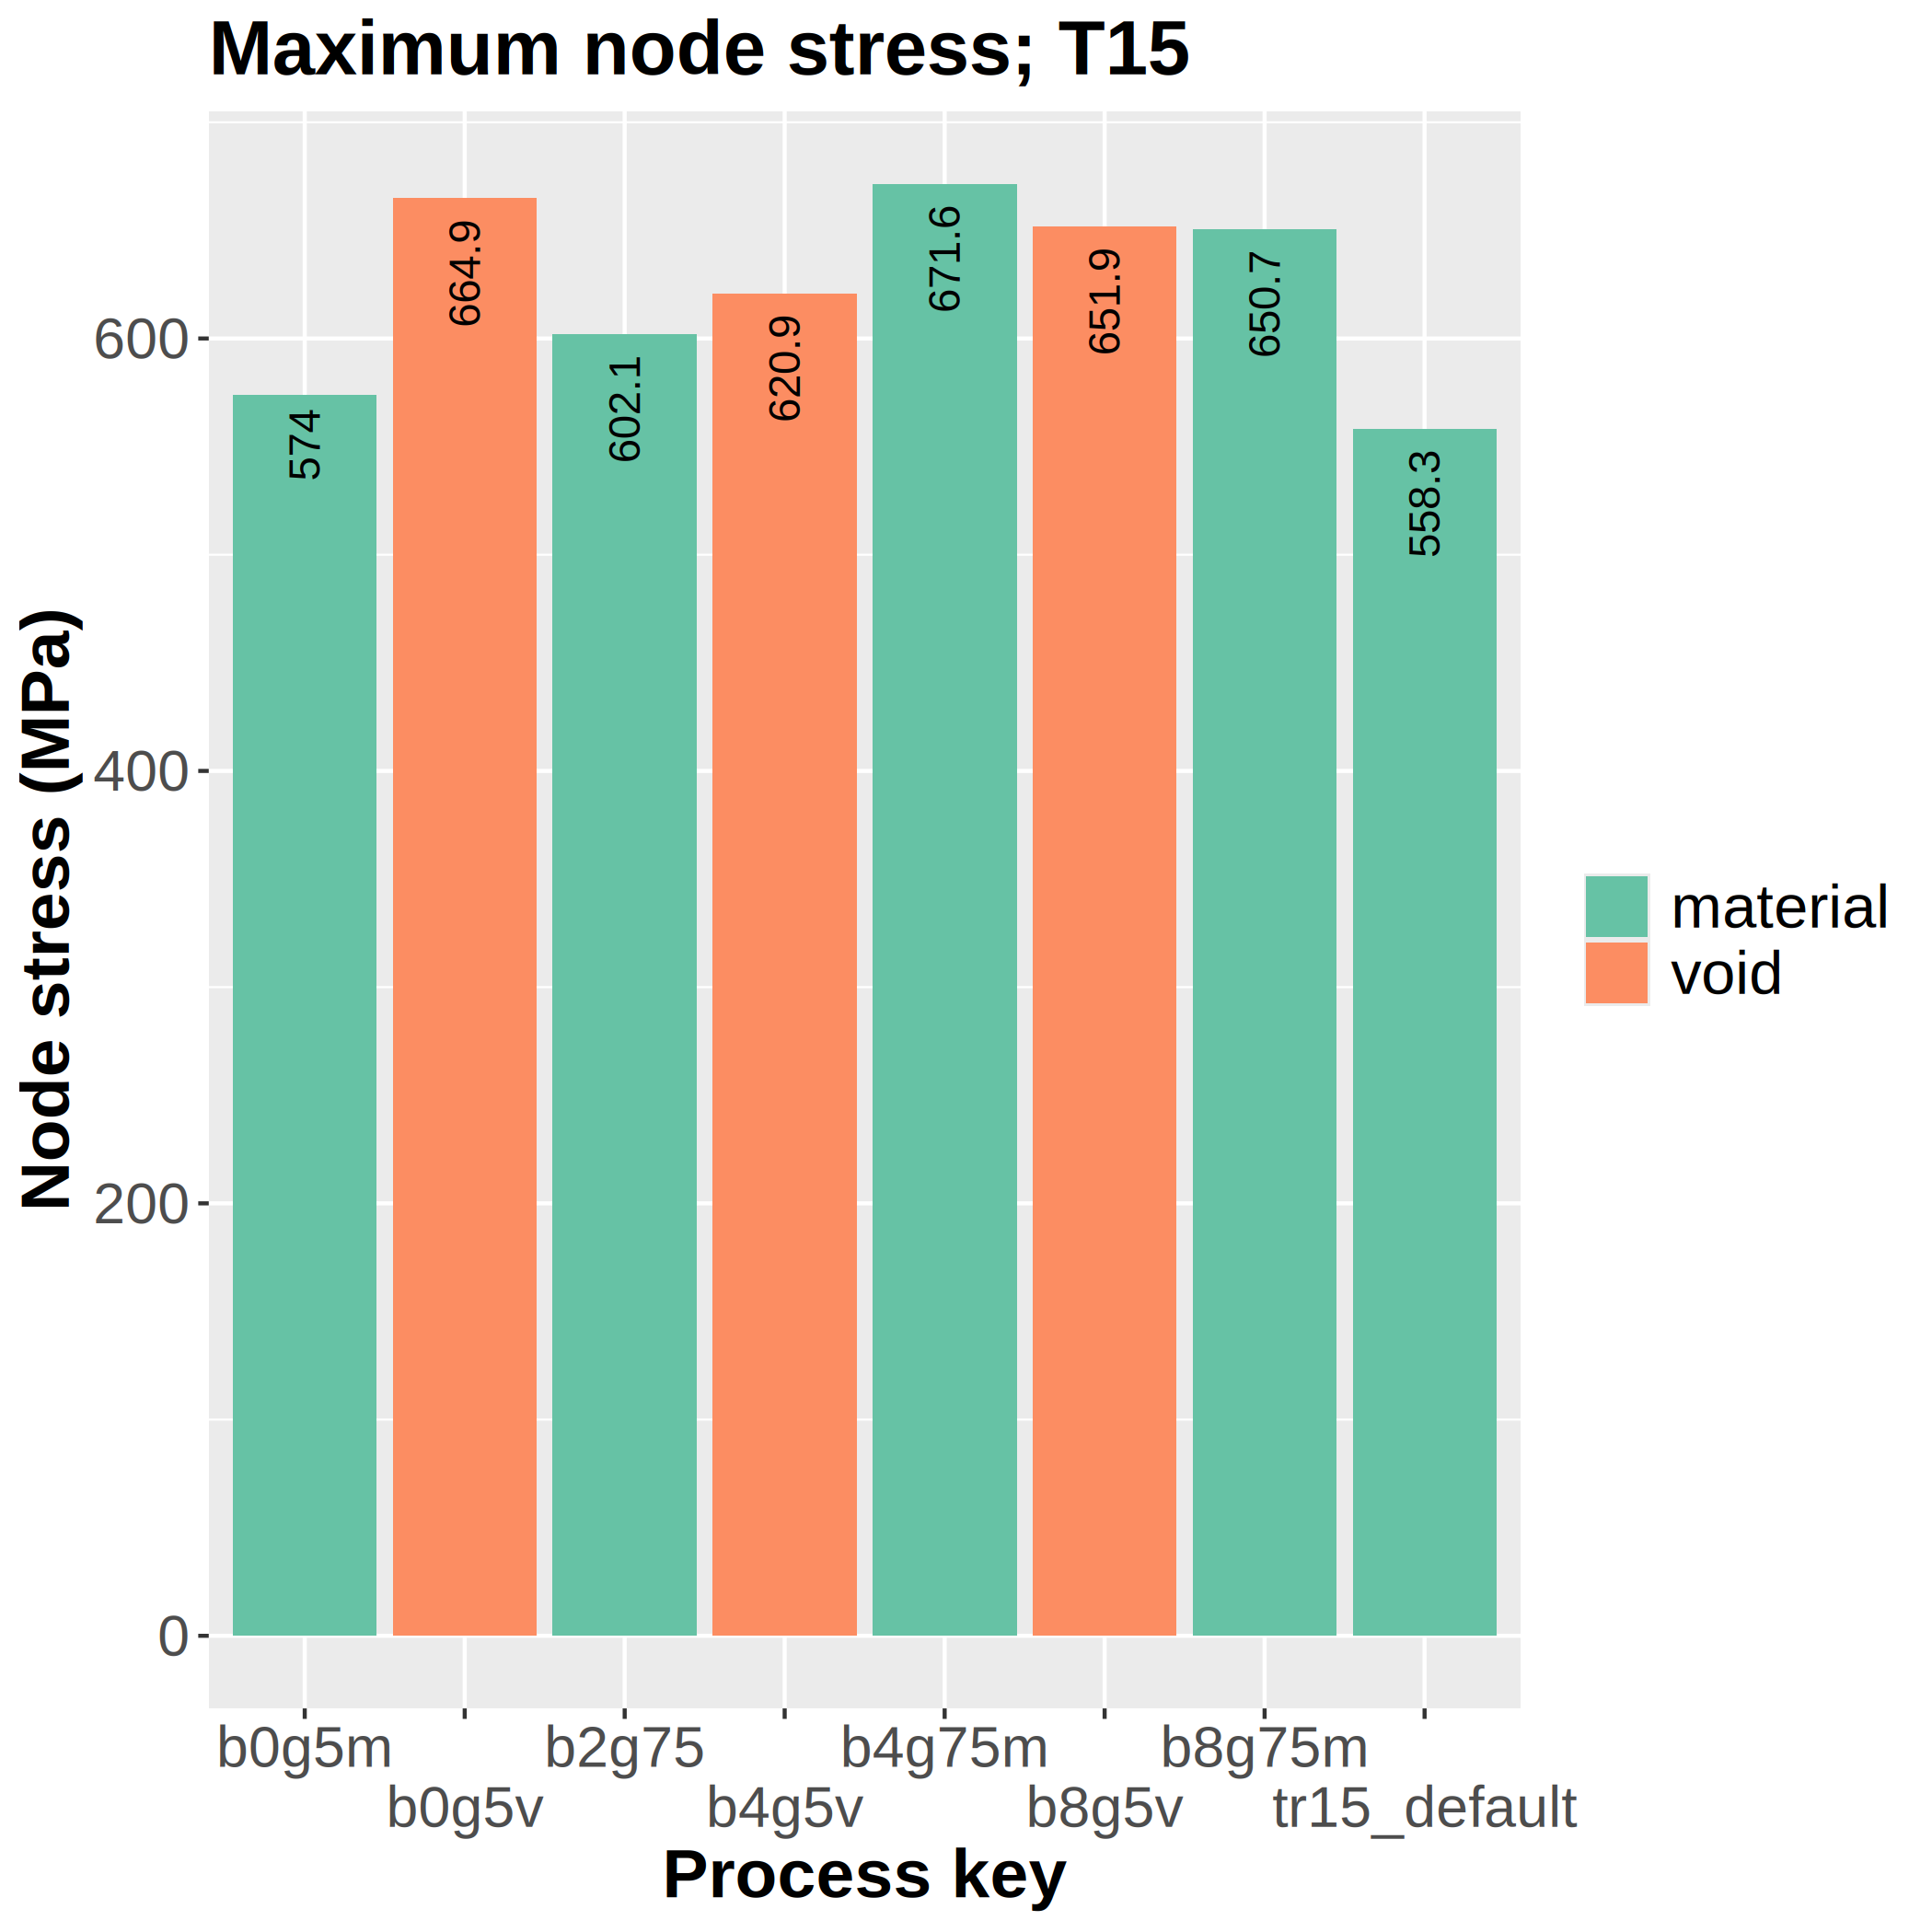
\includegraphics[width=\textwidth]{T15 _stressmax3.png}
    \label{}
  \end{subfigure}
  \caption{Results of 15\degree triangle.}
  \label{fig:tri15_results}
\end{figure}

\begin{figure}
  \centering 
  \begin{subfigure}[b]{0.45\textwidth}
    \centering 
    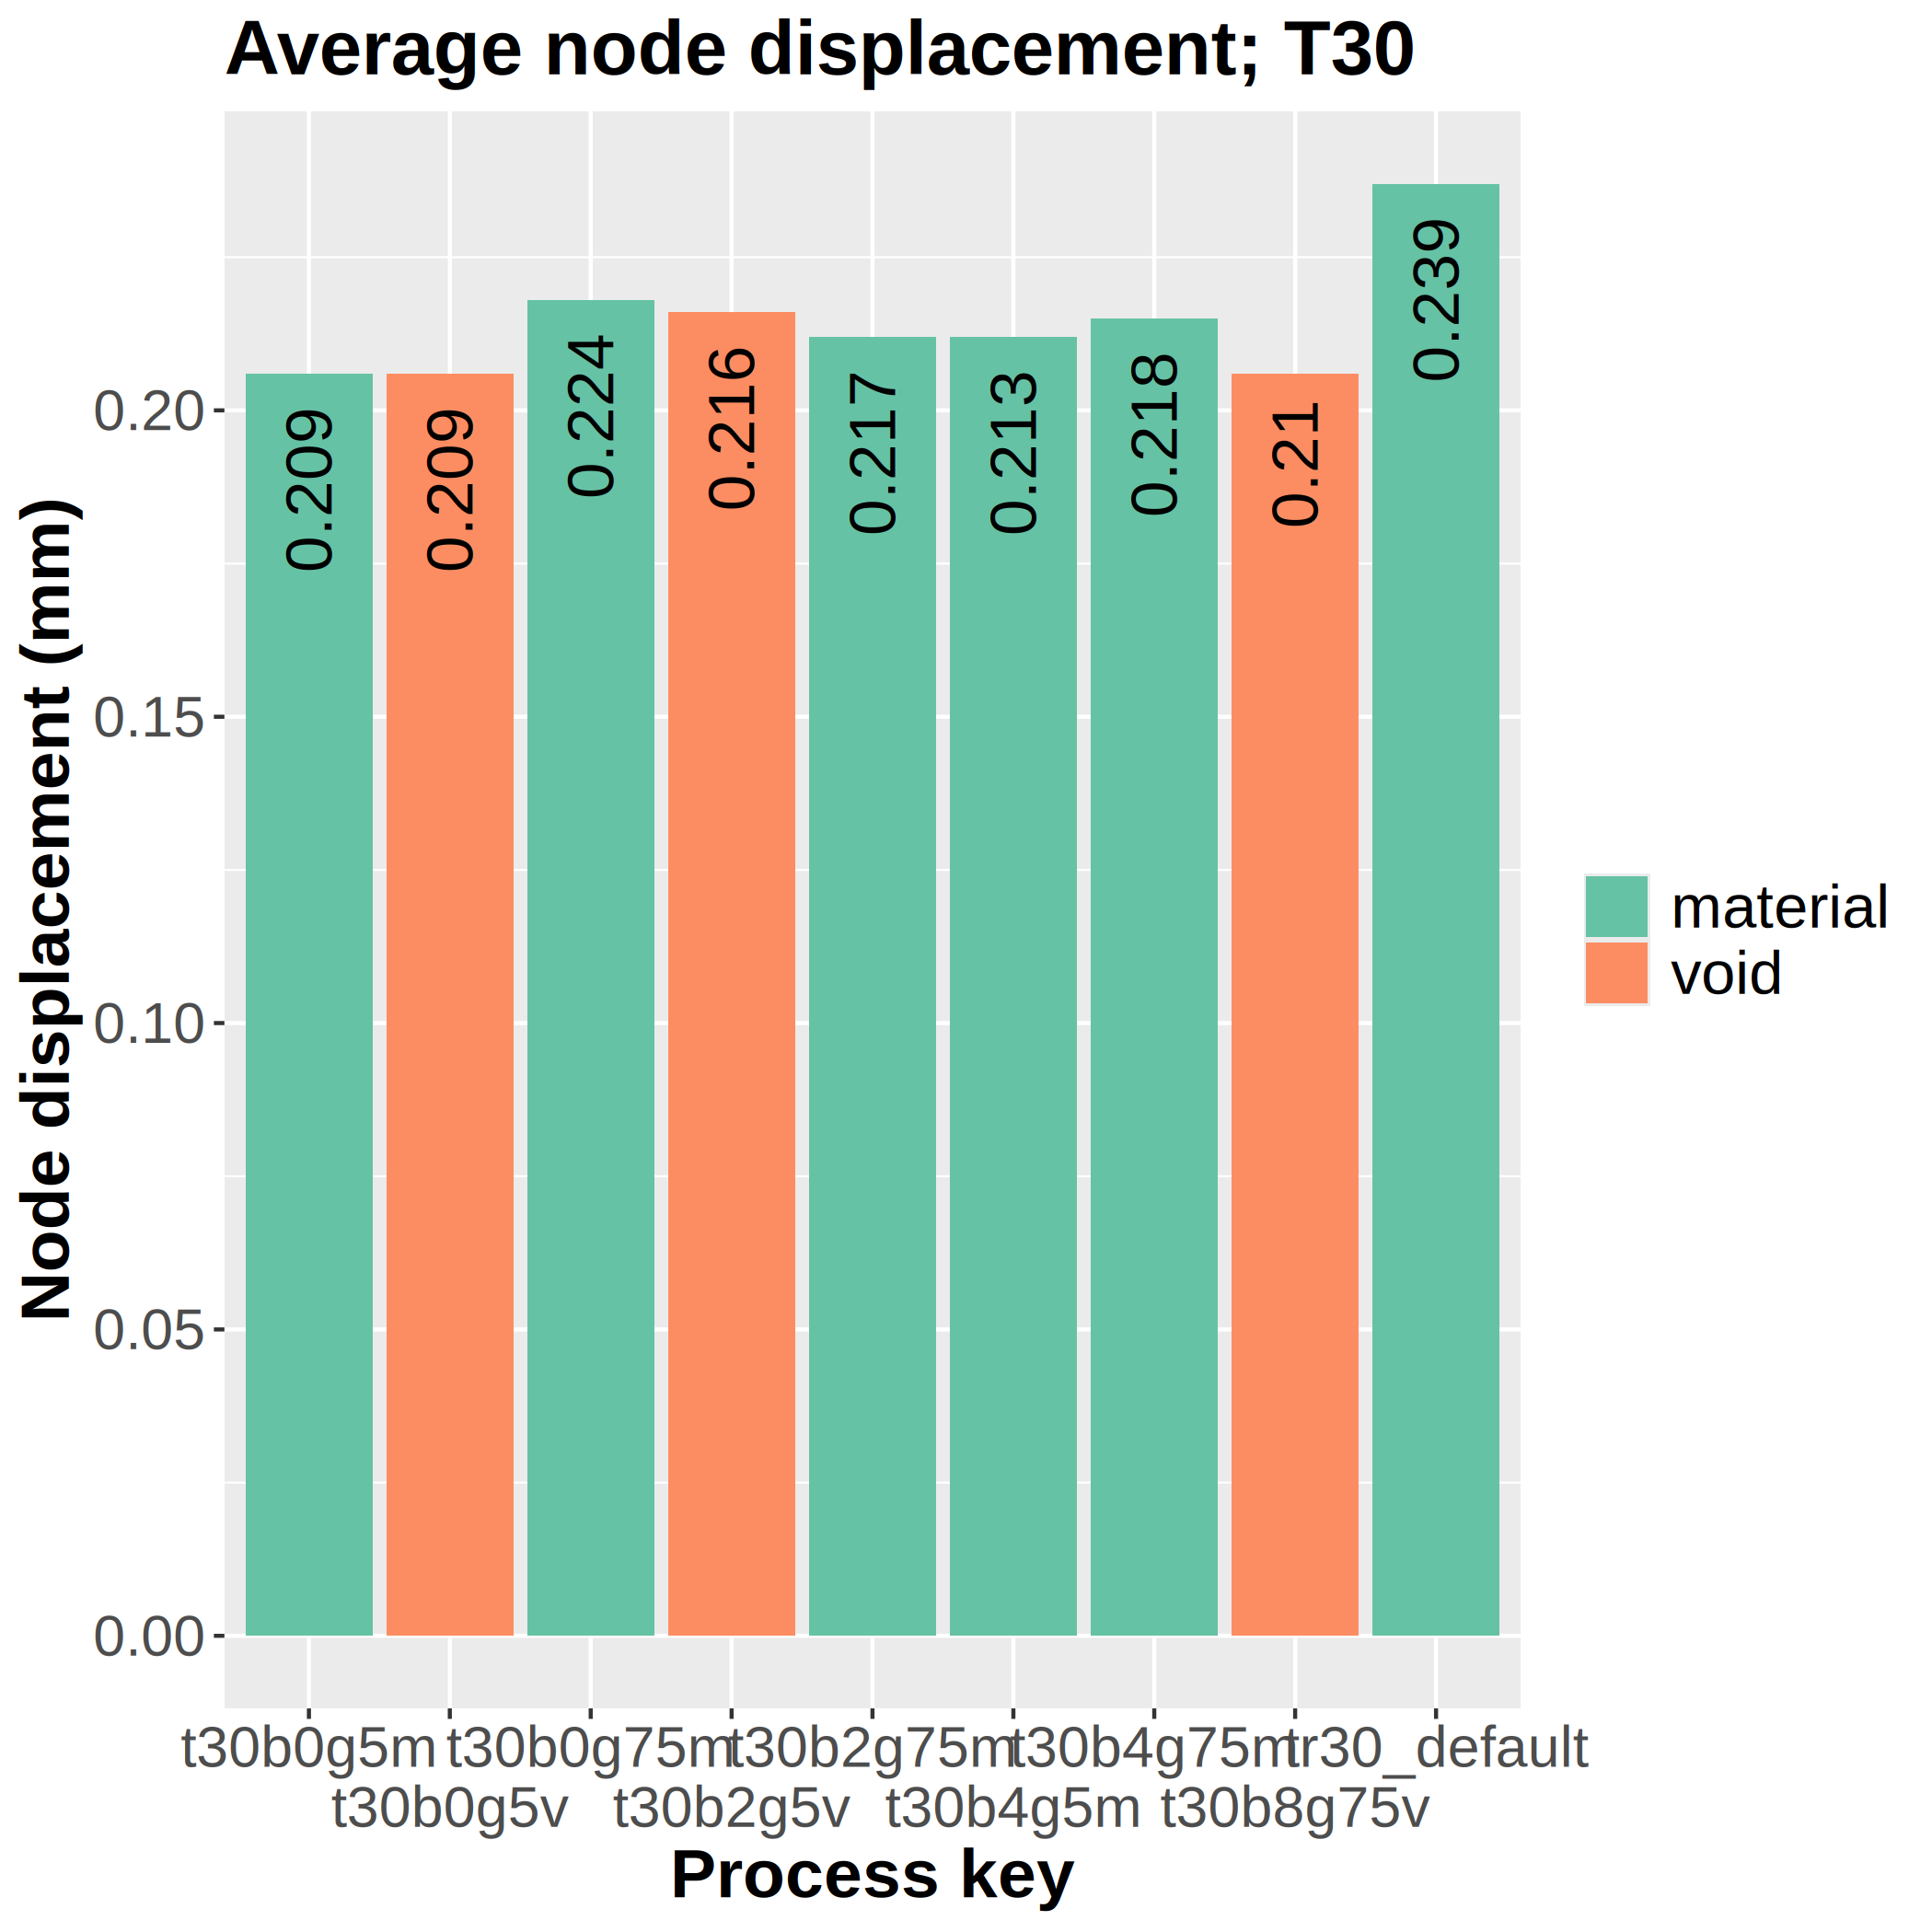
\includegraphics[width=\textwidth]{T30 _disp3.png}
    \label{}
  \end{subfigure}
  \begin{subfigure}[b]{0.45\textwidth}
    \centering 
    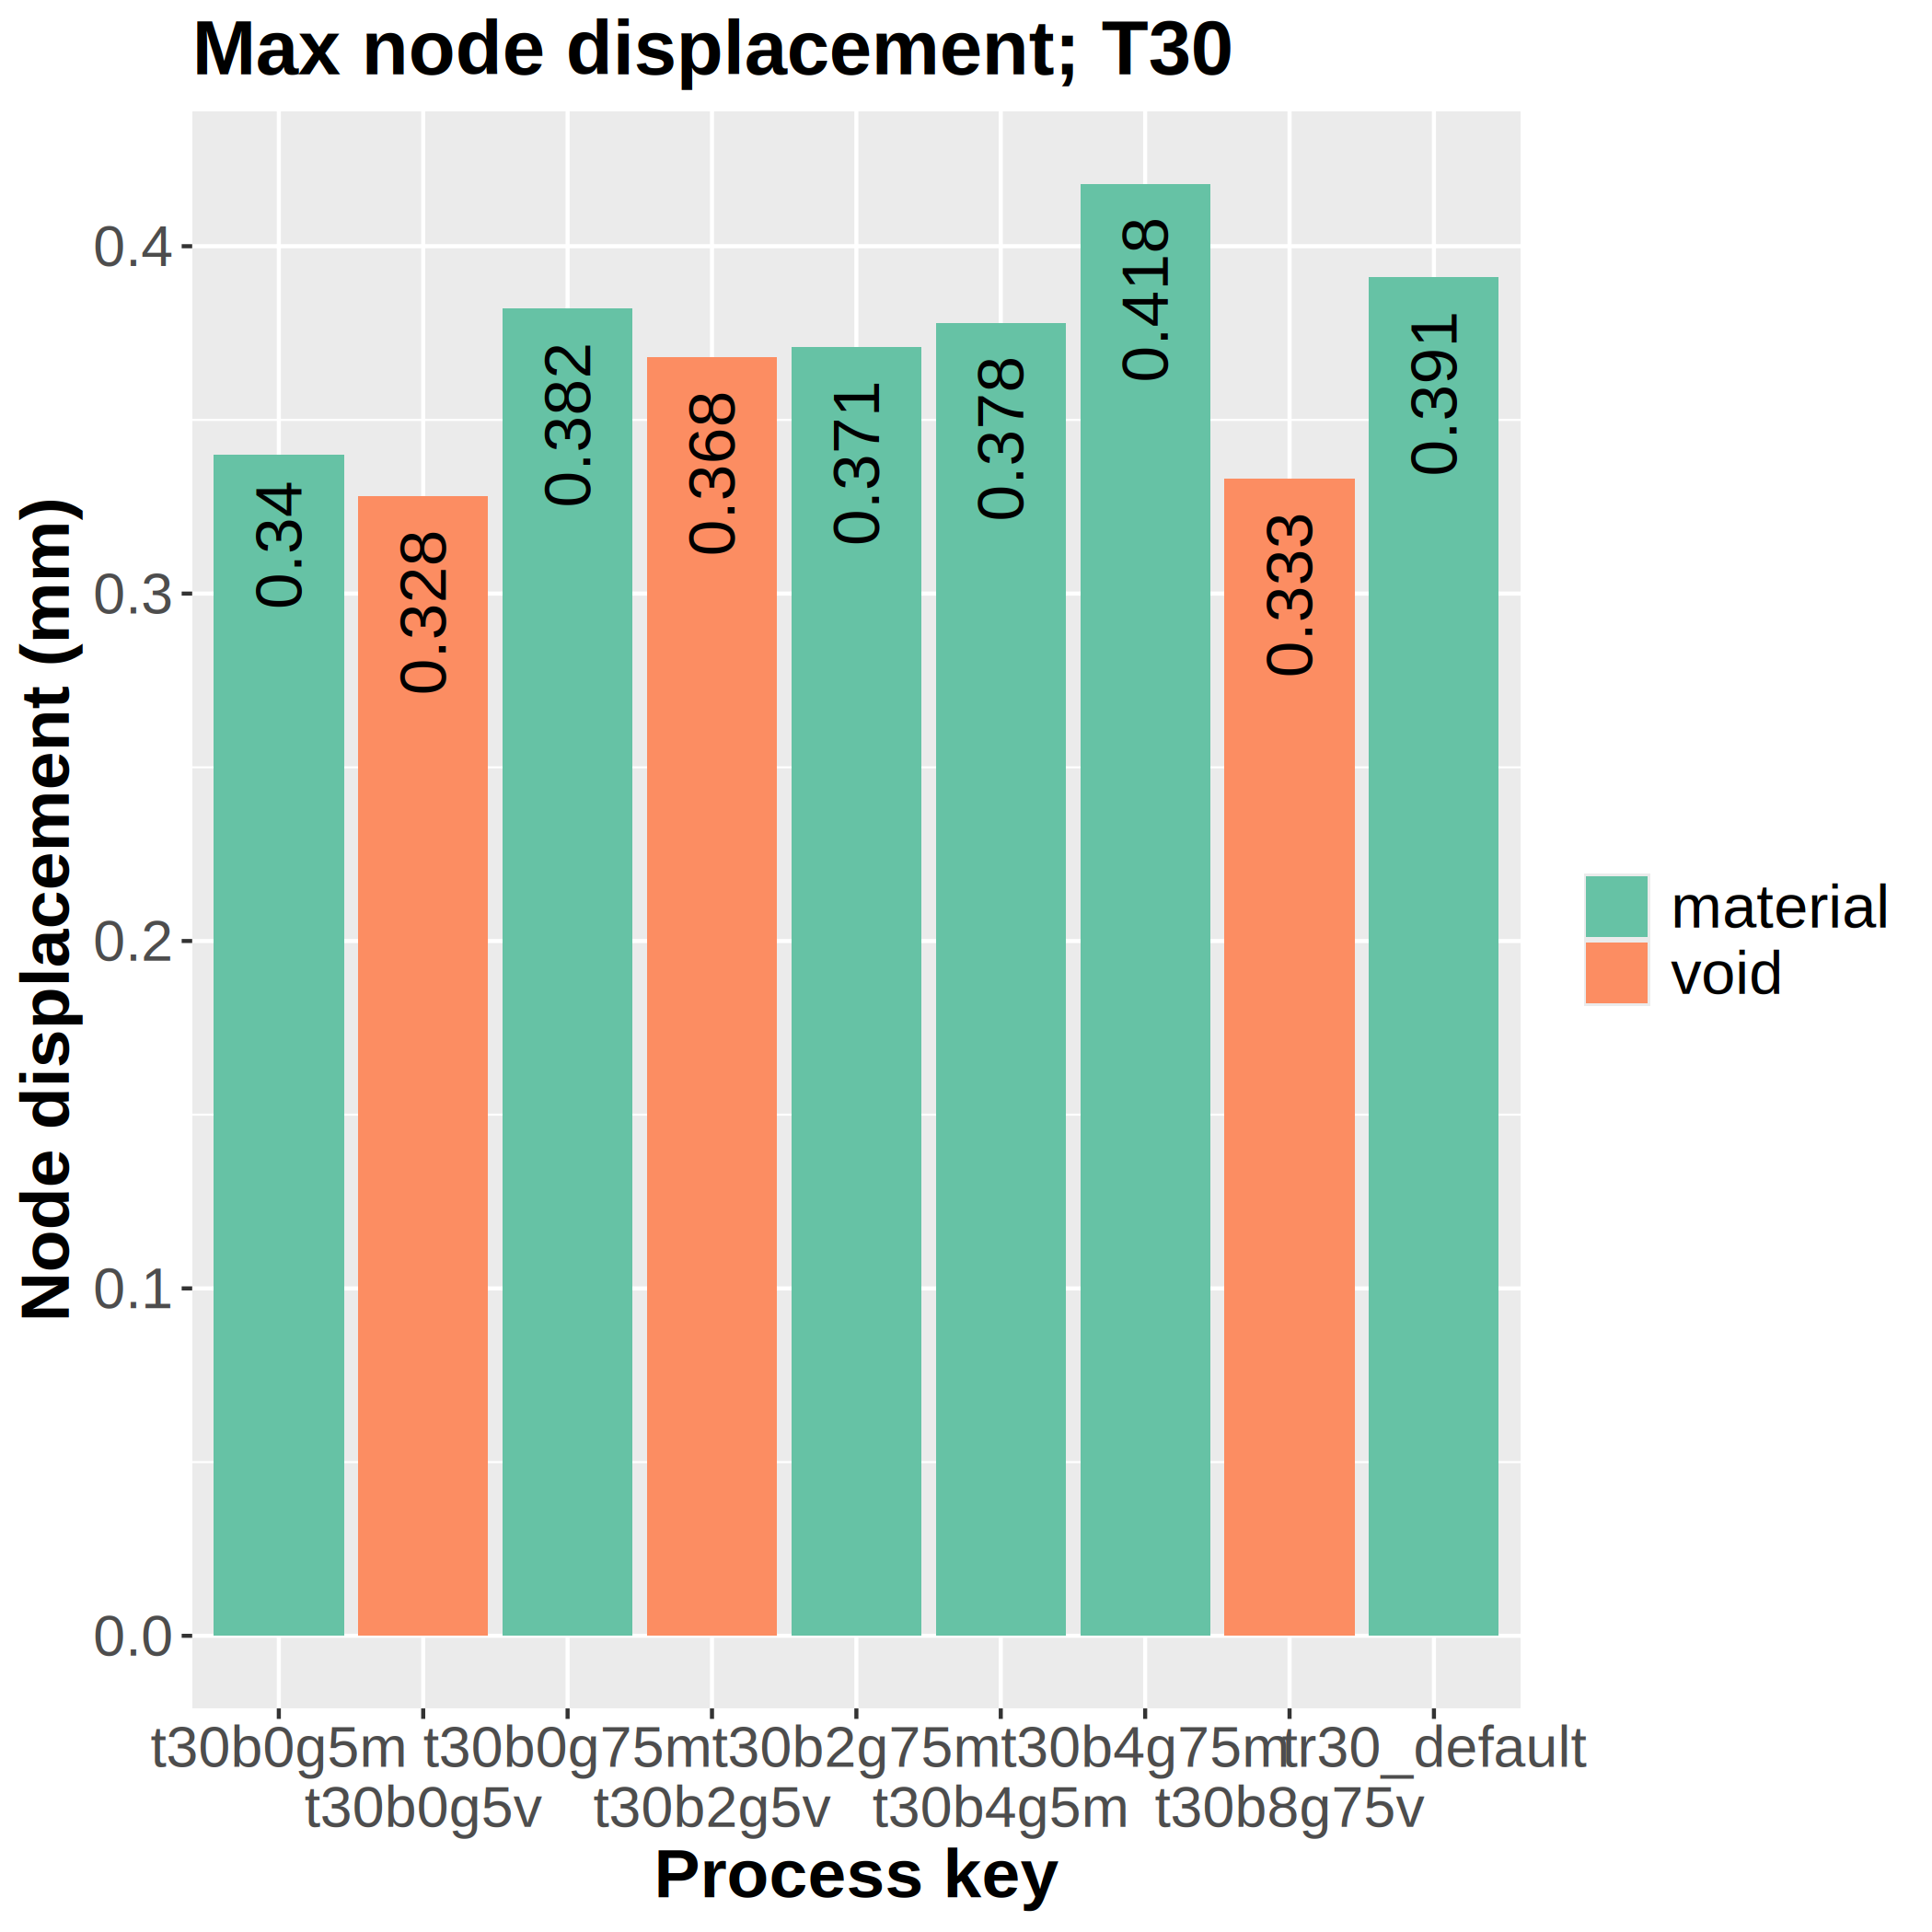
\includegraphics[width=\textwidth]{T30 _dispmax3.png}
    \label{}
  \end{subfigure}
  \begin{subfigure}[b]{0.45\textwidth}
    \centering 
    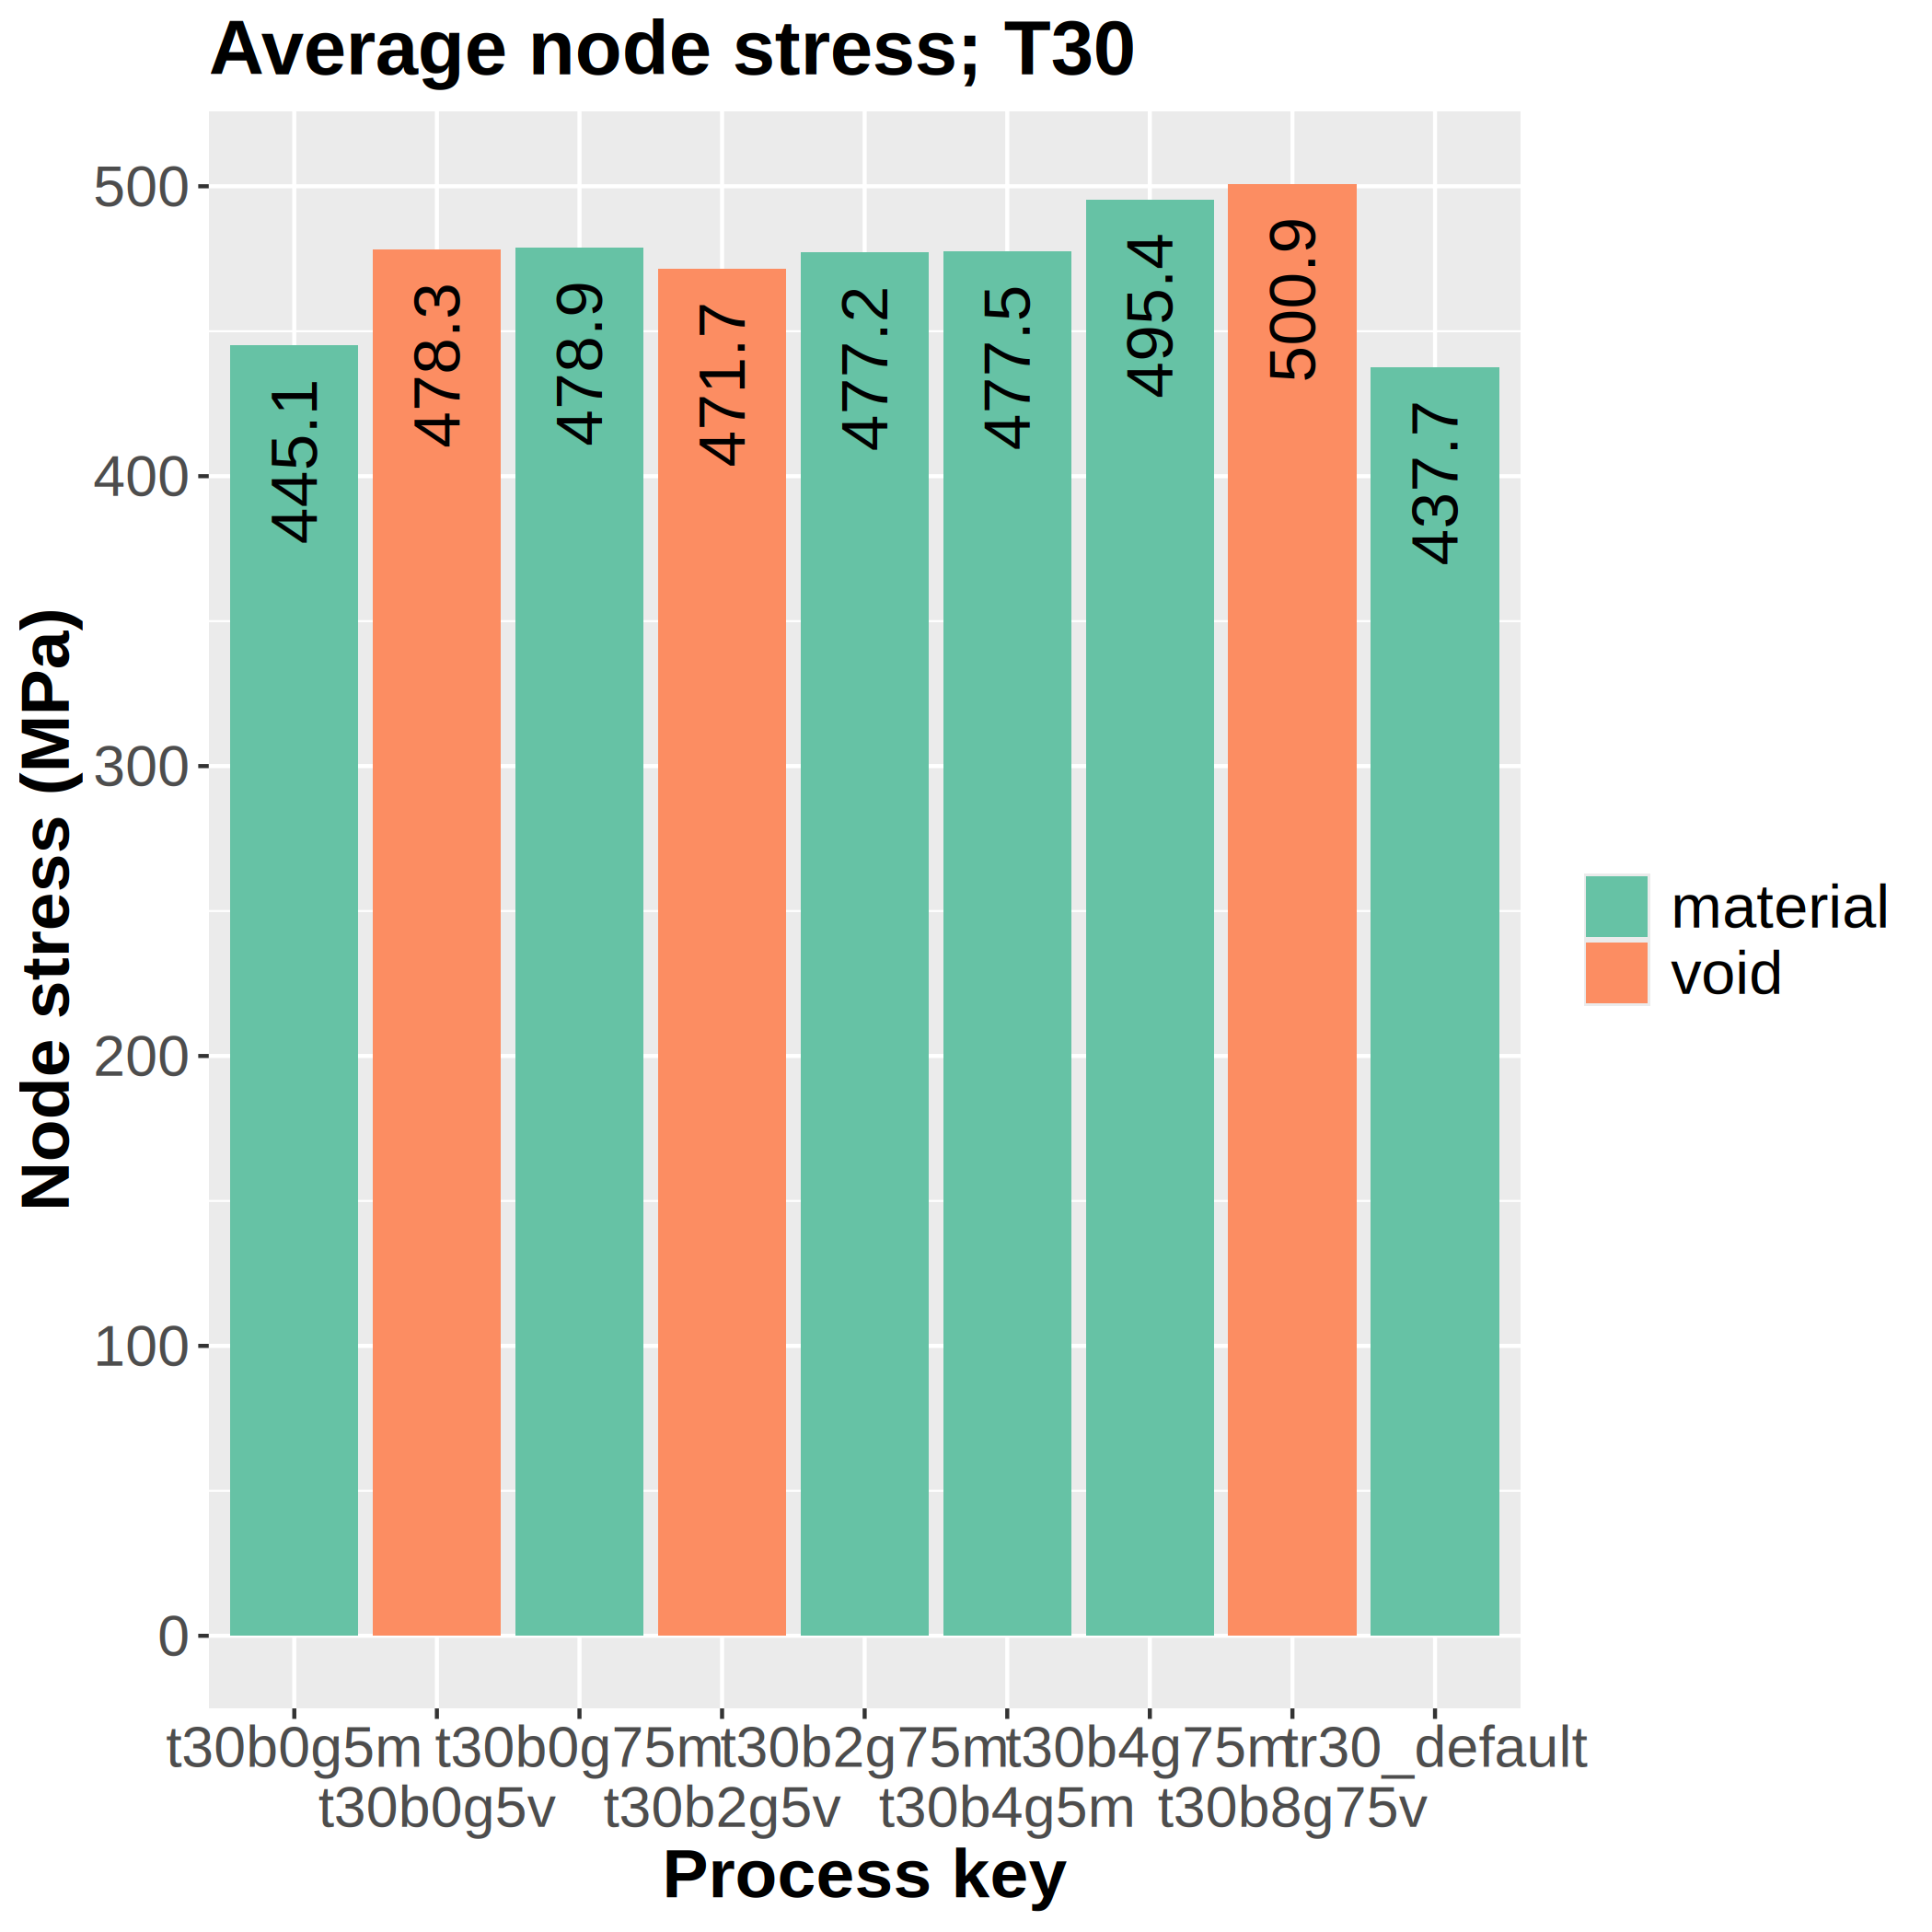
\includegraphics[width=\textwidth]{T30 _stress3.png}
    \label{}
  \end{subfigure}
  \begin{subfigure}[b]{0.45\textwidth}
    \centering 
    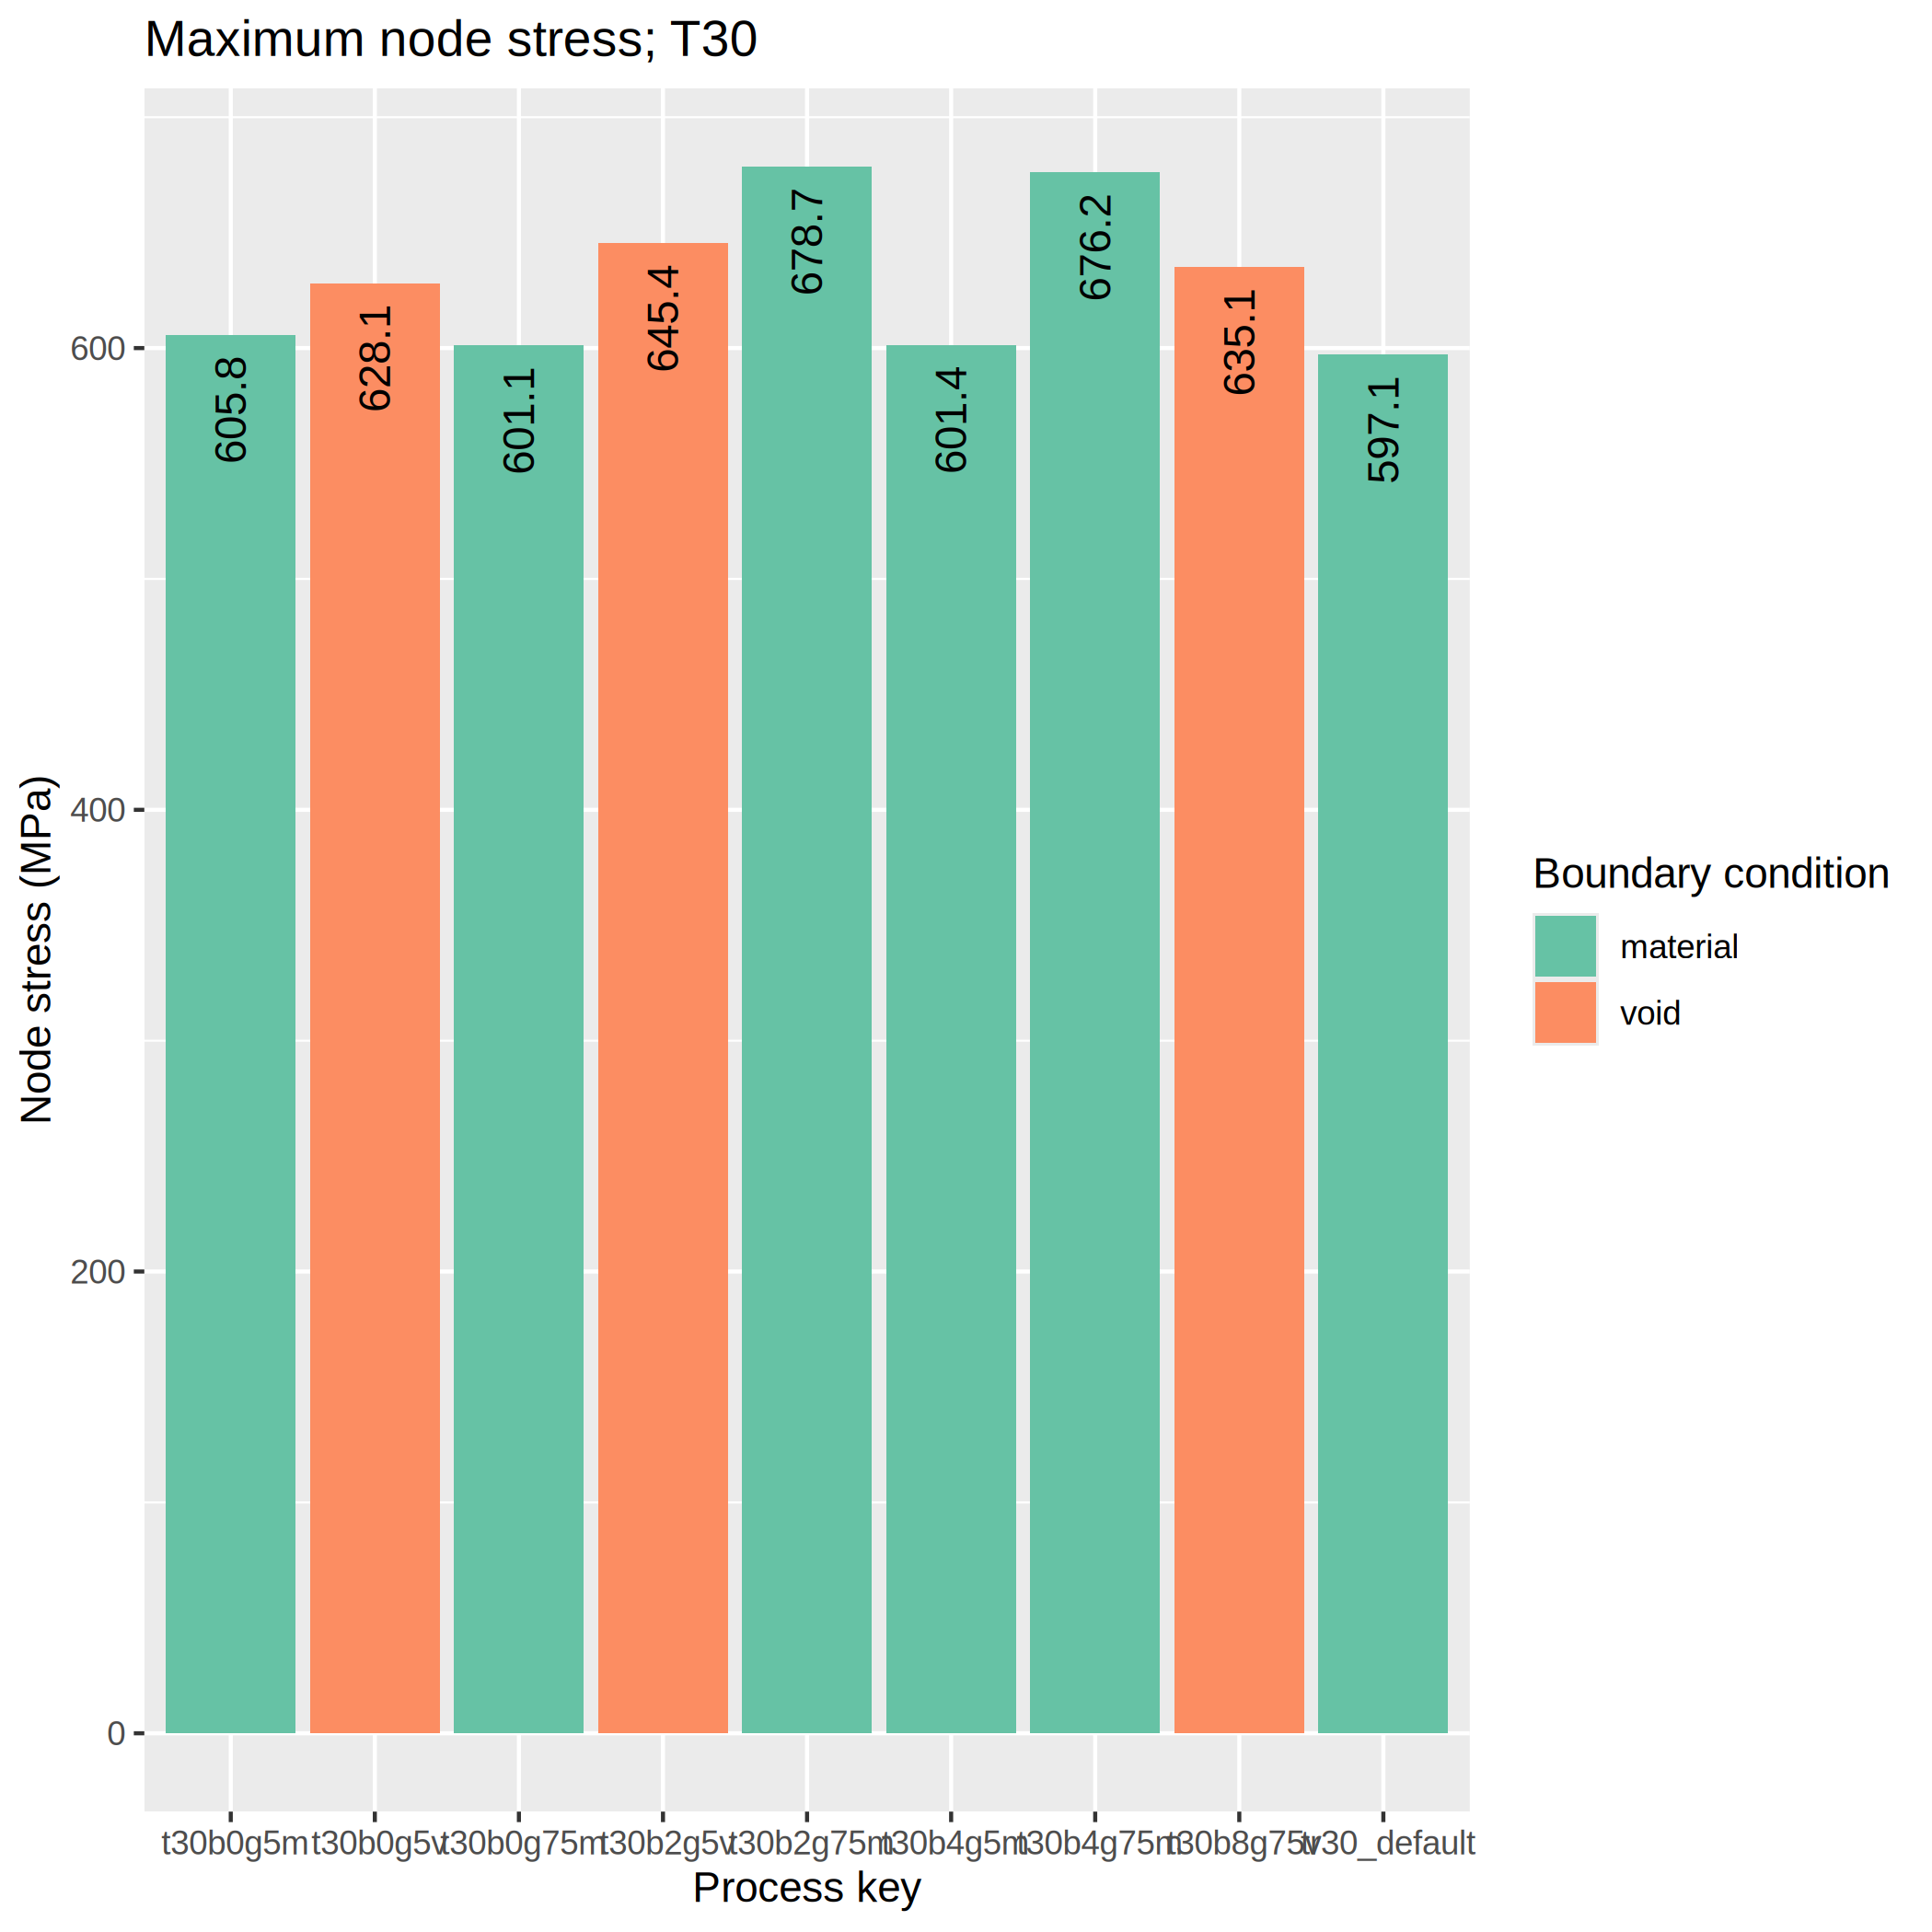
\includegraphics[width=\textwidth]{T30 _stressmax3.png}
    \label{}
  \end{subfigure}
  \caption{Results of 30\degree triangle.}
  \label{fig:tri30_results}
\end{figure}

\begin{figure}
  \centering 
  \begin{subfigure}[b]{0.45\textwidth}
    \centering 
    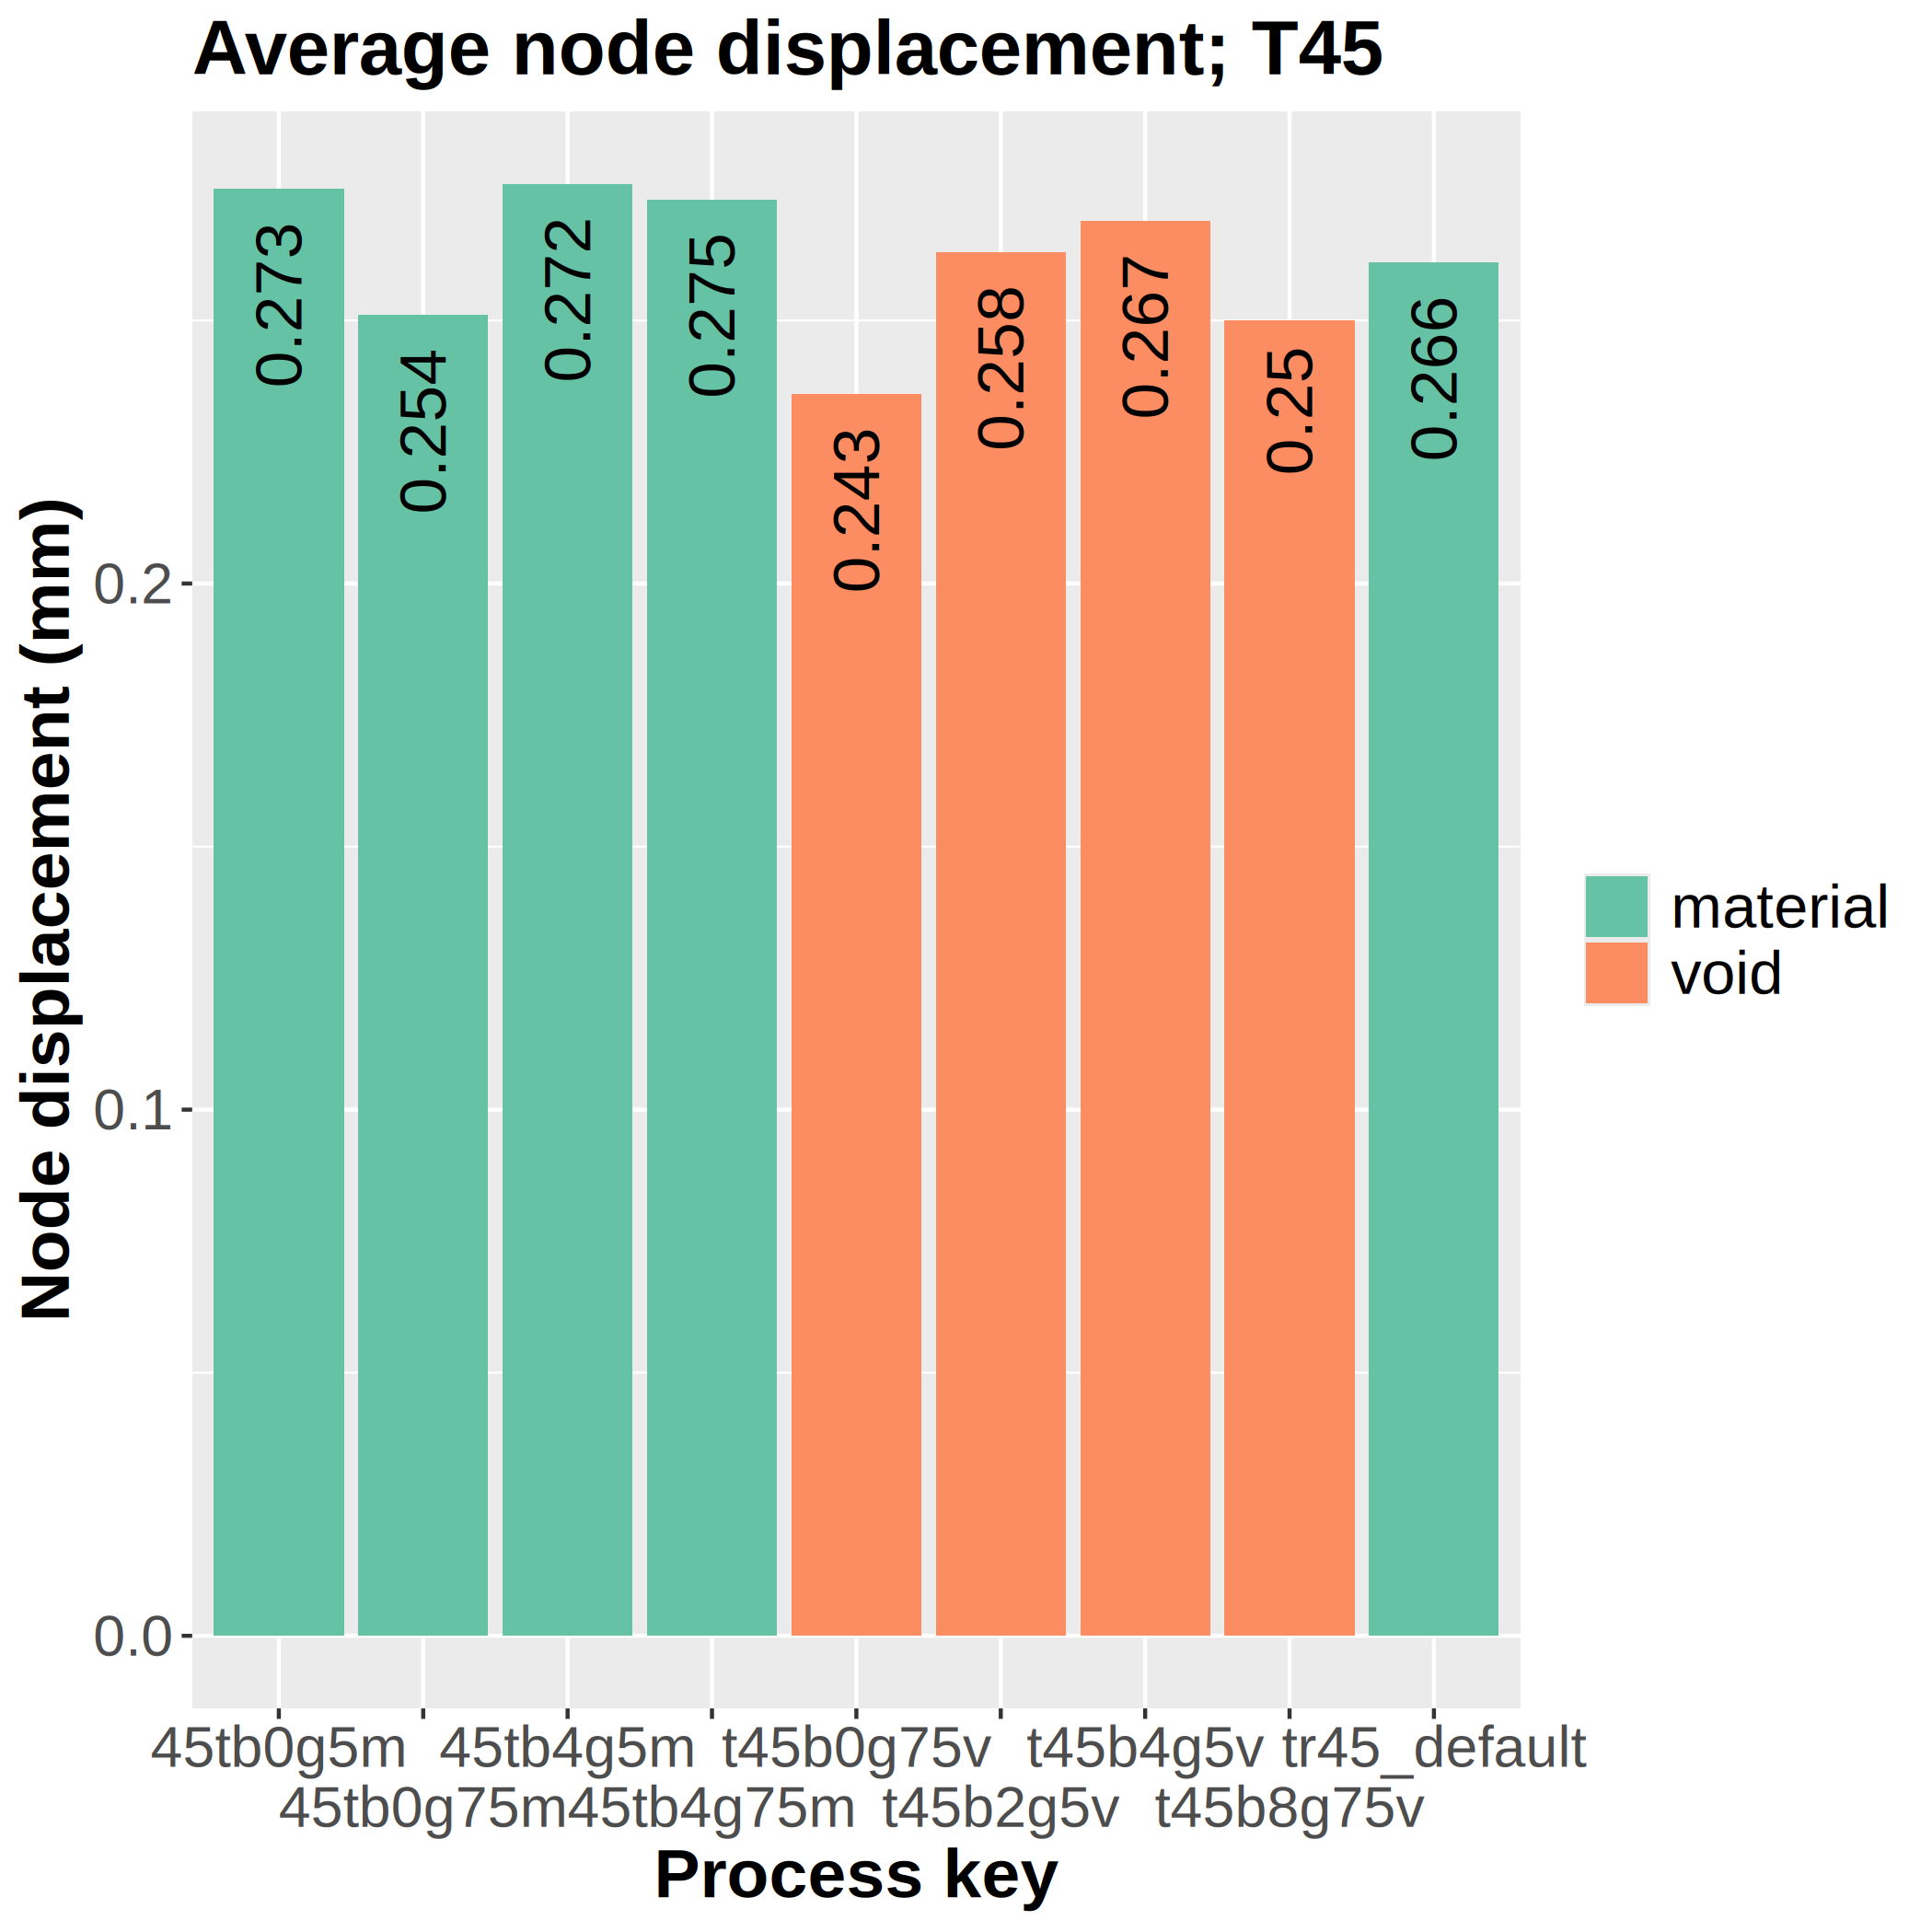
\includegraphics[width=\textwidth]{T45 _disp3.png}
    \label{}
  \end{subfigure}
  \begin{subfigure}[b]{0.45\textwidth}
    \centering 
    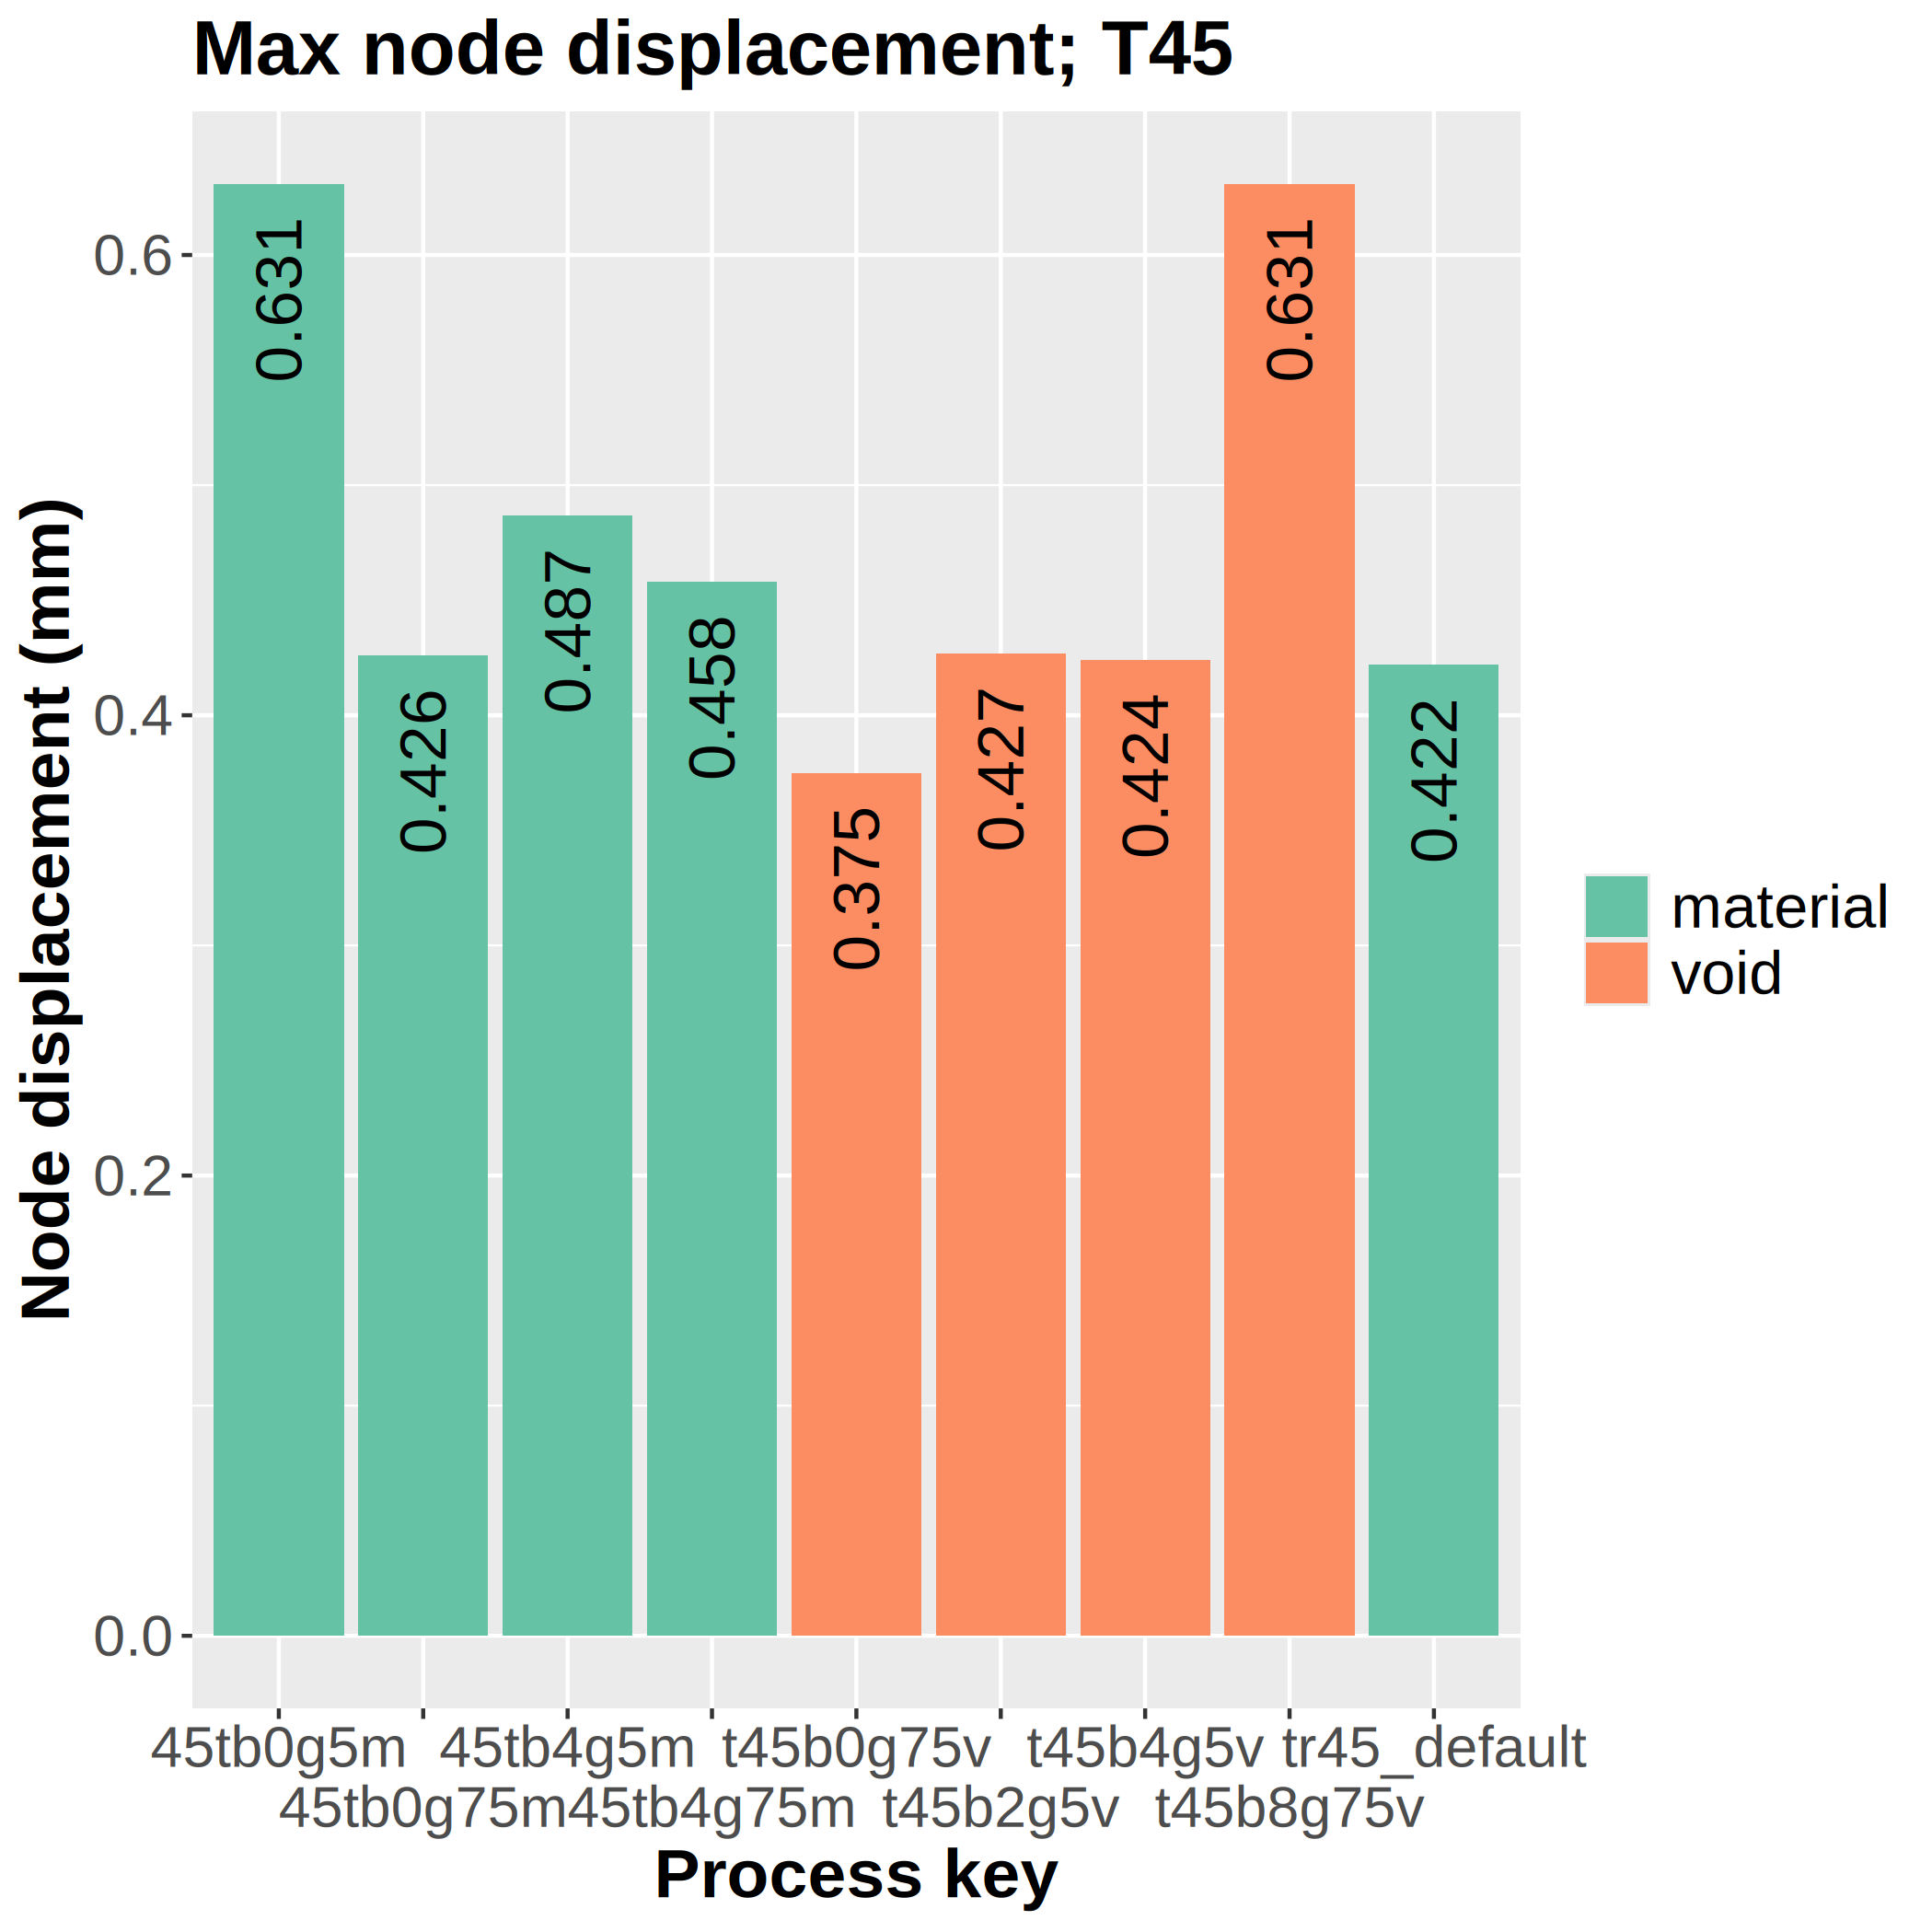
\includegraphics[width=\textwidth]{T45 _dispmax3.png}
    \label{}
  \end{subfigure}
  \begin{subfigure}[b]{0.45\textwidth}
    \centering 
    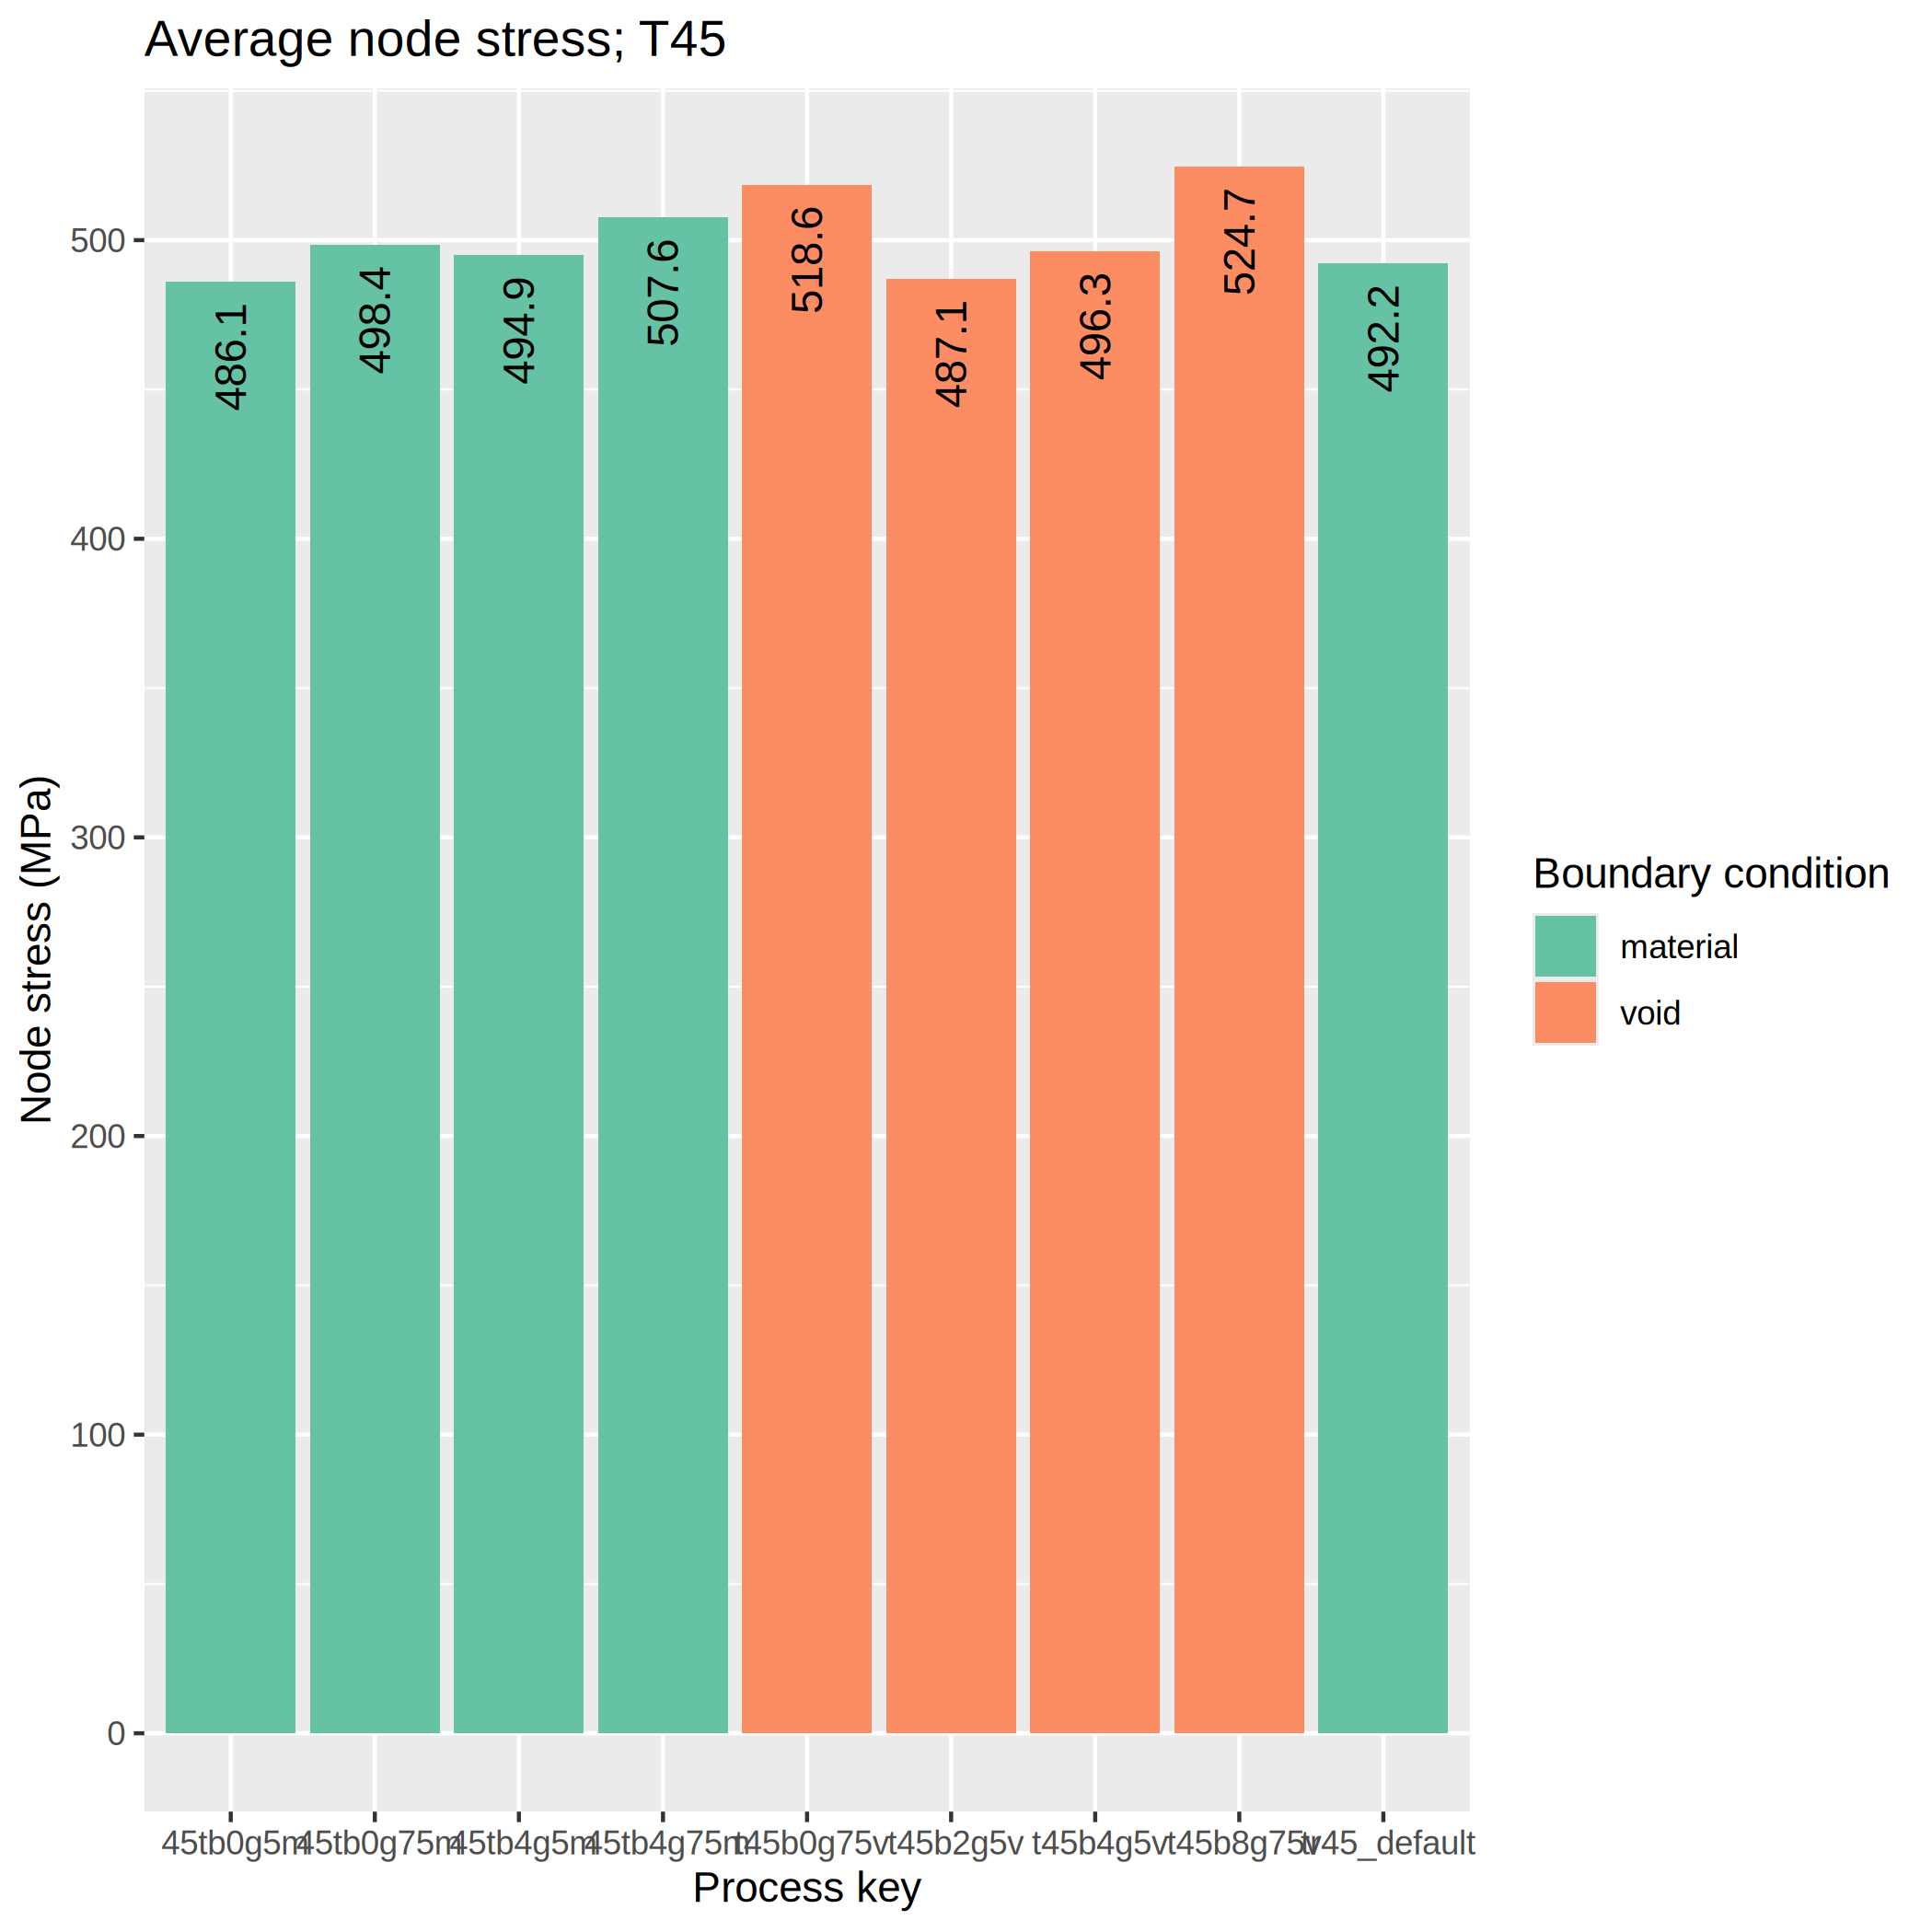
\includegraphics[width=\textwidth]{T45 _stress3.png}
    \label{}
  \end{subfigure}
  \begin{subfigure}[b]{0.45\textwidth}
    \centering 
    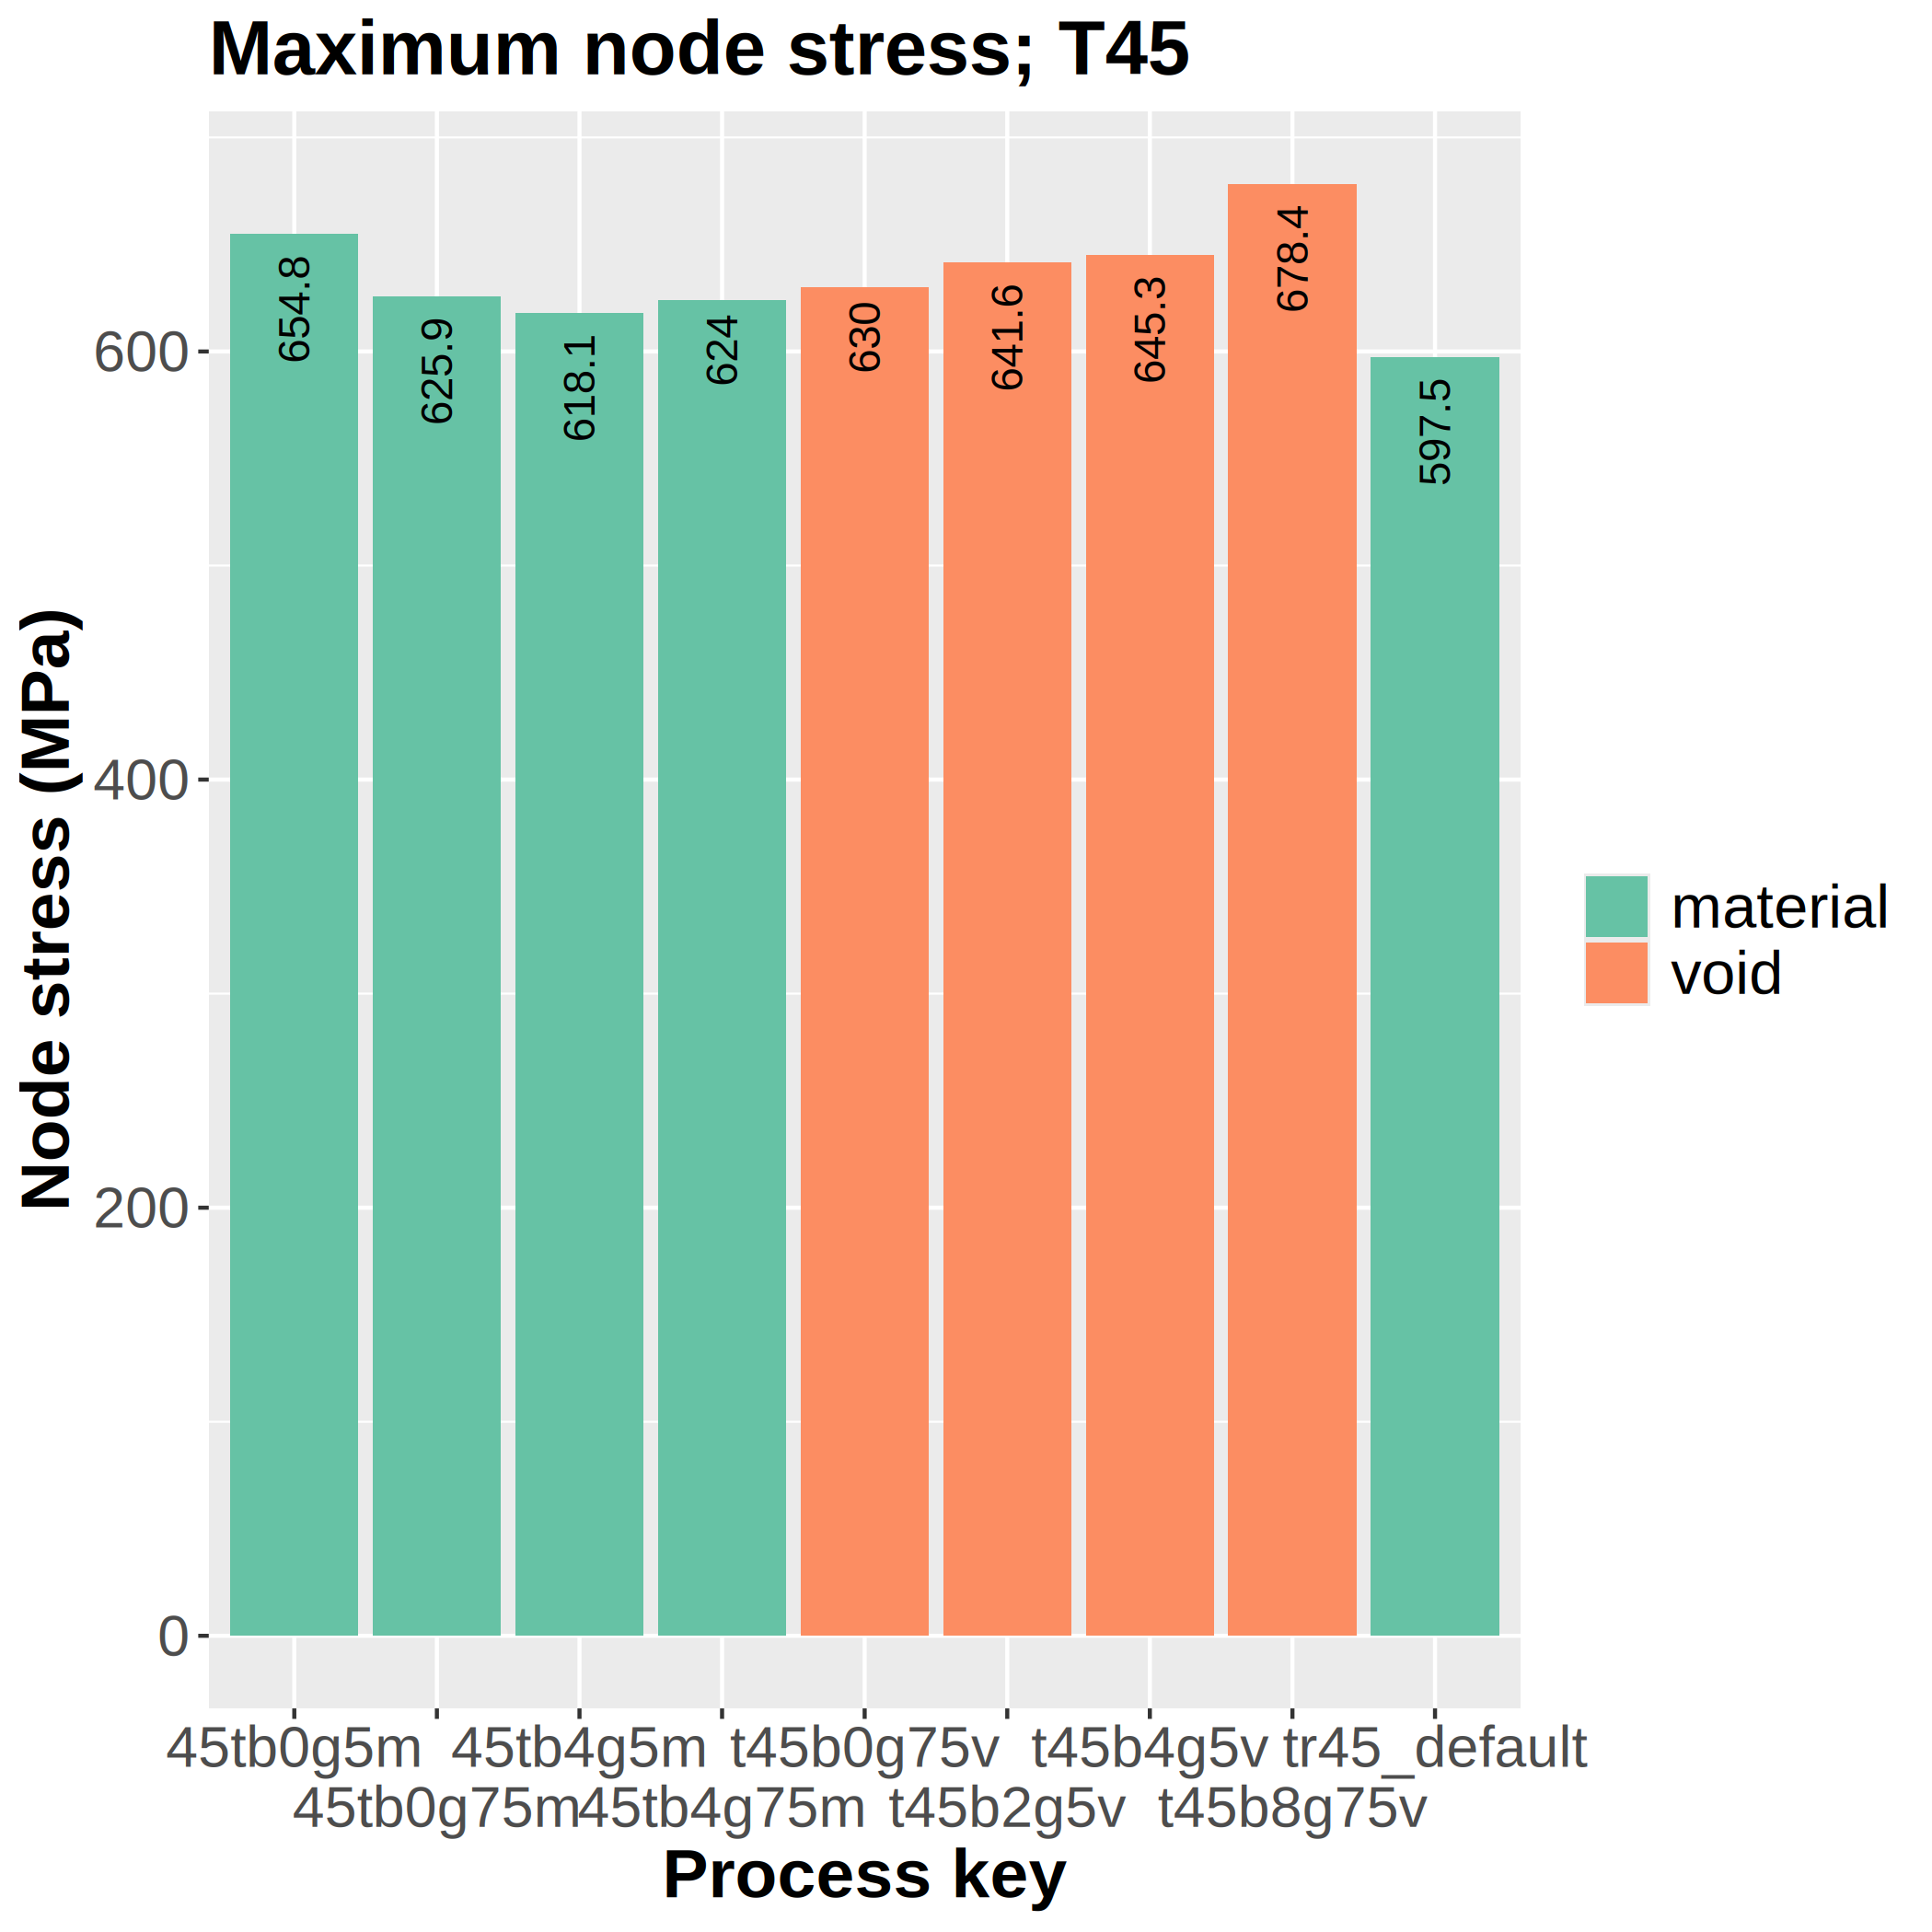
\includegraphics[width=\textwidth]{T45 _stressmax3.png}
    \label{}
  \end{subfigure}
  \caption{Results of 45\degree triangle.}
  \label{fig:tri45_results}
\end{figure}

\begin{figure}[h!]
  \centering 
  \begin{subfigure}[b]{0.45\textwidth}
    \centering 
    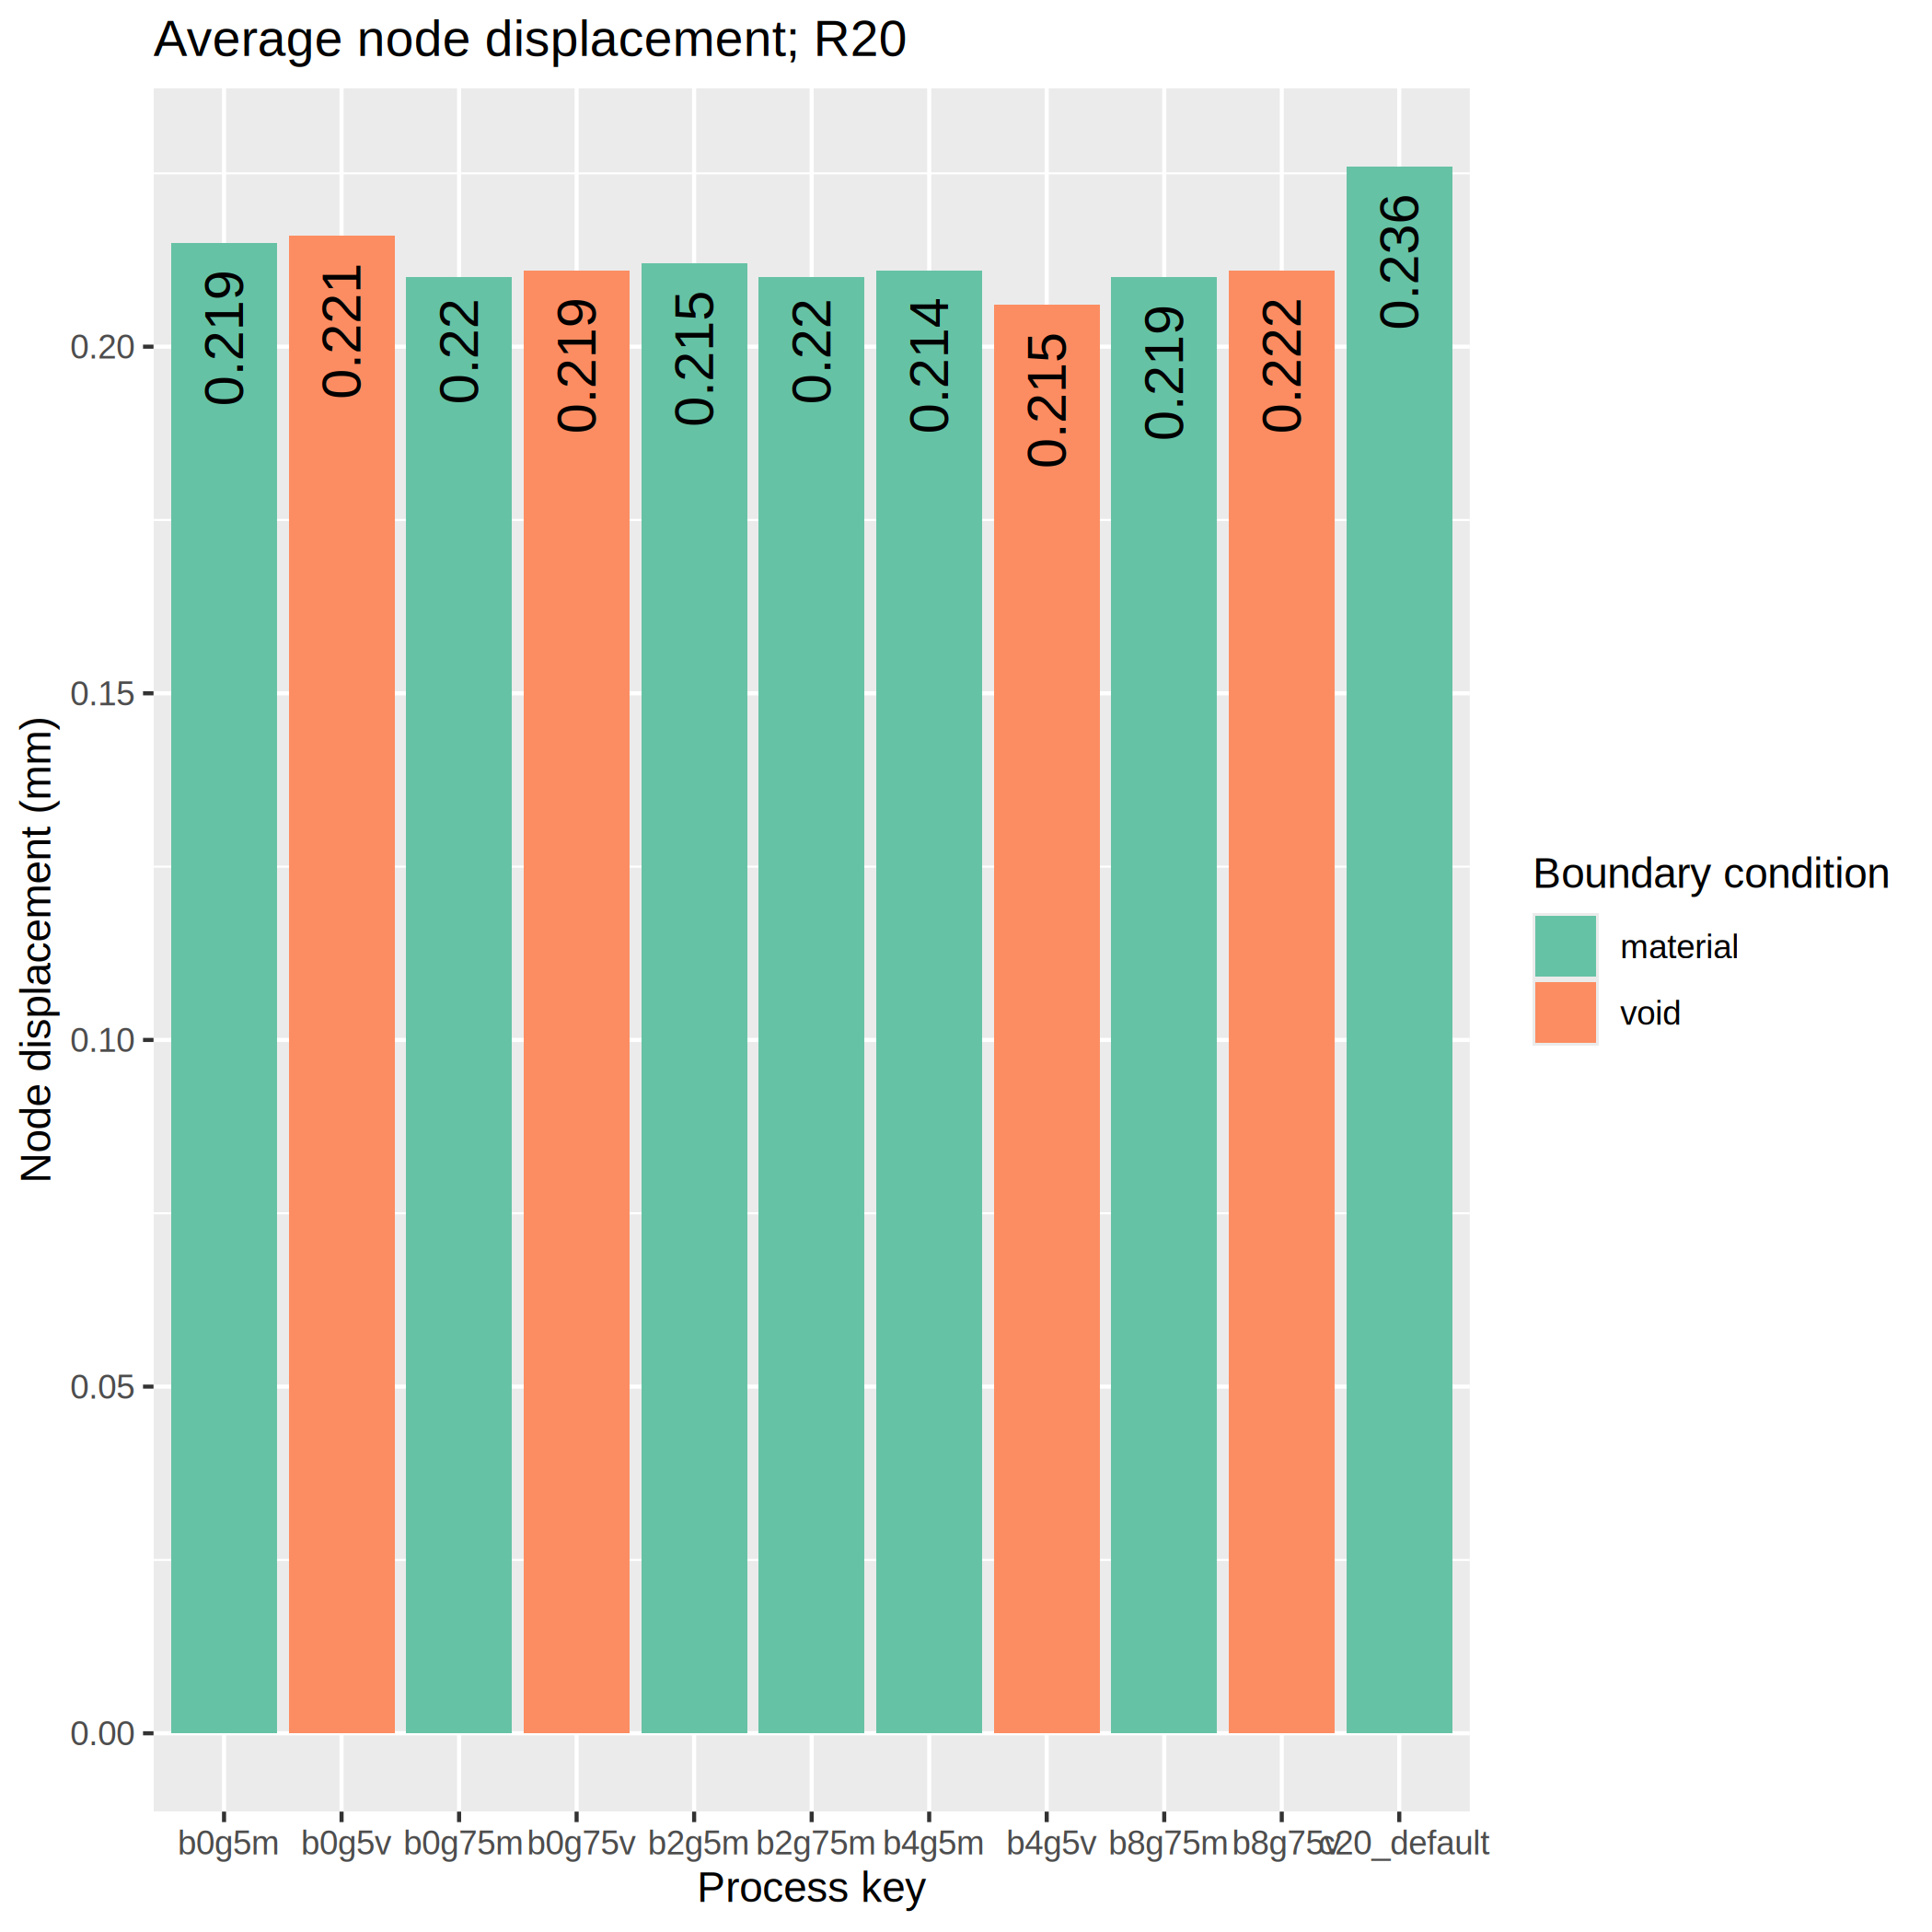
\includegraphics[width=\textwidth]{R20 _disp3.png}
    \label{}
  \end{subfigure}
  \begin{subfigure}[b]{0.45\textwidth}
    \centering 
    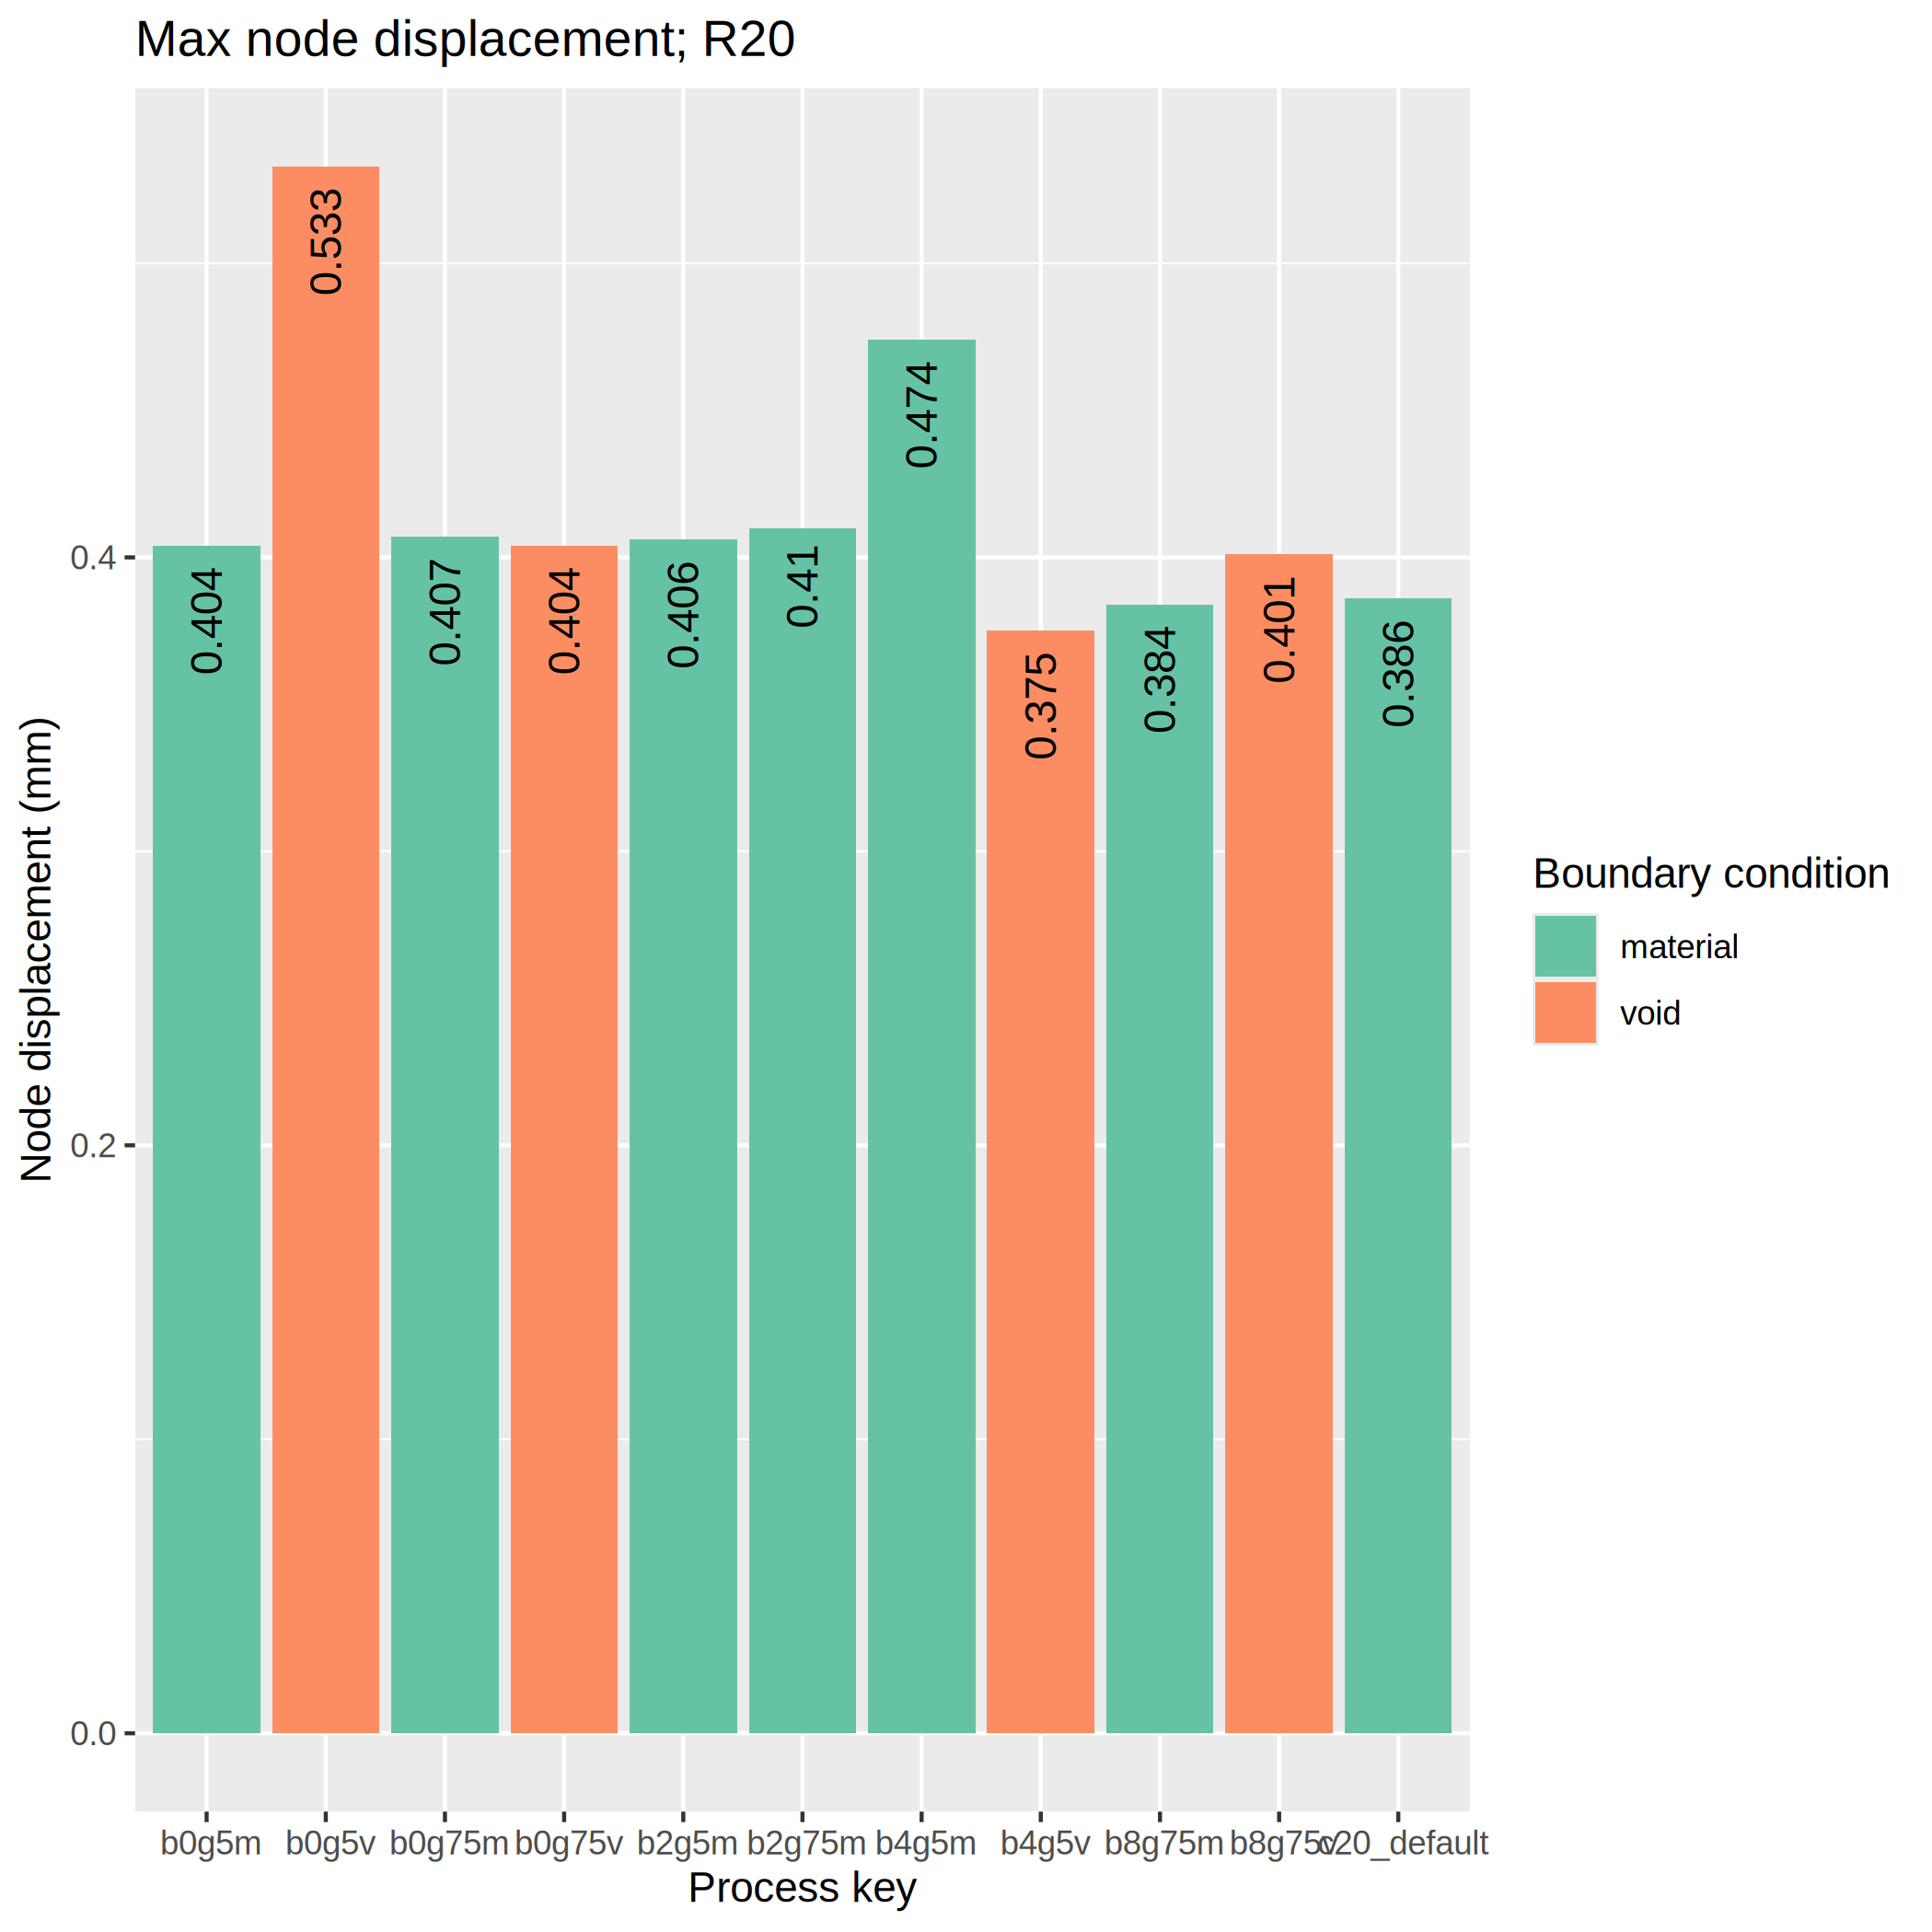
\includegraphics[width=\textwidth]{R20 _dispmax3.png}
    \label{}
  \end{subfigure}
  \begin{subfigure}[b]{0.45\textwidth}
    \centering 
    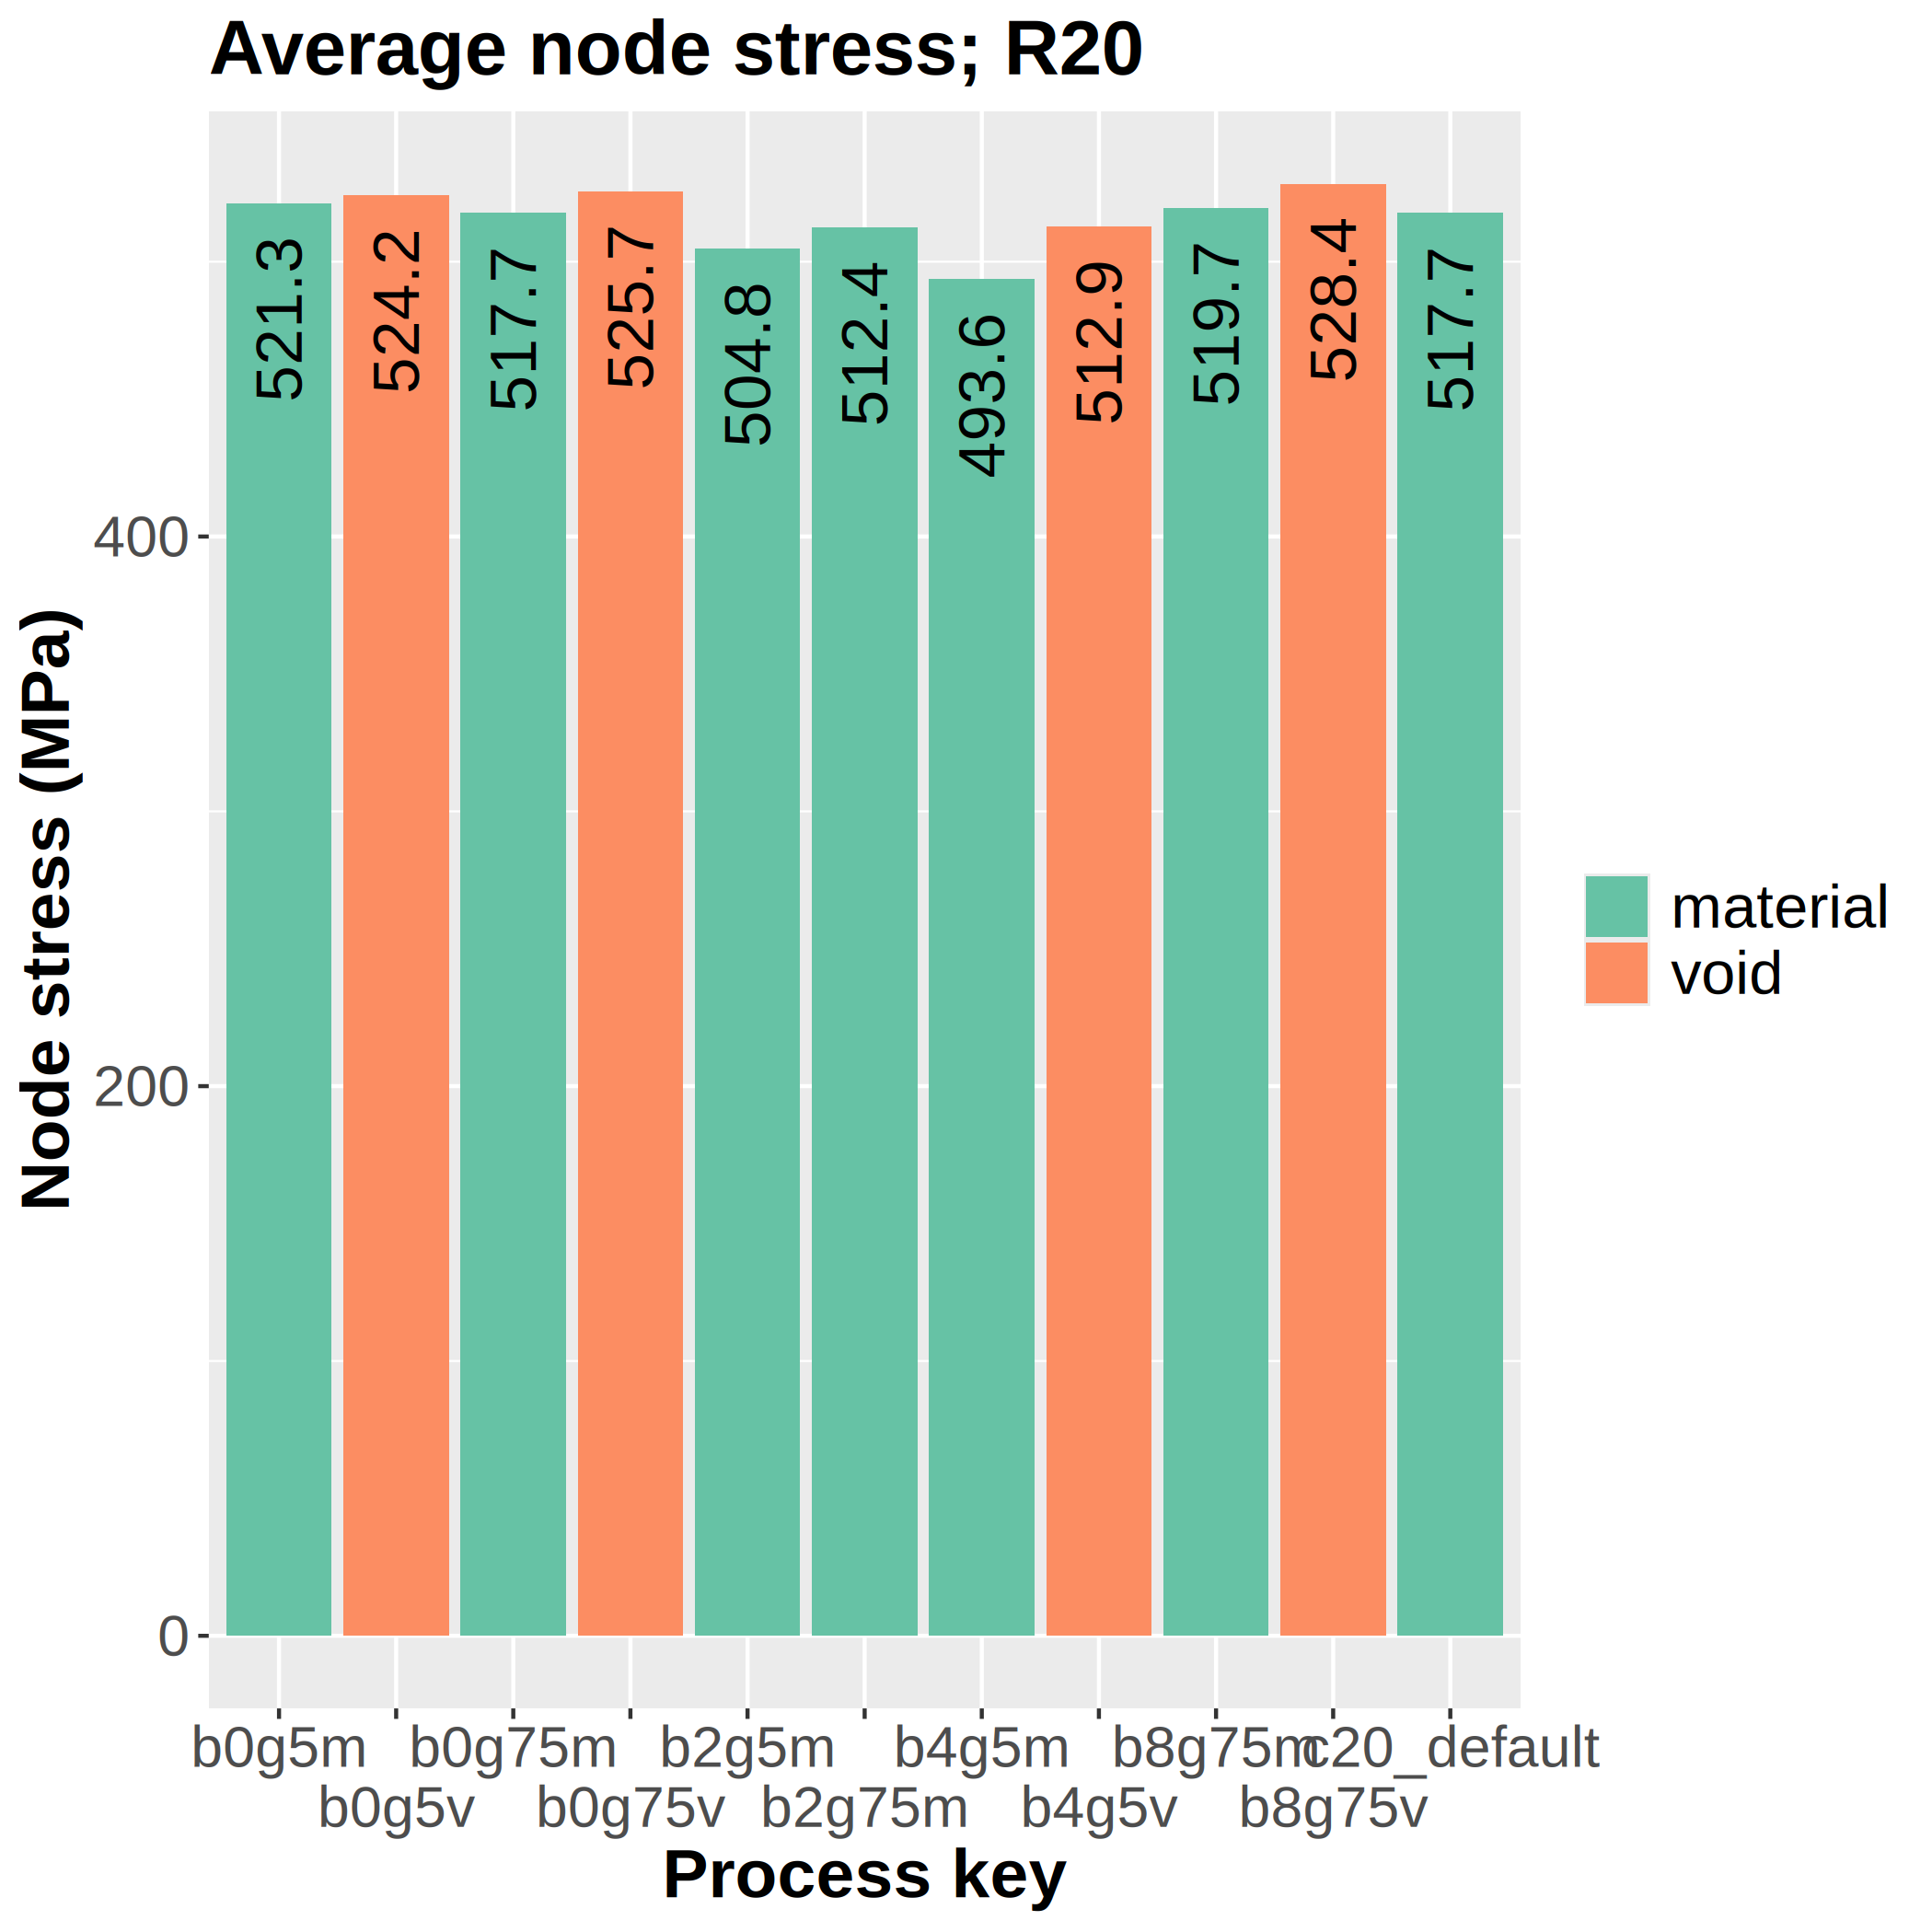
\includegraphics[width=\textwidth]{R20 _stress3.png}
    \label{}
  \end{subfigure}
  \begin{subfigure}[b]{0.45\textwidth}
    \centering 
    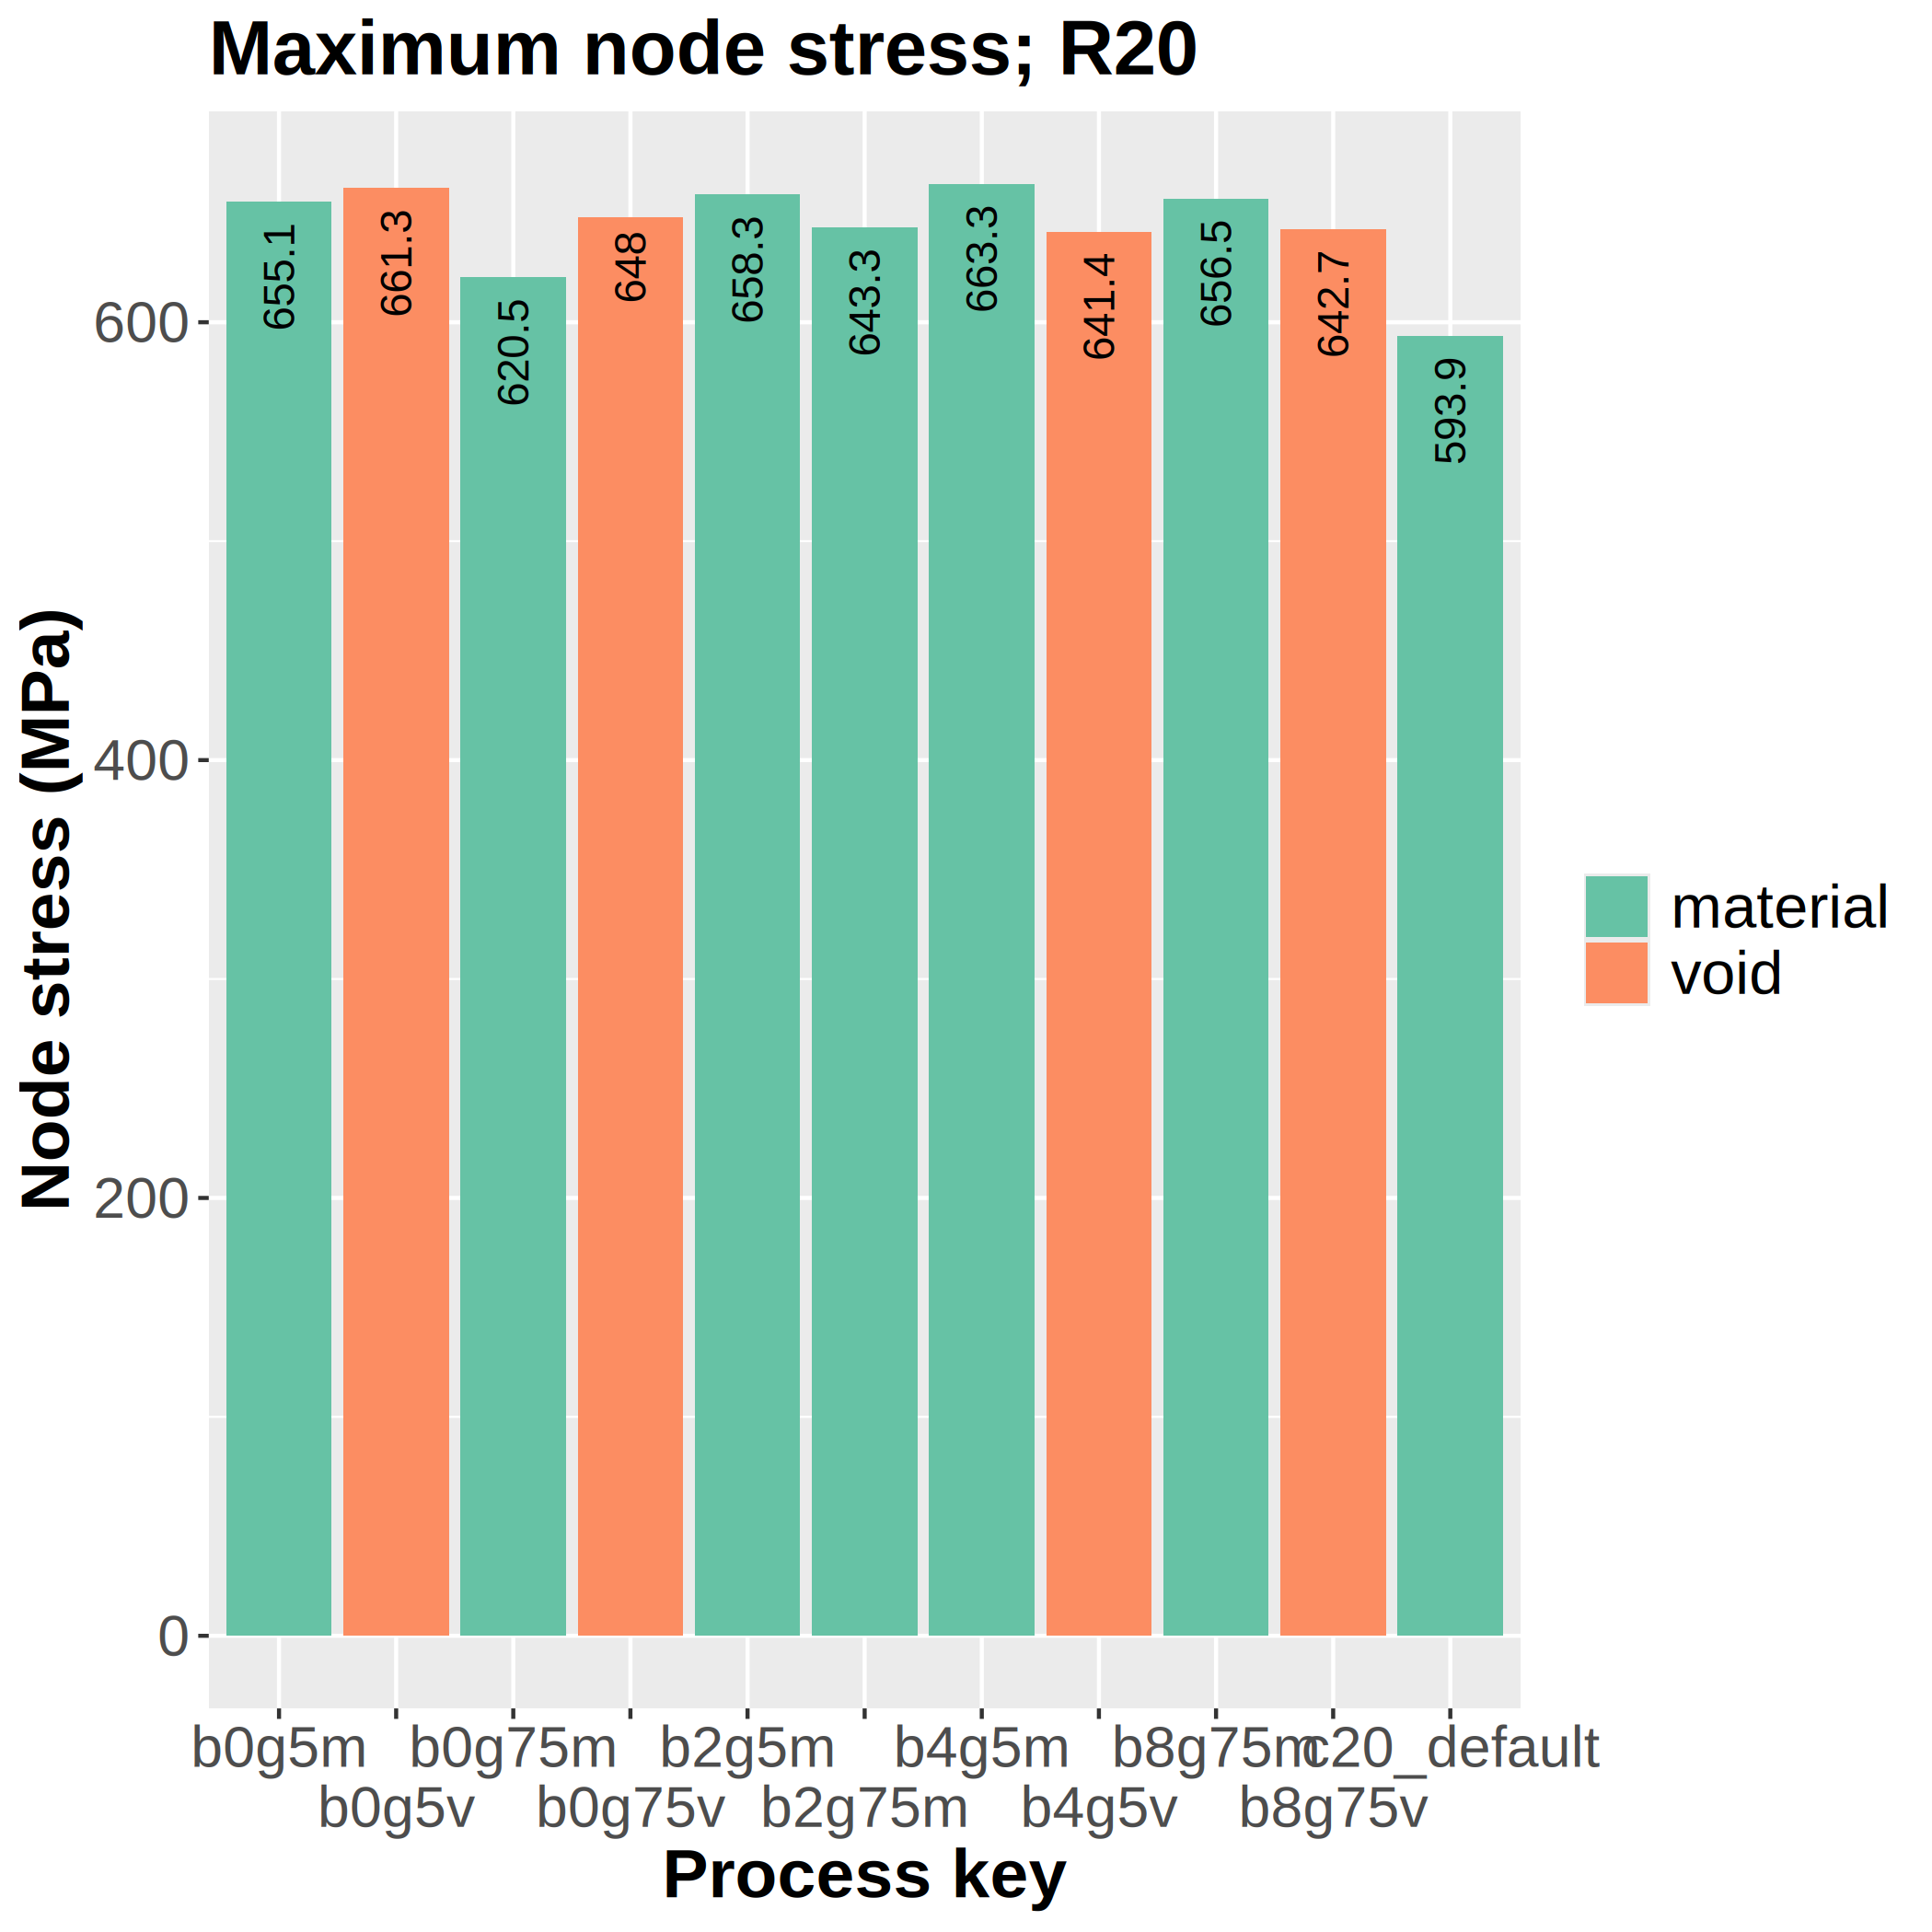
\includegraphics[width=\textwidth]{R20 _stressmax3.png}
    \label{}
  \end{subfigure}
  \caption{Results of 20R fillet.}
  \label{fig:20r_results}
\end{figure}

\begin{figure}
  \centering 
  \begin{subfigure}[b]{0.45\textwidth}
    \centering 
    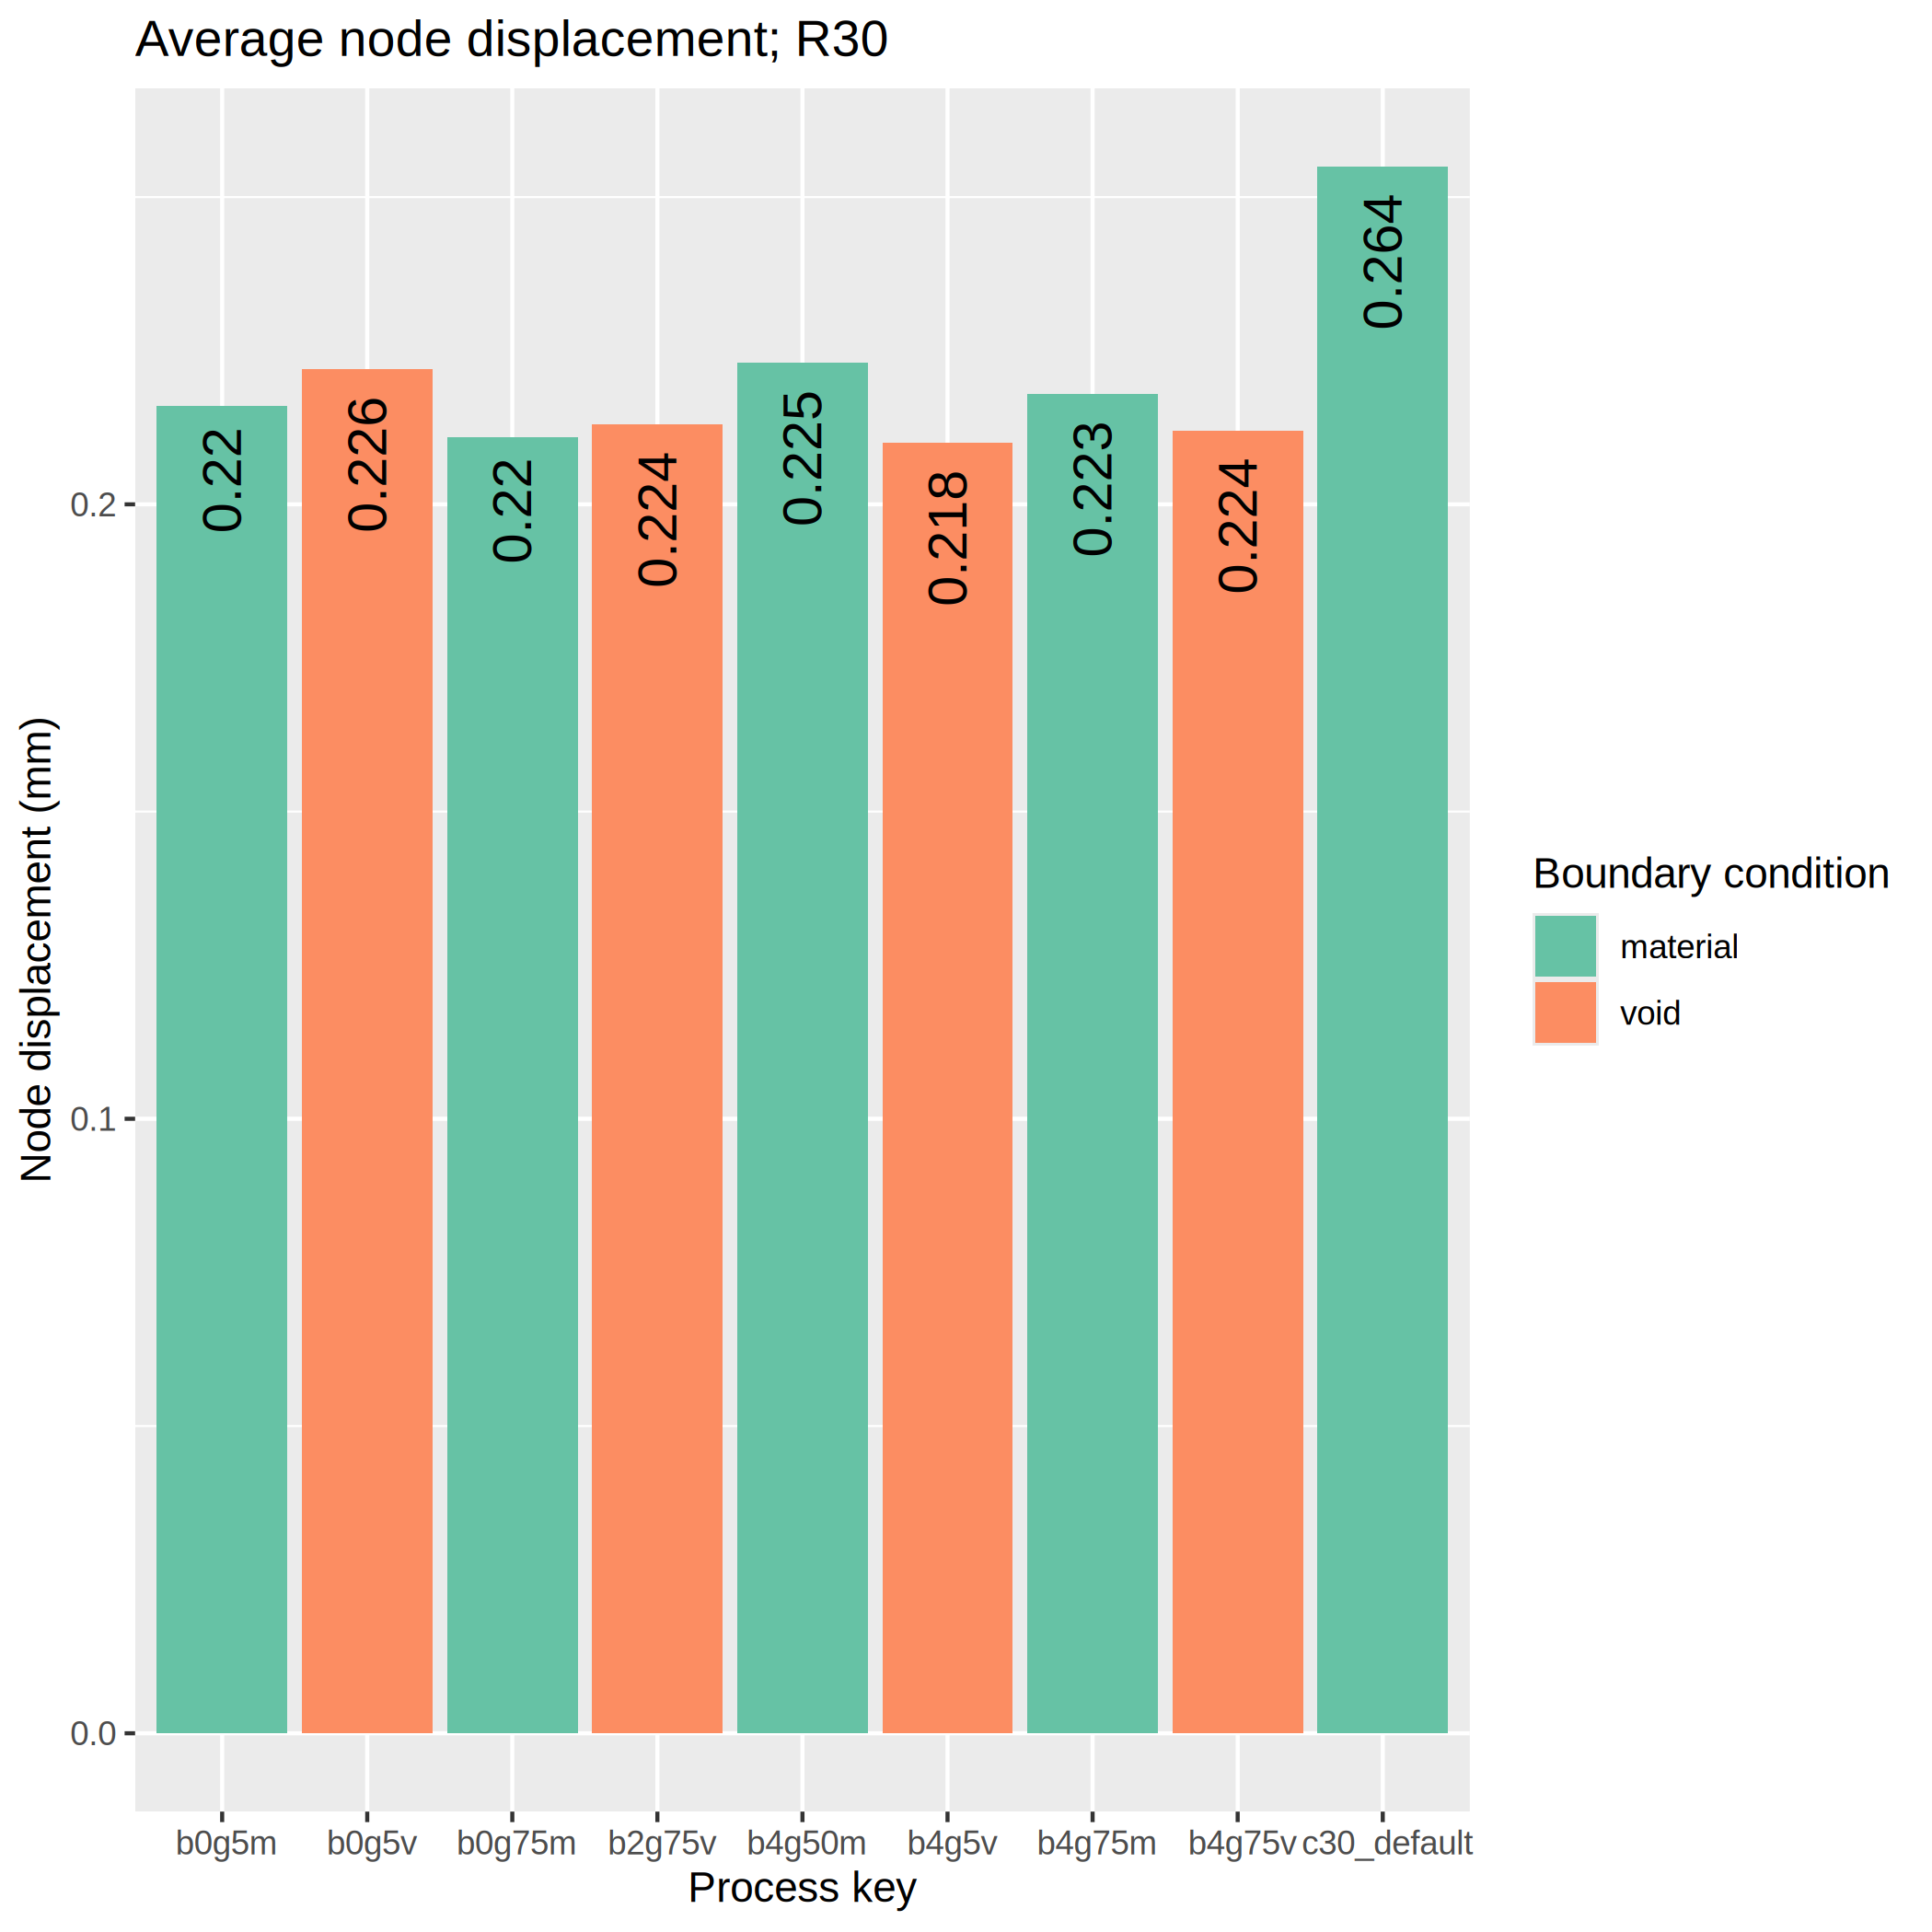
\includegraphics[width=\textwidth]{R30 _disp3.png}
    \label{}
  \end{subfigure}
  \begin{subfigure}[b]{0.45\textwidth}
    \centering 
    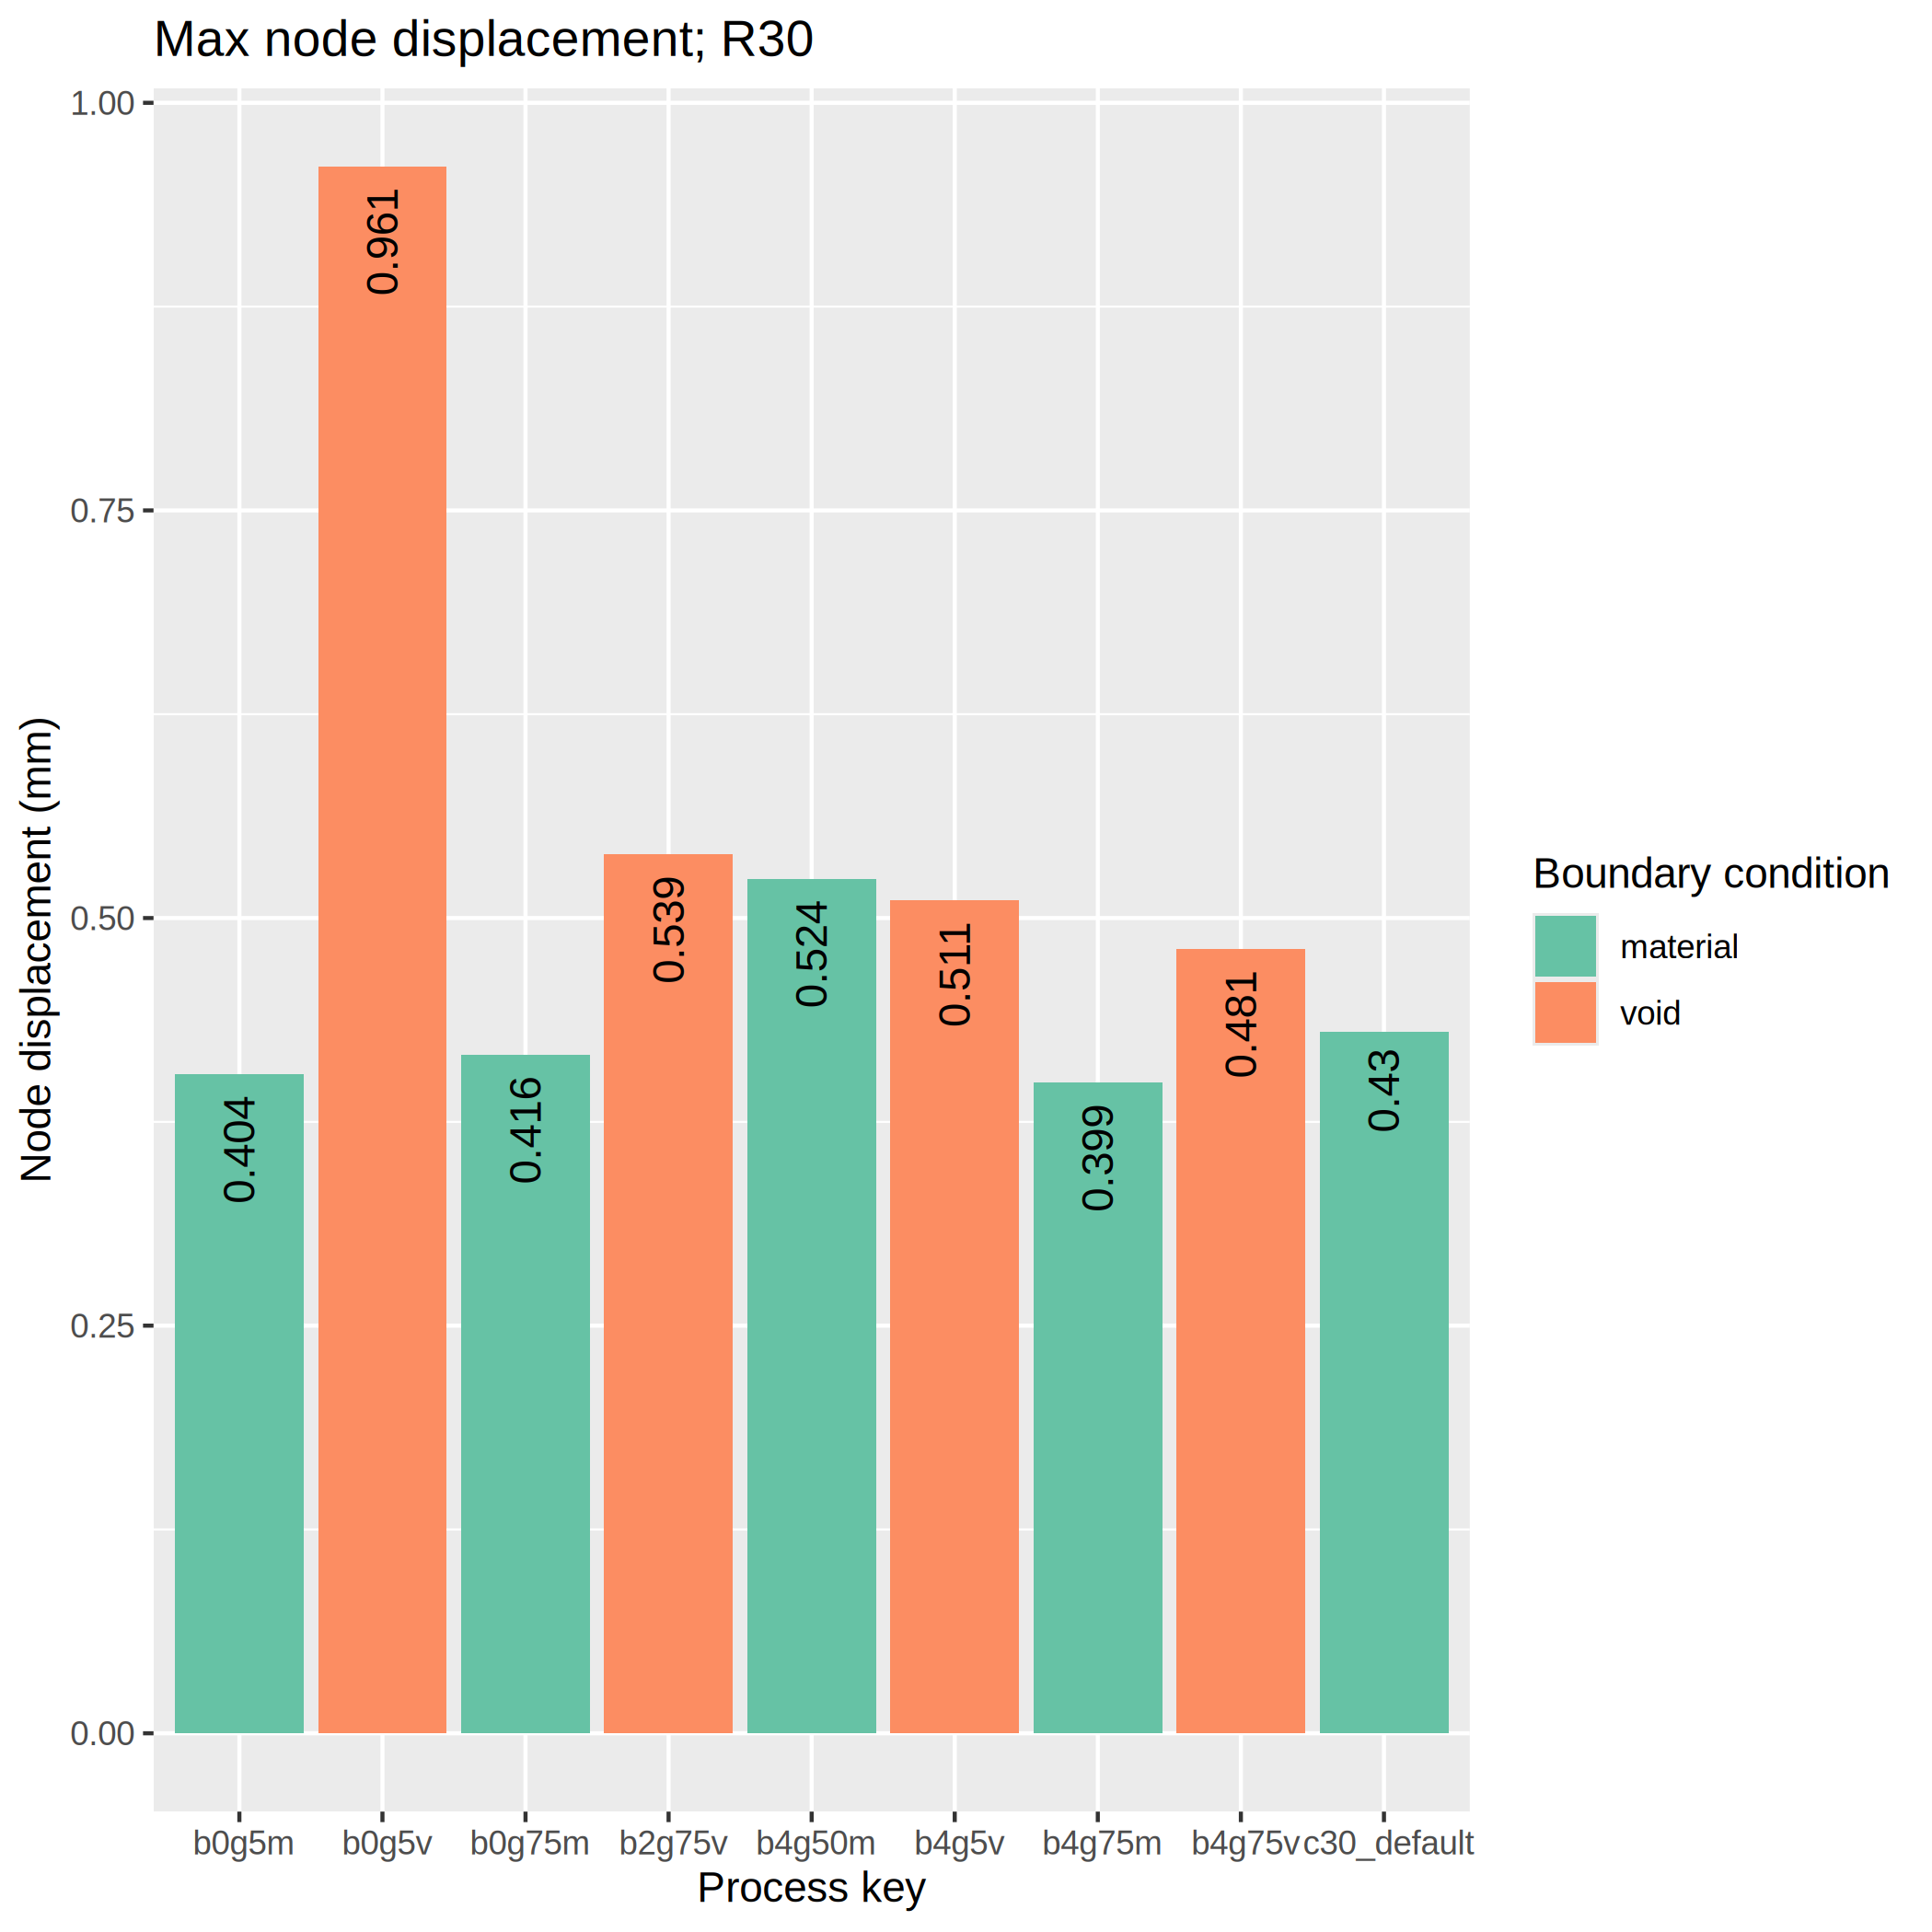
\includegraphics[width=\textwidth]{R30 _dispmax3.png}
    \label{}
  \end{subfigure}
  \begin{subfigure}[b]{0.45\textwidth}
    \centering 
    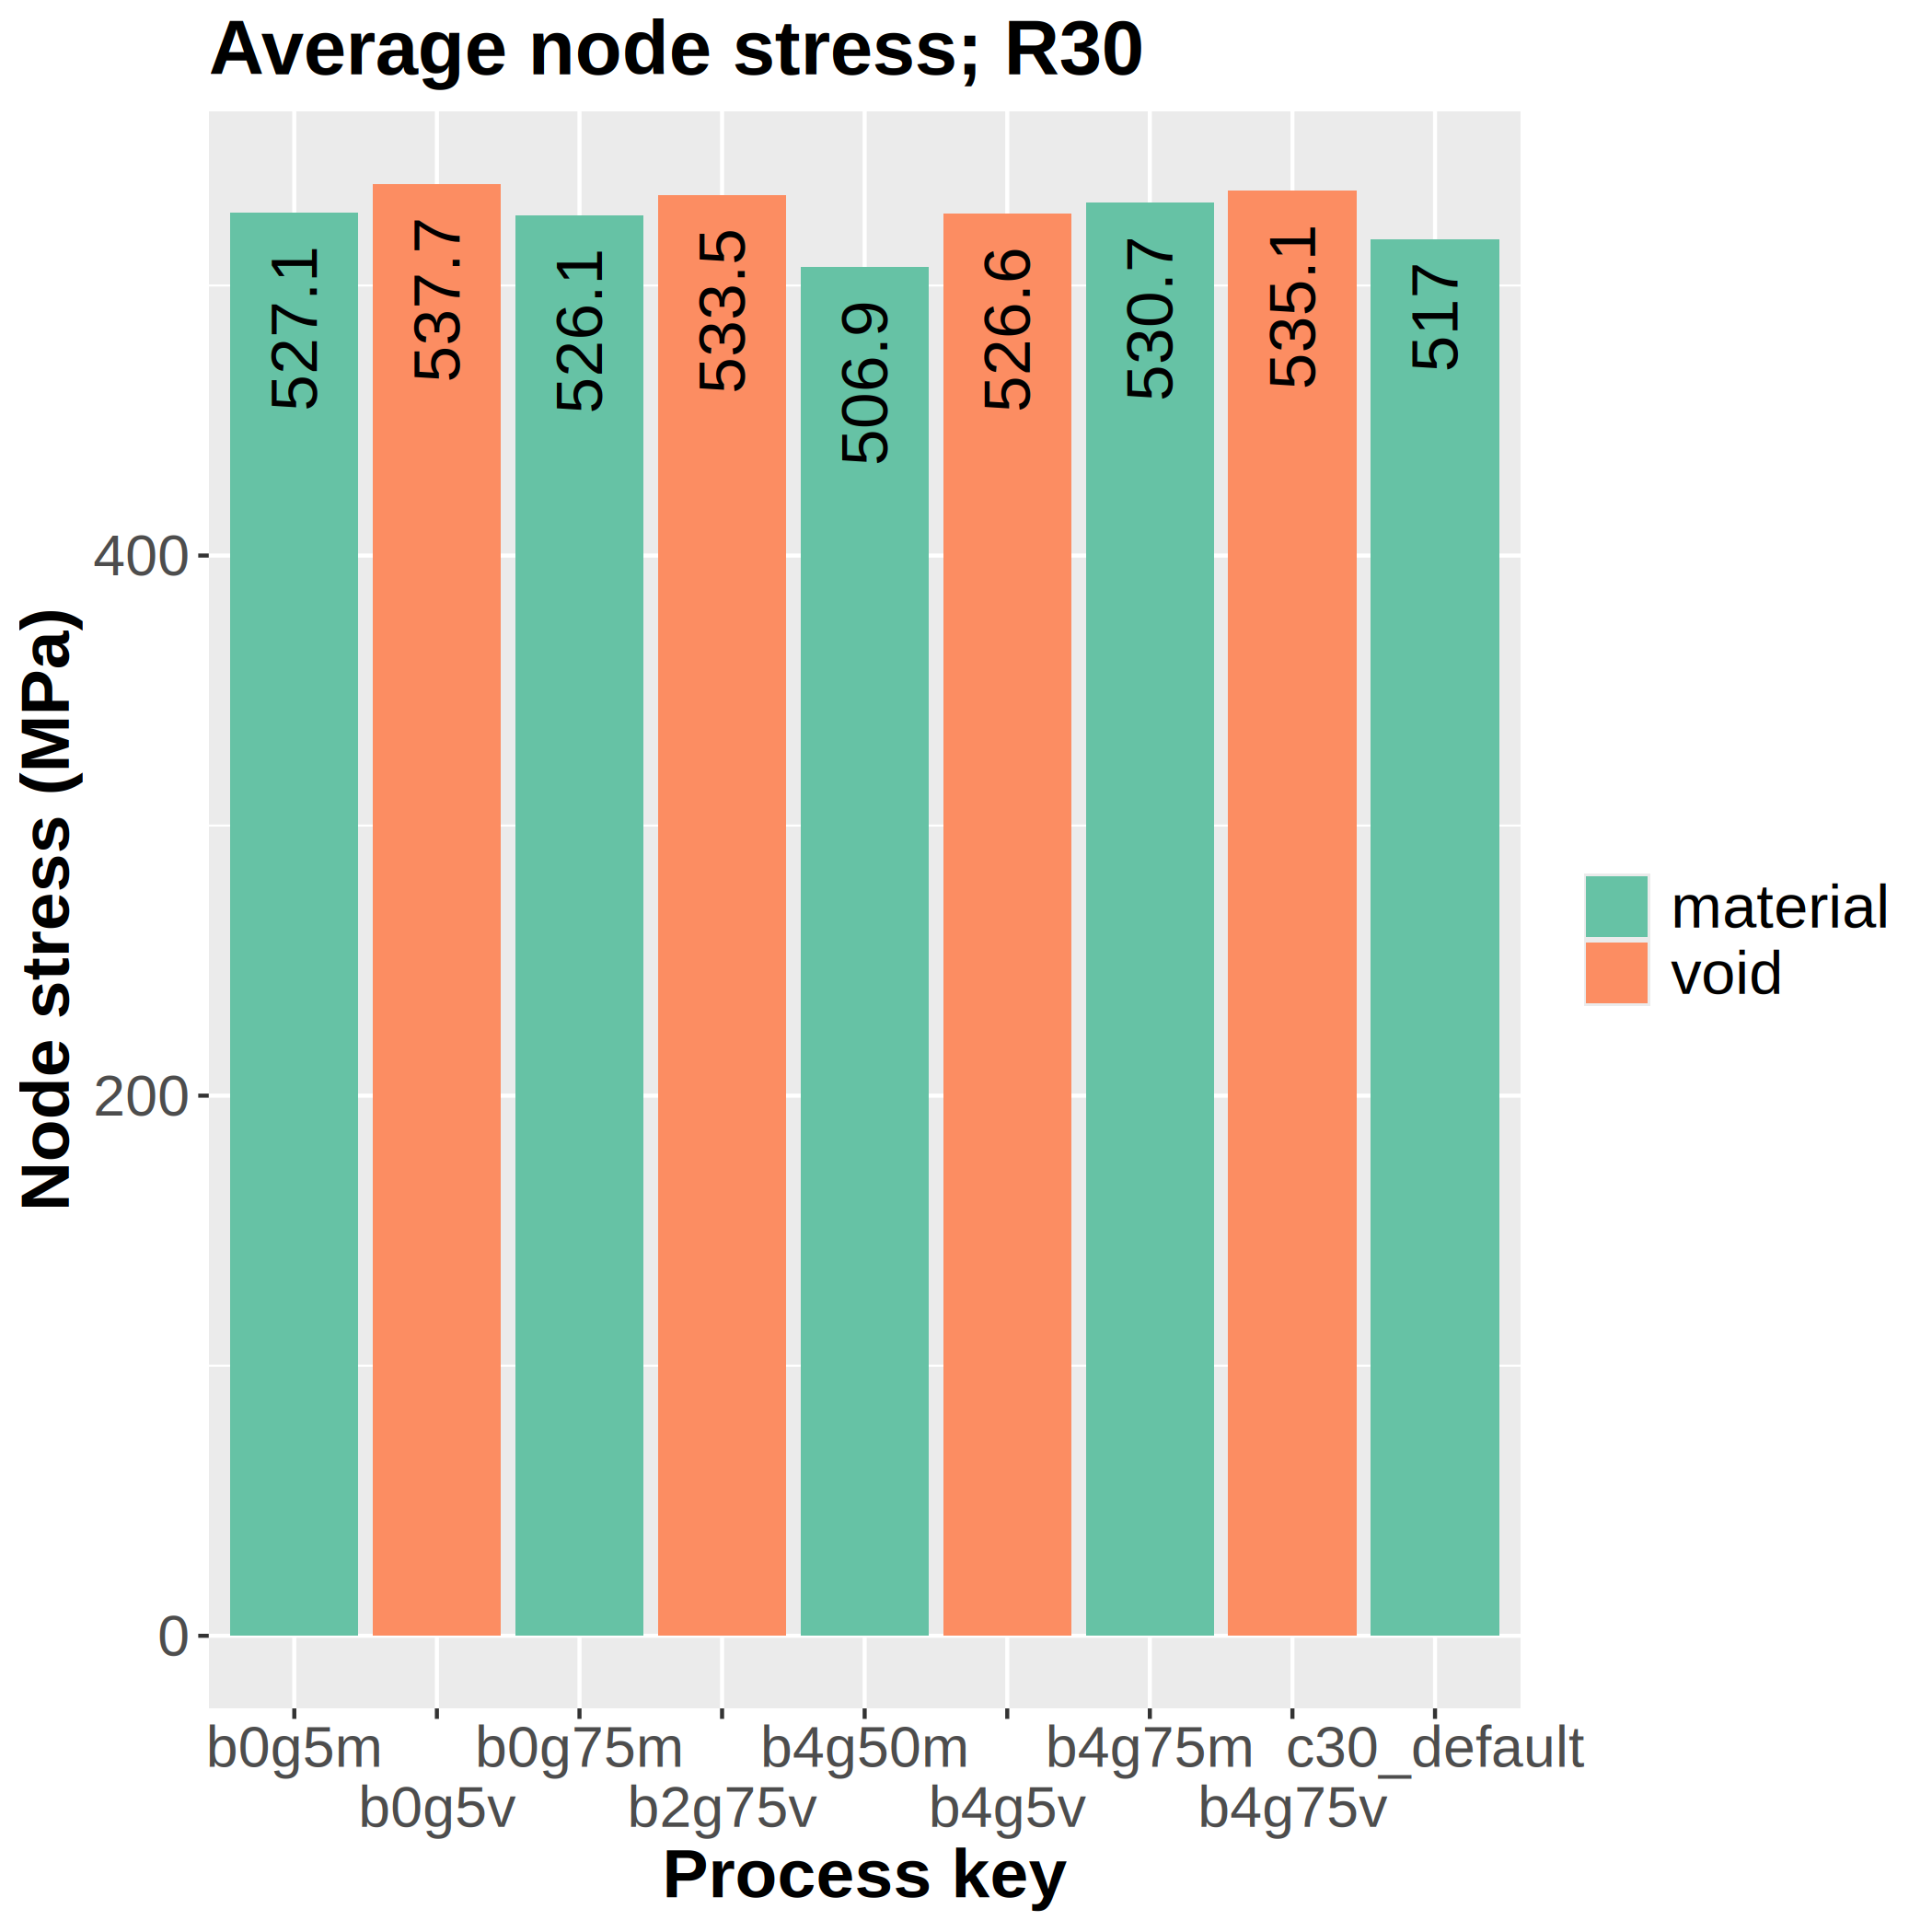
\includegraphics[width=\textwidth]{R30 _stress3.png}
    \label{}
  \end{subfigure}
  \begin{subfigure}[b]{0.45\textwidth}
    \centering 
    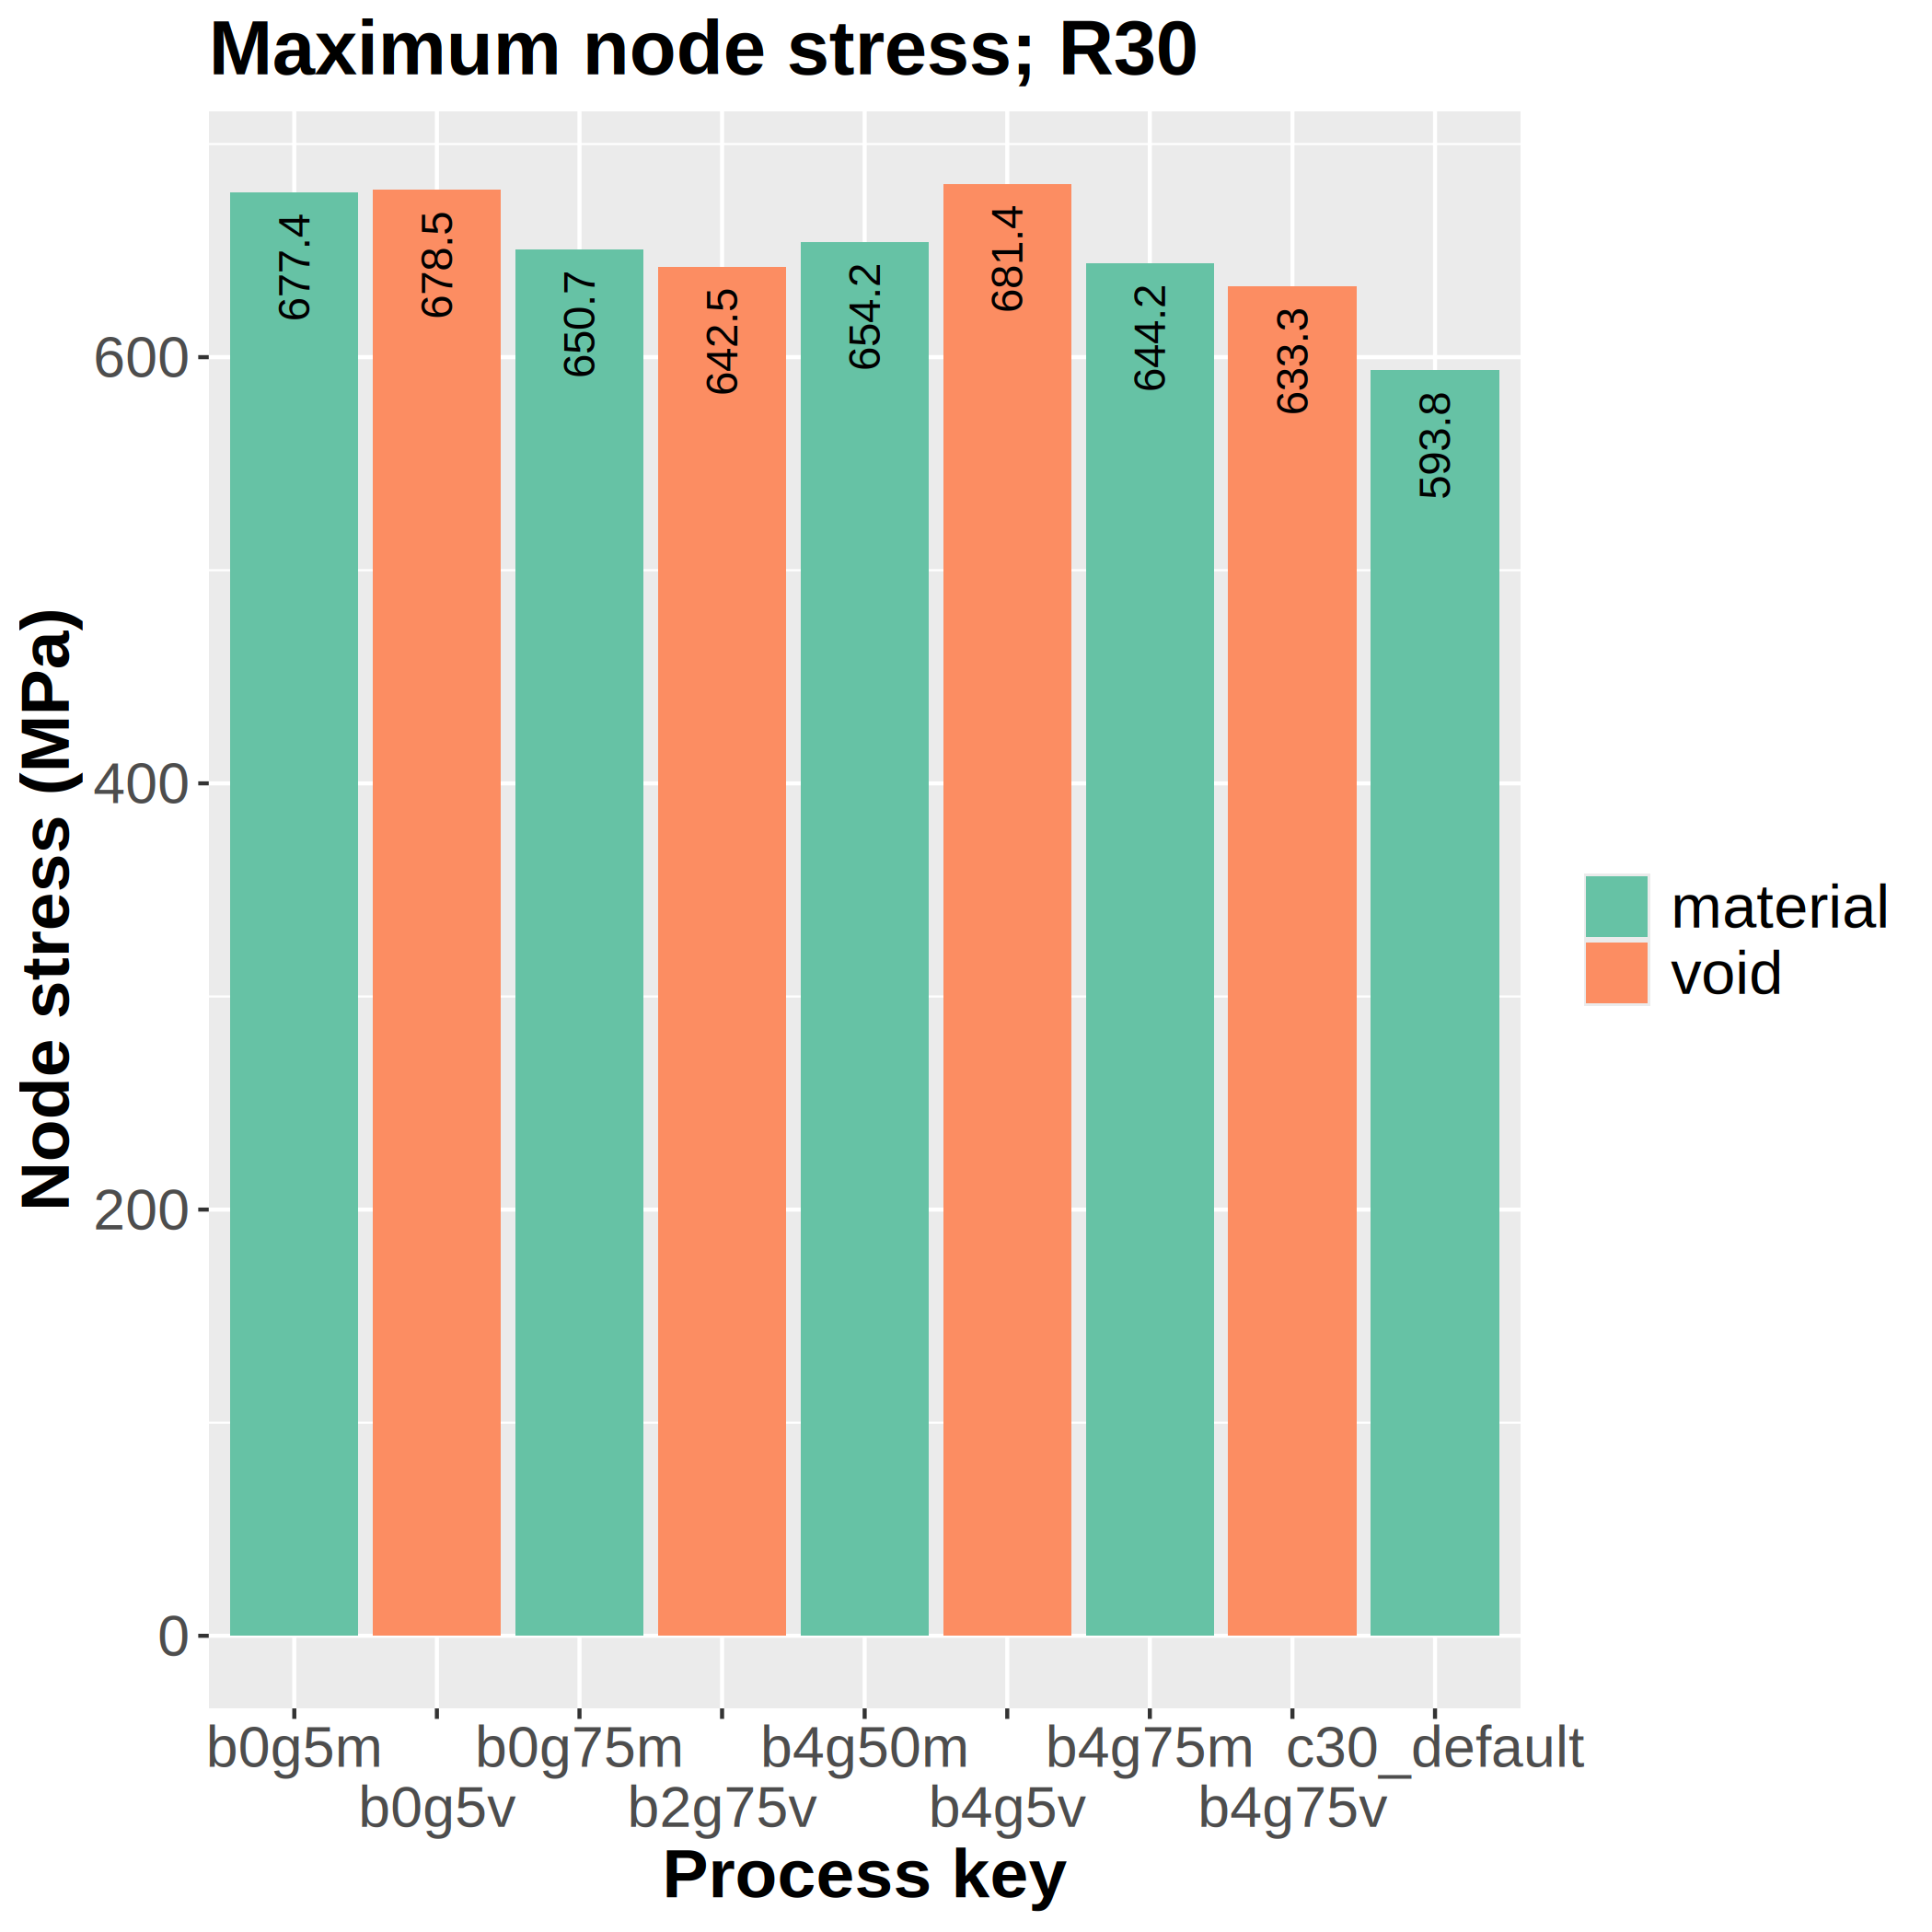
\includegraphics[width=\textwidth]{R30 _stressmax3.png}
    \label{}
  \end{subfigure}
  \caption{Results of 30R fillet.}
  \label{fig:30r_results}
\end{figure}

\begin{figure}
  \centering 
  \begin{subfigure}[b]{0.45\textwidth}
    \centering 
    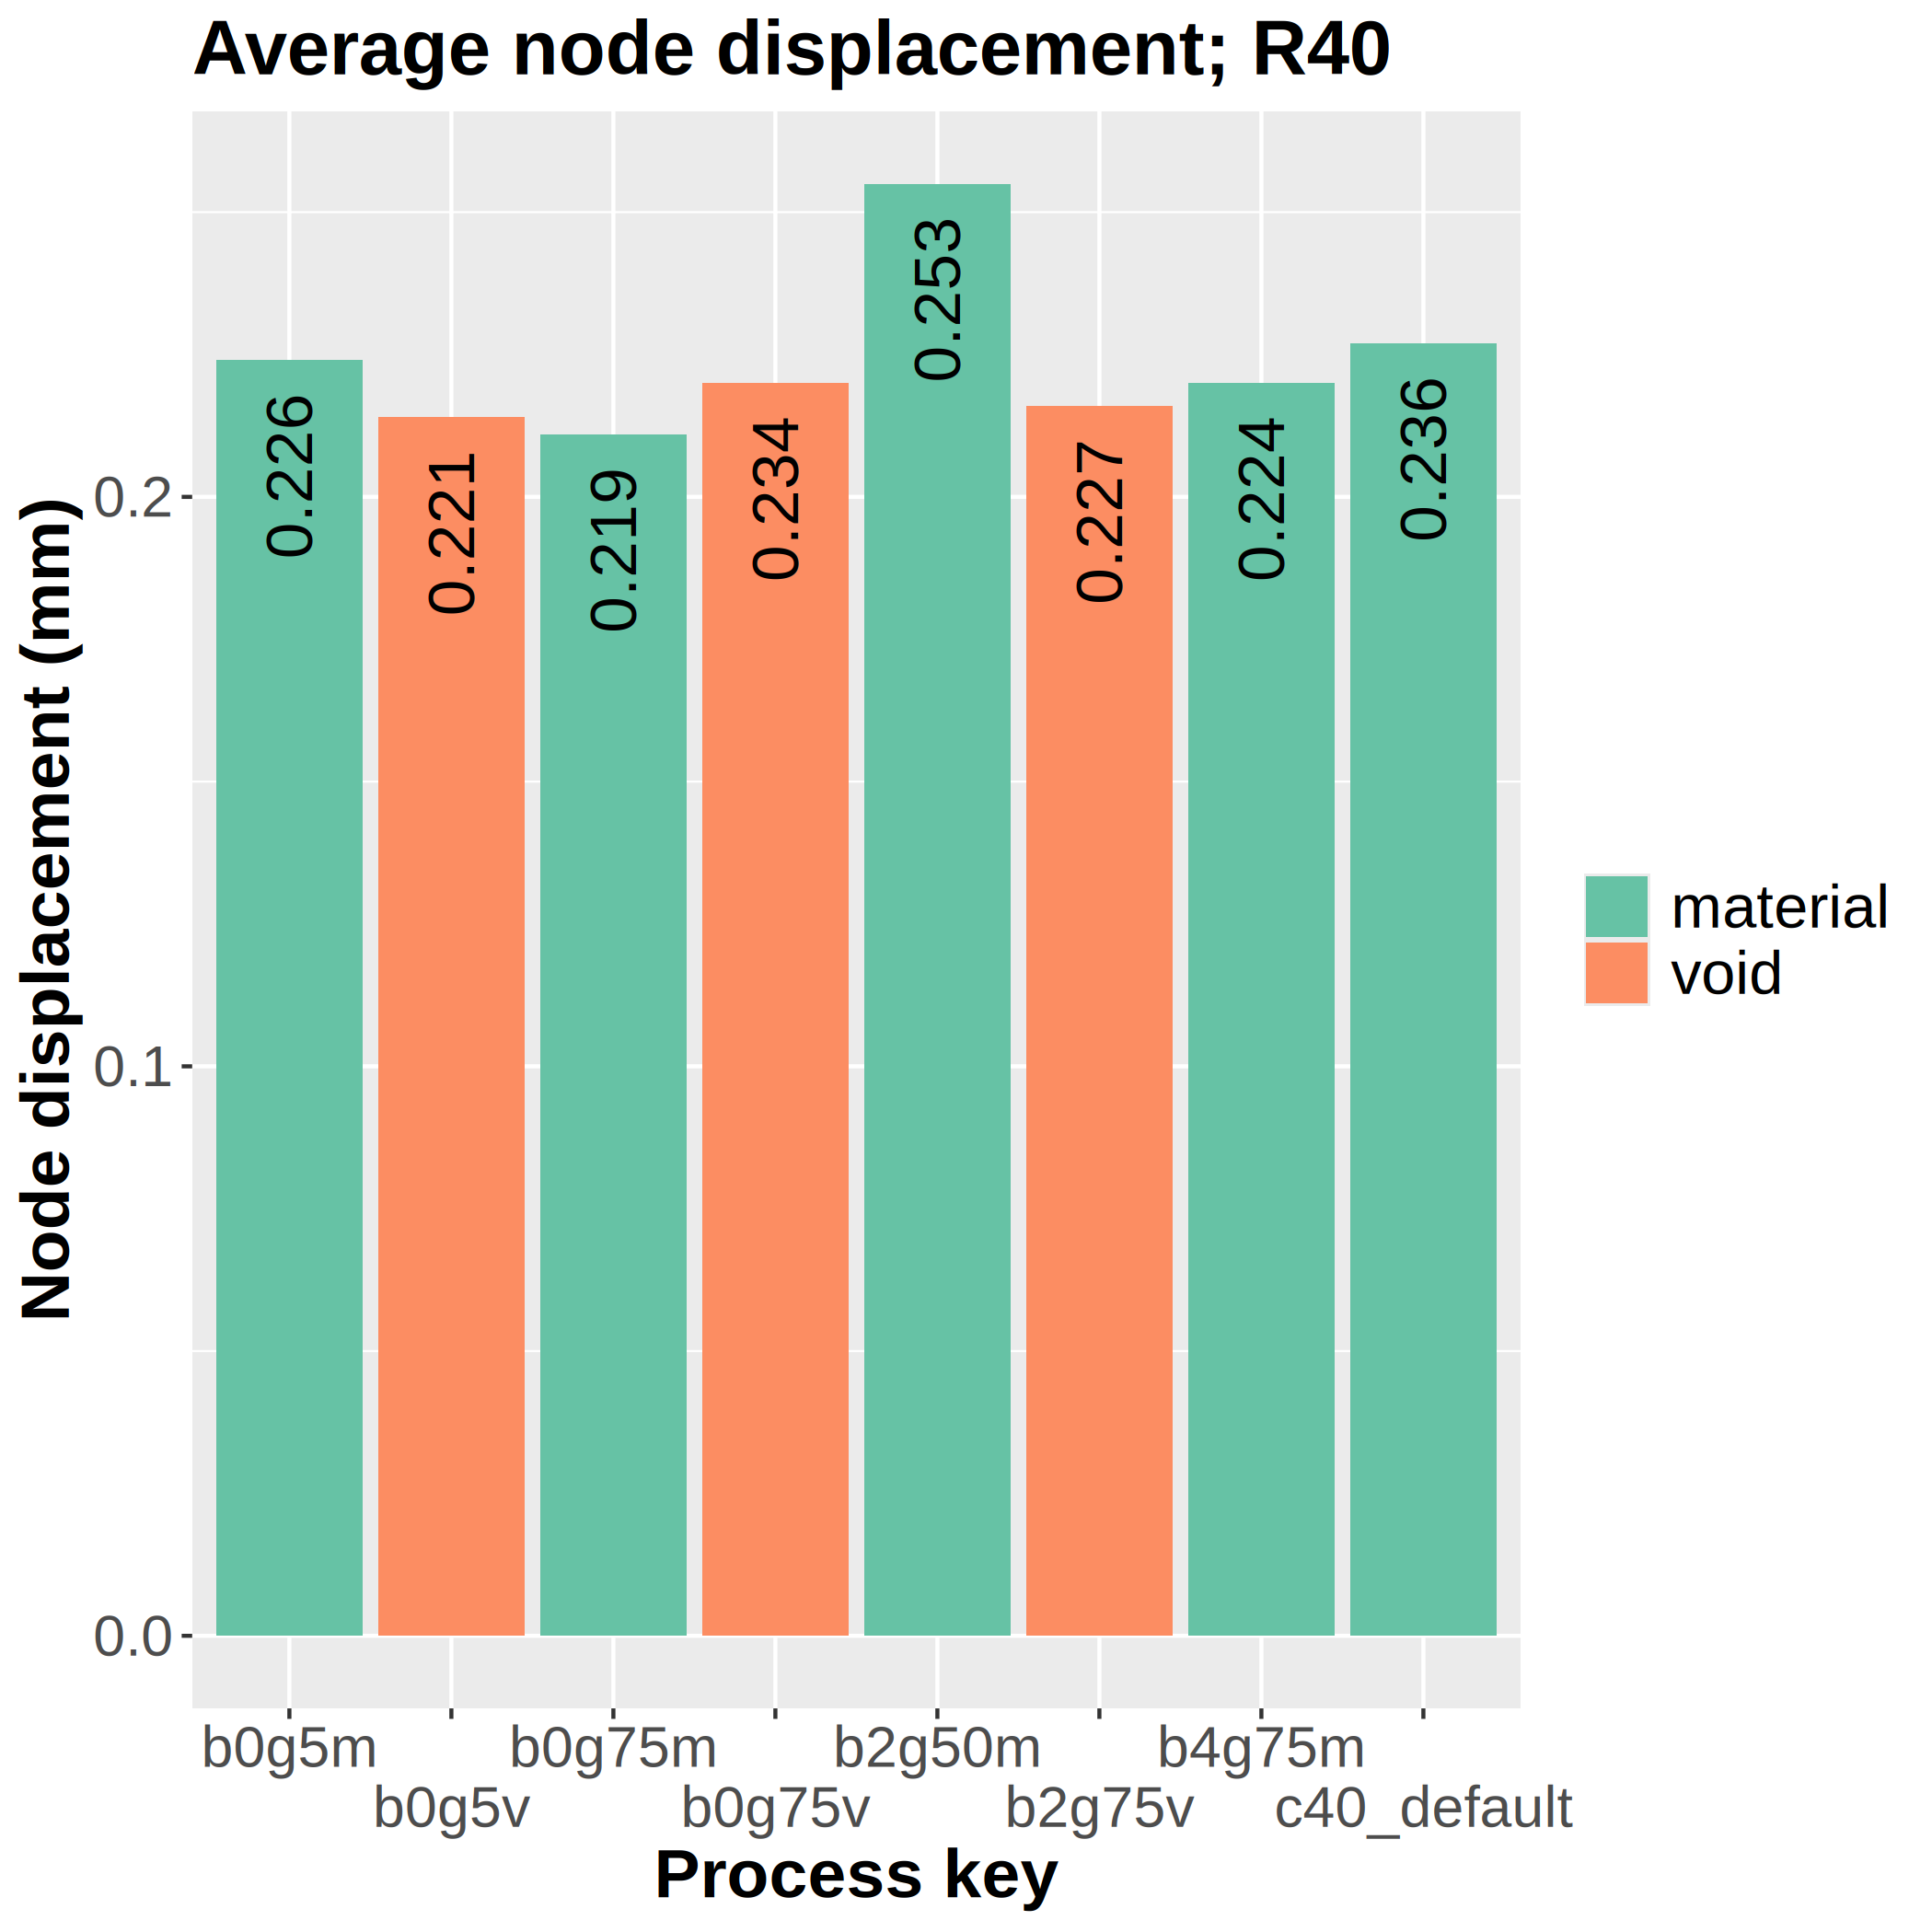
\includegraphics[width=\textwidth]{R40 _disp3.png}
    \label{}
  \end{subfigure}
  \begin{subfigure}[b]{0.45\textwidth}
    \centering 
    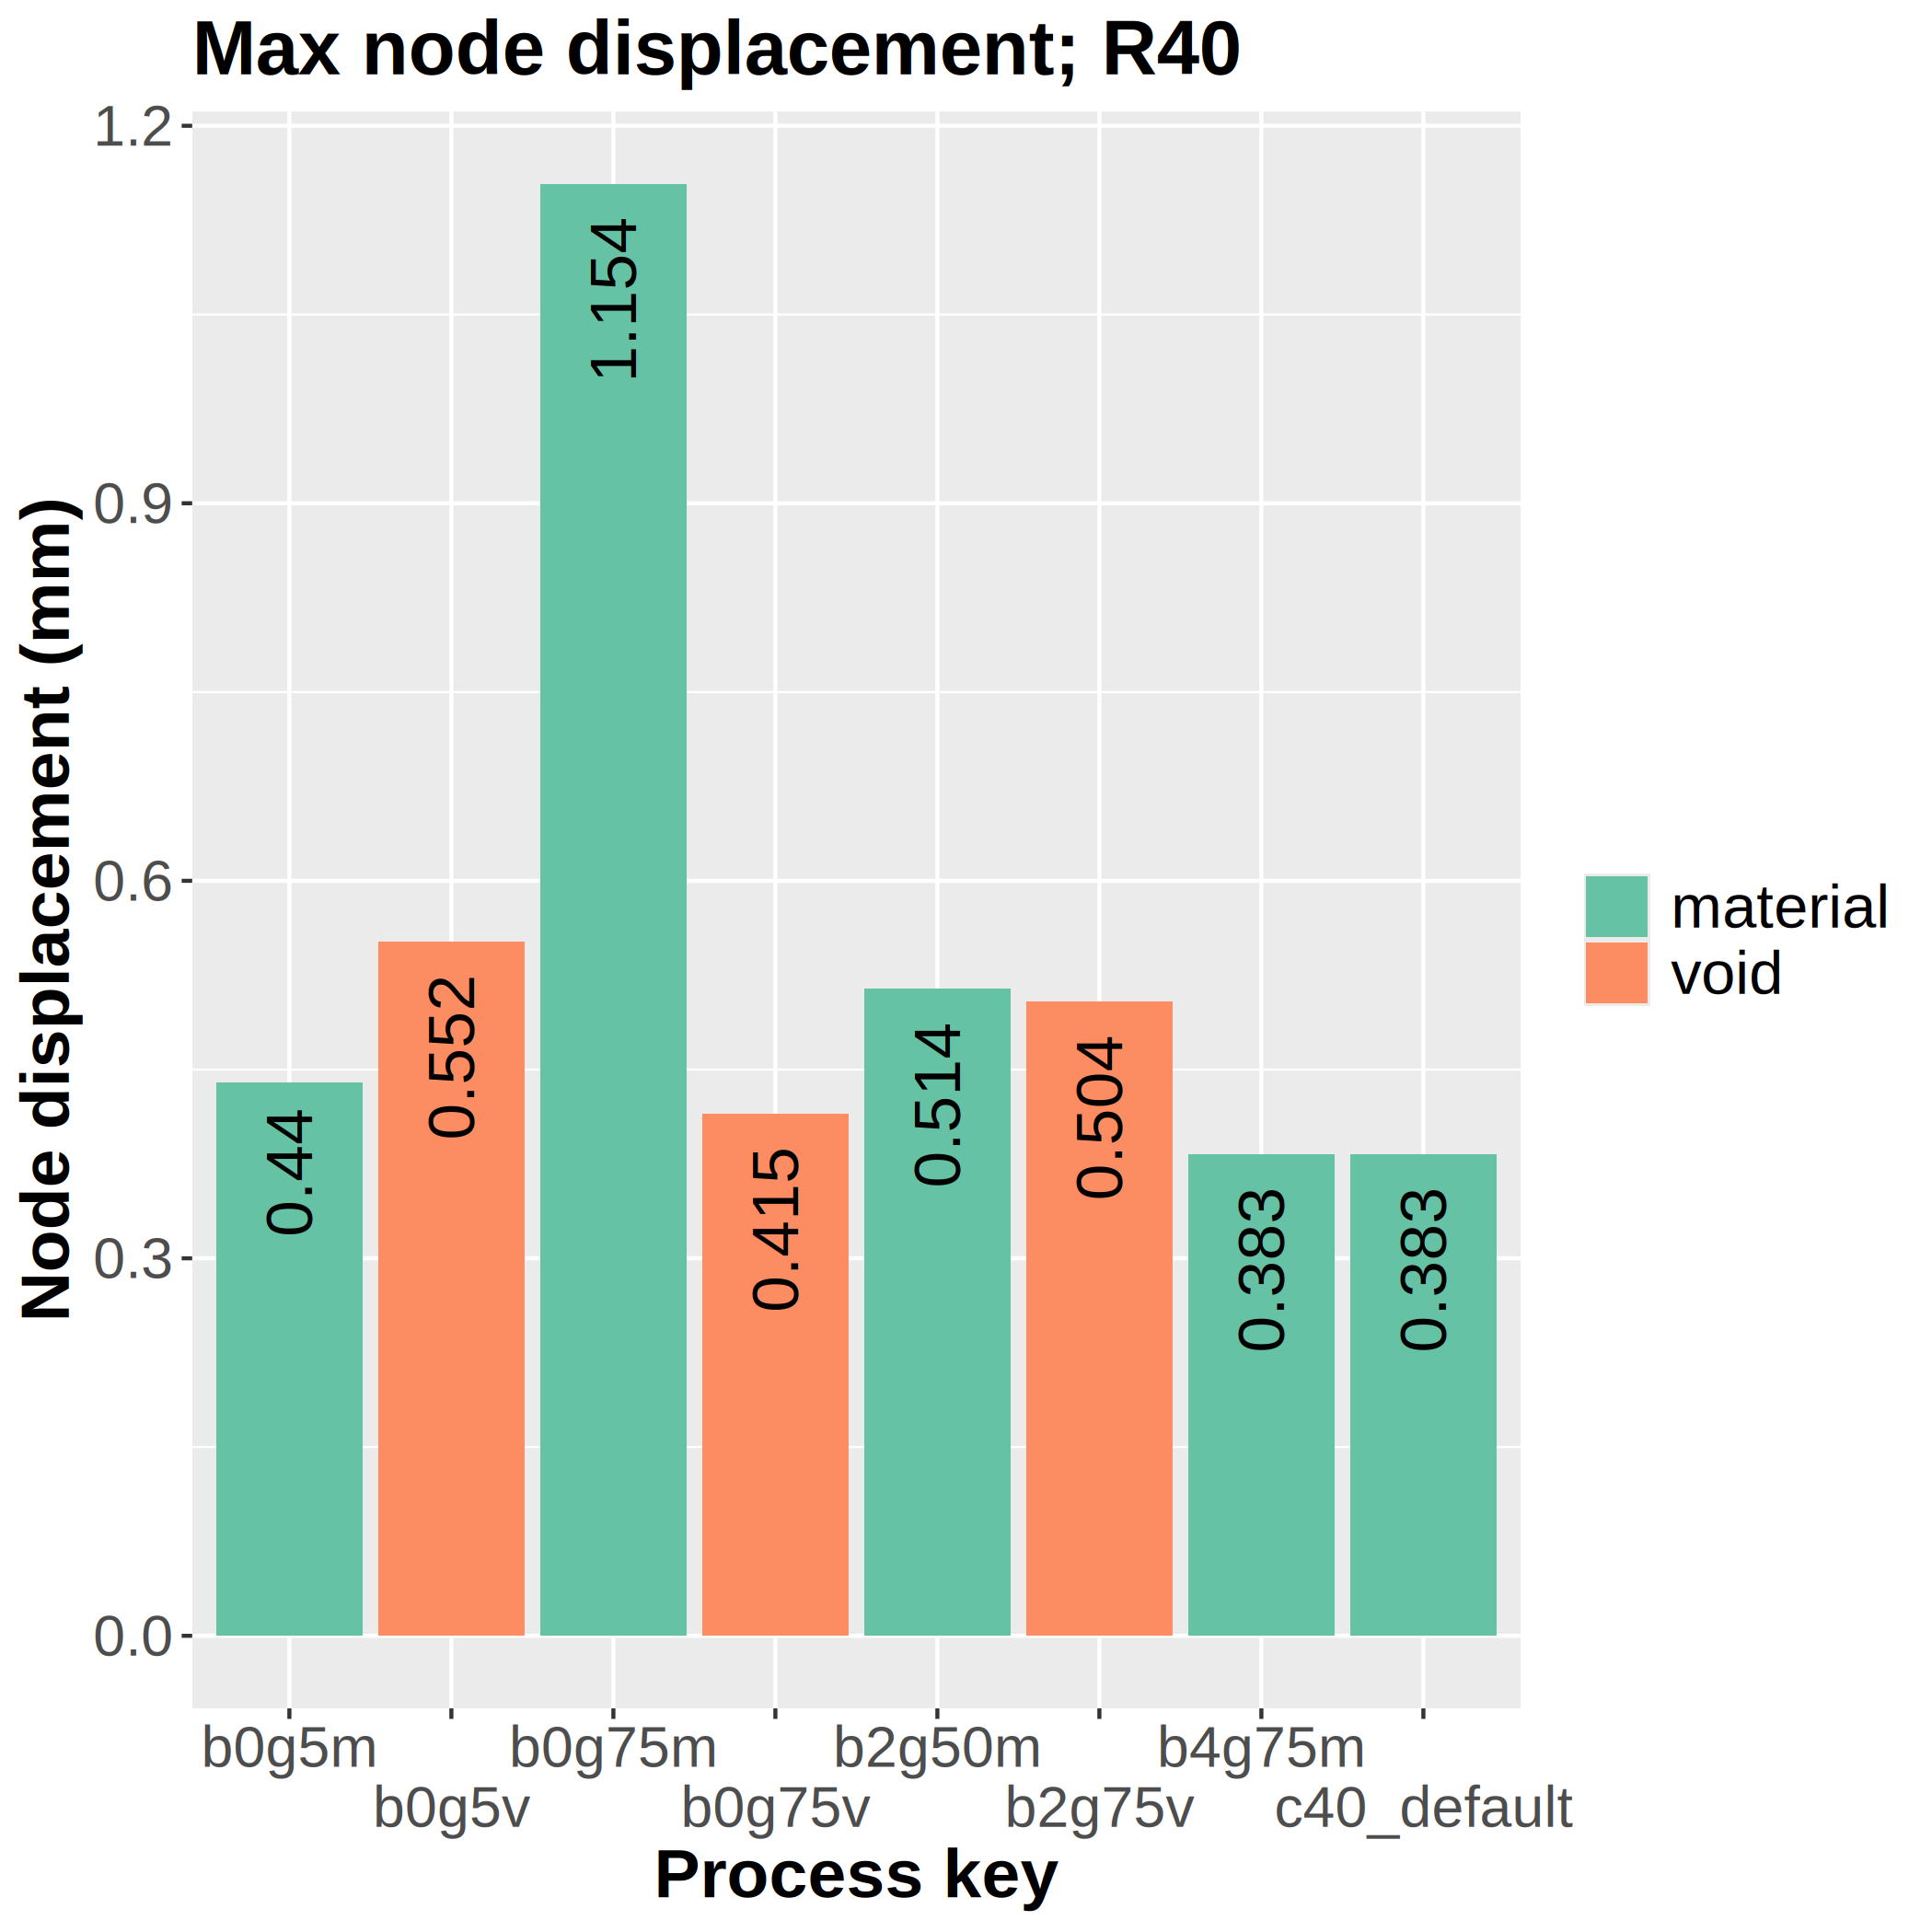
\includegraphics[width=\textwidth]{R40 _dispmax3.png}
    \label{}
  \end{subfigure}
  \begin{subfigure}[b]{0.45\textwidth}
    \centering 
    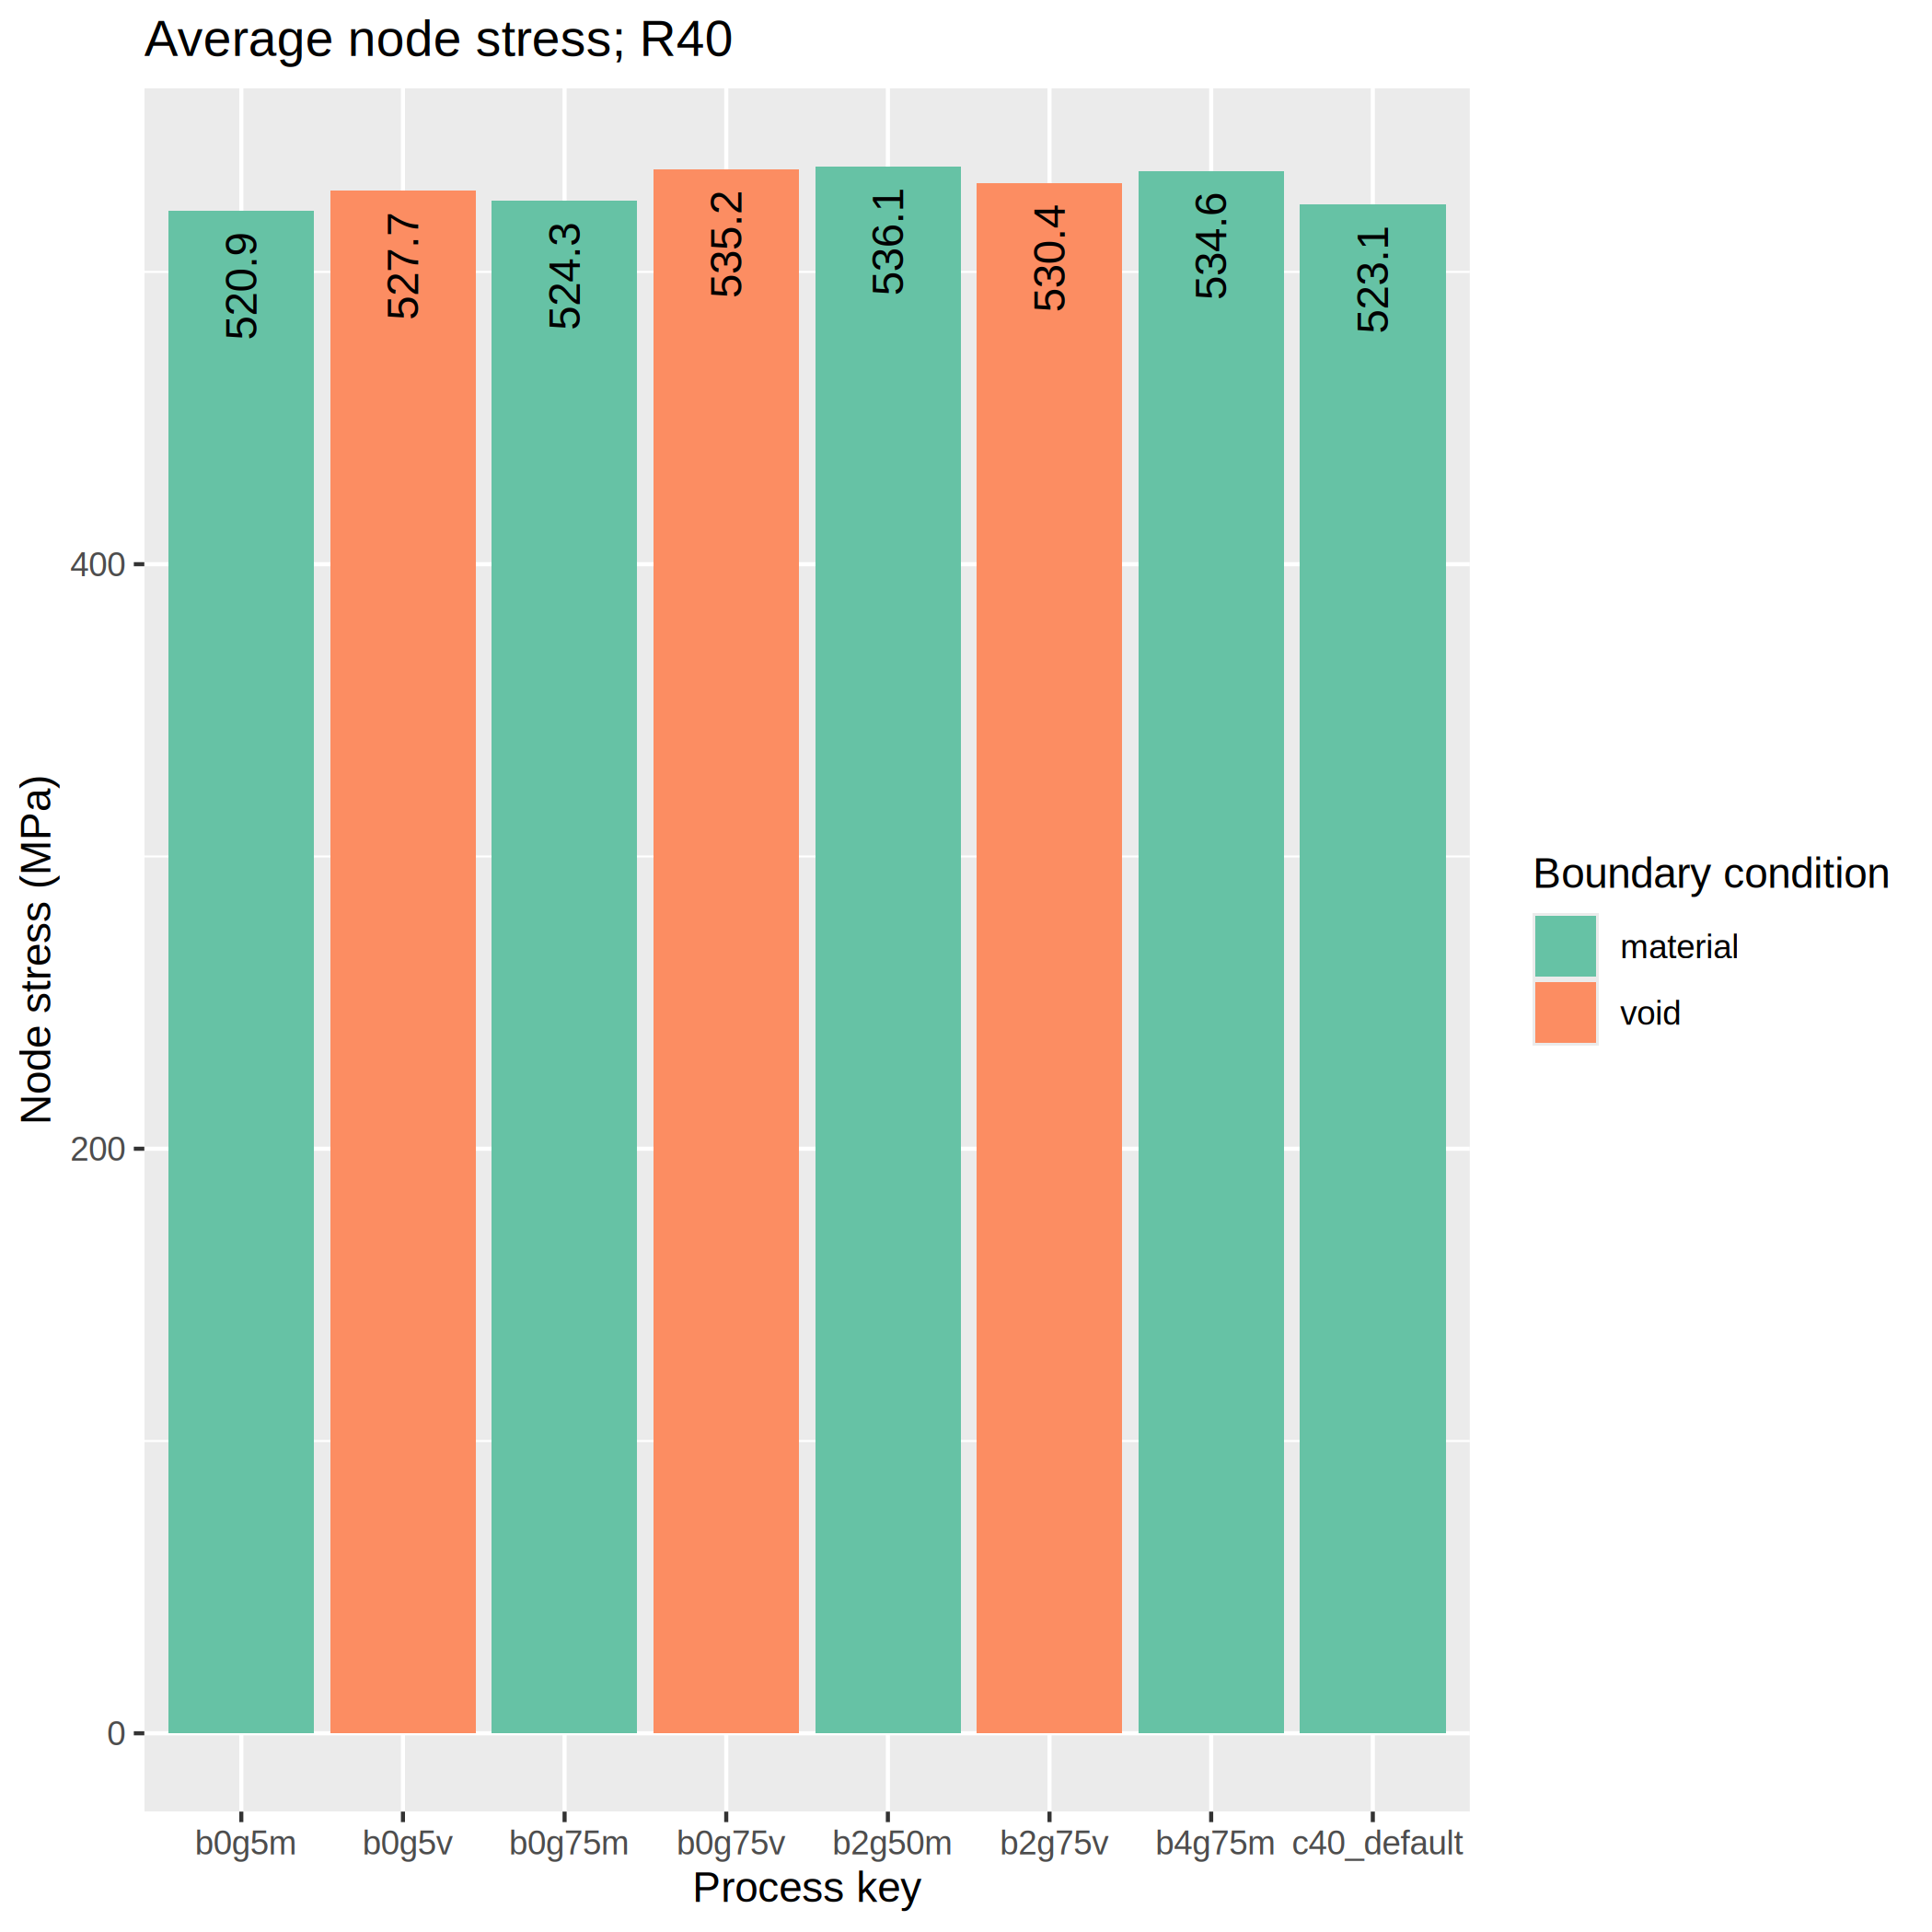
\includegraphics[width=\textwidth]{R40 _stress3.png}
    \label{}
  \end{subfigure}
  \begin{subfigure}[b]{0.45\textwidth}
    \centering 
    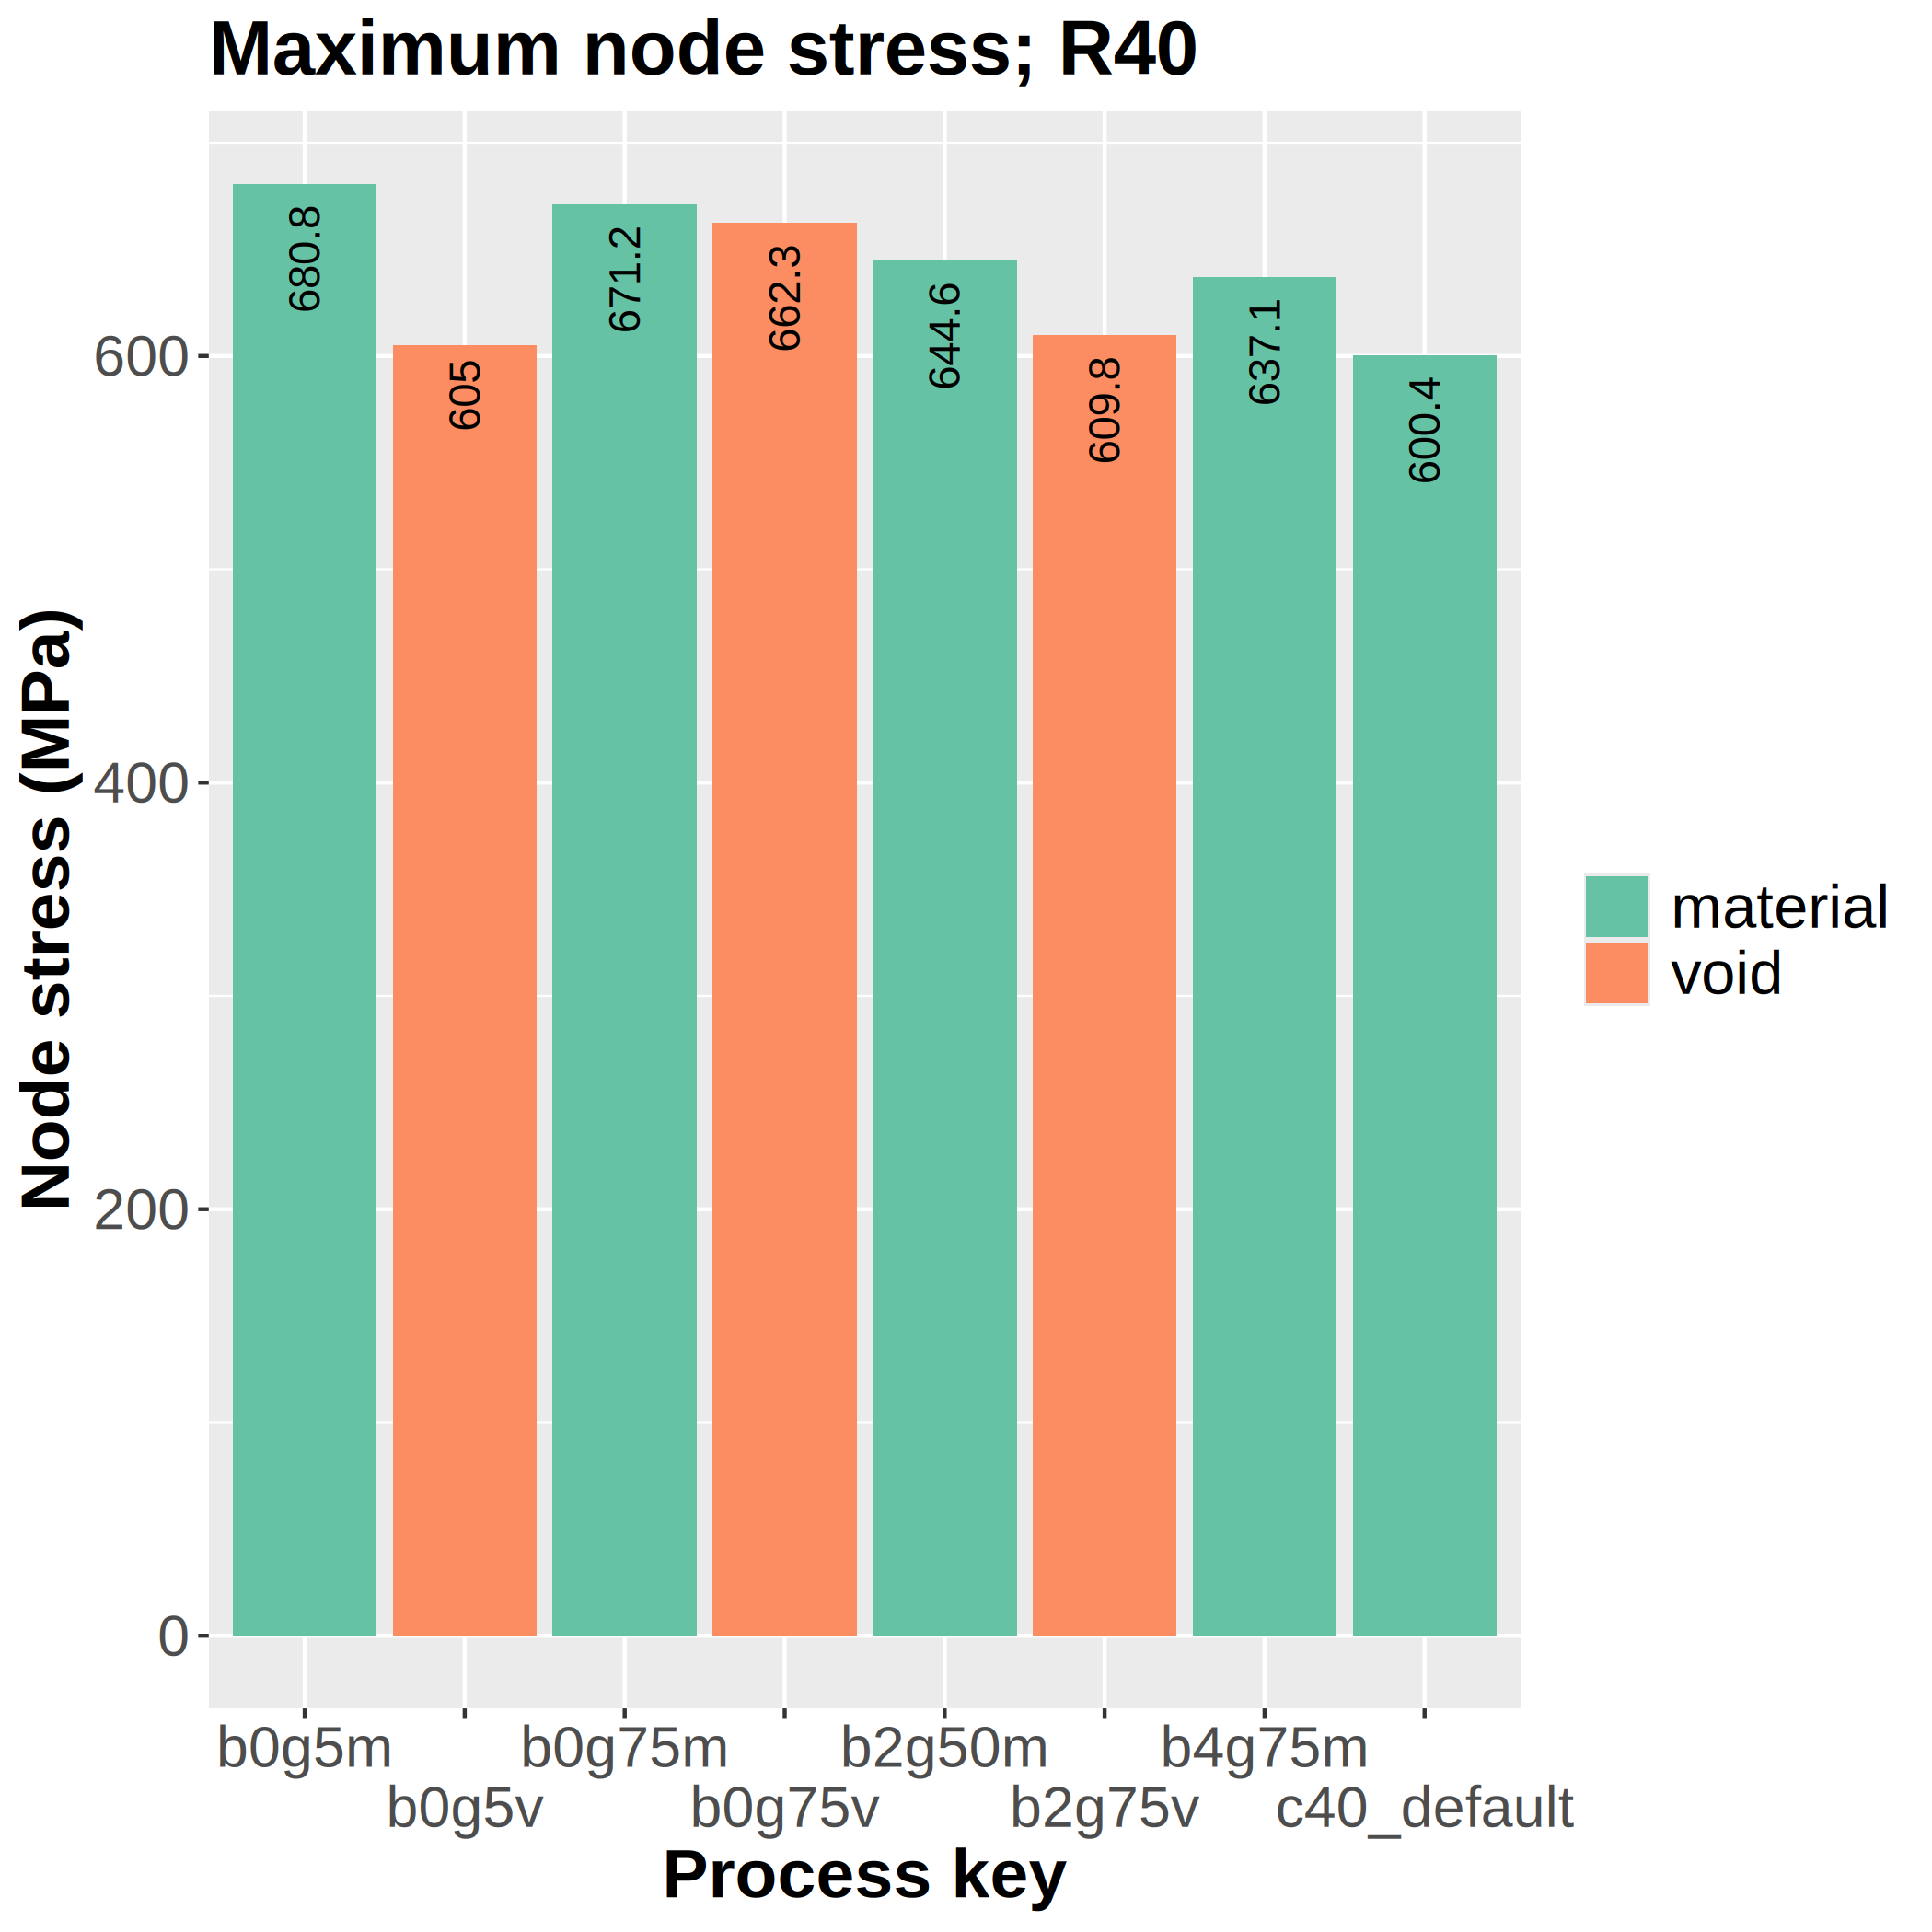
\includegraphics[width=\textwidth]{R40 _stressmax3.png}
    \label{}
  \end{subfigure}
  \caption{Results of 40R fillet.}
  \label{fig:40r_results}
\end{figure}

In summary, the results of these simulations suggest that varying the objective function parameters in the COMSOL simulations did not result in any noticeable differences in the resulting topologies. This suggests that the choice of objective function had little impact on the final structural configurations. Upon closer examination, it was found that the thermal compliance, rather than the mechanical compliance, was the dominant factor driving the topology optimization. This indicates that for the given loading conditions, where the primary load is the weight of the component itself, the mechanical compliance does not play a significant role in the optimization process. The thermal effects appear to be the governing factor, likely due to the relatively low magnitude of the mechanical loads. These findings suggest that a multi-objective function approach may not be necessary for this particular study, as the thermal compliance alone seems to be the primary driver of the optimal topologies. This simplification could be advantageous for future design optimization efforts, as it reduces the complexity of the problem and allows for a more focused exploration of the thermal-driven structural behavior.

\clearpage

\section{Results of femoral components}

\subsection{Displacement analysis}

For the displacement analysis of the femoral component, statistics on the surface mesh of the simulation results were computed. From this graph,  

Figure \ref{fig:disp_ridges} shows the distribution of the surface nodal displacements of the femoral component. The utility of this graph is to visualize easily how the displacements of each result are distributed. We see that the distribution is asymmetrical and it does not resemble a normal distribution. From the other graphs, it can also be observed that the hyperbolic tangent variation within volume fraction group creates slight differences in the distribution of nodal displacements, although it seems only to occur in some particular cases. Lastly, it can be seen from these graphs that the lower volume fractions of 25\% and 33\% have slightly thicker right-end tails, suggesting that there is a greater number of nodes with high displacement as compared to the other simulations.

\begin{figure}[h!]
  \centering
  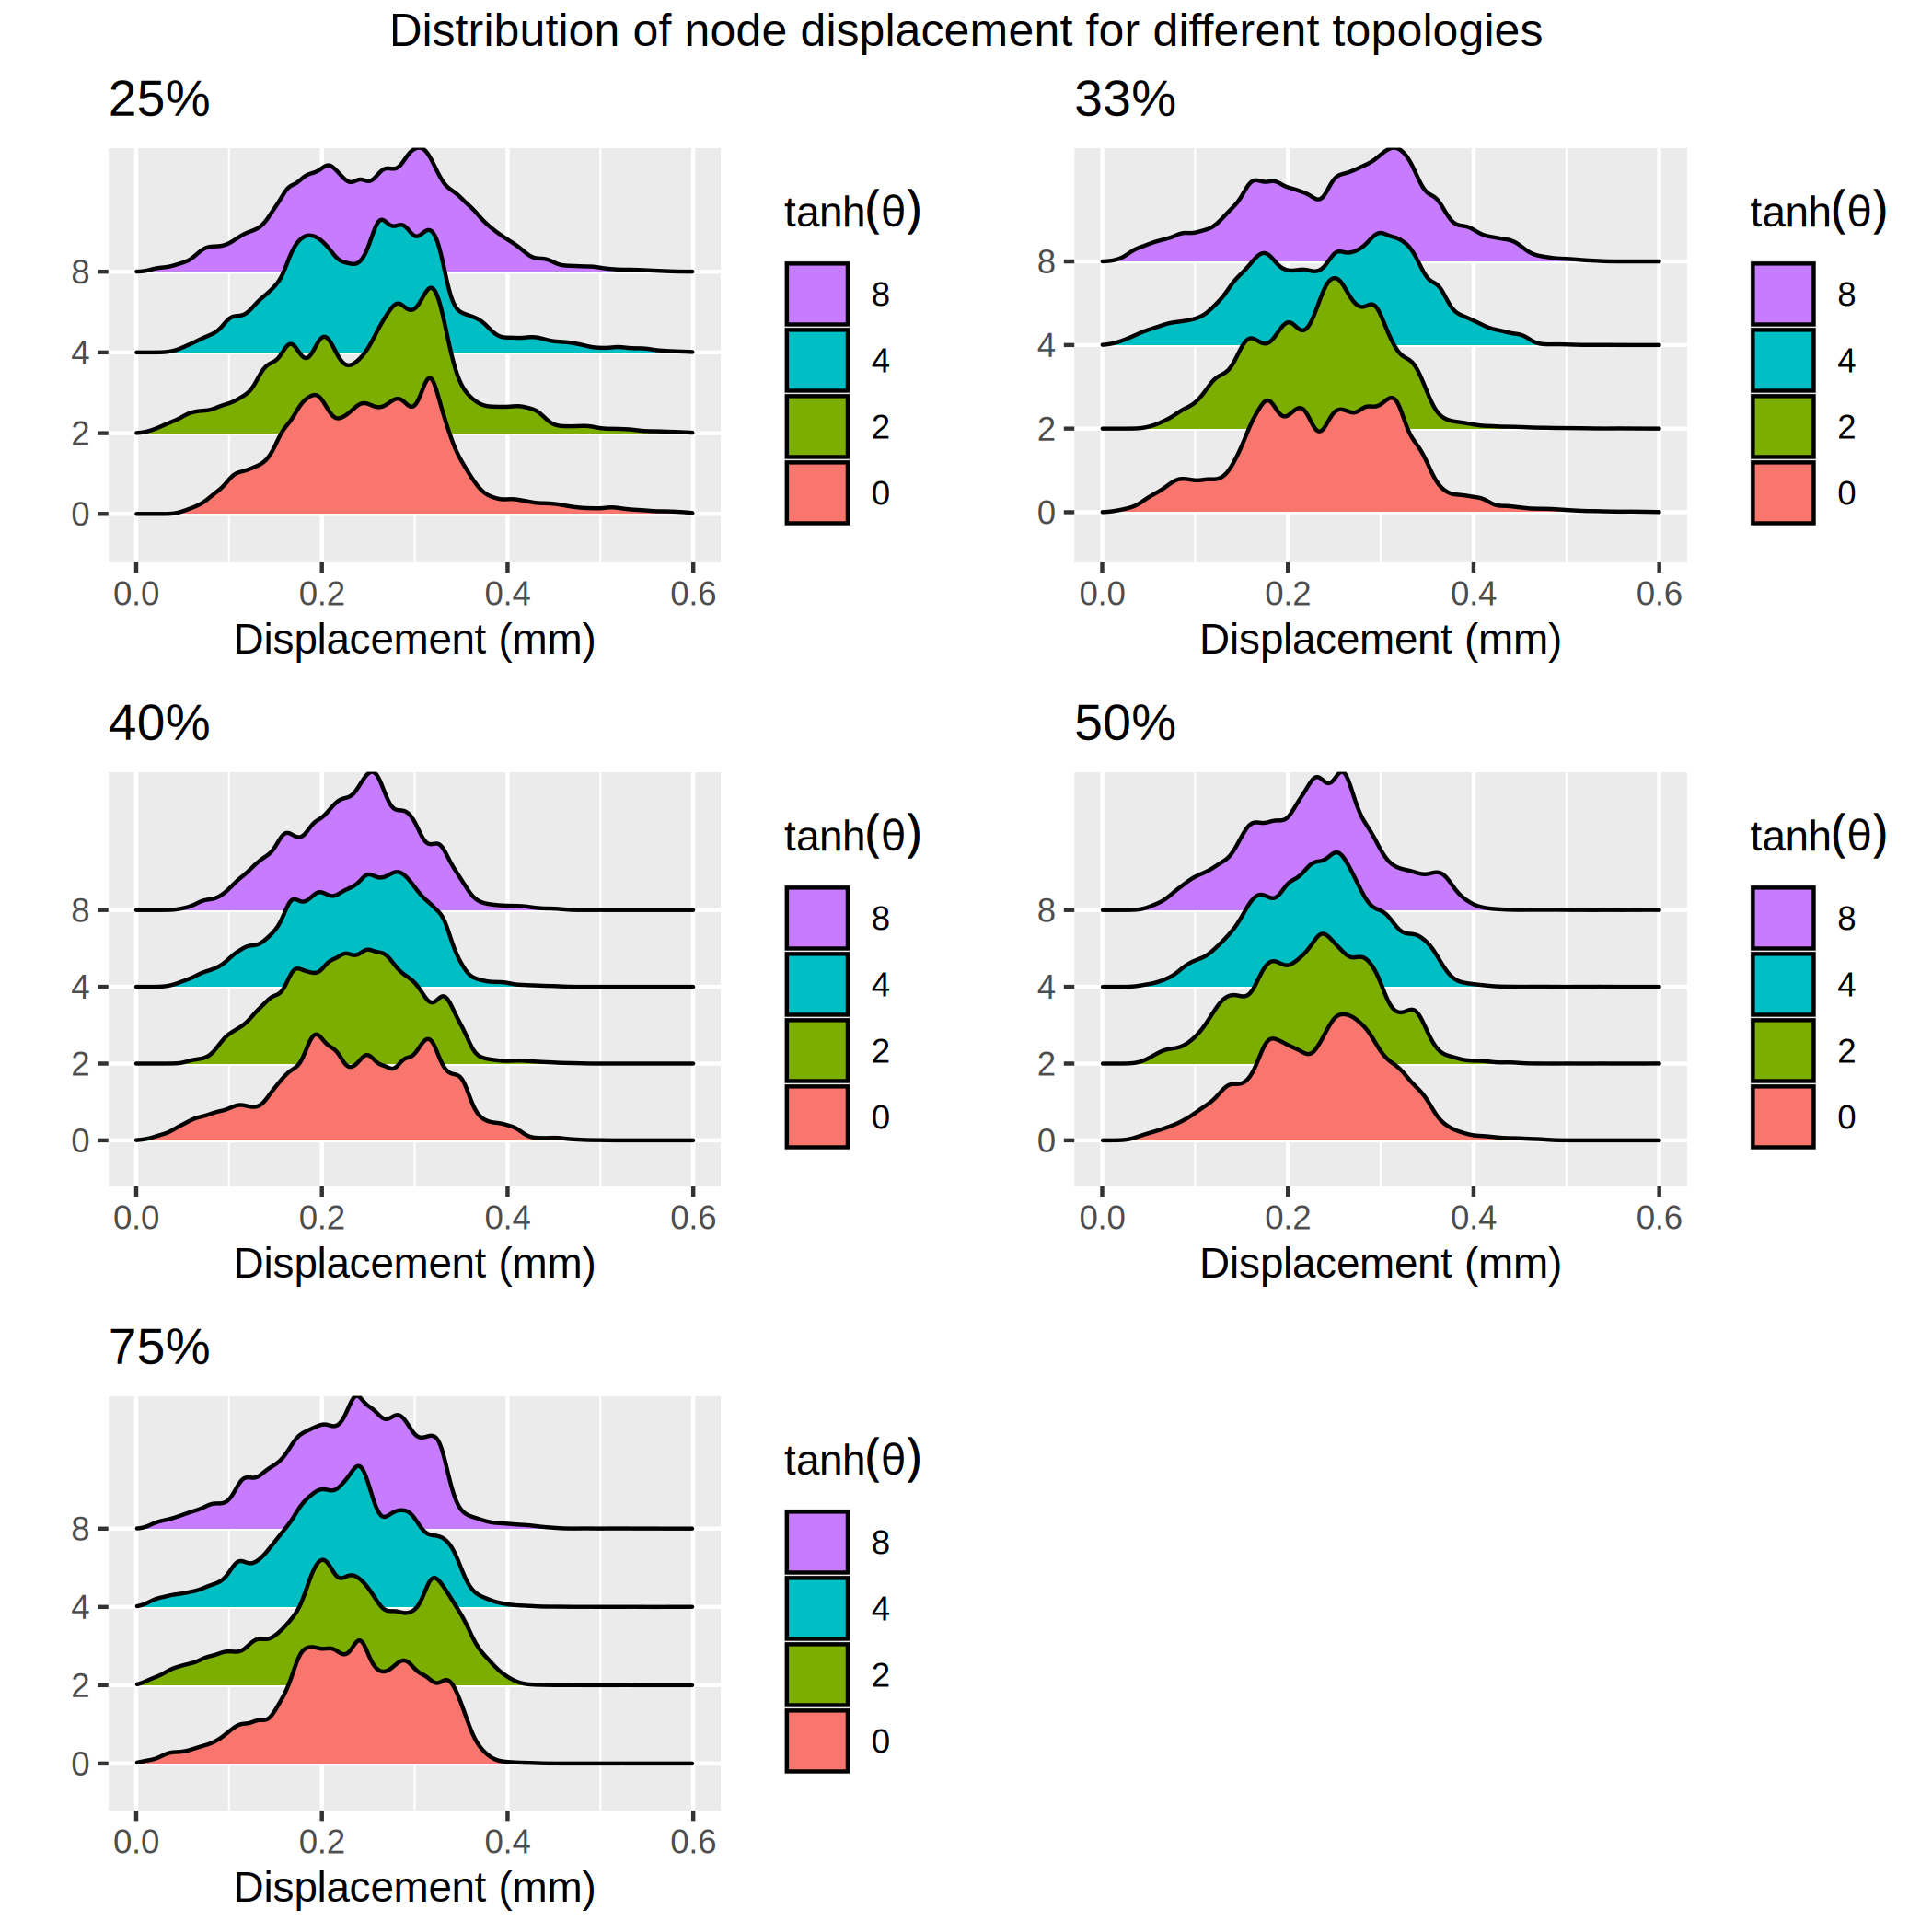
\includegraphics[width=0.9\textwidth]{images/results/plots/femoral/displacement/disp_density_ridges.png}
  \caption{Density distribution of nodal displacements, grouped by volume fraction and hyperbolic tangent angle.}
  \label{fig:disp_ridges}
\end{figure}

This trend can be more easily visualized by computing the average nodal deformation for each case. The left graph of Figure \ref{fig:disp_averages} shows the average nodal deformation, where each column corresponds to a simulation result and each color represents a particular volume fraction group. It is clear from this graphs that the 25\% and 33\% volume fraction results exhibit a slightly larger average deformation compared to the rest of the simulations. This is more clearly show in the right figure, which shows the average deformation for each volume fraction group as a whole. Nevertheless, this difference between average nodal deformation could still be attributed to the numerical uncertainty due to voxelization, as it had been previously established that the numerical errors of the simulation could account up to a variability of 0.01mm.

\begin{figure}[h!]
  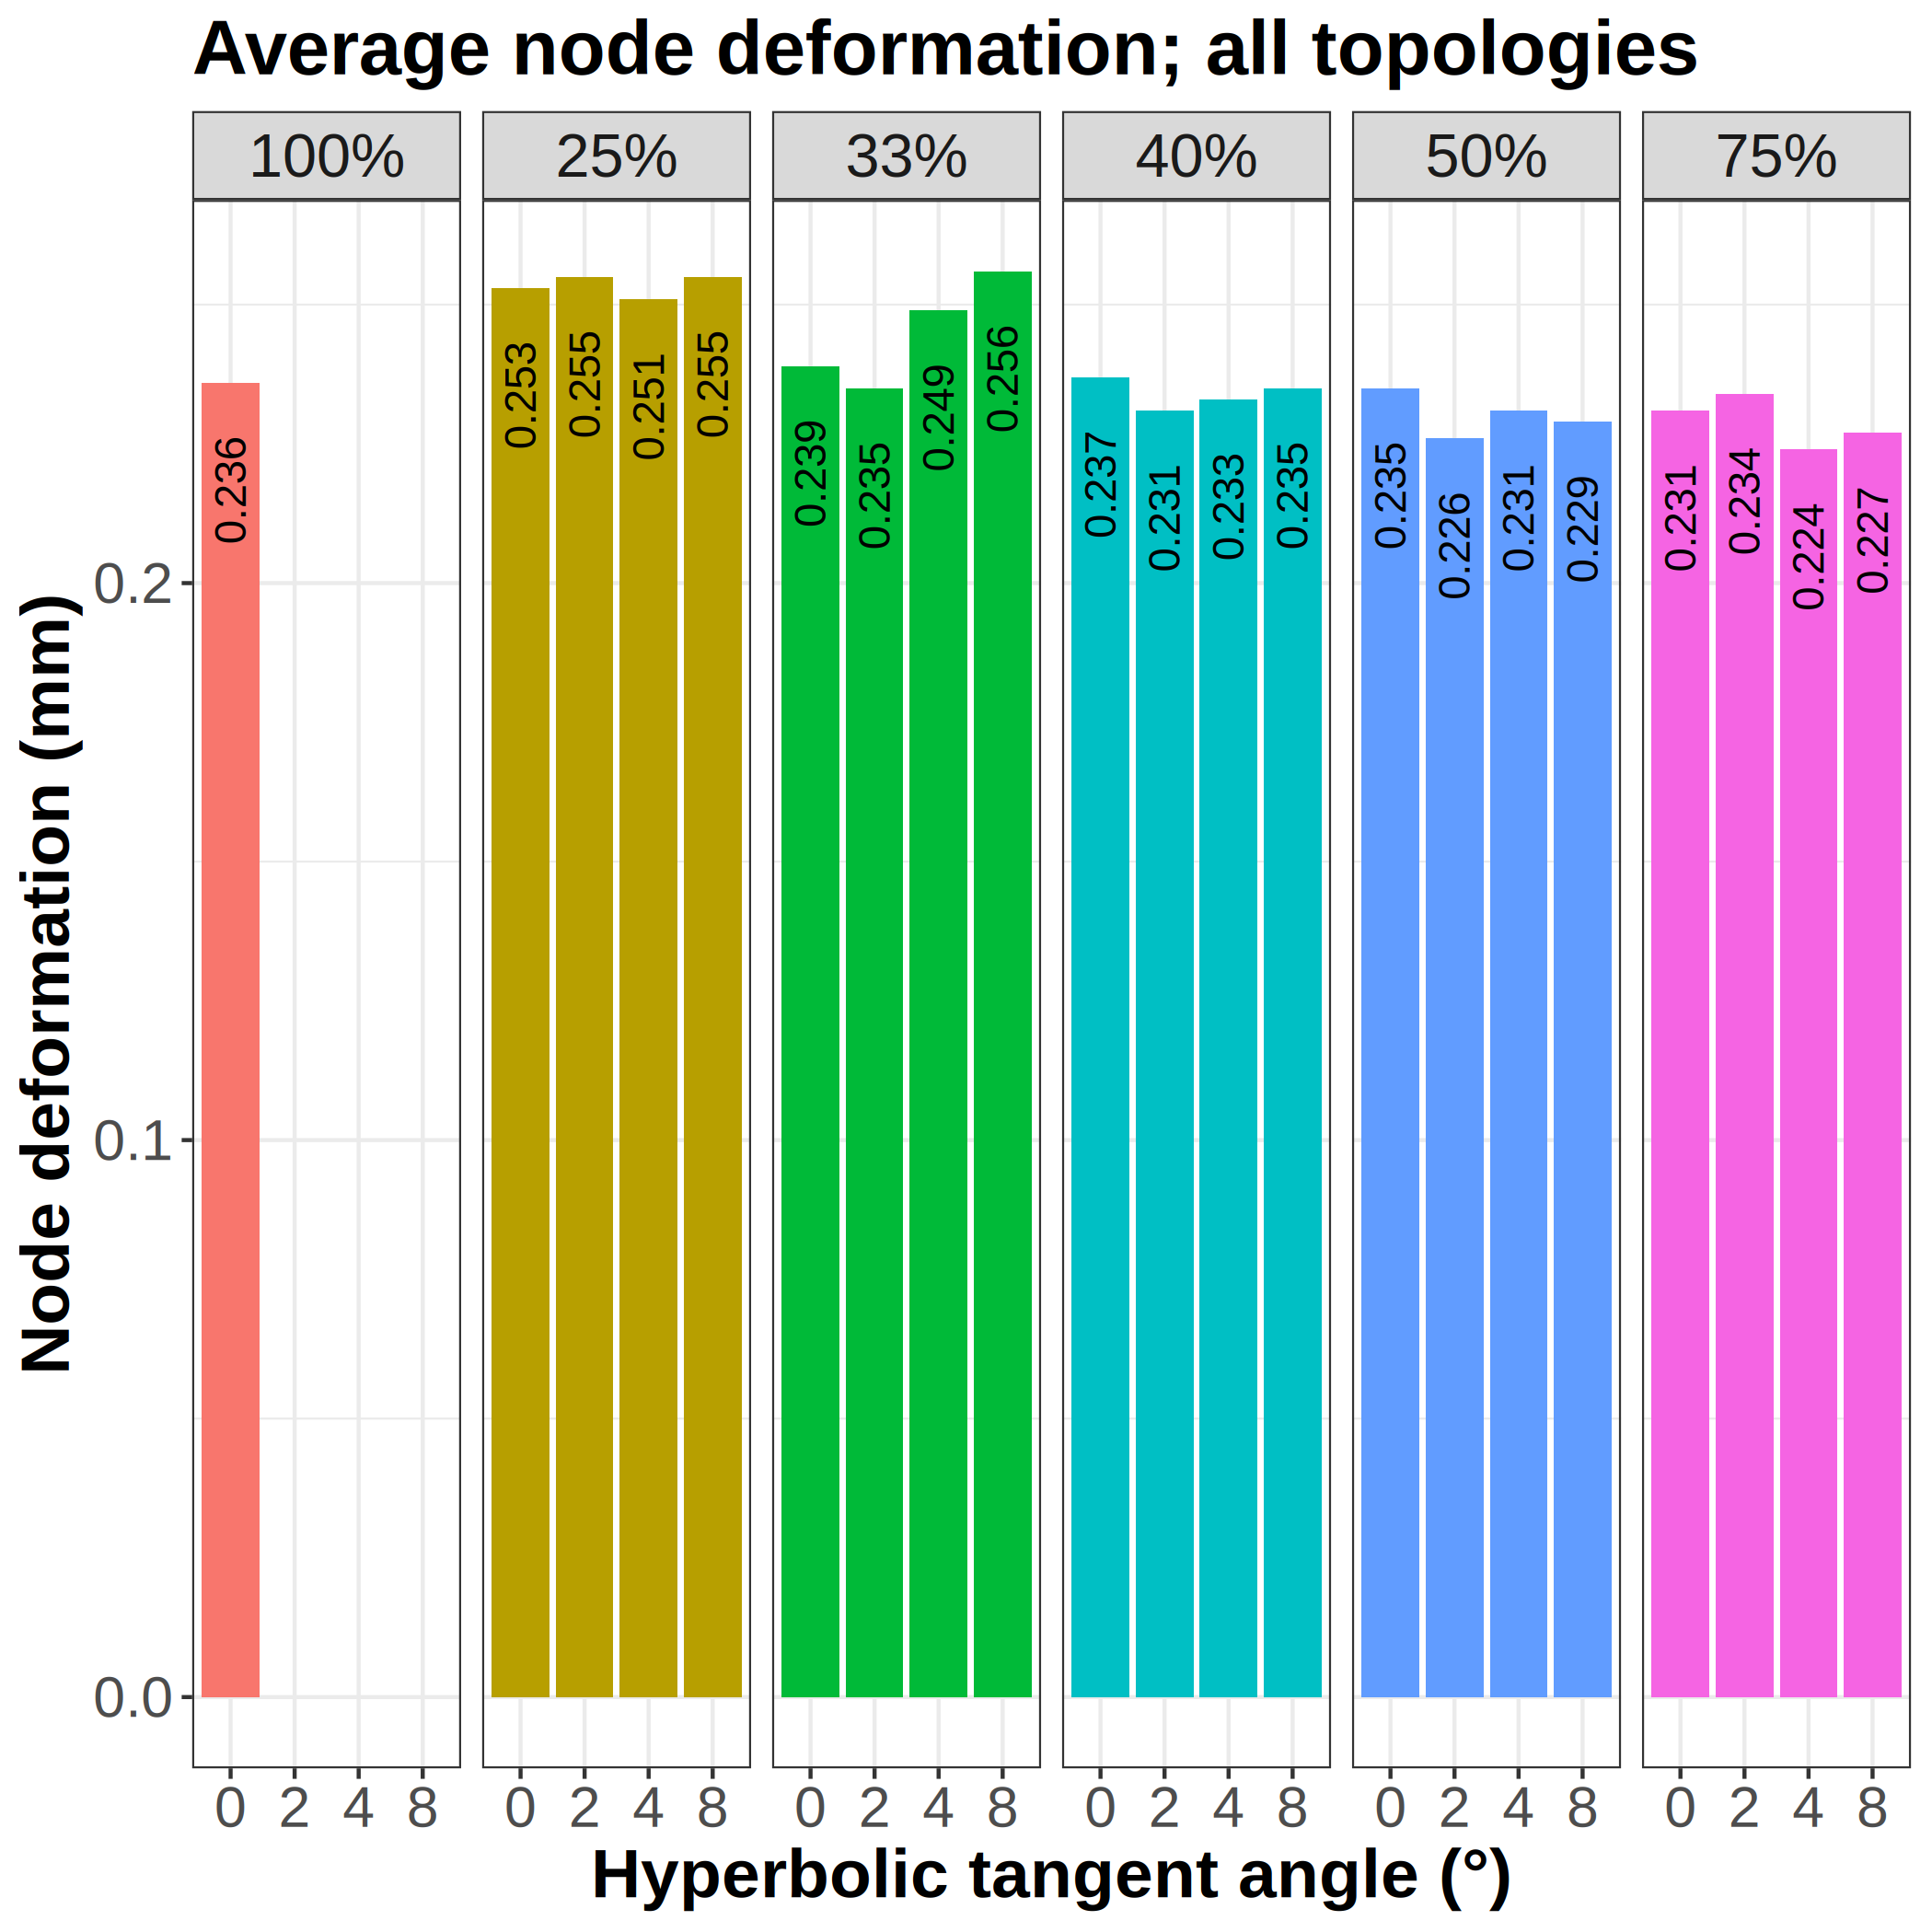
\includegraphics[width=0.45\textwidth]{images/results/plots/femoral/displacement/femoral_average.png}
  \hfill 
  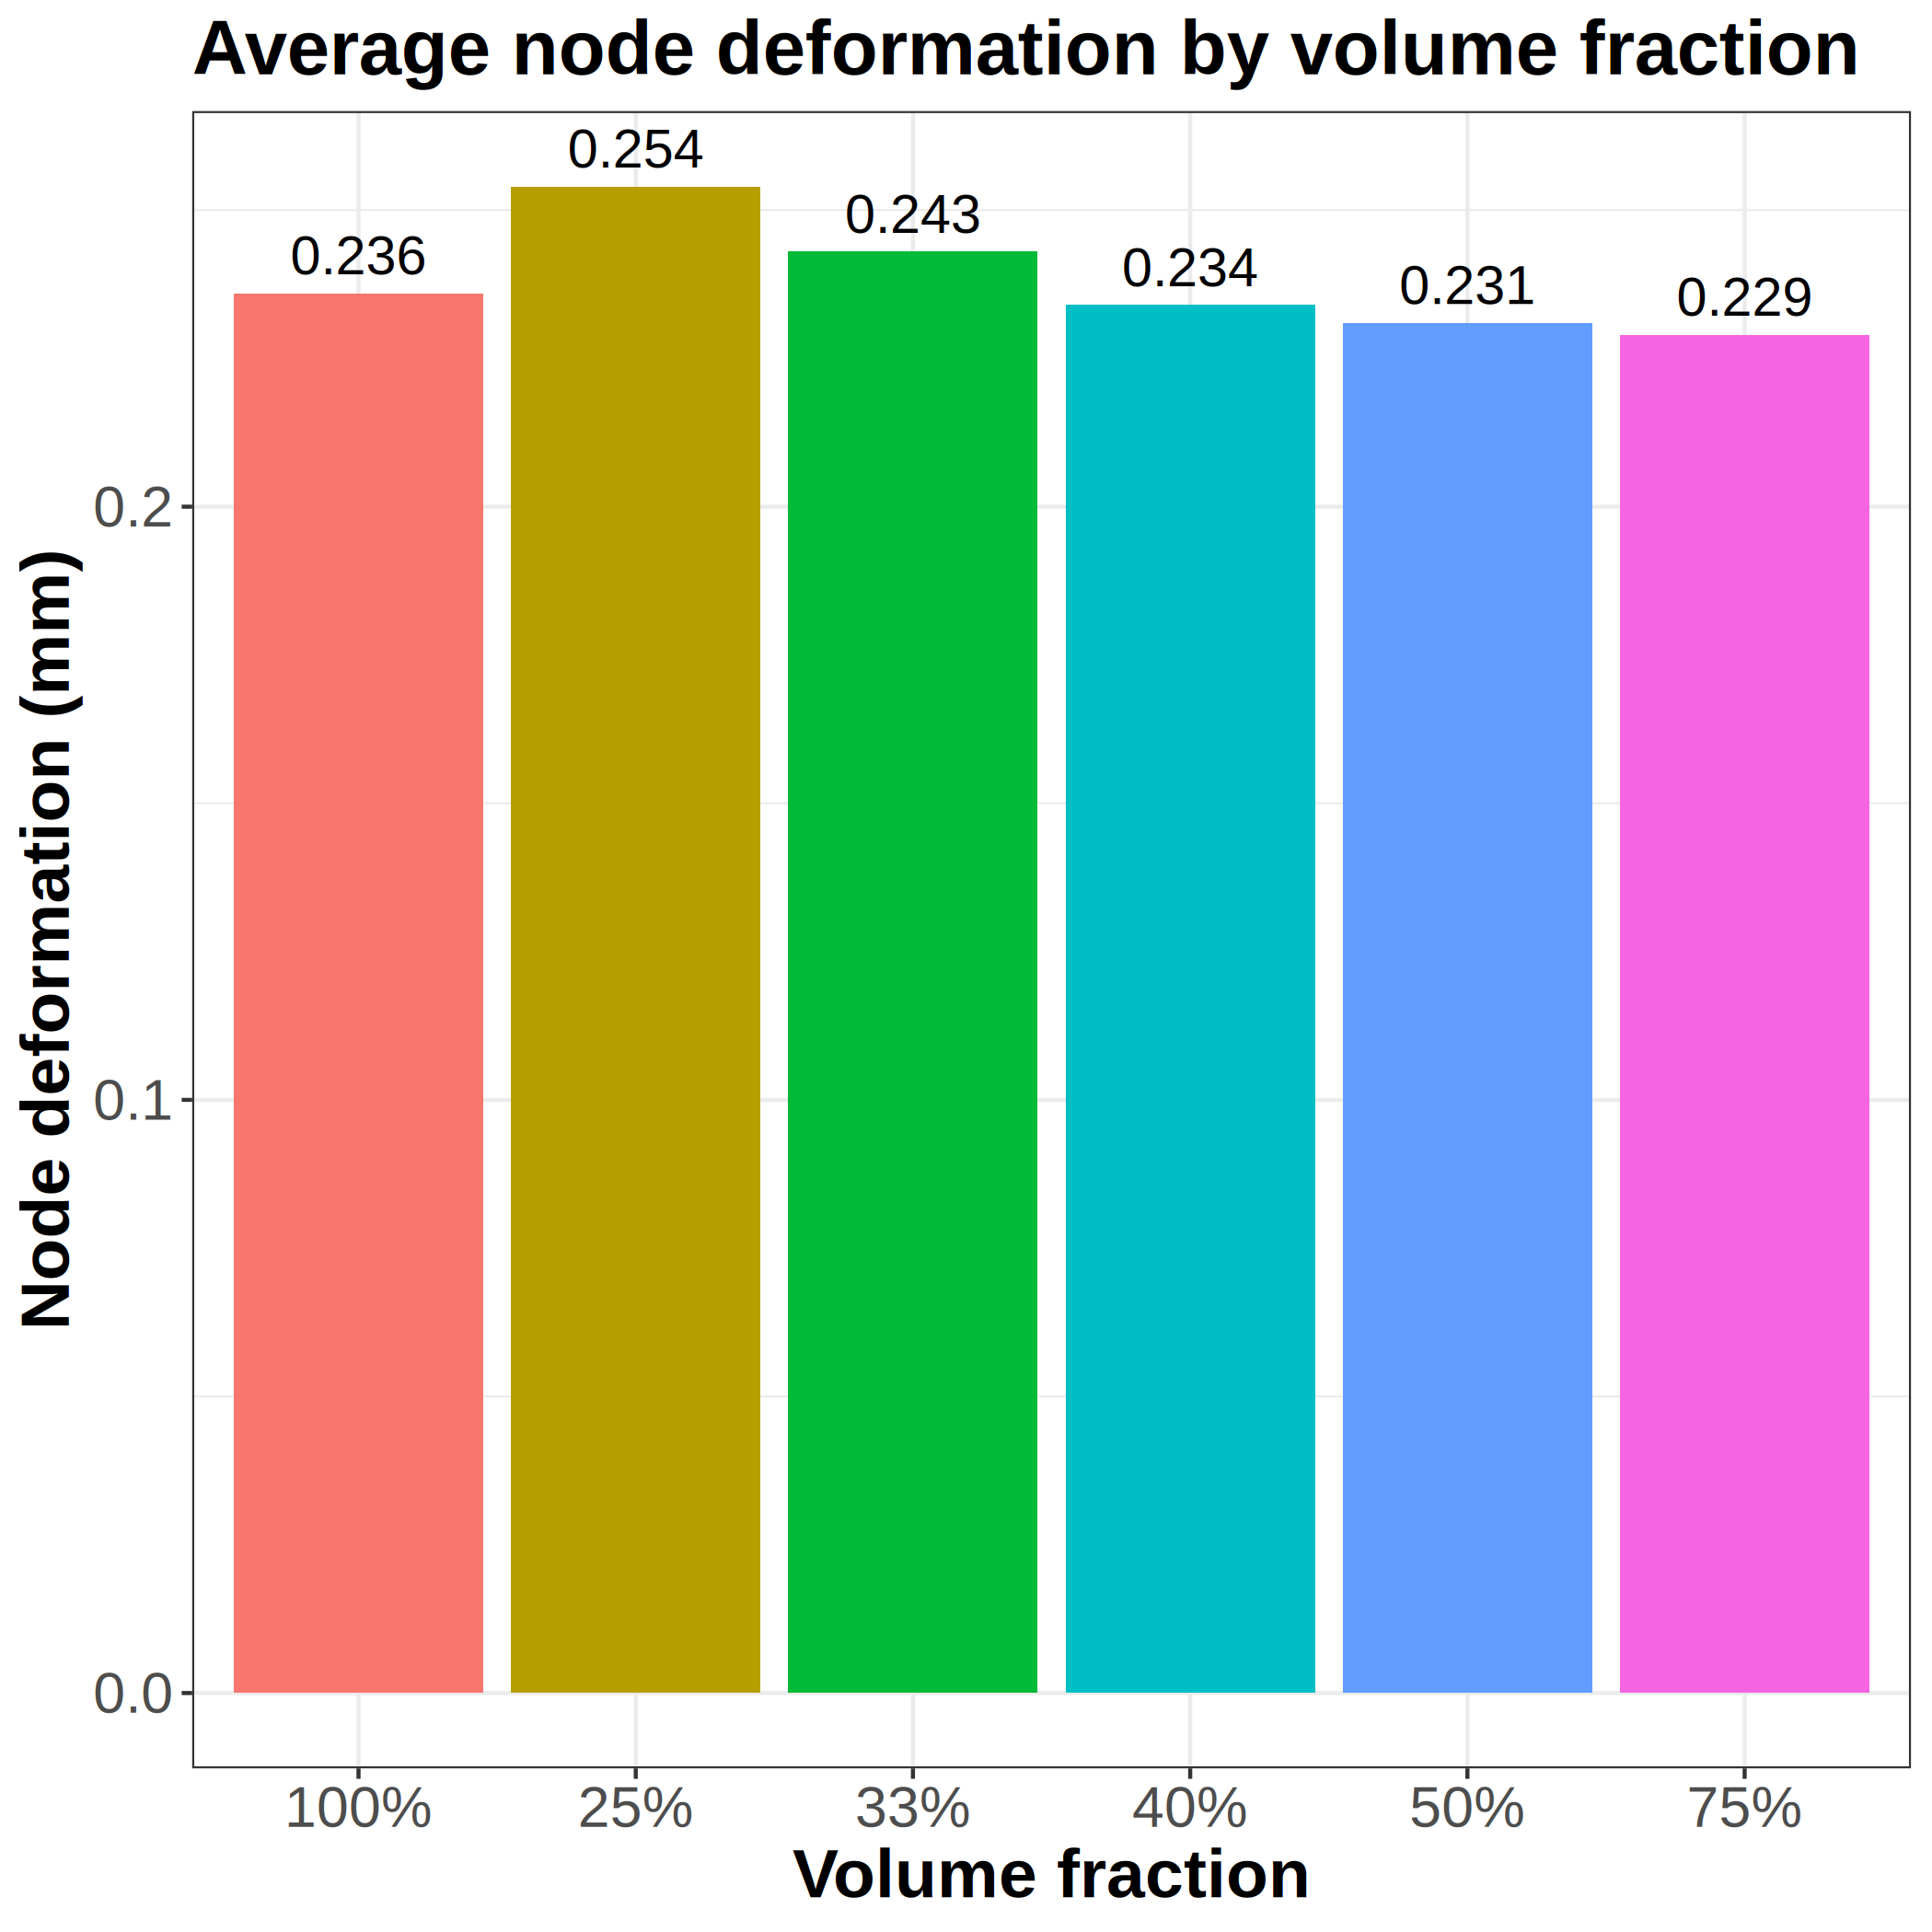
\includegraphics[width=0.45\textwidth]{images/results/plots/femoral/displacement/femoral_average_group.png}
  \caption{Average nodal displacement for femoral component simulations. The left graph shows the average deformation for each topology investigated, the right graph shows the average deformation of topologies when grouped by volume fraction.}
  \label{fig:disp_averages}
\end{figure}

Next, the maximum nodal displacements of each group were computed. The results are shown in Figure \ref{fig:disp_max_bad}. There are three results that show excessive deformation at a few nodes. Additionally, it was noticed during the simulation that some voxels exhibited abnormal behavior, and deformed in a non-physical manner. This is showcased in Figure \ref{fig:bad_voxel}, where one voxel has merged into a neighboring one. Therefore, it is highly suspected that the results for these geometries show faulty node displacements caused by a bug or anomaly in the finite element calculation. To determine whether these excessive deformations are significant, the deformation were binned in bins of 0.1 mm. The result of this operation is shown in  Table \ref{table:disp_bins}.

\begin{figure}[h!]
  \centering
  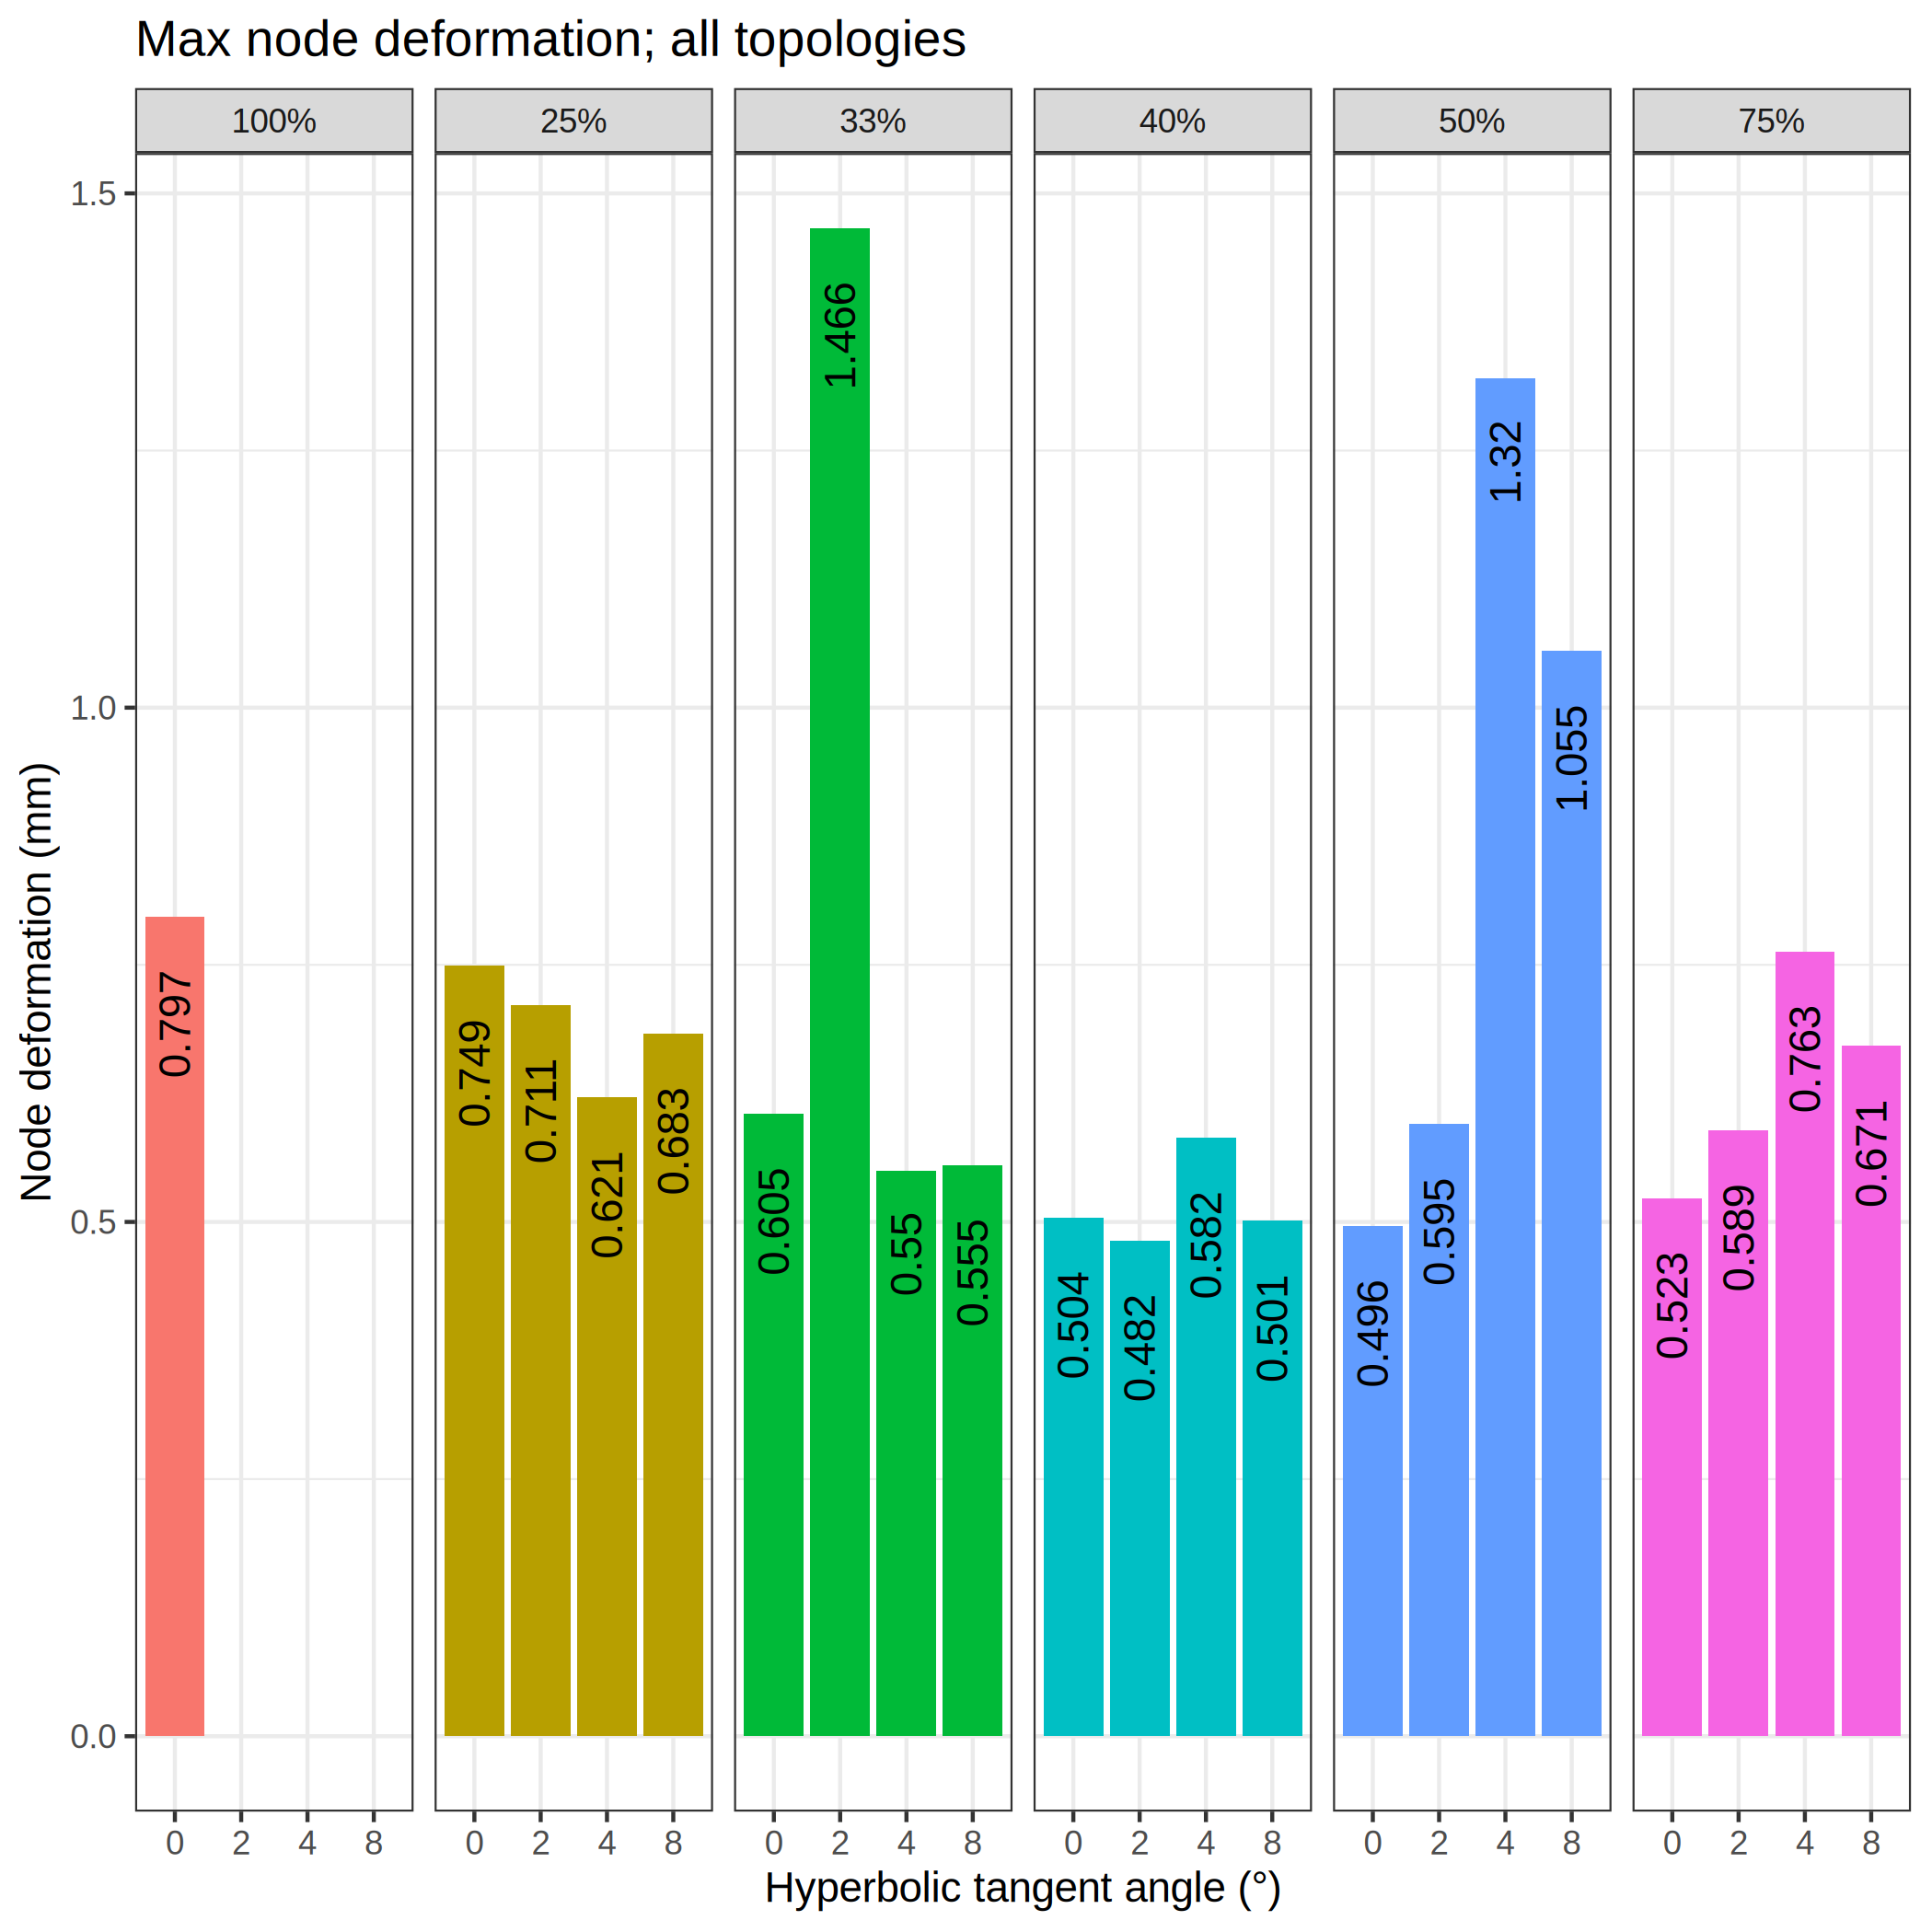
\includegraphics[width=0.6\textwidth]{images/results/plots/femoral/displacement/femoral_max_bad.png}
  \caption{Maximum nodal displacements for the femoral component simulations. Notice that there are three topologies that show an excessive maximal displacement. These displacements are very likely to be outliers, and further analysis was done to understand their nature.}
  \label{fig:disp_max_bad}
\end{figure}

\begin{figure}[h!]
  \centering
  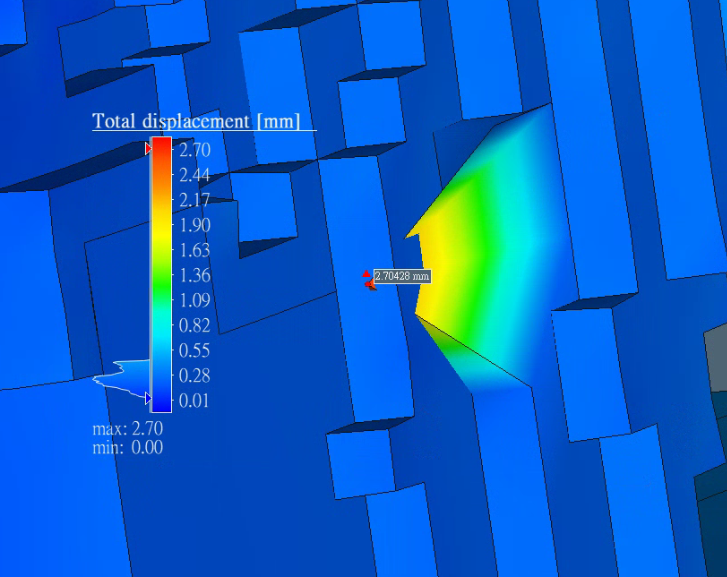
\includegraphics[width=0.6\textwidth]{images/bad_voxel.png}
  \caption{Screenshot of abnormal voxel behavior from simulation result. The voxel seems to be deformed and merging inside the structure itself. Luckily, only a handful of voxels of these sort exist, with the rest of the geometry showing much more sensible results.}
  \label{fig:bad_voxel}
\end{figure}

Table \ref{table:disp_bins} shows that there are some ranges of deformation that do not contain any nodes, meaning that there are discontinuities in the nodal deformations. This behavior is clearly non-physical, and suggests that these offending nodes should be discarded. To discard them, all nodes further away from three standard deviation were deleted from these topologies, and the statistics were recalculated. The graph of the maximum nodal displacements with corrected distributions are shown in Figure \ref{fig:disp_max_correct}. From this corrected figure it can be seen that there is local minima in the maximum nodal deformation for the results of the 40\% volume fraction simulations. Additionally, the differences between groups is much greater than the numerical uncertainty from the variation due to voxelization ( > 0.011 mm), making this result significant. Therefore, we can infer from this data that variation in topology does not result in a big effect on average node deformation, but can have an impact on the maximum node deformation of the resulting structure. 

\begin{table}[h!]
  \centering
  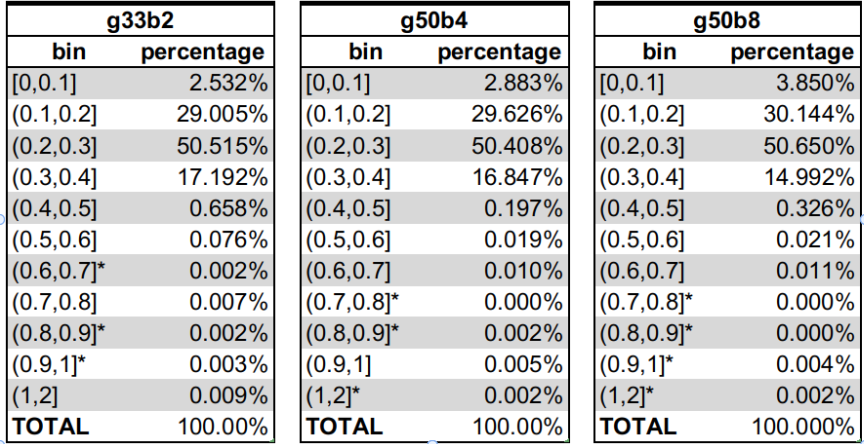
\includegraphics[width=0.75\textwidth]{images/results/plots/femoral/displacement/bins.png}
  \caption{Bins of nodal displacement for suspicious results. The bins labeled with an asterisk have very little to no members, indicating a discontinuous nodal deformation distribution. This is deemed to be non-physical and likely an error with the finite element result.}
  \label{table:disp_bins}
\end{table}

\begin{figure}[h!]
  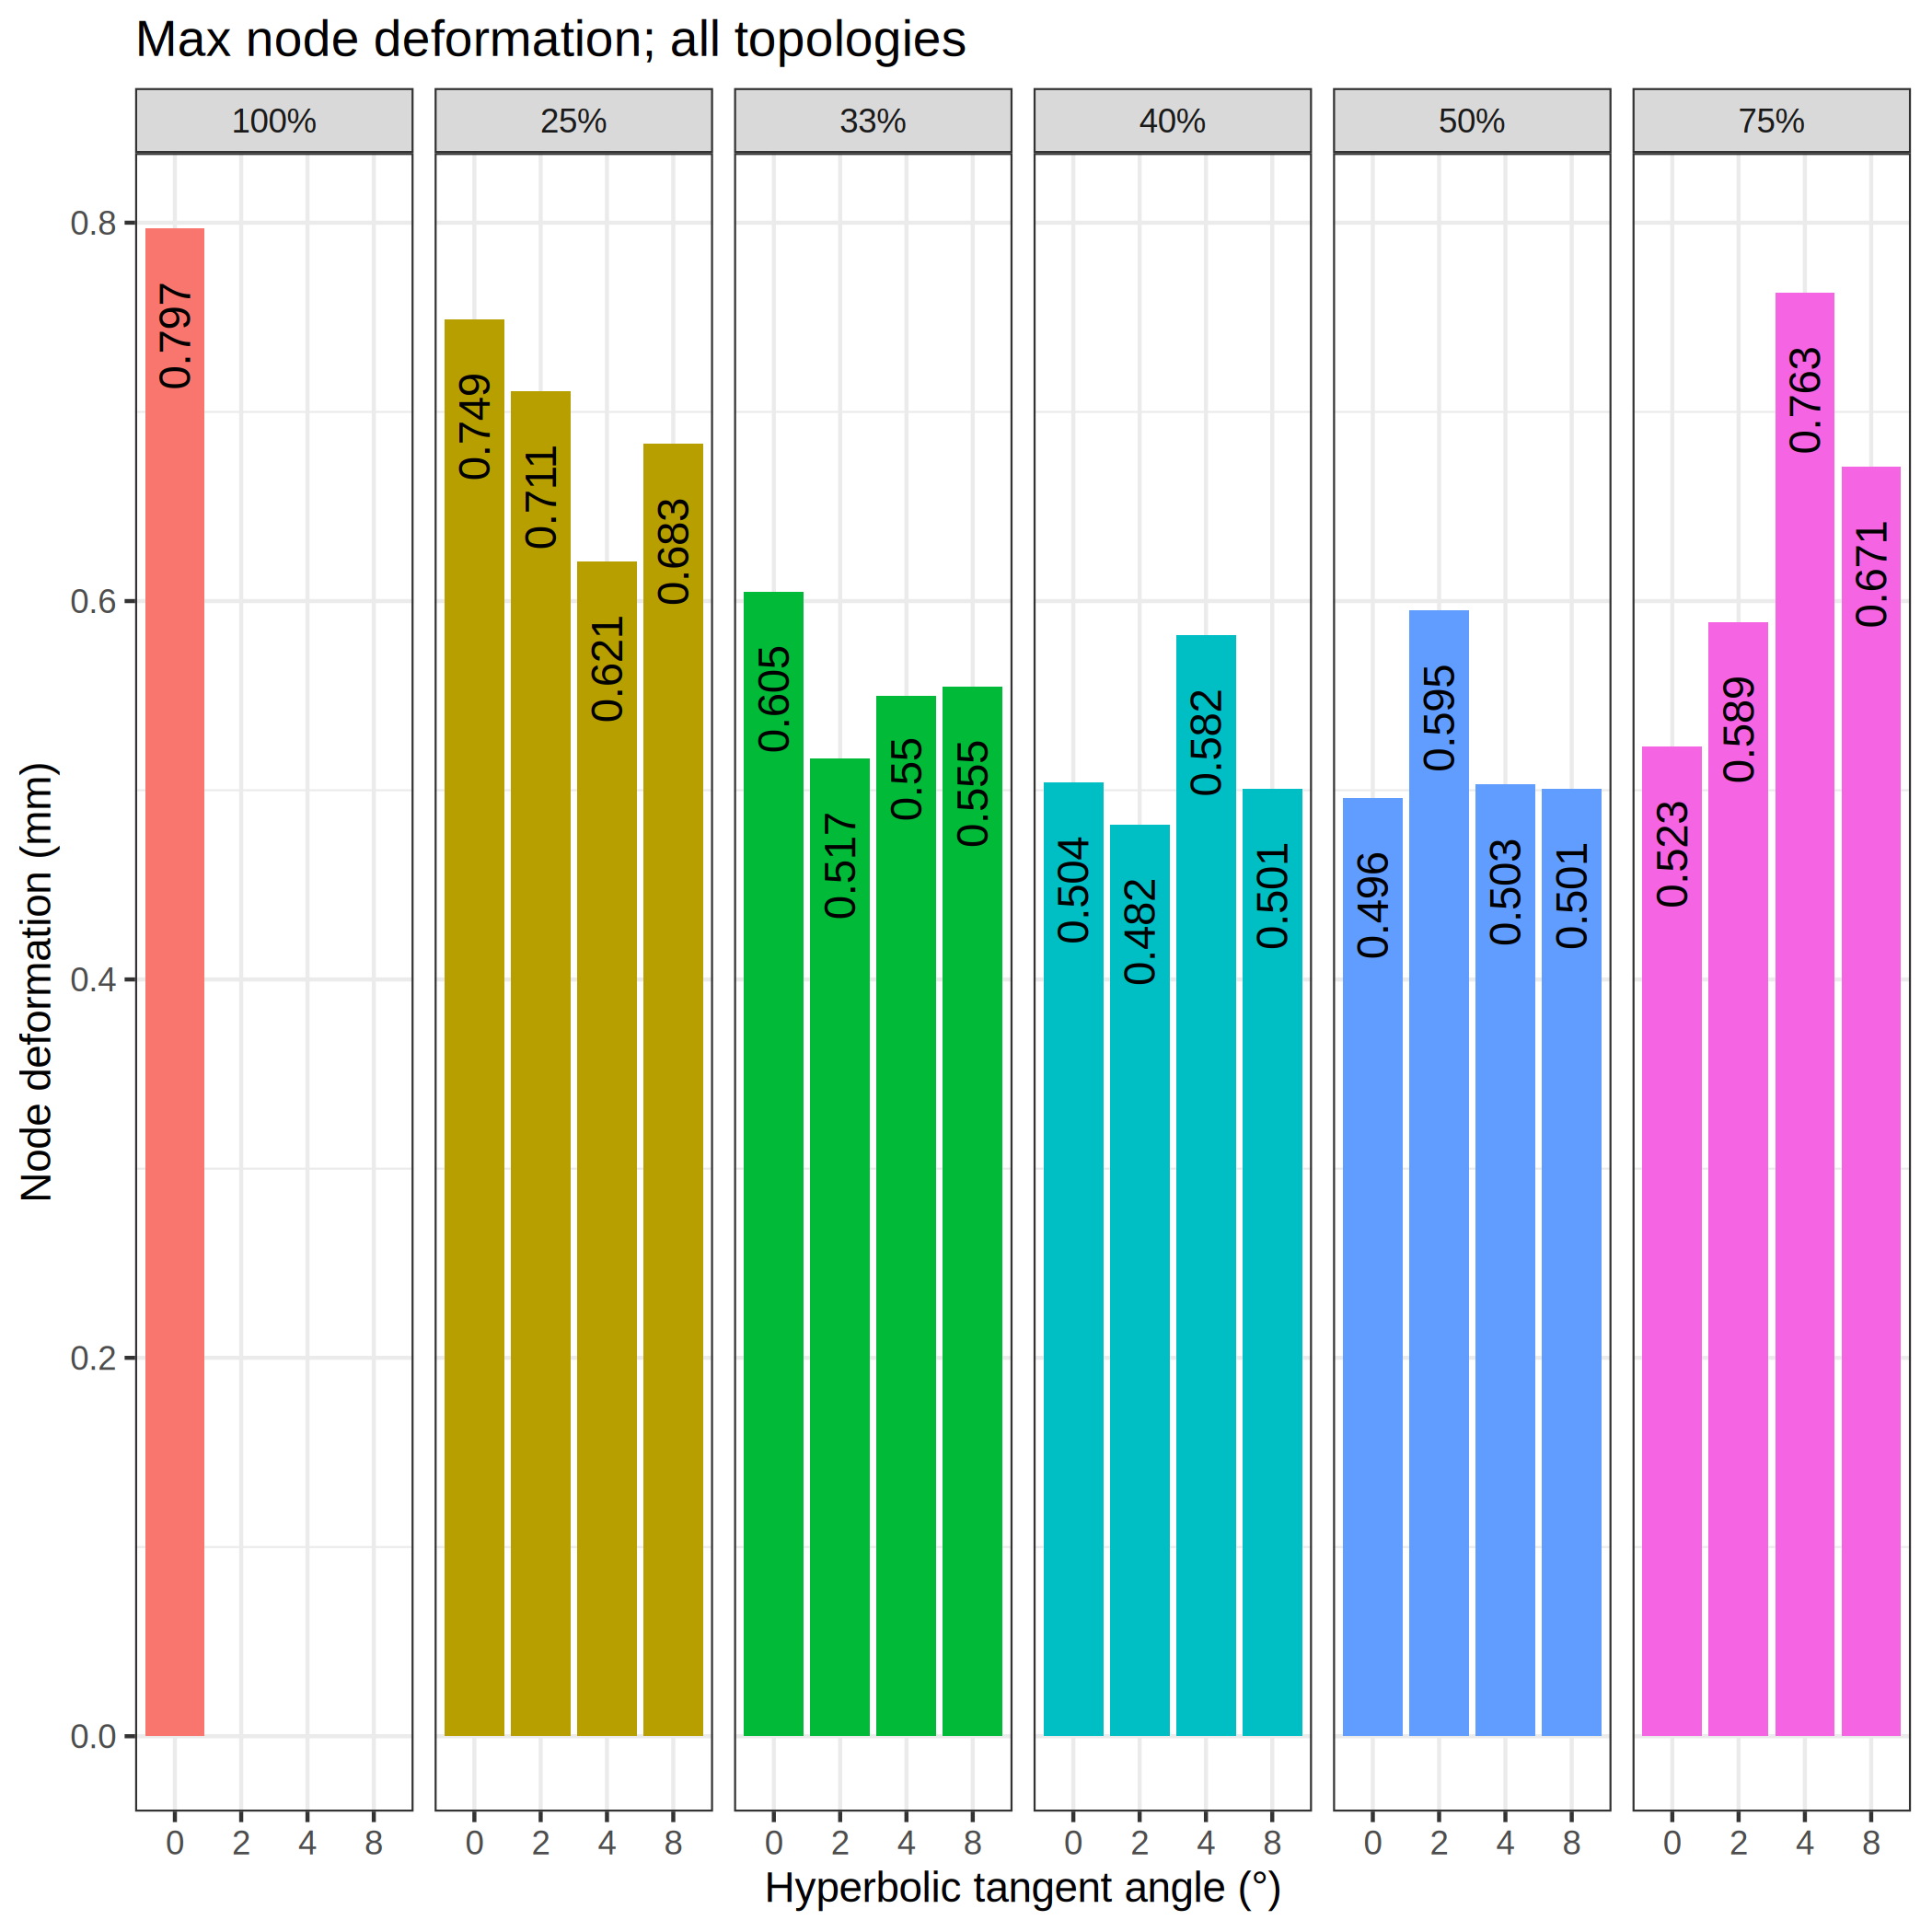
\includegraphics[width=0.45\textwidth]{images/results/plots/femoral/displacement/femoral_max.png}
  \hfill
  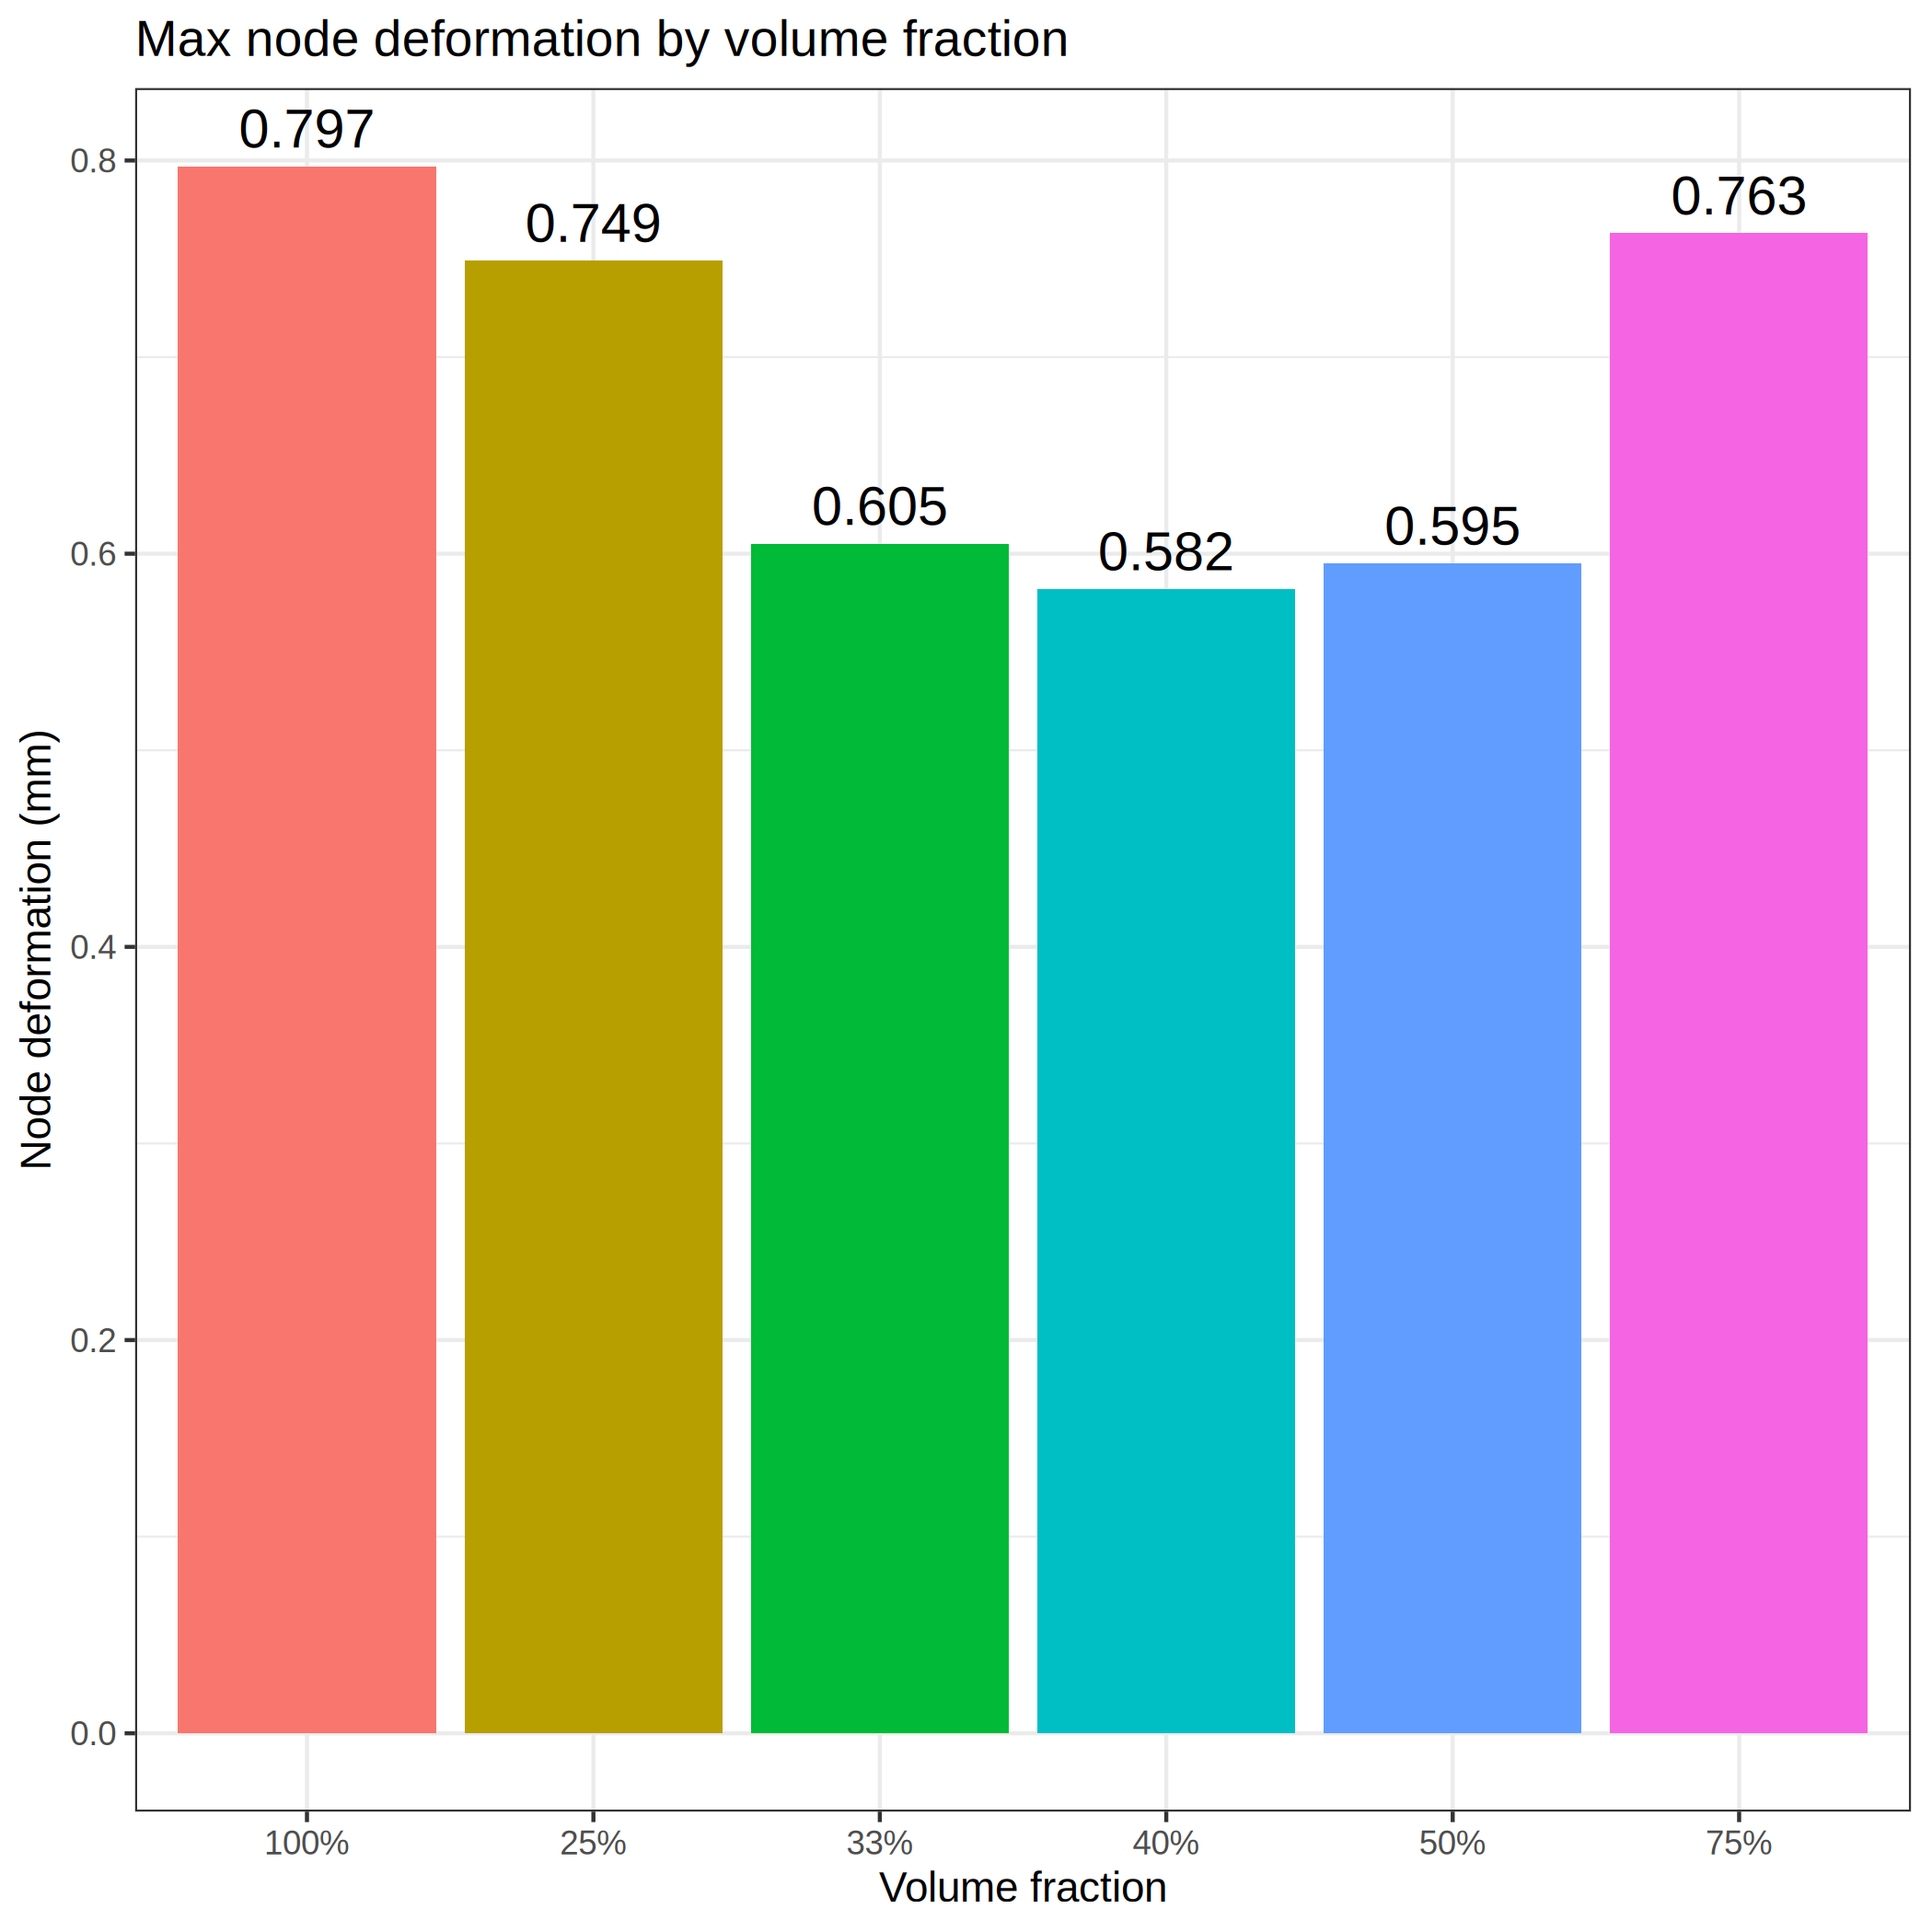
\includegraphics[width=0.45\textwidth]{images/results/plots/femoral/displacement/femoral_max_group.png}
  \caption{Maximum nodal displacement after corrections.}
  \label{fig:disp_max_correct}
\end{figure}

Lastly, all of the following trends can be succinctly visualized using a box and whisker plot, shown in Figure \ref{fig:disp_boxwhisker}. From this final plot we can see once more that the average deformation stays constant throughout, but that there is a local minimum in the maximum deformation in the groups with intermediate volume fractions. The full statistics of the nodal displacements are shown in Table \ref{table:disp_stats}.

Based on the node displacement analysis conducted for this support structure configuration, we have identified an optimal geometric arrangement characterized by a 40\% volume fraction and a hyperbolic tangent angle of 2 degrees. The empirical evidence demonstrates a non-linear relationship between structural performance and volume fraction, wherein both excessively high and low volume fractions correlate with elevated average node displacement values. This finding suggests that deformation minimization can be achieved through the implementation of intermediate volume fraction parameters. Additionally, just as the simple geometry study, the current displacement analysis is unable to find any strong relationship between hyperbolic angle and average or maximum node deformation. Nevertheless, it is still suggested to perform systematic variation of hyperbolic angle when designing support structures. The analysis reveals that even within groups of identical volume fractions, there are still specific angular values that yield optimal performance as measured by maximum node deformation.

\begin{figure}[h!]
  \centering
  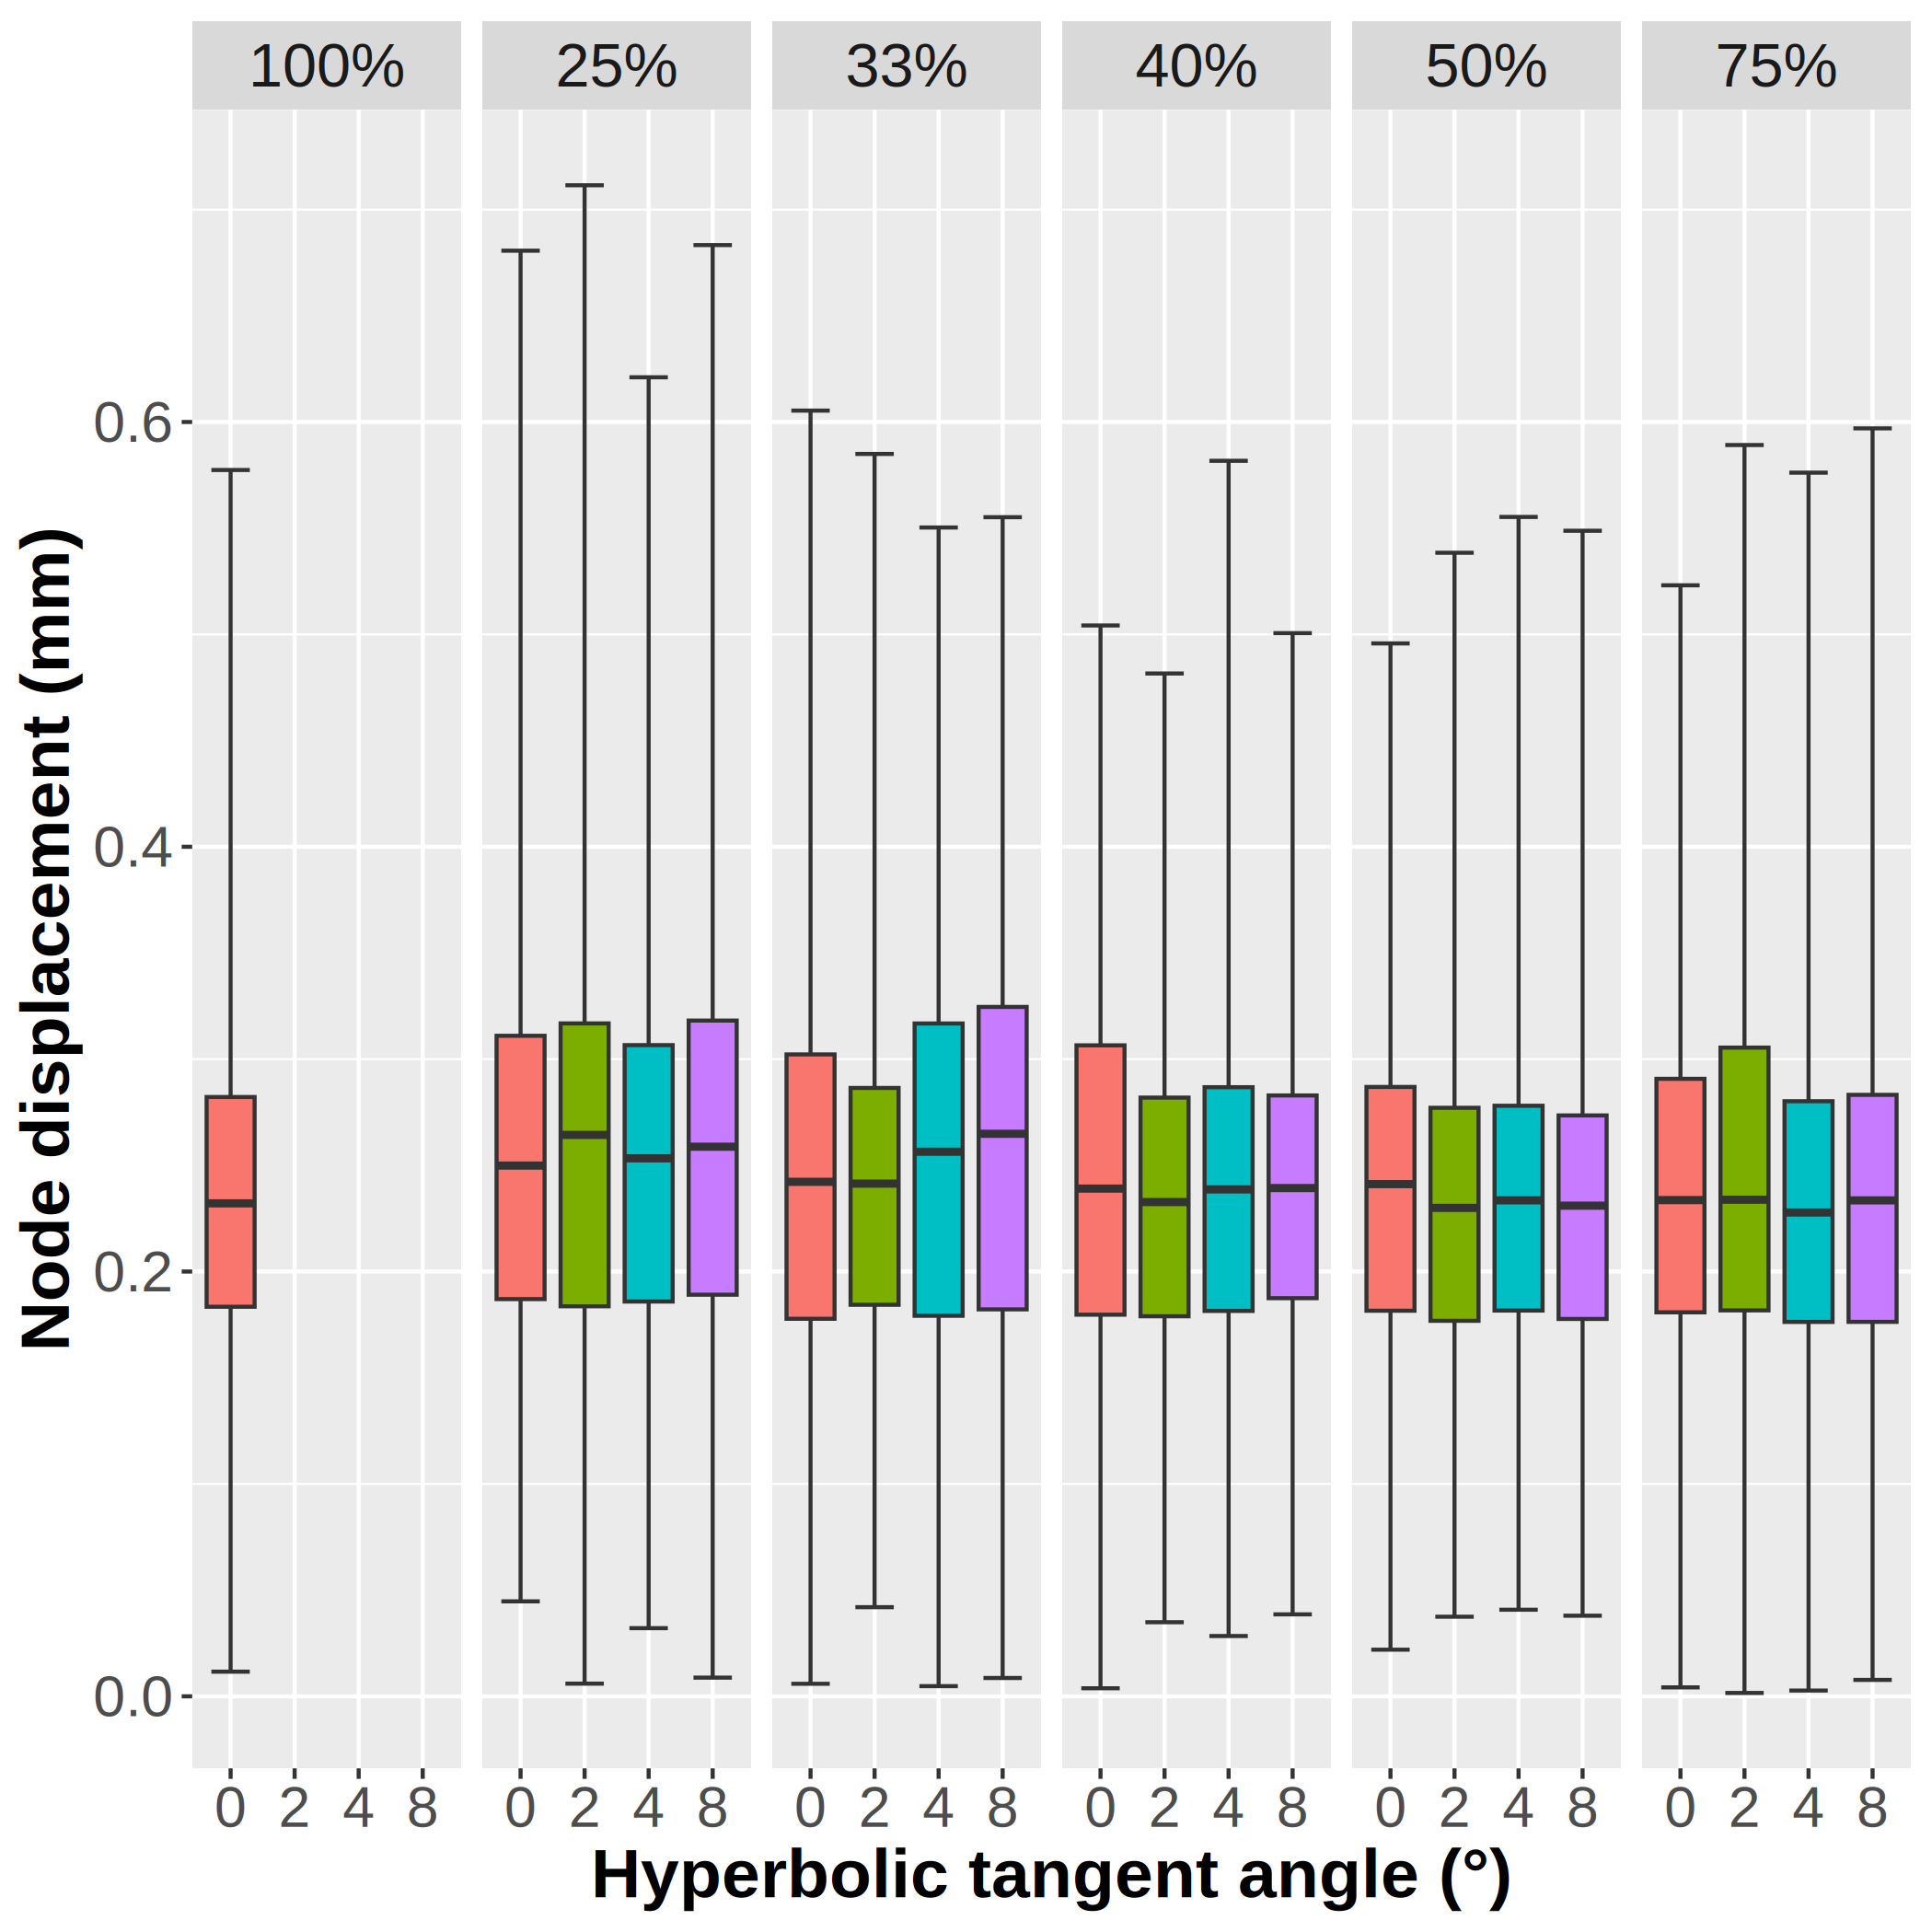
\includegraphics[width=0.6\textwidth]{images/results/plots/femoral/displacement/boxplots.png}
  \caption{Box and whisker plot for femoral displacement of all topologies.}
  \label{fig:disp_boxwhisker}
\end{figure}

\begin{table}[h!]
  \centering 
  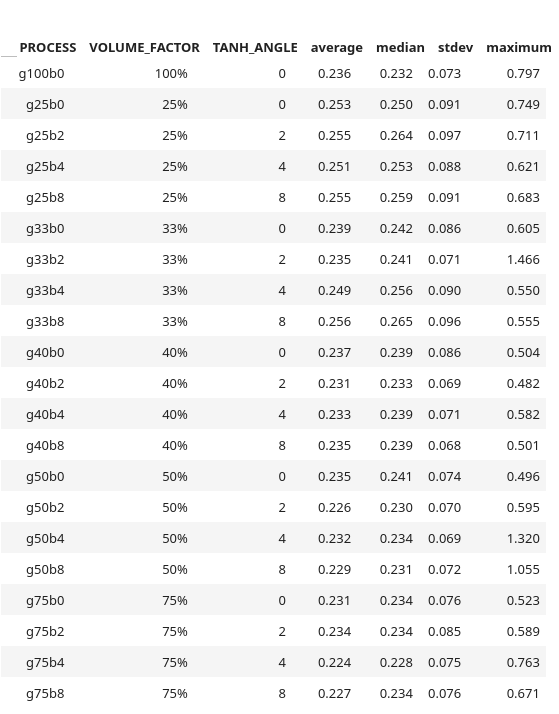
\includegraphics[width=0.8\textwidth]{images/results/plots/femoral/displacement/statistics.png}
  \caption{Statistics of nodal displacements (mm); all topologies}
  \label{table:disp_stats}
\end{table}

\clearpage
\subsection{Stress analysis}

To analyze the differences in internal stresses caused by the topologies, we inspect the node stress density distributions. In contrast with the displacement density distribution, there is very little variability between groups. On the other hand, across groups we can see differences in the spread of stress. For example, the stress are most densely concentrated around the peak of the 25\% group compared to the groups with higher volume fractions, such as 50\% and 75\%. This indicates that some groups have smaller standard deviations, with values more closely packed together. This can be confirmed by looking at the statistics in  
Table \ref{table:stress_stats}, where we can see slight differences in the standard deviation of topologies.

Next, we inspect the average displacement of the simulation results. We can see that the baseline case has the smallest average stresses, but as soon as topologies with lower volume fraction are used, the average stresses rises more than 20\%, from a baseline value of 400 MPa to over 485 MPa. The average stress does not change considerably from topology to topology, which is similar to what was noticed for the average nodal displacement. This trend is shown in Figure \ref{fig:average_stresses}. Looking at the maximum stress yields a very interesting result; namely, that all of the topologies have a near constant maximum stress. This result is clear from looking at both graphs in Figure \ref{fig:maximum_stresses}.

Lastly, the box-whisker plot of Figure \ref{fig:stress_boxwhisker} shows a succinct summary of all the statistics discussed in this section.

The stress analysis results was not able to reveal any correlations between both volume fraction and nodal stress, as well as between hyperbolic tangent angle and nodal stress. This is an anomalous finding, given that all simulations produced remarkably consistent maximum stress values with minimal variations in standard deviation and average nodal stresses across configurations. The homogeneity of stress results across all the different supporting structure geometries might be an indication of methodological issues in the simulation approach or computational limitations in the finite element software. These suspiciously uniform outcomes warrant further investigation.  

A more comprehensive stress analysis approach would involve examining the spatial distribution and concentration of stresses throughout the entire three-dimensional structure, rather than relying solely on statistical measures of nodal stress. By generating detailed stress field maps, researchers could identify critical high-stress regions, stress gradients, and potential failure initiation points within the support structure. This methodology would provide more meaningful insights into the structural behavior and better illuminate the relationships between geometric parameters (volume fraction and hyperbolic tangent angle) and mechanical performance. Such visualization-based analysis would likely reveal patterns and correlations that were obscured by the aggregate statistical approach, thereby offering more valuable guidance for future support structure optimization.


\begin{figure}[h!]
  \centering
  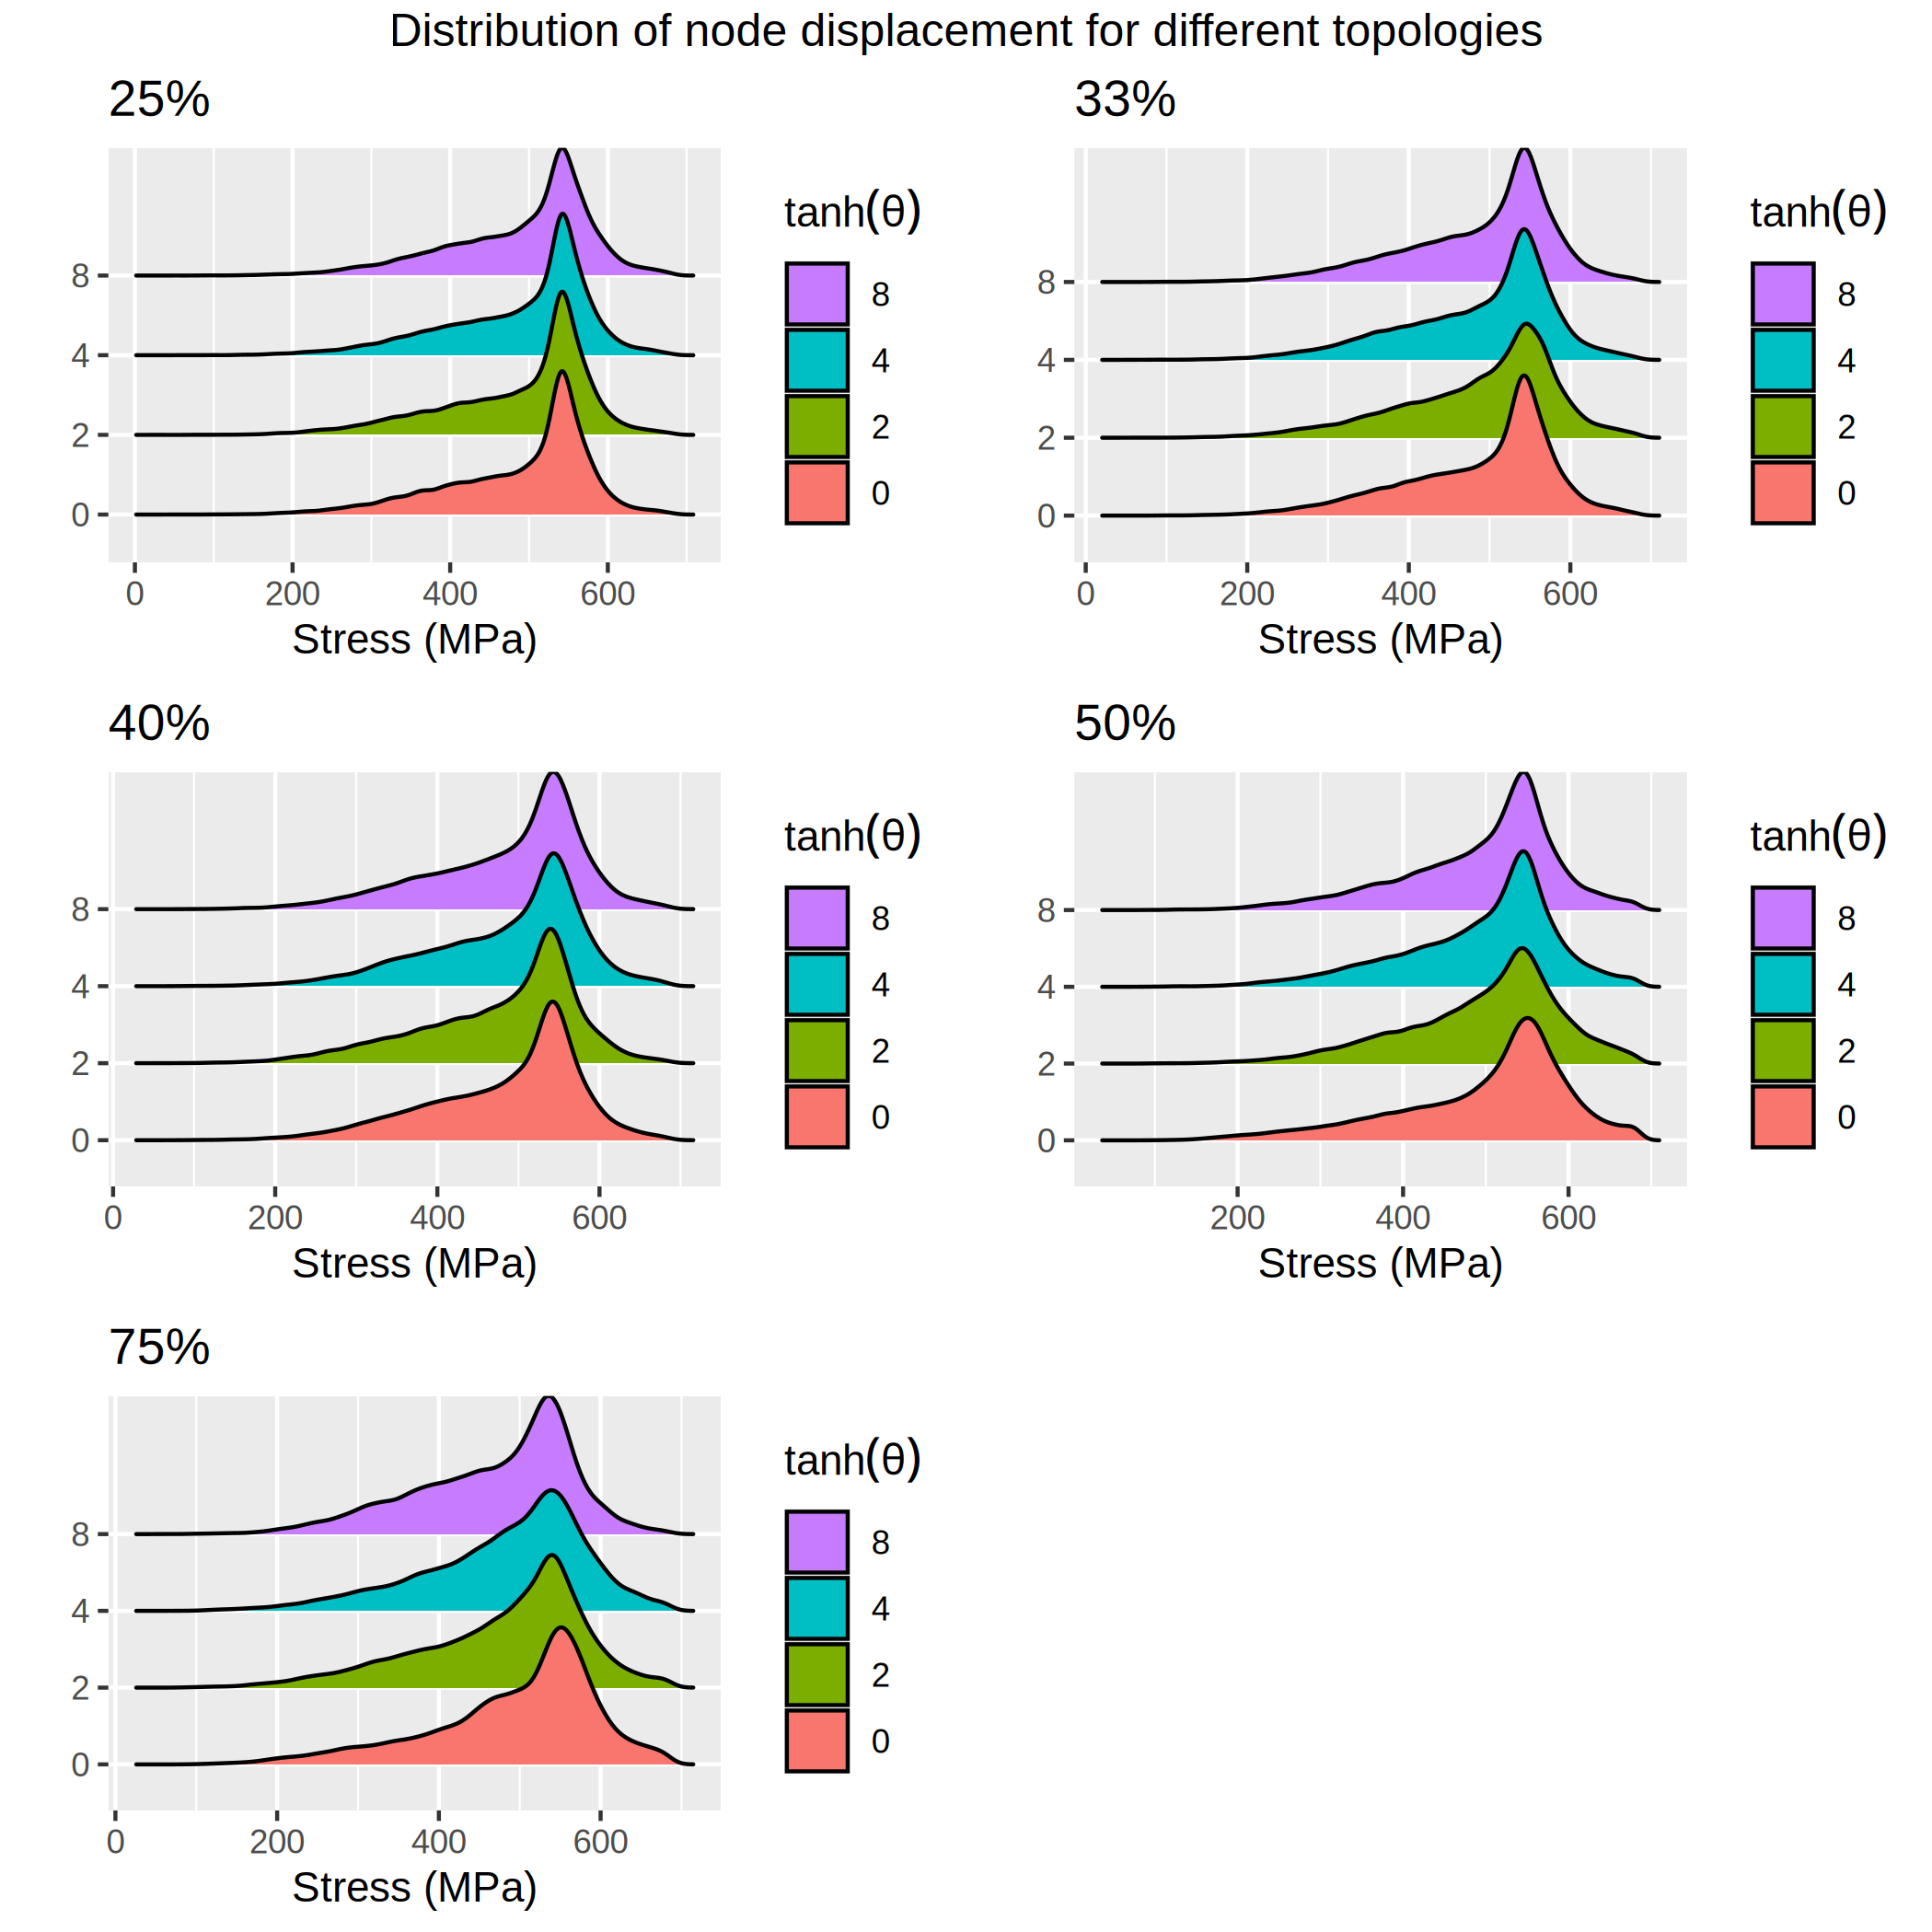
\includegraphics[width=0.75\textwidth]{images/results/plots/femoral/stress/stress_density_ridges.png}
  \caption{Distribution of node stresses of support structures for femoral component.}
\end{figure}

\begin{table}[h!]
  \centering
  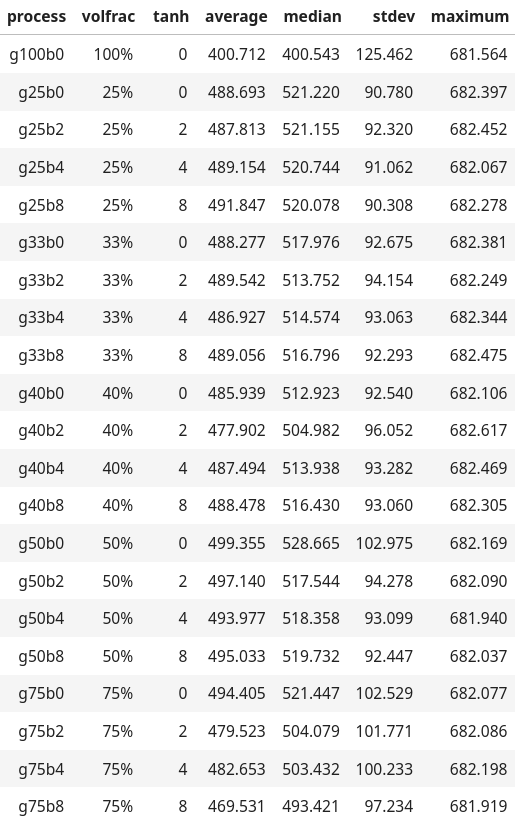
\includegraphics[width=0.75\textwidth]{images/results/plots/femoral/stress/stress_stats.png}
  \caption{Statistics of nodal stresses (MPa); all topologies.}
  \label{table:stress_stats}
\end{table}

\begin{figure}[h!]
  \centering
  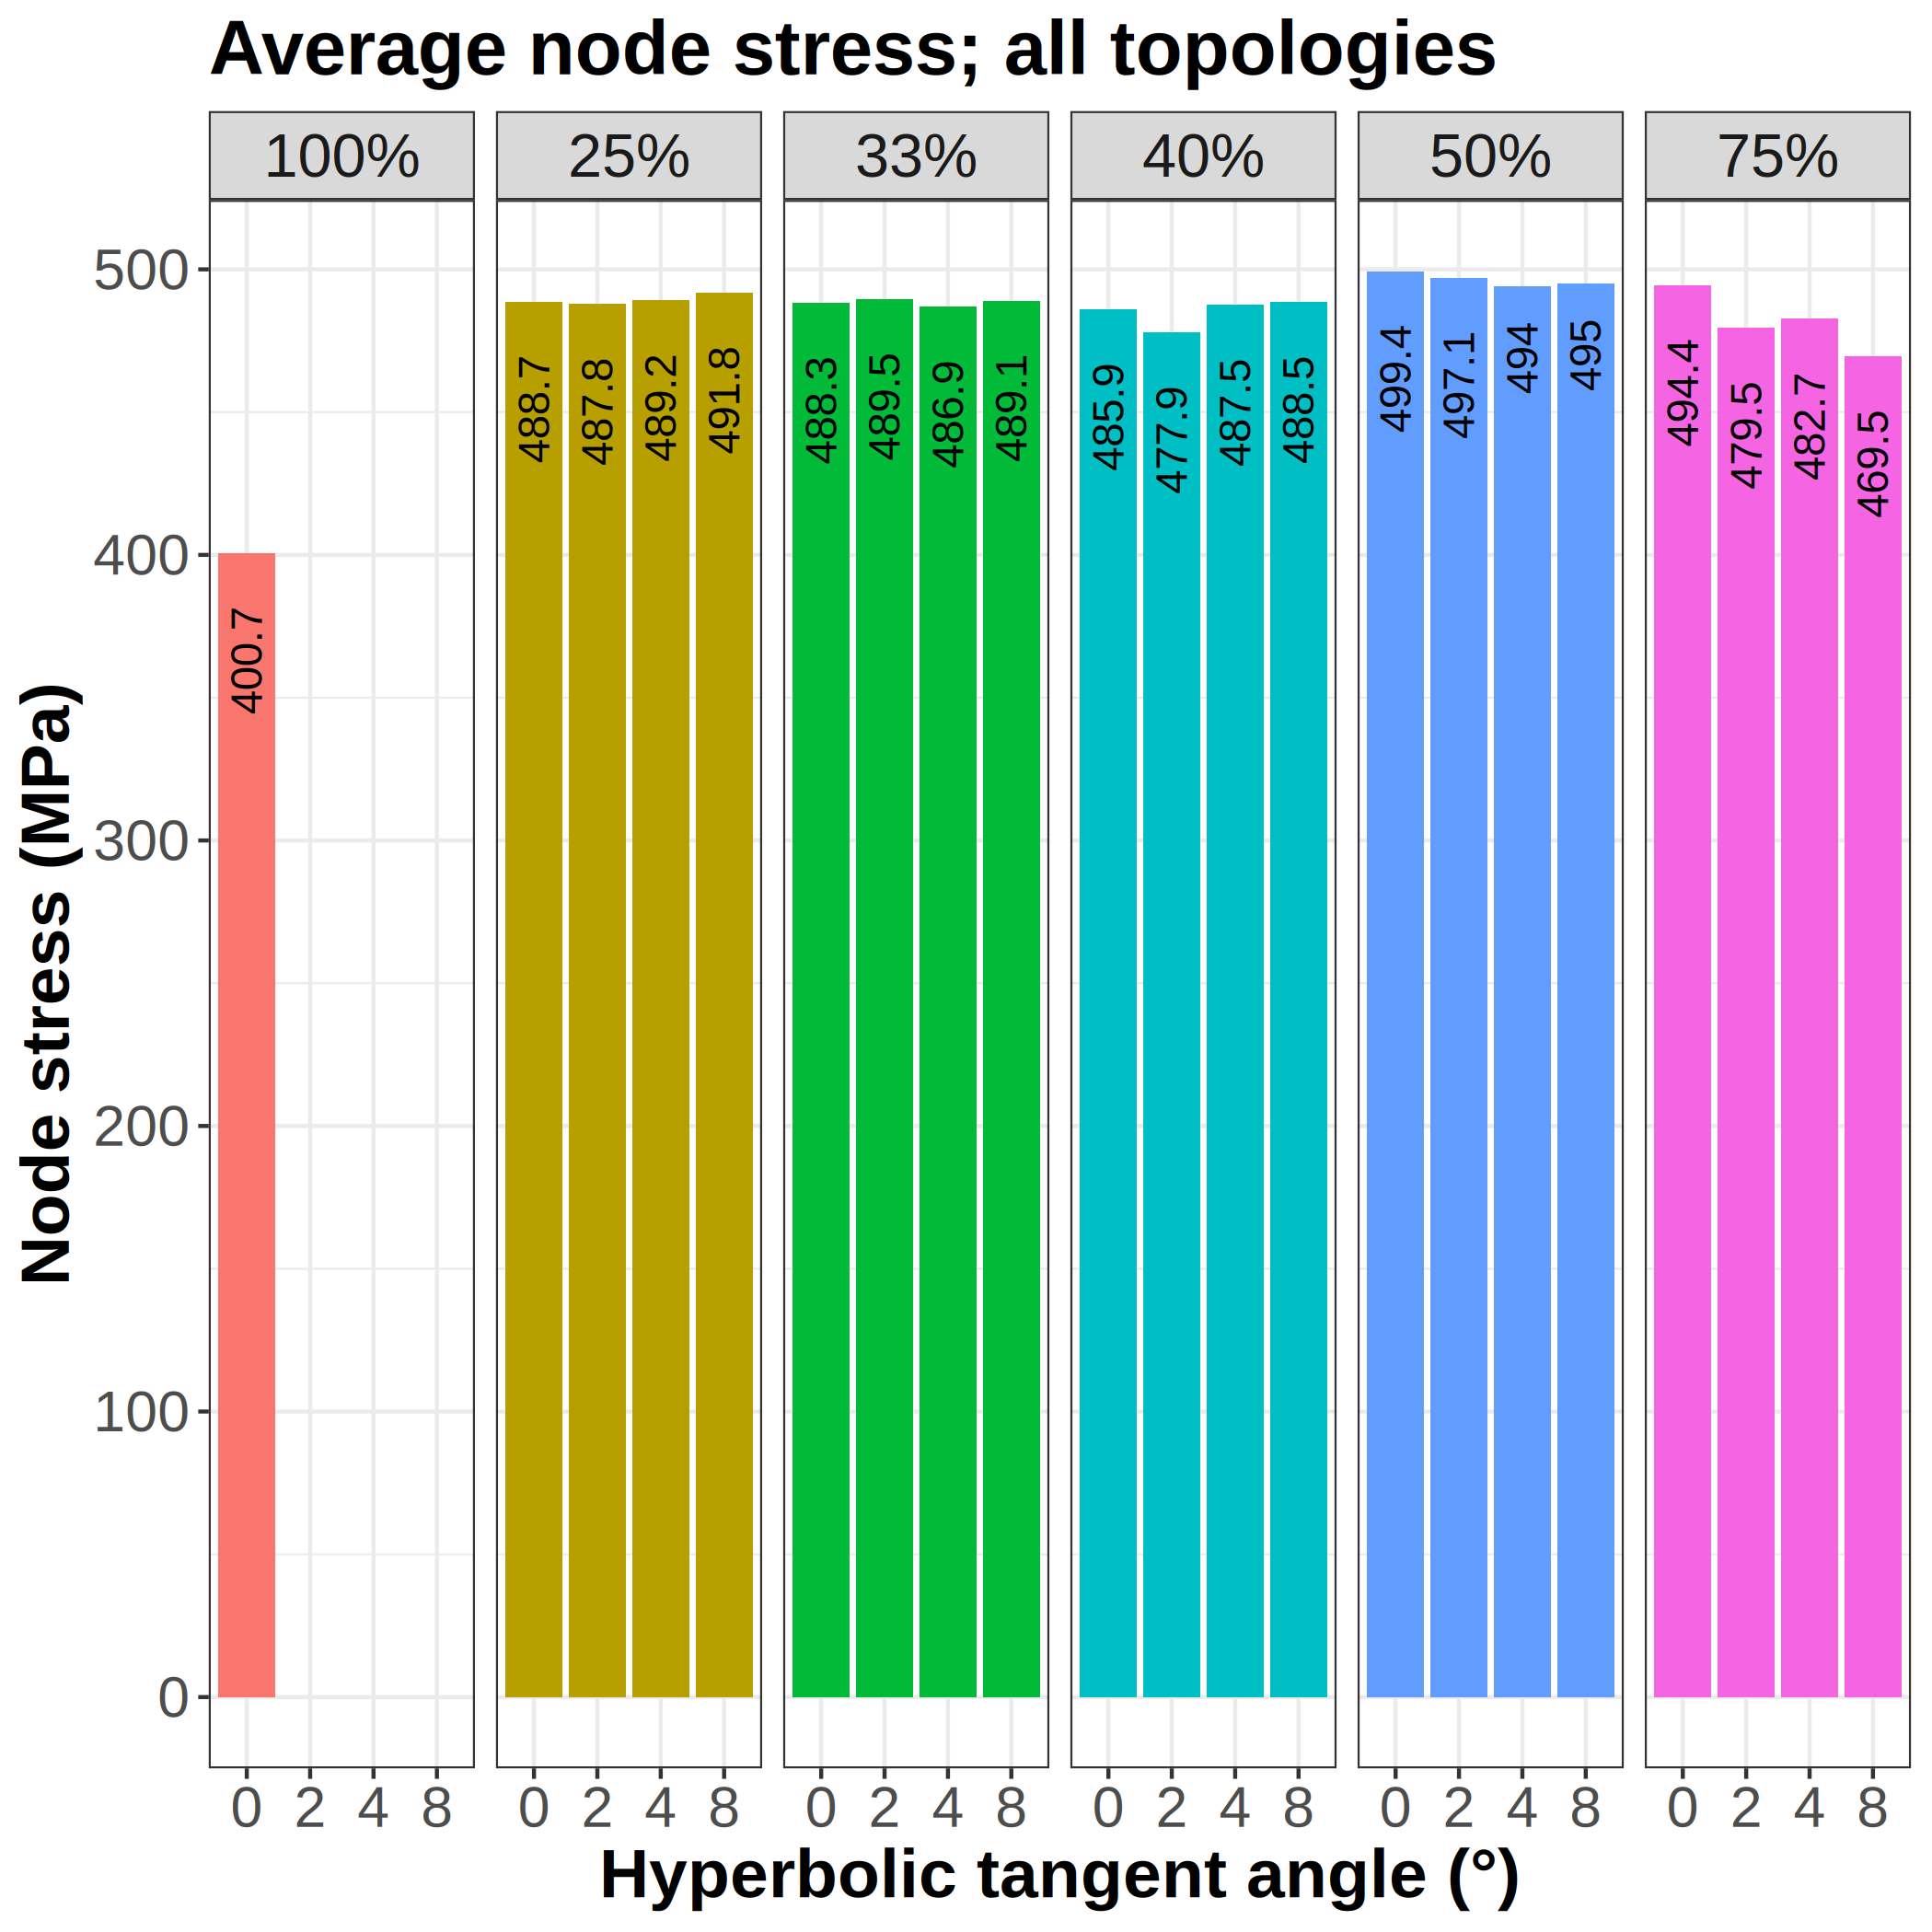
\includegraphics[width=0.45\textwidth]{images/results/plots/femoral/stress/average_stress.png}
  \hfill
  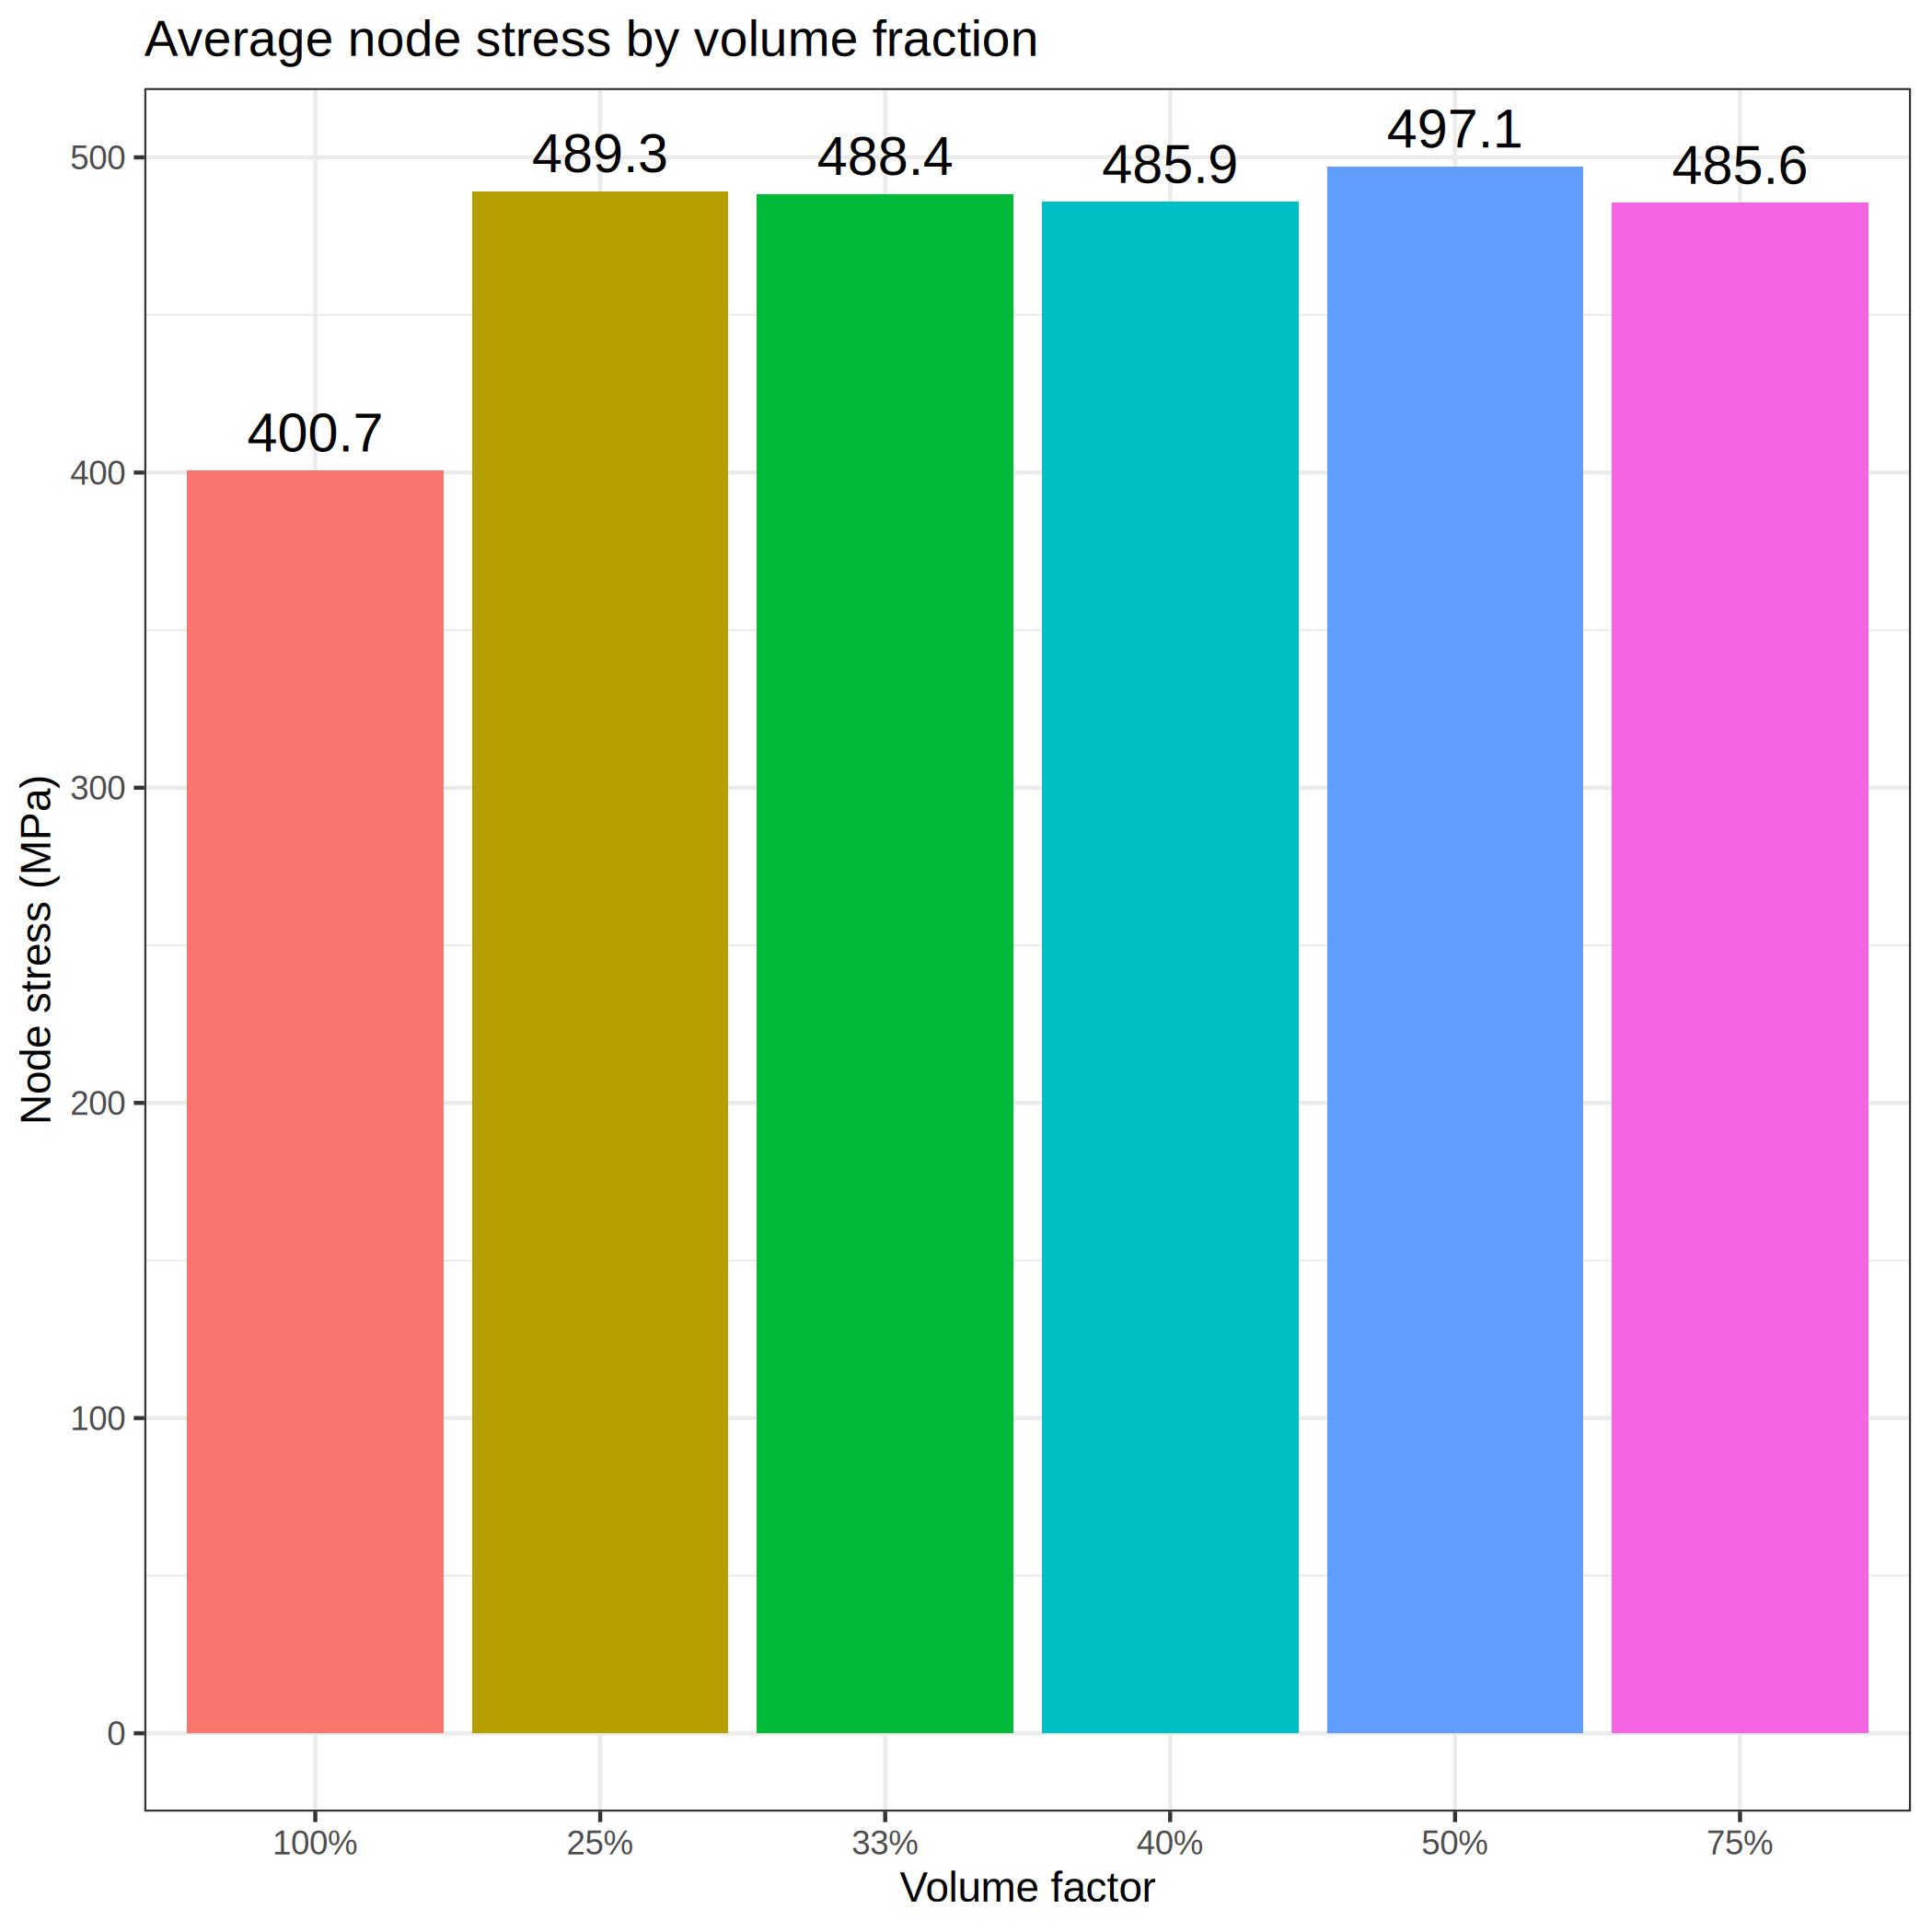
\includegraphics[width=0.45\textwidth]{images/results/plots/femoral/stress/femoral_average_group_stress.png}
  \caption{Average node stress for supporting structure of femoral component.}
  \label{fig:average_stresses}
\end{figure}

\begin{figure}[h!]
  \centering
  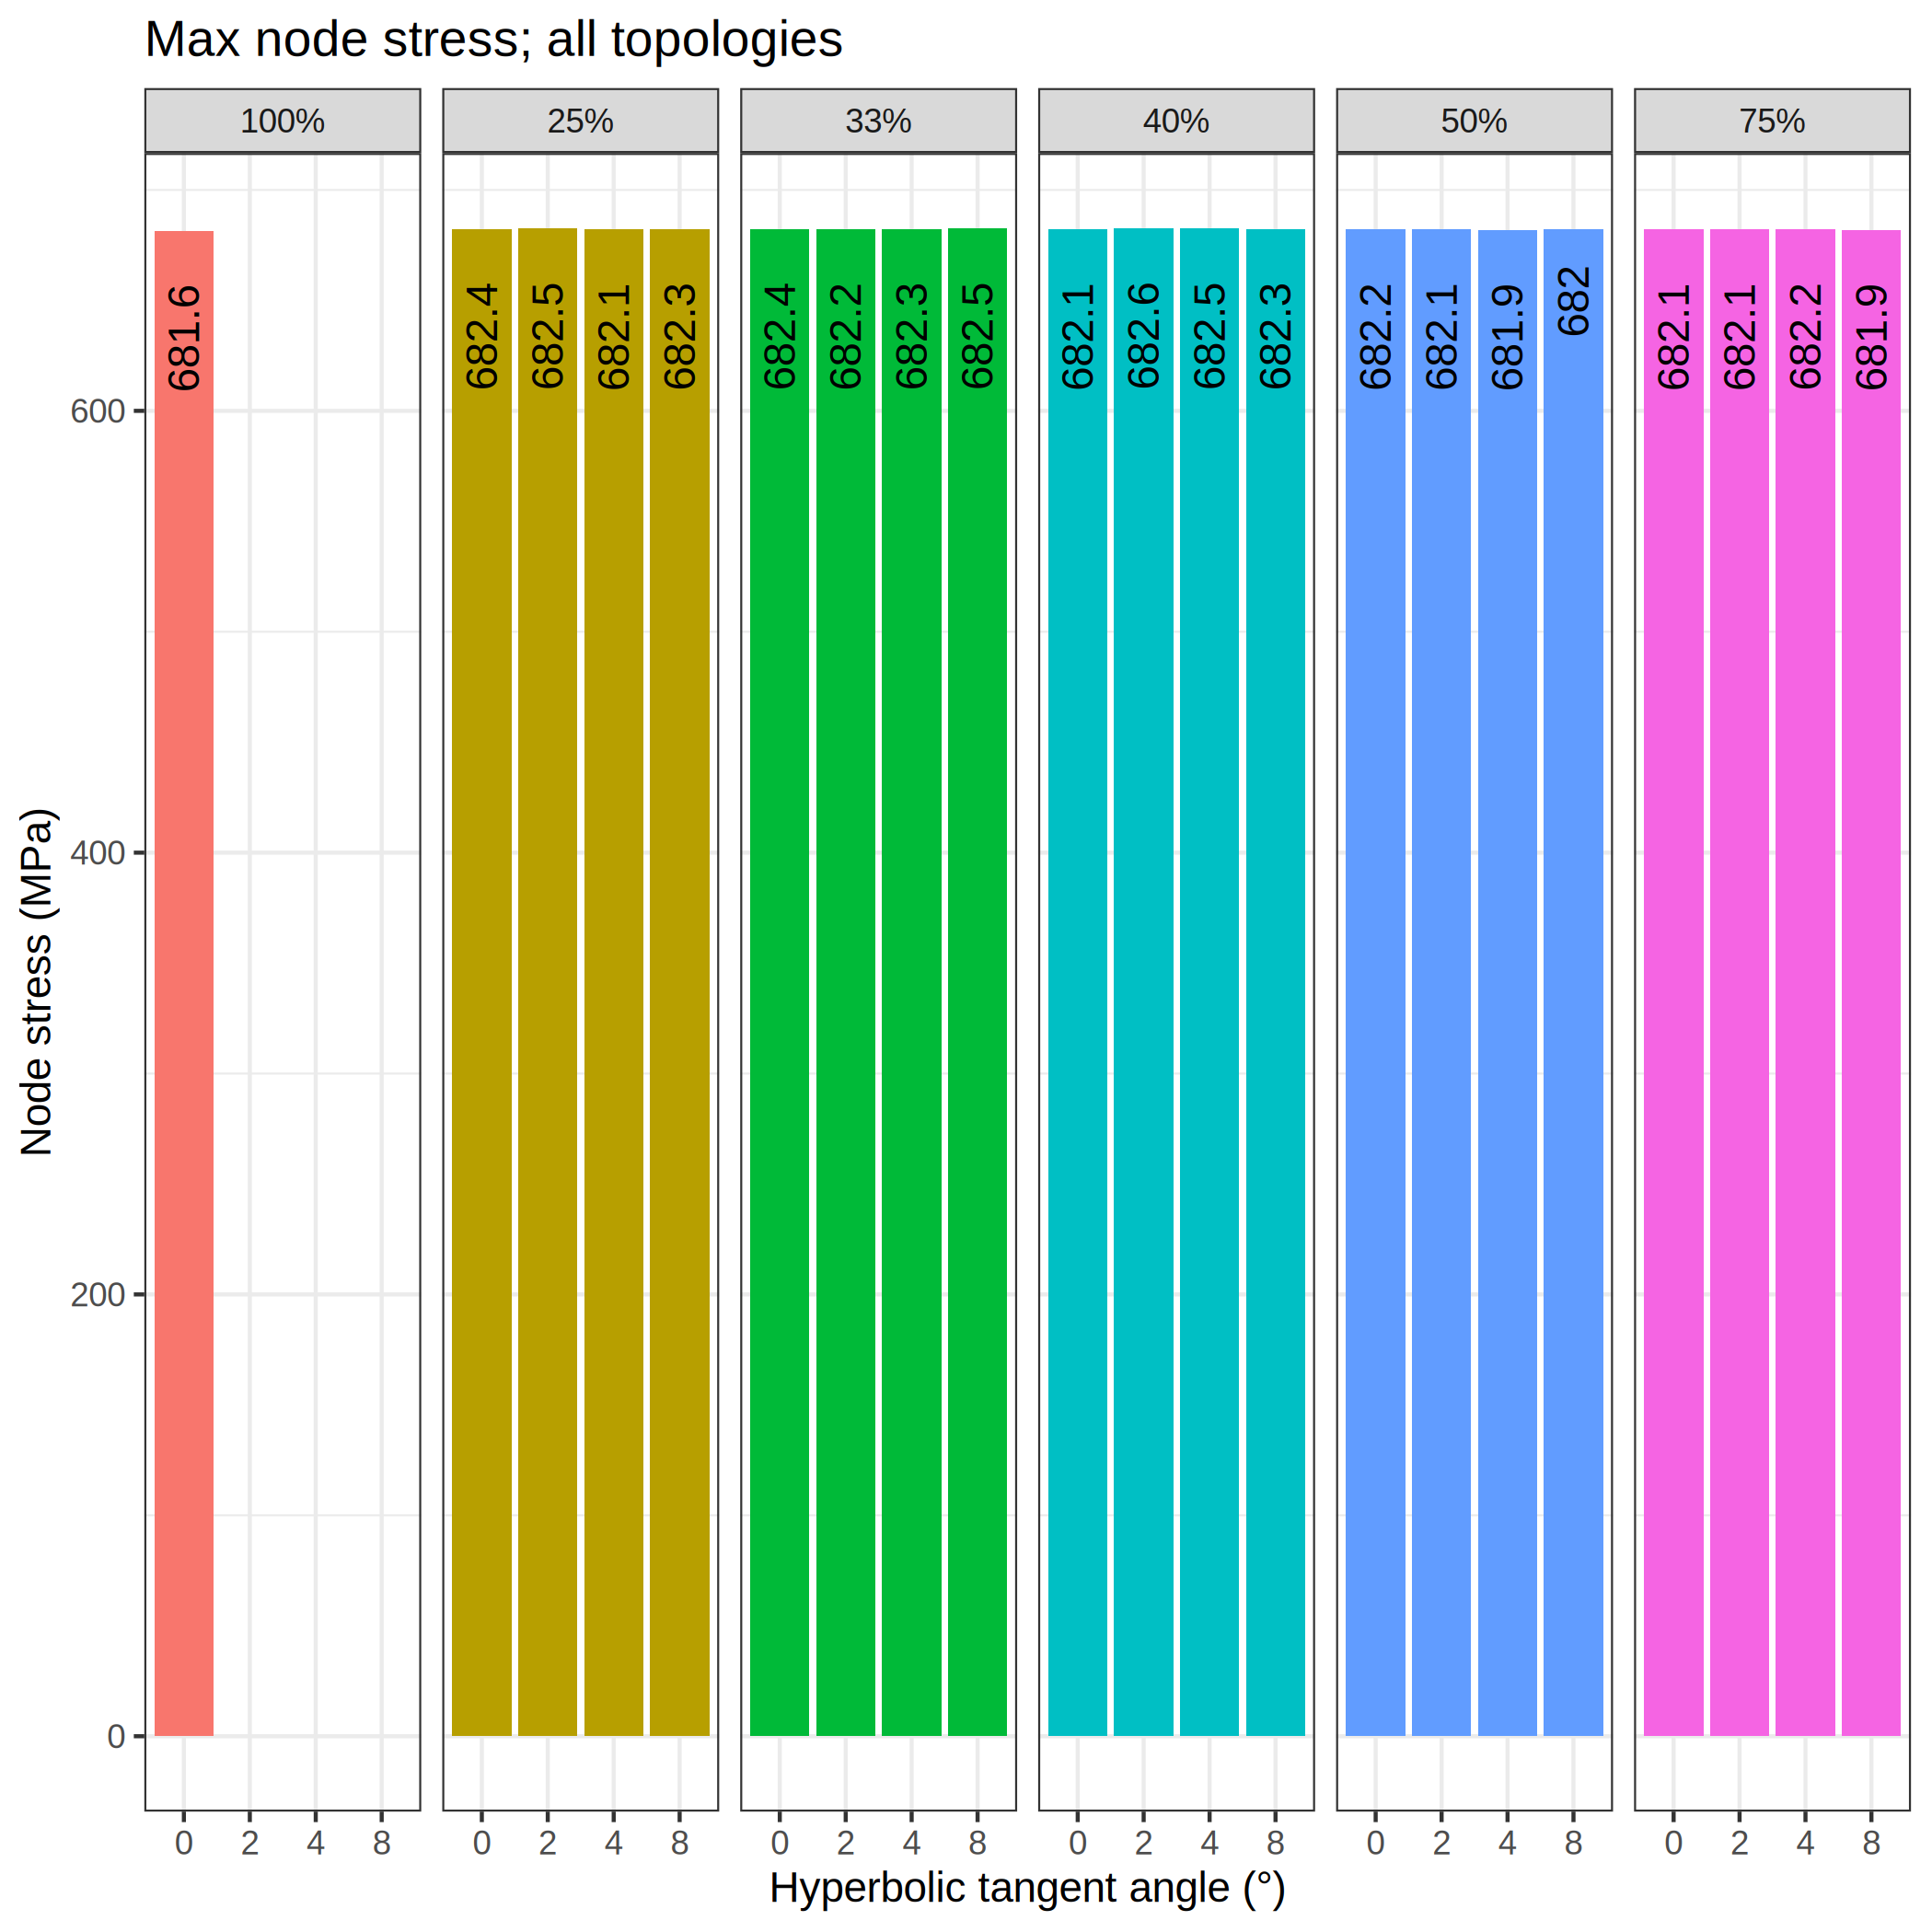
\includegraphics[width=0.45\textwidth]{images/results/plots/femoral/stress/maximum_stress.png}
  \hfill
  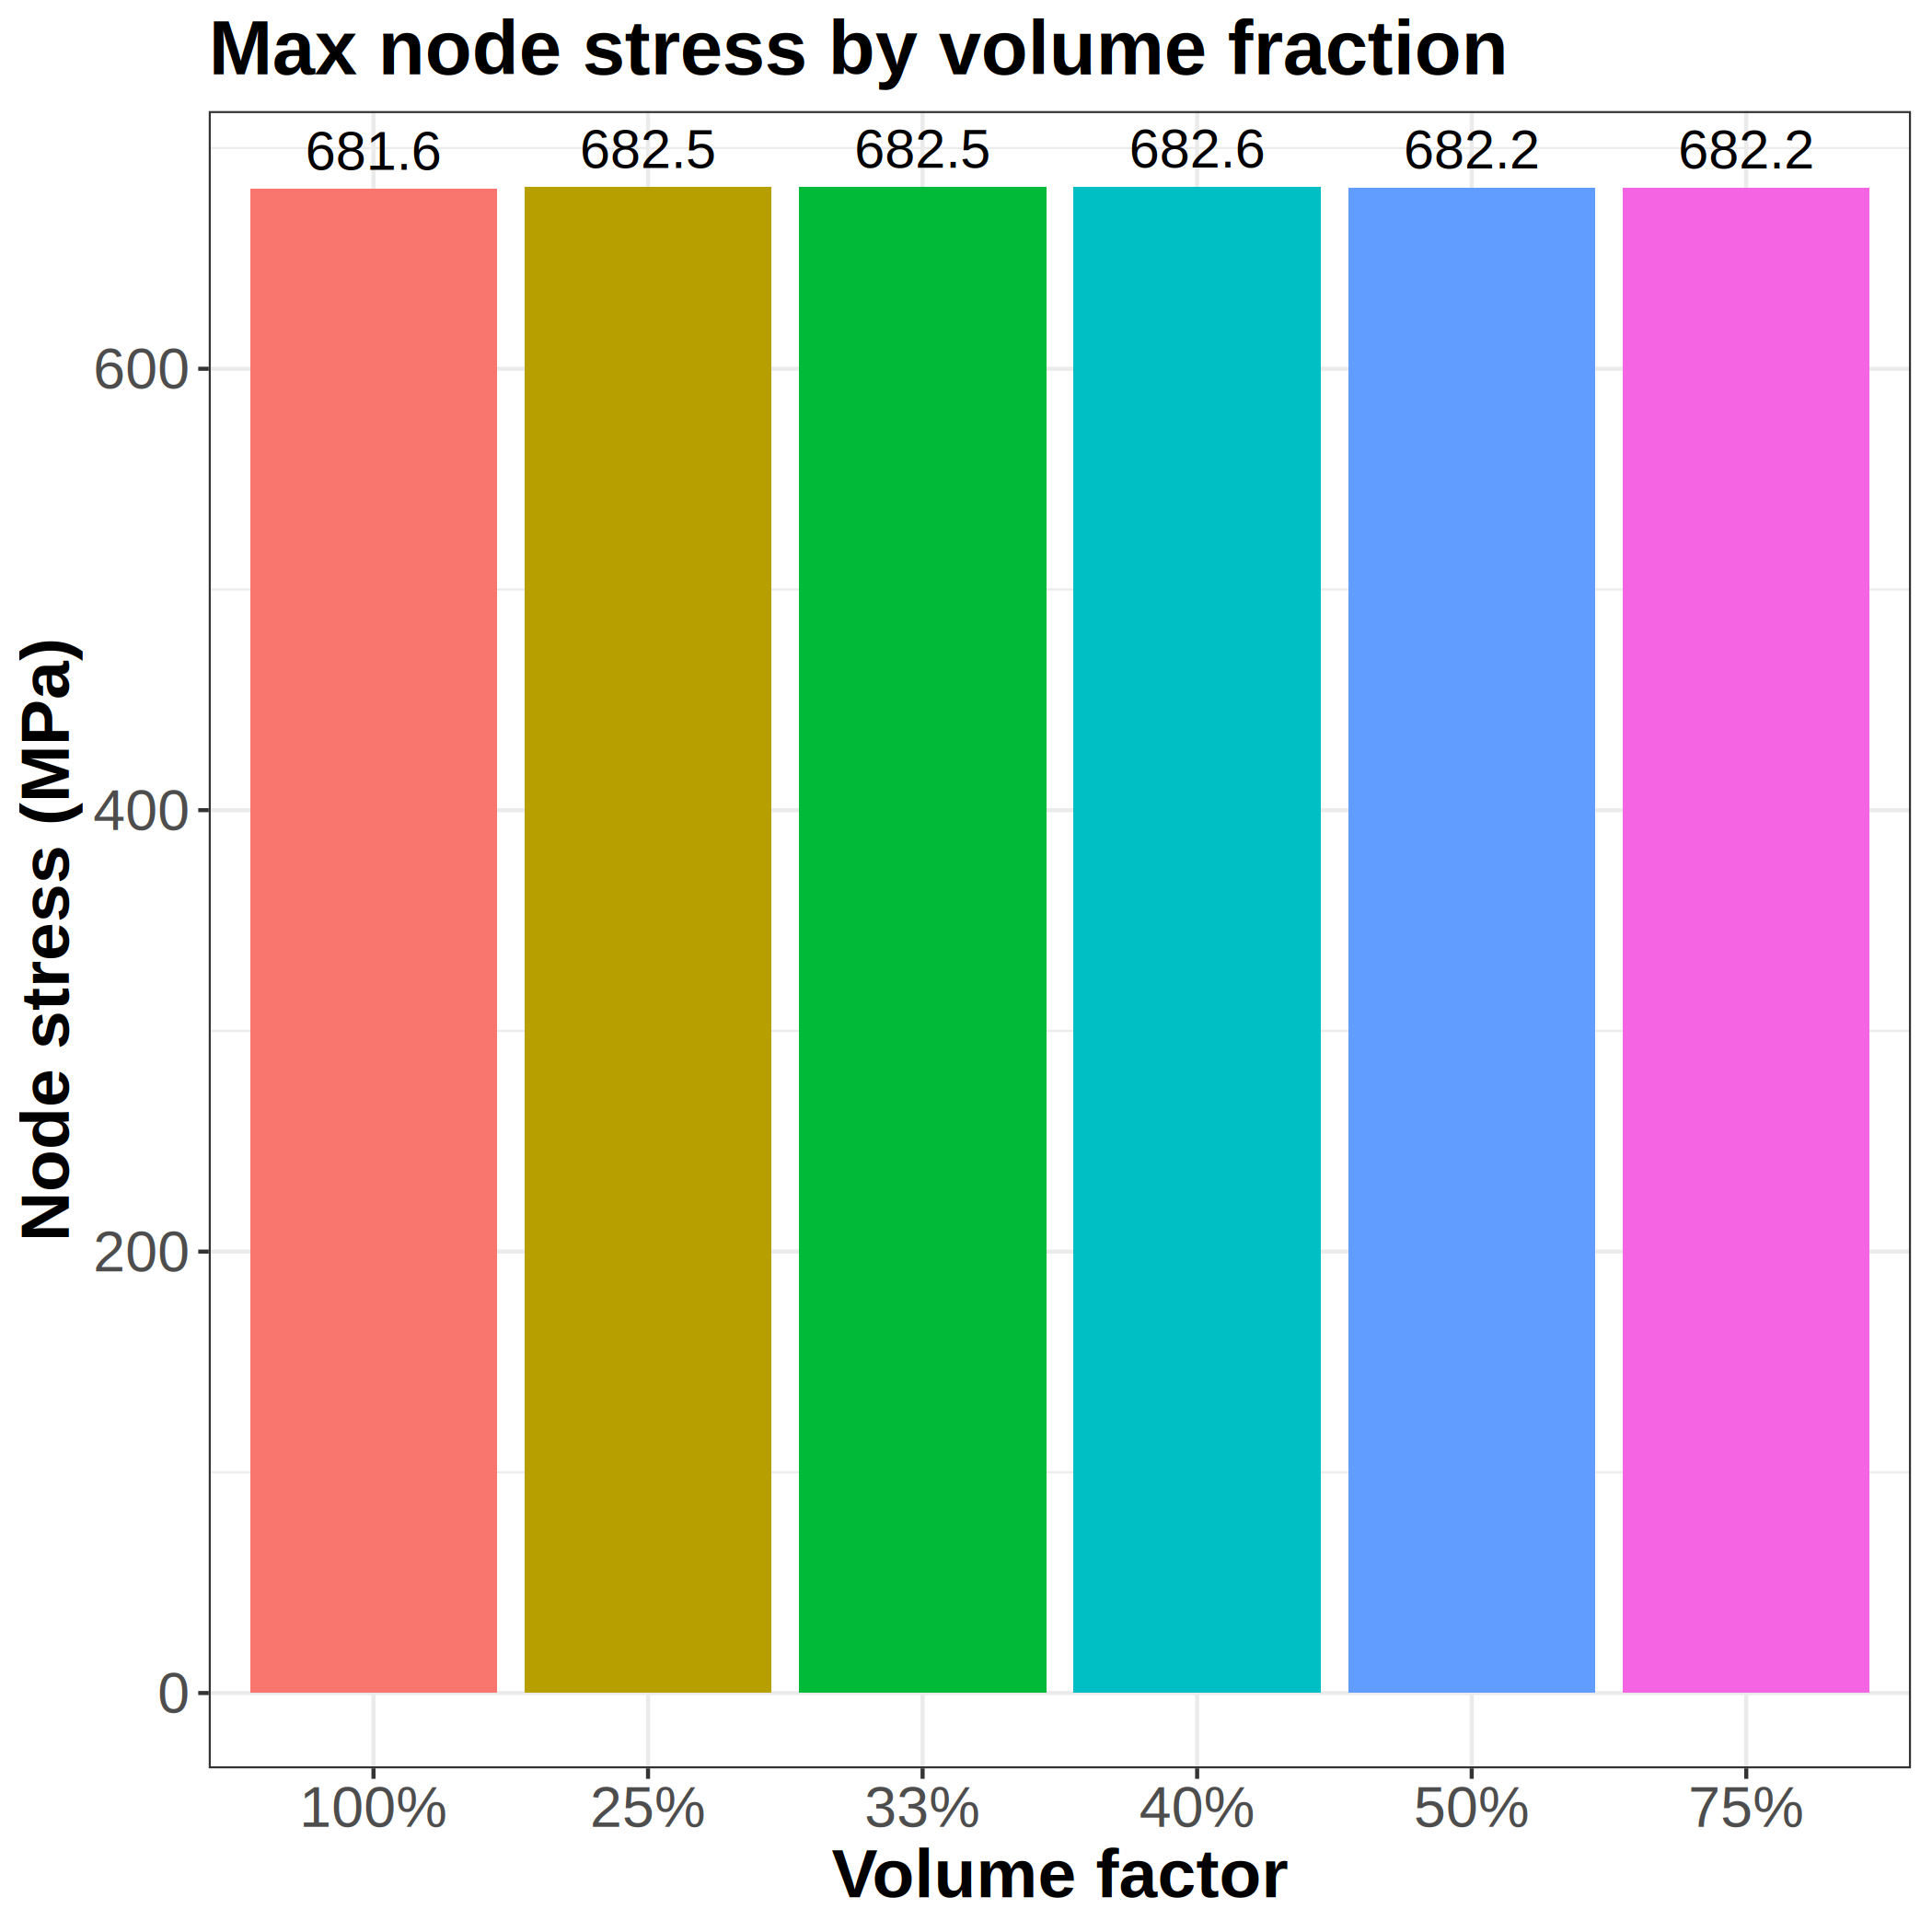
\includegraphics[width=0.45\textwidth]{images/results/plots/femoral/stress/femoral_max_group_stress.png}
  \caption{Maximum node stress for supporting structure of femoral component.}
  \label{fig:maximum_stresses}
\end{figure}

\begin{figure}[h!]
  \centering
  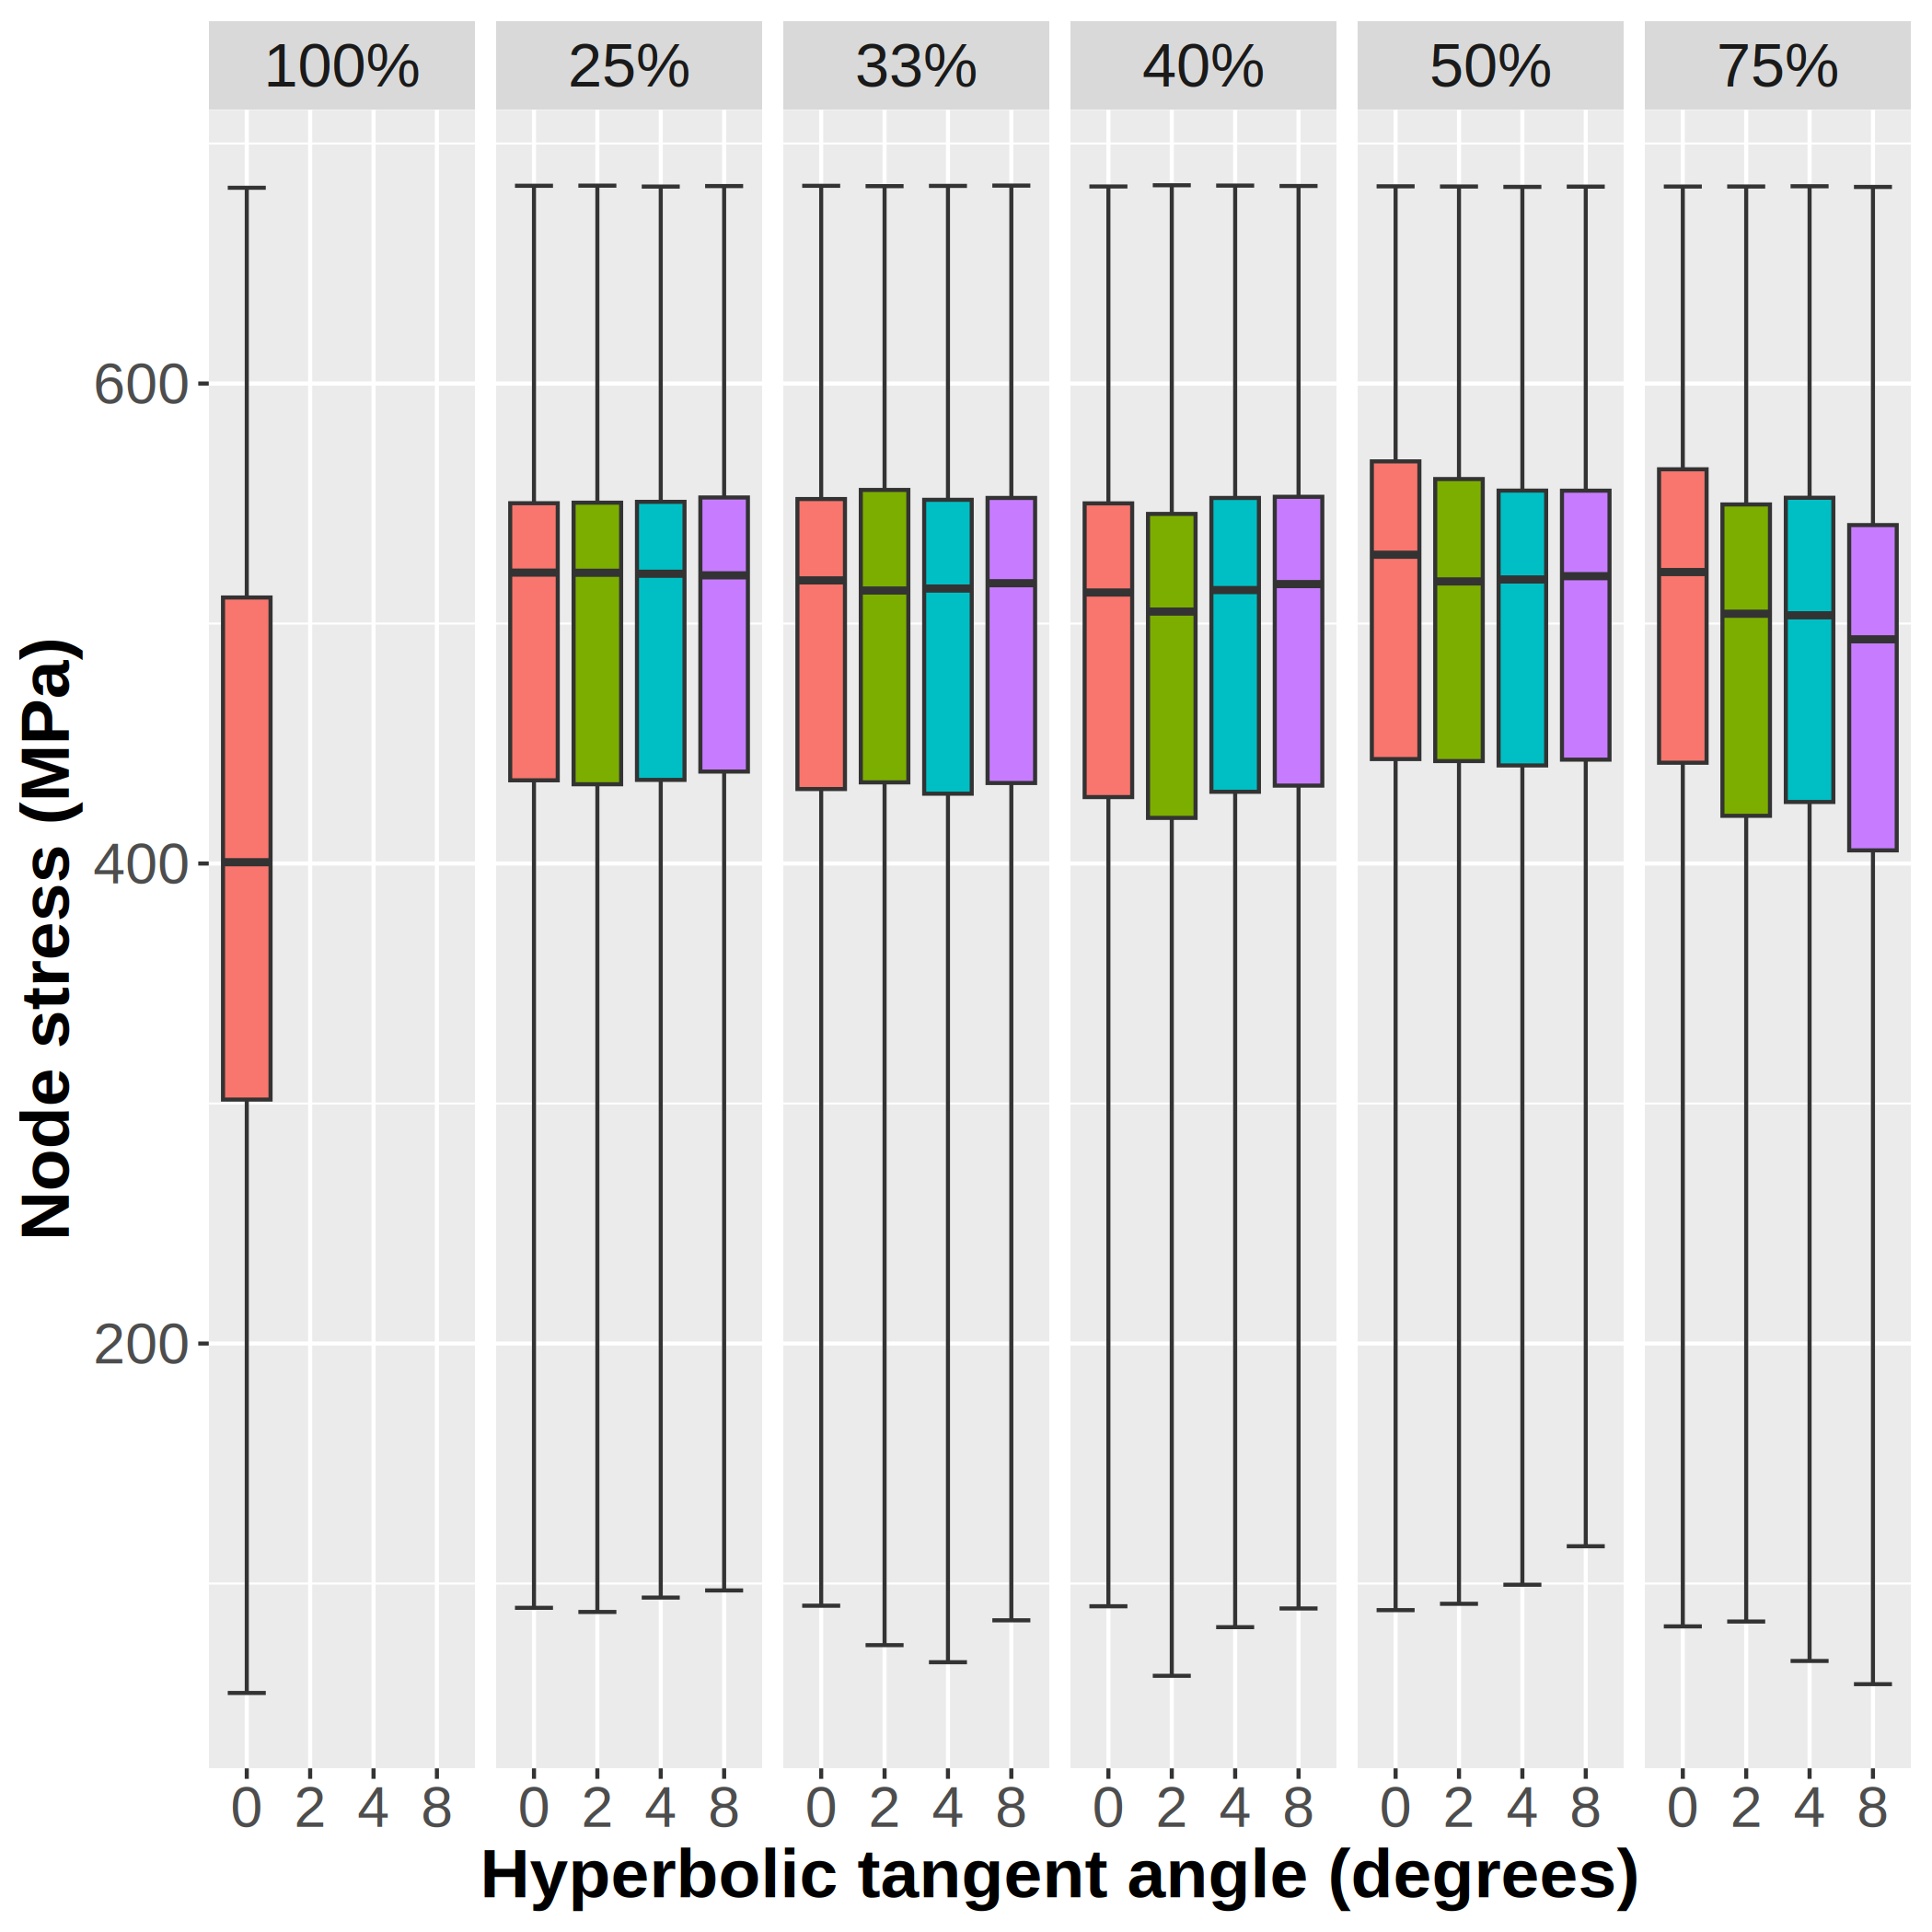
\includegraphics[width=0.8\textwidth]{images/results/plots/femoral/stress/boxplots.png}
  \caption{Box-and-whisker plot of nodal stress values of topologies of femoral component.}
  \label{fig:stress_boxwhisker}
\end{figure}

\end{document}
